\documentclass[12pt]{report}

%\usepackage{appendix}

\usepackage[margin=2cm]{geometry}
\geometry{letterpaper}
\setlength{\parindent}{0em}

\usepackage{array,booktabs}

\newcommand{\wood}{Bubinga}
\newcommand{\front}{aluminum}
\newcommand{\project}{Boogie Box}

%%%%%%%%%%%%%%%%%%%%%%%%%%%%%%%%%%%%%%%%%%%%%%%%%%%%%%%%%%%%%%%%%%%%%%%%%%%%%%%%
% Fonts
\usepackage{fontspec}

\newfontfamily\qag{TeX Gyre Adventor}
\newfontfamily\qbk{TeX Gyre Bonum}
\newfontfamily\ssfont[
  Path = fonts/,
  Extension = .ttf,
  UprightFont = *-Italic,
  ItalicFont = *-Italic,
  BoldFont = *-Italic,
  BoldItalicFont = *-Italic,
  Scale = 1.5,
]{DSEG7Classic}
\newfontfamily\ssfontinline[
  Path = fonts/,
  Extension = .ttf,
  UprightFont = *-Italic,
  ItalicFont = *-Italic,
  BoldFont = *-Italic,
  BoldItalicFont = *-Italic,
  Scale = 0.8,
]{DSEG7Classic}
\newfontfamily\ssfontsym[
  Path = fonts/,
  Extension = .ttf,
  UprightFont = *-Italic,
  ItalicFont = *-Italic,
  BoldFont = *-Italic,
  BoldItalicFont = *-Italic,
  Scale = 0.65,
]{DSEG7Classic}
%%%%%%%%%%%%%%%%%%%%%%%%%%%%%%%%%%%%%%%%%%%%%%%%%%%%%%%%%%%%%%%%%%%%%%%%%%%%%%%%

%%%%%%%%%%%%%%%%%%%%%%%%%%%%%%%%%%%%%%%%%%%%%%%%%%%%%%%%%%%%%%%%%%%%%%%%%%%%%%%%
% Tables
\usepackage{tabularx}
\usepackage{longtable}
\usepackage{tabu}
\usepackage{enumitem}
\usepackage{multirow}
%\usepackage{colortbl}
%\setlist{itemsep=1pt}
\setlist[enumerate]{label=(\textbf{\arabic*})}

%\multirow[vpos]{nrows}[bigstruts]{width}[vmove]{text}
%\newcolumntype{C}[1]{>{\centering\arraybackslash}m{#1}}
%\renewcommand{\tabularxcolumn}[1]{>{\small}m{#1}}

\tabcolsep=12pt
\renewcommand{\arraystretch}{1.3}

\newcommand{\ers}[1]{\extrarowsep=#1mm}

\newtabulinestyle{d=on 1pt off 1pt}
\newtabulinestyle{ld=on 4pt off 4pt}
\newcommand{\drule}[1]{\tabucline[d]{1-#1}}
\newcommand{\dcrule}[2]{\tabucline[d]{#1-#2}}
\newcommand{\lrule}[1]{\tabucline[ld]{1-#1}}
\newcommand{\lcrule}[2]{\tabucline[ld]{#1-#2}}
\newcommand{\thrule}{\toprule \hline}
\newcommand{\bhrule}{\hline \bottomrule}
\newcommand{\mdrule}{\hline \hline}
\newcommand{\mrule}{\hline}

\newcommand{\thm}[1]{\large #1}
\newcommand{\thb}[1]{\textbf{\large #1}}
\newcommand{\thi}[1]{\textit{\large #1}}
\newcommand{\thbi}[1]{\textbf{\textit{\large #1}}}
\newcommand{\thLb}[1]{\textbf{\Large #1}}

\newcommand{\as}[2]{%
\begin{table}[H]
\ers{0.1}
\centering
\begin{tabu} #1
\mrule
#2
\mrule
\end{tabu}
\end{table}}

\newcommand{\ase}[3]{%
\begin{table}[H]
\ers{#1}
\centering
\begin{tabu} #2
\mrule
#3
\mrule
\end{tabu}
\end{table}}

%%%%%%%%%%%%%%%%%%%%%%%%%%%%%%%%%%%%%%%%%%%%%%%%%%%%%%%%%%%%%%%%%%%%%%%%%%%%%%%%

%%%%%%%%%%%%%%%%%%%%%%%%%%%%%%%%%%%%%%%%%%%%%%%%%%%%%%%%%%%%%%%%%%%%%%%%%%%%%%%%
% Captions, Footnotes, References, TOC, etc.
\usepackage[bottom]{footmisc}
\usepackage{subcaption}
\usepackage[justification=centering]{caption}
%\captionsetup{font=scriptsize}
\captionsetup[sub]{font=scriptsize}
%\usepackage{footmisc}
\usepackage{titlesec}
\usepackage{tocloft}
%\setlength{\cftpartindent}{0em}
%\setlength{\cftpartnumwidth}{10em}

\setlength{\cftchapindent}{2.0em}
\setlength{\cftchapnumwidth}{2.0em}
\setlength{\cftsecindent}{4.0em}
\setlength{\cftsecnumwidth}{3.0em}
\setlength{\cftsubsecindent}{7.0em}
\setlength{\cftsubsecnumwidth}{3.5em}
\setlength{\cftsubsubsecindent}{10.5em}
\setlength{\cftsubsubsecnumwidth}{4.5em}
\renewcommand{\cftpartfont}{\bfseries\Large}
\renewcommand{\cftpartpagefont}{\bfseries\large}
\renewcommand{\cftchapfont}{\bfseries\large}
\renewcommand{\cftchappagefont}{\bfseries\normalsize}
\renewcommand{\cftsecfont}{\normalsize}
\renewcommand{\cftsubsecfont}{\normalsize}
\renewcommand{\cftsubsubsecfont}{\small}
\setlength{\cftbeforesecskip}{0.4em}
\setlength{\cftbeforesubsecskip}{0.2em}
\setlength{\cftbeforetabskip}{0.3em}
\setlength{\cftbeforefigskip}{0.3em}

\usepackage{hyperref}
\hypersetup {
colorlinks=true,
linkcolor=NavyBlue,
citecolor=blue,
filecolor=blue,
urlcolor=blue,
hyperfootnotes=true
}

\setcounter{tocdepth}{4}
%\setcounter{secnumdepth}{4}
\setcounter{secnumdepth}{3}
%%%%%%%%%%%%%%%%%%%%%%%%%%%%%%%%%%%%%%%%%%%%%%%%%%%%%%%%%%%%%%%%%%%%%%%%%%%%%%%%

%%%%%%%%%%%%%%%%%%%%%%%%%%%%%%%%%%%%%%%%%%%%%%%%%%%%%%%%%%%%%%%%%%%%%%%%%%%%%%%%
% Font sizes
%%%%%%%%%%%%%%%%%%%%%%%%%%%%%%%%%%%%%%%%%%%%%%%%%%%%%%%%%%%%%%%%%%%%%%%%%%%%%%%%
% \tiny
% \scriptsize
% \footnotesize
% \small
% \normalsize
% \large
% \Large
% \LARGE
% \huge
% \Huge
%%%%%%%%%%%%%%%%%%%%%%%%%%%%%%%%%%%%%%%%%%%%%%%%%%%%%%%%%%%%%%%%%%%%%%%%%%%%%%%%

%%%%%%%%%%%%%%%%%%%%%%%%%%%%%%%%%%%%%%%%%%%%%%%%%%%%%%%%%%%%%%%%%%%%%%%%%%%%%%%%
% titlesec
%%%%%%%%%%%%%%%%%%%%%%%%%%%%%%%%%%%%%%%%%%%%%%%%%%%%%%%%%%%%%%%%%%%%%%%%%%%%%%%%
%
% \titleformat{<command>}[<shape>]{<format>}{<label>}{<sep>}{<before-code>}[<after-code>]
%
% [<shape>] and [<after-code>] are optional parameters
%
% <command>
%   The sectioning command to be redefined:
%   \part, \chapter, \section, \subsection, \subsubsection, \paragraph or \subparagraph.
% <shape>
%   The sectioning paragraph shape. Possible values are:
%     hang, block, display, runin, leftmargin, rightmargin, drop, wrap, frame
% <format>
%   The format to be applied to the title, label, and text.
%   For example {\normalfont\Large\bfseries}
% <label>
%   Specify sectioning label.
% <sep>
%   The horizontal separation between label and title body and it must
%   be a length and not be empty.
% <before-code>
%   Code preceding the title body.
% <after-code>
%   Code following the title body.
%
%%%%%%%%%%%%%%%%%%%%%%%%%%%%%%%%%%%%%%%%%%%%%%%%%%%%%%%%%%%%%%%%%%%%%%%%%%%%%%%%
%
% \titlespacing{<command>}{<left>}{<before-sep>}{<after-sep>}
%
% <left>
%   Increases the left margin.
% <before-sep>
%   The vertical space before the title.
% <after-sep>
%   The separation between title and non-sectioning text.
%
%%%%%%%%%%%%%%%%%%%%%%%%%%%%%%%%%%%%%%%%%%%%%%%%%%%%%%%%%%%%%%%%%%%%%%%%%%%%%%%%
\usepackage{titletoc}

%\titlecontents{part}
%[3pc]
%{\addvspace{1.5pc}%
%\filcenter}
%{\thecontentslabel\\*[.2pc]%
%\bfseries\huge}
%{\bfseries\huge}
%{}  % That is, without page number
%[\addvspace{.5pc}]

%\titlecontents{part}
%[0pt]
%{\addvspace{1pc}%
%\itshape}%
%{\contentsmargin{0pt}%
%\bfseries
%\makebox[0pt][r]{\huge\thecontentslabel\enspace}%
%\large}
%{\contentsmargin{0pt}%
%\large}
%{\quad\thepage}
%[\addvspace{.5pc}]

\titleformat
{\part}
[frame]
{\bfseries\huge}
{\thepart}
{3.0ex}
{\centering}
[]

\titleformat
{\chapter} % command
%[display] % shape
[block] % shape
%{\bfseries\Large\itshape} % format
{\bfseries\LARGE} % format
%{Section \ \thechapter} % label
{\thechapter} % label
{1.0ex} % sep
{
    %\rule{\textwidth}{1pt}
    %\vspace{1ex}
    %\centering
} % before-code
[
\vspace{-0.5ex}%
\rule{\textwidth}{0.3pt}
] % after-code

\titleformat
{\section}
[block]
{\bfseries\Large}
{\thesection}
{0.5em}{}

\titleformat
{\subsection}
[block]
{\bfseries\large}
{\thesubsection}
{0.5em}{}

\titleformat
{\subsubsection}
[block]
{\bfseries}
{\thesubsubsection}
{0.5em}{}
%%%%%%%%%%%%%%%%%%%%%%%%%%%%%%%%%%%%%%%%%%%%%%%%%%%%%%%%%%%%%%%%%%%%%%%%%%%%%%%%

%%%%%%%%%%%%%%%%%%%%%%%%%%%%%%%%%%%%%%%%%%%%%%%%%%%%%%%%%%%%%%%%%%%%%%%%%%%%%%%%
% Graphics
\usepackage{graphicx}
\usepackage{float}
\usepackage[dvipsnames]{xcolor}
\usepackage[most]{tcolorbox}
%%%%%%%%%%%%%%%%%%%%%%%%%%%%%%%%%%%%%%%%%%%%%%%%%%%%%%%%%%%%%%%%%%%%%%%%%%%%%%%%

%%%%%%%%%%%%%%%%%%%%%%%%%%%%%%%%%%%%%%%%%%%%%%%%%%%%%%%%%%%%%%%%%%%%%%%%%%%%%%%%
% Symbols
\usepackage{bbding}  % For hand / Touch symbol

\usepackage{tikz}
\usetikzlibrary{bending,shapes.geometric}
%%%%%%%%%%%%%%%%%%%%%%%%%%%%%%%%%%%%%%%%%%%%%%%%%%%%%%%%%%%%%%%%%%%%%%%%%%%%%%%%

%%%%%%%%%%%%%%%%%%%%%%%%%%%%%%%%%%%%%%%%%%%%%%%%%%%%%%%%%%%%%%%%%%%%%%%%%%%%%%%%
% Commands
%%%%%%%%%%%%%%%%%%%%%%%%%%%%%%%%%%%%%%%%%%%%%%%%%%%%%%%%%%%%%%%%%%%%%%%%%%%%%%%%
% ------------------------------------------------------------------------------
%  General Options
% ------------------------------------------------------------------------------
%  opt:
%        n  Normal font
%        s  Small font
%        f  Footnotesize
%       ss  Scriptsize font
%        t  Tiny font
%      sym  Tikz overlay with Scriptsize font
%
%%%%%%%%%%%%%%%%%%%%%%%%%%%%%%%%%%%%%%%%%%%%%%%%%%%%%%%%%%%%%%%%%%%%%%%%%%%%%%%%

%%%%%%%%%%%%%%%%%%%%%%%%%%%%%%%%%%%%%%%%%%%%%%%%%%%%%%%%%%%%%%%%%%%%%%%%%%%%%%%%
% Base Commands
%%%%%%%%%%%%%%%%%%%%%%%%%%%%%%%%%%%%%%%%%%%%%%%%%%%%%%%%%%%%%%%%%%%%%%%%%%%%%%%%
\usepackage{ifthen}

\newcommand{\fontTGA}[2]{%
\ifthenelse{\equal{#1}{h}}{{\huge \qag #2}}{}%
\ifthenelse{\equal{#1}{l}}{{\large \qag #2}}{}%
\ifthenelse{\equal{#1}{n}}{{\qag #2}}{}%
\ifthenelse{\equal{#1}{s}}{{\small \qag #2}}{}%
\ifthenelse{\equal{#1}{f}}{{\footnotesize \qag #2}}{}%
%\ifthenelse{\equal{#1}{ss}}{{\textbf{\scriptsize \qag #2}}}{}%
\ifthenelse{\equal{#1}{ss}}{{\scriptsize \qag #2}}{}%
%\ifthenelse{\equal{#1}{t}}{{\textbf{\tiny \qag #2}}}{}}
\ifthenelse{\equal{#1}{t}}{{\tiny \qag #2}}{}}

% {fill color}{text color}{text}
\newcommand{\symTGA}[3]{% <--- XXX Remove space before comment marker to smoosh
\begin{tikz}[overlay]
  \node[fill=#1,draw=black,inner sep=1mm,anchor=text,rectangle,rounded corners=0.5mm]
    %at (0.06,0.03) {\color{#2} \fontTGA{ss}{#3}};
    at (0.06,0.03) {\color{#2} \fontTGA{ss}{#3}};
\end{tikz}% <--- XXX Remove space before comment marker to smoosh
\phantom{\fontTGA{ss}{#3}}}% <--- XXX Remove space before comment marker to smoosh

\newcommand{\symTGAL}[3]{% <--- XXX Remove space before comment marker to smoosh
\vspace{-5ex}\begin{flushright}
\begin{tikz}[overlay]
  \node[fill=#1,draw=black,inner sep=1.5mm,anchor=text,rectangle,rounded corners=1.0mm,thick]
    %at (0.06,0.03) {\color{#2} \fontTGA{ss}{#3}};
    at (0.06,0.03) {\color{#2} \textbf{\fontTGA{n}{#3}}};
\end{tikz}% <--- XXX Remove space before comment marker to smoosh
\phantom{\fontTGA{n}{#3}}\end{flushright}\vskip 1.5ex}% <--- XXX Remove space before comment marker to smoosh
%%%%%%%%%%%%%%%%%%%%%%%%%%%%%%%%%%%%%%%%%%%%%%%%%%%%%%%%%%%%%%%%%%%%%%%%%%%%%%%%

%%%%%%%%%%%%%%%%%%%%%%%%%%%%%%%%%%%%%%%%%%%%%%%%%%%%%%%%%%%%%%%%%%%%%%%%%%%%%%%%
% Operation
%%%%%%%%%%%%%%%%%%%%%%%%%%%%%%%%%%%%%%%%%%%%%%%%%%%%%%%%%%%%%%%%%%%%%%%%%%%%%%%%
% Controls & Screens
\newcommand{\control}[2]{%
\ifthenelse{\equal{#1}{sym}}{\symTGA{black}{white}{#2}}{\fontTGA{#1}{#2}}}

% Positions, Directions & Times
\newcommand{\direction}[2]{%
\ifthenelse{\equal{#1}{sym}}{\symTGA{black!50}{white}{#2}}{\fontTGA{#1}{#2}}}

% Actions
\newcommand{\action}[2]{%
\ifthenelse{\equal{#1}{sym}}{\symTGA{black!10}{black}{#2}}{\fontTGA{#1}{#2}}}
% )))2 %%%%%%%%%%%%%%%%%%%%%%%%%%%%%%%%%%%%%%%%%%%%%%%%%%%%%%%%%%%%%%%%%%%%%%%%%

%%%%%%%%%%%%%%%%%%%%%%%%%%%%%%%%%%%%%%%%%%%%%%%%%%%%%%%%%%%%%%%%%%%%%%%%%%%%%%%%
% Operational Elements
%%%%%%%%%%%%%%%%%%%%%%%%%%%%%%%%%%%%%%%%%%%%%%%%%%%%%%%%%%%%%%%%%%%%%%%%%%%%%%%%
% Components & Modes
\newcommand{\mode}[2]{%
\ifthenelse{\equal{#1}{sym}}{\symTGA{black}{white}{#2}}{%
\ifthenelse{\equal{#1}{syml}}{\symTGAL{black}{white}{#2}}{\fontTGA{#1}{#2}}}}

\newcommand{\symMode}[1]{%
\begin{tikzpicture}[scale=0.1, minimum height=1.2cm]
  \draw[fill=black,text=white] (0,0) circle [radius=5] node {\mode{t}{#1}};
\end{tikzpicture}}

% Menus
\newcommand{\menu}[2]{%
\ifthenelse{\equal{#1}{sym}}{\symTGA{black!50}{white}{#2}}{%
\ifthenelse{\equal{#1}{syml}}{\symTGAL{black!50}{white}{#2}}{\fontTGA{#1}{#2}}}}

\newcommand{\symMenu}[1]{%
\begin{tikzpicture}[scale=0.1, minimum height=1.2cm]
  \draw[fill=black!50,text=white] (0,0) circle [radius=5] node {\menu{t}{#1}};
\end{tikzpicture}}

% States
\newcommand{\state}[2]{%
\ifthenelse{\equal{#1}{sym}}{\symTGA{black!10}{black}{#2}}{%
\ifthenelse{\equal{#1}{syml}}{\symTGAL{black!10}{black}{#2}}{\fontTGA{#1}{#2}}}}

\newcommand{\symState}[1]{%
\begin{tikzpicture}[scale=0.1, minimum height=1.2cm]
  \draw[fill=black!10,text=black] (0,0) circle [radius=5] node {\state{t}{#1}};
\end{tikzpicture}}

\newcommand{\symUnidirectional}{%
\begin{tikzpicture}[scale=0.2]
  \draw[->,>=stealth,ultra thick] (0,0) -- (10,0);
\end{tikzpicture}}

\newcommand{\symUniModule}{%
\begin{tikzpicture}[scale=0.1]
  \draw[->,>=stealth,thick] (0,0) -- (10,0);
  \draw[fill=black,text=white] (-5,0) circle [radius=5] node {\state{t}{MODULE}};
  \draw[fill=black!10,text=black] (15,0) circle [radius=5] node {\state{t}{STATE}};
\end{tikzpicture}}

\newcommand{\symUniMenu}{%
\begin{tikzpicture}[scale=0.1]
  \draw[->,>=stealth,thick] (0,0) -- (10,0);
  \draw[fill=black!50,text=white] (-5,0) circle [radius=5] node {\state{t}{MENU}};
  \draw[fill=black!10,text=black] (15,0) circle [radius=5] node {\state{t}{STATE}};
\end{tikzpicture}}

\newcommand{\symUniState}{%
\begin{tikzpicture}[scale=0.1]
  \draw[->,>=stealth,thick] (0,0) -- (10,0);
  \draw[fill=black!10,text=black] (-5,0) circle [radius=5] node {\state{t}{STATE}};
  \draw[fill=black!10,text=black] (15,0) circle [radius=5] node {\state{t}{STATE}};
\end{tikzpicture}}

\newcommand{\symUniStateAction}{%
\begin{tikzpicture}[scale=0.1]
  \draw[->,>=stealth,thick] (0,0) -- node[above] {\action{t}{ACTION}} (30,0);
  \draw[fill=black!10,text=black] (-3,0) circle [radius=3] node {\state{t}{A}};
  \draw[fill=black!10,text=black] (33,0) circle [radius=3] node {\state{t}{B}};
\end{tikzpicture}}

\newcommand{\symUniSameState}{%
\begin{tikzpicture}[scale=0.1]
  \draw[->,thick] (0,-2.5) arc (-60:-310:3);
  \path node at (-9,0) {\action{t}{ACTION}};
  \draw[fill=black!10,text=black] (4,0) circle [radius=4] node {\state{ss}{A}};
\end{tikzpicture}}

\newcommand{\symBidirectional}{%
\begin{tikzpicture}[scale=0.2]
  \draw[<->,>=stealth,ultra thick] (0,0) -- (10,0);
\end{tikzpicture}}

\newcommand{\symBiState}{%
\begin{tikzpicture}[scale=0.1]
  \draw[<->,>=stealth,thick] (0,0) -- (50,0);
  \path node at (10,2) {\action{t}{ACTION} \raisebox{0.3mm}{\tiny{\scalebox{0.8}{to}}} \state{t}{A}};
  \path node at (40,2) {\action{t}{ACTION} \raisebox{0.3mm}{\tiny{\scalebox{0.8}{to}}} \state{t}{B}};
  \draw[fill=black!10,text=black] (-3,0) circle [radius=3] node {\state{t}{A}};
  \draw[fill=black!10,text=black] (53,0) circle [radius=3] node {\state{t}{B}};
\end{tikzpicture}}

\newcommand{\symBiStateOne}{%
  \begin{tikzpicture}[scale=0.1]
  \draw[<->,>=stealth,thick] (0,0) -- node[above] {\action{t}{ACTION}} (30,0);
  \draw[fill=black!10,text=black] (-3,0) circle [radius=3] node {\state{t}{A}};
  \draw[fill=black!10,text=black] (33,0) circle [radius=3] node {\state{t}{B}};
\end{tikzpicture}}

\newcommand{\symNode}{%
  \begin{tikzpicture}[scale=0.2]
  \draw[fill=black] (0,0) circle [radius=0.6];
  \draw[<-,>=stealth,ultra thick] (0,5) -- (0,-5);
  \draw[ultra thick] (-5,0) -- (5,0);
\end{tikzpicture}}

\newcommand{\symNodeState}{%
  \begin{tikzpicture}[scale=0.1]
  \draw[fill=black] (0,0) circle [radius=0.6];
  \draw[<-,>=stealth,thick] (0,10) -- (0,0);
  \draw[thick] (-30,0) -- node[above]
    {\action{t}{ACTION} \raisebox{0.3mm}{\tiny{\scalebox{0.8}{to}}} \state{t}{C}} (0,0);
  \draw[thick] (0,0) -- node[above]
    {\action{t}{ACTION} \raisebox{0.3mm}{\tiny{\scalebox{0.8}{to}}} \state{t}{C}} (30,0);
  \draw[fill=black!10,text=black] (0,13) circle [radius=3] node {\state{t}{C}};
  \draw[fill=black!10,text=black] (-33,0) circle [radius=3] node {\state{t}{A}};
  \draw[fill=black!10,text=black] (33,0) circle [radius=3] node {\state{t}{B}};
\end{tikzpicture}}

%%%%%%%%%%%%%%%%%%%%%%%%%%%%%%%%%%%%%%%%%%%%%%%%%%%%%%%%%%%%%%%%%%%%%%%%%%%%%%%%

%%%%%%%%%%%%%%%%%%%%%%%%%%%%%%%%%%%%%%%%%%%%%%%%%%%%%%%%%%%%%%%%%%%%%%%%%%%%%%%%
% Effects
%%%%%%%%%%%%%%%%%%%%%%%%%%%%%%%%%%%%%%%%%%%%%%%%%%%%%%%%%%%%%%%%%%%%%%%%%%%%%%%%
\newcommand{\eDi}[2]{%
\ifthenelse{\equal{#1}{sym}}{\symTGA{white}{black}{DISPLAY #2}}{\fontTGA{#1}{DISPLAY #2}}}

\newcommand{\eLi}[2]{%
\ifthenelse{\equal{#1}{sym}}{\symTGA{white}{black}{LIGHT #2}}{\fontTGA{#1}{LIGHT #2}}}

\newcommand{\ePl}[2]{%
\ifthenelse{\equal{#1}{sym}}{\symTGA{green}{black}{PLAY #2}}{\fontTGA{#1}{PLAY #2}}}

\newcommand{\eRewind}[2]{%
\ifthenelse{\equal{#1}{sym}}{\symTGA{blue}{white}{REWIND #2}}{\fontTGA{#1}{REWIND #2}}}

\newcommand{\eResume}[2]{%
\ifthenelse{\equal{#1}{sym}}{\symTGA{green}{black}{RESUME #2}}{\fontTGA{#1}{RESUME #2}}}

\newcommand{\ePa}[2]{%
\ifthenelse{\equal{#1}{sym}}{\symTGA{yellow}{black}{PAUSE #2}}{\fontTGA{#1}{PAUSE #2}}}

\newcommand{\eSt}[2]{%
\ifthenelse{\equal{#1}{sym}}{\symTGA{red}{white}{STOP #2}}{\fontTGA{#1}{STOP #2}}}

\newcommand{\eSk}[2]{%
\ifthenelse{\equal{#1}{sym}}{\symTGA{blue}{white}{SKIP #2}}{\fontTGA{#1}{SKIP #2}}}

\newcommand{\eAc}[2]{%
\ifthenelse{\equal{#1}{sym}}{\symTGA{blue}{white}{#2}}{\fontTGA{#1}{#2}}}

\newcommand{\eNAc}[2]{%
\ifthenelse{\equal{#1}{sym}}{\symTGA{red}{white}{#2}}{\fontTGA{#1}{#2}}}

\newcommand{\eStart}[2]{%
\ifthenelse{\equal{#1}{sym}}{\symTGA{green}{black}{START #2}}{\fontTGA{#1}{START #2}}}

\newcommand{\eEn}[2]{%
\ifthenelse{\equal{#1}{sym}}{\symTGA{green}{black}{ENABLE #2}}{\fontTGA{#1}{ENABLE #2}}}

\newcommand{\eSnooze}[2]{%
\ifthenelse{\equal{#1}{sym}}{\symTGA{yellow}{black}{SNOOZE #2}}{\fontTGA{#1}{SNOOZE #2}}}

\newcommand{\eWake}[2]{%
\ifthenelse{\equal{#1}{sym}}{\symTGA{green}{black}{WAKE #2}}{\fontTGA{#1}{WAKE #2}}}

\newcommand{\eTo}[2]{%
\ifthenelse{\equal{#1}{sym}}{\symTGA{orange}{black}{TOGGLE #2}}{\fontTGA{#1}{TOGGLE #2}}}

\newcommand{\eRe}[2]{%
\ifthenelse{\equal{#1}{sym}}{\symTGA{red}{white}{RESET #2}}{\fontTGA{#1}{RESET #2}}}

\newcommand{\eAl}[1]{%
\ifthenelse{\equal{#1}{sym}}{\symTGA{red!70}{white}{ALERT}}{\fontTGA{#1}{ALERT}}}

\newcommand{\eSe}[2]{%
\ifthenelse{\equal{#1}{sym}}{\symTGA{green}{black}{SET #2}}{\fontTGA{#1}{SET #2}}}

\newcommand{\eSel}[2]{%
\ifthenelse{\equal{#1}{sym}}{\symTGA{green!50!blue}{white}{SELECT #2}}{\fontTGA{#1}{SET #2}}}

\newcommand{\eBl}[2]{%
\ifthenelse{\equal{#1}{sym}}{\symTGA{white}{black}{BLINK #2}}{\fontTGA{#1}{BLINK #2}}}

\newcommand{\eUp}[2]{%
\ifthenelse{\equal{#1}{sym}}{\symTGA{yellow}{black}{UPDATE #2}}{\fontTGA{#1}{UPDATE #2}}}

\newcommand{\eSa}[2]{%
\ifthenelse{\equal{#1}{sym}}{\symTGA{blue}{white}{SAVE #2}}{\fontTGA{#1}{SAVE #2}}}

\newcommand{\eCa}[2]{%
\ifthenelse{\equal{#1}{sym}}{\symTGA{blue!30}{black}{CACHE #2}}{\fontTGA{#1}{CACHE #2}}}

\newcommand{\eReset}[1]{%
\ifthenelse{\equal{#1}{sym}}{\symTGA{red}{white}{RESET}}{\fontTGA{#1}{RESET}}}

\newcommand{\eCM}[1]{%
\ifthenelse{\equal{#1}{sym}}{\symTGA{purple!80!black!70}{white}{CHANGE MODE}}{\fontTGA{#1}{CHANGE MODE}}}

\newcommand{\eRu}[2]{%
\ifthenelse{\equal{#1}{sym}}{\symTGA{blue!70}{white}{#2 RUN}}{\fontTGA{#1}{#2 RUN}}}

\newcommand{\eCo}[2]{%
\ifthenelse{\equal{#1}{sym}}{\symTGA{blue!70}{white}{#2 COMPLETE}}{\fontTGA{#1}{#2 COMPLETE}}}

\newcommand{\eLo}[2]{%
\ifthenelse{\equal{#1}{sym}}{\symTGA{blue!70}{white}{LOAD #2}}{\fontTGA{#1}{LOAD #2}}}

\newcommand{\eDisable}[2]{%
\ifthenelse{\equal{#1}{sym}}{\symTGA{red}{white}{DISABLE #2}}{\fontTGA{#1}{DISABLE #2}}}

%%%%%%%%%%%%%%%%%%%%%%%%%%%%%%%%%%%%%%%%%%%%%%%%%%%%%%%%%%%%%%%%%%%%%%%%%%%%%%%%
% Error Severity Levels
%%%%%%%%%%%%%%%%%%%%%%%%%%%%%%%%%%%%%%%%%%%%%%%%%%%%%%%%%%%%%%%%%%%%%%%%%%%%%%%%
\newcommand{\symSevTGA}[3]{% <--- XXX Remove space before comment marker to smoosh
\begin{tikz}[overlay]
  \node[fill=#1,draw=black,inner sep=1mm,anchor=text,rectangle,rounded corners=0.5mm]
    %at (0.06,0.03) {\color{#2} \fontTGA{ss}{#3}};
    at (0.06,0.03) {\color{#2} \fontTGA{s}{#3}};
\end{tikz}% <--- XXX Remove space before comment marker to smoosh
\phantom{\fontTGA{s}{#3}}}% <--- XXX Remove space before comment marker to smoosh

\newcommand{\sNormal}[1]{%
\ifthenelse{\equal{#1}{sym}}{\symSevTGA{blue}{white}{NORMAL}}{\fontTGA{#1}{NORMAL}}}

\newcommand{\sLow}[1]{%
\ifthenelse{\equal{#1}{sym}}{\symSevTGA{green}{black}{LOW}}{\fontTGA{#1}{LOW}}}

\newcommand{\sMedium}[1]{%
\ifthenelse{\equal{#1}{sym}}{\symSevTGA{yellow}{black}{MEDIUM}}{\fontTGA{#1}{MEDIUM}}}

\newcommand{\sHigh}[1]{%
\ifthenelse{\equal{#1}{sym}}{\symSevTGA{red}{white}{HIGH}}{\fontTGA{#1}{HIGH}}}
%%%%%%%%%%%%%%%%%%%%%%%%%%%%%%%%%%%%%%%%%%%%%%%%%%%%%%%%%%%%%%%%%%%%%%%%%%%%%%%%

%%%%%%%%%%%%%%%%%%%%%%%%%%%%%%%%%%%%%%%%%%%%%%%%%%%%%%%%%%%%%%%%%%%%%%%%%%%%%%%%
% Controls & Screens
%%%%%%%%%%%%%%%%%%%%%%%%%%%%%%%%%%%%%%%%%%%%%%%%%%%%%%%%%%%%%%%%%%%%%%%%%%%%%%%%
\newcommand{\cRs}[1]{\control{#1}{SELECTOR DIAL}}
\newcommand{\cEs}[1]{\control{#1}{SETTINGS KNOB}}
\newcommand{\cBr}[1]{\control{#1}{BRIGHTNESS KNOB}}
\newcommand{\cLB}[1]{\control{#1}{LOW BATTERY INDICATOR}}
\newcommand{\cPo}[1]{\control{#1}{POWER SWITCH}}
\newcommand{\cVo}[1]{\control{#1}{VOLUME}}
\newcommand{\cPl}[1]{\control{#1}{PLAY|PAUSE|STOP}}
\newcommand{\cNe}[1]{\control{#1}{NEXT}}
\newcommand{\cPr}[1]{\control{#1}{PREVIOUS}}
\newcommand{\cTS}[1]{\control{#1}{TOUCH SENSOR}}
\newcommand{\cDi}[1]{\control{#1}{DISPLAY}}
\newcommand{\cLi}[1]{\control{#1}{LIGHTING}}
\newcommand{\cBe}[1]{\control{#1}{BEEPER}}
\newcommand{\cPA}[1]{\control{#1}{POWER ADAPTER}}
\newcommand{\cPP}[1]{\control{#1}{POWER / CHARGE PORT}}
\newcommand{\cUSB}[1]{\control{#1}{USB 2.0 MICRO-B}}
\newcommand{\cRB}[1]{\control{#1}{RECHARGEABLE BATTERY}}
\newcommand{\cCC}[1]{\control{#1}{COIN CELL BATTERY}}
\newcommand{\cMSD}[1]{\control{#1}{MICRO SD CARD}}
\newcommand{\cEE}[1]{\control{#1}{EEPROM}}
\newcommand{\cTo}[1]{\control{#1}{TOP}}
\newcommand{\cFr}[1]{\control{#1}{FRONT}}
\newcommand{\cSi}[1]{\control{#1}{SIDES}}
\newcommand{\cLS}[1]{\control{#1}{LEFT SIDE}}
\newcommand{\cRS}[1]{\control{#1}{RIGHT SIDE}}
\newcommand{\cBa}[1]{\control{#1}{BACK}}
\newcommand{\cBo}[1]{\control{#1}{BOTTOM}}
\newcommand{\cMi}[1]{\control{#1}{MICROCONTROLLER}}
\newcommand{\cSp}[1]{\control{#1}{SPEAKERS}}
\newcommand{\cPS}[1]{\control{#1}{POWER SUPPLY}}
\newcommand{\cEn}[1]{\control{#1}{ENCLOSURE}}
\newcommand{\cCB}[1]{\control{#1}{CIRCUIT BOARD}}
\newcommand{\cAD}[1]{\control{#1}{AUDIO DECODER}}
\newcommand{\cAm}[1]{\control{#1}{AMPLIFIER}}

\newcommand{\sBe}{%
\begin{tikzpicture}[scale=0.1]
  \draw[fill=black] (0,0) circle [radius=1];
  \draw[fill=white] (0,0) circle [radius=0.25];

  \draw (1.3,0.75) arc (30:-30:1.5);
  \draw (1.73,1) arc (30:-30:2);
  \draw (2.17,1.25) arc (30:-30:2.5);

%  \draw[rotate=90] (1.3,0.75) arc (30:-30:1.5);
%  \draw[rotate=90] (1.73,1) arc (30:-30:2);
%  \draw[rotate=90] (2.17,1.25) arc (30:-30:2.5);
%
%  \draw[rotate=-90] (1.3,0.75) arc (30:-30:1.5);
%  \draw[rotate=-90] (1.73,1) arc (30:-30:2);
%  \draw[rotate=-90] (2.17,1.25) arc (30:-30:2.5);

  \draw[rotate=180] (1.3,0.75) arc (30:-30:1.5);
  \draw[rotate=180] (1.73,1) arc (30:-30:2);
  \draw[rotate=180] (2.17,1.25) arc (30:-30:2.5);
\end{tikzpicture}}

\newcommand{\sNBe}{%
\begin{tikzpicture}[scale=0.1,baseline=-3.5]
  \draw[fill=black] (0,0) circle [radius=1];

  \draw (1.3,0.75) arc (30:-30:1.5);
  \draw (1.73,1) arc (30:-30:2);
  \draw (2.17,1.25) arc (30:-30:2.5);
  \draw[rotate=180] (1.3,0.75) arc (30:-30:1.5);
  \draw[rotate=180] (1.73,1) arc (30:-30:2);
  \draw[rotate=180] (2.17,1.25) arc (30:-30:2.5);

  \draw[thick] (2,2) -- (-2,-2);
  \draw[thick] (-2,2) -- (2,-2);
  \draw[fill=white] (0,0) circle [radius=0.25];
\end{tikzpicture}}

%%%%%%%%%%%%%%%%%%%%%%%%%%%%%%%%%%%%%%%%%%%%%%%%%%%%%%%%%%%%%%%%%%%%%%%%%%%%%%%%

%%%%%%%%%%%%%%%%%%%%%%%%%%%%%%%%%%%%%%%%%%%%%%%%%%%%%%%%%%%%%%%%%%%%%%%%%%%%%%%%
% Positions, Directions & Times
%%%%%%%%%%%%%%%%%%%%%%%%%%%%%%%%%%%%%%%%%%%%%%%%%%%%%%%%%%%%%%%%%%%%%%%%%%%%%%%%
\newcommand{\dLe}[1]{\direction{#1}{LEFT}}
\newcommand{\dRi}[1]{\direction{#1}{RIGHT}}
\newcommand{\dMi}[1]{\direction{#1}{MIDDLE}}
\newcommand{\dTo}[1]{\direction{#1}{TOP}}
\newcommand{\dFo}[1]{\direction{#1}{FORWARD}}
\newcommand{\dBa}[1]{\direction{#1}{BACKWARD}}
\newcommand{\dRe}[1]{\direction{#1}{REWIND}}
\newcommand{\dCl}[1]{\direction{#1}{CLOCKWISE}}
\newcommand{\dCC}[1]{\direction{#1}{COUNTER-CLOCKWISE}}
\newcommand{\secs}[2]{%
\ifthenelse{\equal{#1}{sym}}{\direction{#1}{#2 SECS}}{\direction{#1}{#2 SECONDS}}}
\newcommand{\mins}[2]{%
\ifthenelse{\equal{#1}{sym}}{\direction{#1}{#2 MINS}}{\direction{#1}{#2 MINUTES}}}
\newcommand{\hours}[2]{%
\ifthenelse{\equal{#1}{sym}}{\direction{#1}{#2 HRS}}{\direction{#1}{#2 HOURS}}}

\newcommand{\mono}[1]{\texttt{\textbf{#1}}}
\newcommand{\num}[1]{\mono{#1}}
%%%%%%%%%%%%%%%%%%%%%%%%%%%%%%%%%%%%%%%%%%%%%%%%%%%%%%%%%%%%%%%%%%%%%%%%%%%%%%%%

%%%%%%%%%%%%%%%%%%%%%%%%%%%%%%%%%%%%%%%%%%%%%%%%%%%%%%%%%%%%%%%%%%%%%%%%%%%%%%%%
% Actions
%%%%%%%%%%%%%%%%%%%%%%%%%%%%%%%%%%%%%%%%%%%%%%%%%%%%%%%%%%%%%%%%%%%%%%%%%%%%%%%%
\newcommand{\aTu}[1]{\action{#1}{TURN}}
\newcommand{\sTu}{%
\begin{tikzpicture}[scale=0.1,thick,baseline=-8.5]
  \draw[<->] (0,0) arc (70:-250:1.75);
\end{tikzpicture}}

\newcommand{\aTuN}[1]{\action{#1}{TURN N TIMES}}
\newcommand{\sTuN}[1]{%
\begin{tikzpicture}[scale=0.1,thick,baseline=-8.5]
  \draw[<->] (0,0) arc (70:-250:1.75) node[anchor=west] at (0.5,-1.8) {\fontTGA{ss}{#1}};
\end{tikzpicture}}

\newcommand{\aCl}[1]{\action{#1}{TURN CLOCKWISE}}
\newcommand{\sCl}{%
\begin{tikzpicture}[scale=0.1,thick,baseline=-8.5]
  \draw[->] (0,0) arc (70:-250:1.75);
\end{tikzpicture}}

\newcommand{\aCC}[1]{\action{#1}{TURN COUNTER-CLOCKWISE}}
\newcommand{\sCC}{%
\begin{tikzpicture}[scale=0.1,thick,baseline=-8.5]
  \draw[<-] (0,0) arc (70:-250:1.75);
\end{tikzpicture}}

\newcommand{\sNTu}{%
\begin{tikzpicture}[scale=0.1,thick,baseline=-9]
  \draw[<->] (0,0) arc (70:-250:1.75);
  \draw (-2.65,0.25) -- (1.55,-3.75);
  \draw (1.55,0.25) -- (-2.65,-3.75);
\end{tikzpicture}}

\newcommand{\sNTuN}[1]{%
\begin{tikzpicture}[scale=0.1,thick,baseline=-9]
  \draw[<->] (0,0) arc (70:-250:1.75) node[anchor=west] at (0.7,-1.8) {\fontTGA{ss}{#1s}};
  \draw (-2.65,0.25) -- (1.55,-3.75);
  \draw (1.55,0.25) -- (-2.65,-3.75);
\end{tikzpicture}}

\newcommand{\aPr}[1]{\action{#1}{PRESS}}

\newcommand{\aRe}[1]{\action{#1}{RELEASE}}
\newcommand{\sRe}{%
\begin{tikzpicture}[scale=0.1,thick]
  \draw[->] (0,0) -- (0,4);
\end{tikzpicture}}

\newcommand{\aPR}[1]{\action{#1}{PRESS \& RELEASE}}
\newcommand{\sPR}{%
\begin{tikzpicture}[scale=0.1,thick,baseline=2]
  \draw[->] (0,4) -- (0,0);
  \draw[->] (1.5,0) -- (1.5,4);
\end{tikzpicture}}

\newcommand{\sPRN}[1]{%
\begin{tikzpicture}[scale=0.1,thick,baseline=2]
  \draw[->] (0,4) -- (0,0);
  %\draw[->] (1.5,0) -- (1.5,4);
  %\node[anchor=west] (2.5,4) {\fontTGA{ss}{#1}};
  \draw[->] (1.5,0) -- (1.5,4) node[anchor=west] at (1.1,1.8) {\fontTGA{ss}{#1}};
\end{tikzpicture}}

\newcommand{\sNPR}{%
\begin{tikzpicture}[scale=0.1,thick,baseline=2]
  \draw[->] (0,4) -- (0,0);
  \draw[->] (1.5,0) -- (1.5,4);
  \draw (-1.5,4) -- (3,0);
  \draw (3,4) -- (-1.5,0);
\end{tikzpicture}}

\newcommand{\sNPRN}[1]{%
\begin{tikzpicture}[scale=0.1,thick,baseline=2]
  \draw[->] (0,4) -- (0,0);
  \draw[->] (1.5,0) -- (1.5,4) node[anchor=west] at (2.0,2) {\fontTGA{ss}{#1s}};
  \draw (-1.5,4) -- (3,0);
  \draw (3,4) -- (-1.5,0);
\end{tikzpicture}}

\newcommand{\aPH}[1]{\action{#1}{PRESS \& HOLD}}
\newcommand{\sPH}{%
\begin{tikzpicture}[scale=0.1,thick,baseline=2]
  \draw (0,0) -- (3,0);
  \draw[->] (1.5,4) -- (1.5,0.5);
\end{tikzpicture}}

\newcommand{\sPHN}[1]{%
\begin{tikzpicture}[scale=0.1,thick,baseline=2]
  \draw (0,0) -- (3,0);
  \draw[->] (1.5,4) -- (1.5,0.5) node[anchor=west] at (2.0,2) {\fontTGA{ss}{#1s}};
\end{tikzpicture}}

\newcommand{\aSC}[1]{\action{#1}{SINGLE-CLICK}}
\newcommand{\sSC}{\sPR}

\newcommand{\aDC}[1]{\action{#1}{DOUBLE-CLICK}}
\newcommand{\sDC}{%
\begin{tikzpicture}[scale=0.1,thick,baseline=2]
  \draw[->>] (0,4) -- (0,0);
  \draw[->>] (1.5,0) -- (1.5,4);
\end{tikzpicture}}

\newcommand{\aSe}[1]{\action{#1}{SELECT}}

\newcommand{\aTo}[1]{\action{#1}{TOUCH}}
%\newcommand{\sTo}{\HandCuffLeft}
\newcommand{\sTo}{\raisebox{-0.8mm}{\HandCuffLeft}}
%\newcommand{\sToN}[1]{\HandCuffLeft\thinspace \raisebox{1.2mm}{\fontTGA{ss}{#1s}}}
\newcommand{\sToN}[1]{%
\raisebox{-0.8mm}{\HandCuffLeft}\thinspace \raisebox{0.4mm}{\fontTGA{ss}{#1s}}}

% No Touch
\newcommand{\sNTo}{%
\begin{tikzpicture}[scale=0.2,thick,baseline=-3.5]
  %\node (0,0) {\HandCuffLeft};
  %\draw[fill=black,rotate=45] (-0.08,-1.4) rectangle (0.08,1.4);
  %\draw[fill=black,rotate=-45] (-0.08,-1.4) rectangle (0.08,1.4);
  \node (0,0) {\raisebox{-0.8mm}{\HandCuffLeft}};
  \draw (-1,-1) -- (1,1);
  \draw (-1,1) -- (1,-1);
\end{tikzpicture}}

\newcommand{\sNToN}[1]{%
%\begin{tikzpicture}[scale=0.2,ultra thin,baseline=-3.5]
\begin{tikzpicture}[scale=0.2,thick,baseline=-3.5]
  %\node (0,0) {\raisebox{-0.8mm}{\HandCuffLeft}\thinspace \raisebox{0.4mm}{\fontTGA{ss}{#1s}}};
  %\draw[fill=black,rotate=45] (-0.08,-1.4) rectangle (0.02,1.4);
  %\draw[fill=black,rotate=-45] (-0.08,-1.4) rectangle (0.02,1.4);
  %\draw[fill=black,rotate=45] (-0.10,-1.4) rectangle (0.0,1.4);
  %\draw[fill=black,rotate=-45] (-0.10,-1.4) rectangle (0.0,1.4);
  %\draw (-2.25,-1) -- (-0.25,1);
  %\draw (-2.25,1) -- (-0.25,-1);
  \node at (-0.5,0) {\raisebox{-0.8mm}{$\hskip -3mm$ \HandCuffLeft}};
  \node at (1.5,0) {\raisebox{0.4mm}{\fontTGA{ss}{#1s}}};
  \draw (-2,-1) -- (0,1);
  \draw (-2,1) -- (0,-1);
\end{tikzpicture}}

\newcommand{\aReset}[1]{\action{#1}{RESET}}

\newcommand{\sBarOne}{%
\begin{tikzpicture}[scale=0.1,thick,baseline=2]
  \draw (0,0) -- (3,0);
  \draw[->] (1.5,4) -- (1.5,0.5);
  \draw[->] (4,0) -- (4,4);
\end{tikzpicture}}

% Press & Hold for 2 Bars
\newcommand{\sBarTwo}{%
\begin{tikzpicture}[scale=0.1,thick,baseline=2]
  \draw (0,0) -- (3,0);
  \draw (0,0.5) -- (3,0.5);
  \draw[->] (1.5,4) -- (1.5,1);
  \draw[->] (4,0) -- (4,4);
\end{tikzpicture}}

% Press & Hold for 3 Bars
\newcommand{\sBarThree}{%
\begin{tikzpicture}[scale=0.1,thick,baseline=2]
  \draw (0,0) -- (3,0);
  \draw (0,0.5) -- (3,0.5);
  \draw (0,1) -- (3,1);
  \draw[->] (1.5,4) -- (1.5,1.5);
  \draw[->] (4,0) -- (4,4);
\end{tikzpicture}}

\newcommand{\sReset}{\sBarOne}
\newcommand{\sSec}{\sBarTwo}
\newcommand{\sTer}{\sBarThree}

% Audio
\newcommand{\sPl}{%
\begin{tikzpicture}[scale=0.1,rounded corners=1,baseline=-3]
  \draw[fill=black] (-5.2,-2) -- (-5.2,2) -- (-2.3,0) -- cycle;

  \draw[fill=black] (-1.3,-1.7) rectangle (-0.3,1.7);
  \draw[fill=black] (0.3,-1.7) rectangle (1.3,1.7);

  \draw[fill=black] (2.5,-1.7) rectangle (5.5,1.7);
\end{tikzpicture}}

\newcommand{\sNe}{%
\begin{tikzpicture}[scale=0.1,rounded corners=1,baseline=-3]
  \draw[fill=black] (-1.5,-2) -- (-1.5,2) -- (1.4,0) -- cycle;
  \draw[fill=black,rounded corners=0.5] (1.5,-2) rectangle (1.9,2);
\end{tikzpicture}}

\newcommand{\sPr}{%
\begin{tikzpicture}[scale=0.1,rounded corners=1,baseline=-3]
  \draw[fill=black] (1.5,-2) -- (1.5,2) -- (-1.4,0) -- cycle;
  \draw[fill=black,rounded corners=0.5] (-1.5,-2) rectangle (-1.9,2);
\end{tikzpicture}}

\newcommand{\aPlay}[1]{\action{#1}{PLAY}}
\newcommand{\sPlay}{%
\begin{tikzpicture}[scale=0.1,rounded corners=1,baseline=-4]
  %\draw[fill=black] (0,0) -- (0,4) -- (3,2) -- cycle;
  \draw[fill=black!10] (0,0) circle [radius=3.5];
  \draw[fill=black] (-1.2,-2) -- (-1.2,2) -- (1.7,0) -- cycle;
\end{tikzpicture}}

\newcommand{\aPause}[1]{\action{#1}{PAUSE}}
\newcommand{\sPause}{%
\begin{tikzpicture}[scale=0.1,rounded corners=1,baseline=-4]
  %\draw (0,0) rectangle (1,4);
  %\draw (1.75,0) rectangle (2.75,4);
  \draw[fill=black!10] (0,0) circle [radius=3.5];
  \draw[fill=black] (-1.3,-1.7) rectangle (-0.3,1.7);
  \draw[fill=black] (0.3,-1.7) rectangle (1.3,1.7);
\end{tikzpicture}}

\newcommand{\aStop}[1]{\action{#1}{STOP}}
\newcommand{\sStop}{%
\begin{tikzpicture}[scale=0.1,rounded corners=1,baseline=-4]
  %\draw (0,0) rectangle (4,4);
  \draw[fill=black!10] (0,0) circle [radius=3.5];
  \draw[fill=black] (-1.5,-1.5) rectangle (1.5,1.5);
\end{tikzpicture}}

\newcommand{\aSkip}[1]{\action{#1}{SKIP}}

\newcommand{\aNext}[1]{\action{#1}{NEXT}}
\newcommand{\sNext}{%
\begin{tikzpicture}[scale=0.1,rounded corners=1,baseline=-4]
  %\draw (0,0) -- (0,4) -- (3,2) -- cycle;
  %\draw (3.25,0) rectangle (4.0,4);
  \draw[fill=black!10] (0,0) circle [radius=3.5];
  \draw[fill=black] (-1.6,-2) -- (-1.6,2) -- (1.3,0) -- cycle;
  \draw[fill=black,rounded corners=0.5] (1.4,-2) rectangle (1.8,2);
\end{tikzpicture}}

\newcommand{\aPrev}[1]{\action{#1}{PREVIOUS}}
\newcommand{\sPrev}{%
\begin{tikzpicture}[scale=0.1,rounded corners=1,baseline=-4]
  %\draw (0,0) rectangle (0.75,4);
  %\draw (1.0,2) -- (4.0,4) -- (4.0,0) -- cycle;
  \draw[fill=black!10] (0,0) circle [radius=3.5];
  \draw[fill=black] (1.6,-2) -- (1.6,2) -- (-1.3,0) -- cycle;
  \draw[fill=black,rounded corners=0.5] (-1.4,-2) rectangle (-1.8,2);
\end{tikzpicture}}

% Display & Lighting (Screen) states
\newcommand{\sScOn}[1]{\state{#1}{ON}}
\newcommand{\sScOf}[1]{\state{#1}{OFF}}
\newcommand{\sScDi}[1]{\state{#1}{DIM}}

\newcommand{\eOn}[2]{%
\ifthenelse{\equal{#1}{sym}}{\symTGA{white}{black}{#2 ON}}{\fontTGA{#1}{#2 ON}}}

\newcommand{\eDim}[2]{%
\ifthenelse{\equal{#1}{sym}}{\symTGA{white}{black!50}{#2 DIM}}{\fontTGA{#1}{#2 DIM}}}

\newcommand{\eOff}[2]{%
\ifthenelse{\equal{#1}{sym}}{\symTGA{black}{white}{#2 OFF}}{\fontTGA{#1}{#2 OFF}}}

\newcommand{\sOn}[1]{%
\ifthenelse{\equal{#1}{sym}}{\symTGA{white}{black}{ON}}{\fontTGA{#1}{ON}}}

\newcommand{\sDim}[1]{%
\ifthenelse{\equal{#1}{sym}}{\symTGA{black!50}{white}{DIM}}{\fontTGA{#1}{DIM}}}

\newcommand{\sOff}[1]{%
\ifthenelse{\equal{#1}{sym}}{\symTGA{black}{white}{OFF}}{\fontTGA{#1}{OFF}}}
%%%%%%%%%%%%%%%%%%%%%%%%%%%%%%%%%%%%%%%%%%%%%%%%%%%%%%%%%%%%%%%%%%%%%%%%%%%%%%%%

%%%%%%%%%%%%%%%%%%%%%%%%%%%%%%%%%%%%%%%%%%%%%%%%%%%%%%%%%%%%%%%%%%%%%%%%%%%%%%%%
% Components
%%%%%%%%%%%%%%%%%%%%%%%%%%%%%%%%%%%%%%%%%%%%%%%%%%%%%%%%%%%%%%%%%%%%%%%%%%%%%%%%
% Audio
\newcommand{\mAu}[1]{\mode{#1}{AUDIO}}
\newcommand{\sAuPl}[1]{\state{#1}{PLAY}}
\newcommand{\sAuPa}[1]{\state{#1}{PAUSE}}
\newcommand{\sAuSt}[1]{\state{#1}{STOP}}
\newcommand{\sAuNe}[1]{\state{#1}{NEXT}}
\newcommand{\sAuPr}[1]{\state{#1}{PREVIOUS}}
\newcommand{\sAuSk}[1]{\state{#1}{SKIP}}
\newcommand{\sAuOc}[1]{\state{#1}{OCCUPIED}}

% Alarm
\newcommand{\mAl}[1]{\mode{#1}{ALARM}}
\newcommand{\sAlDi}[1]{\state{#1}{DISABLED}}
\newcommand{\sAlWa}[1]{\state{#1}{WAKE}}
\newcommand{\sAlSn}[1]{\state{#1}{SNOOZE}}
\newcommand{\sAlOf}[1]{\state{#1}{OFF}}
\newcommand{\sAlSt}[1]{\state{#1}{STOPPED}}
\newcommand{\sAlIP}[1]{\state{#1}{IN PROGRESS}}

\newcommand{\aTi}[1]{%
\ifthenelse{\equal{#1}{sym}}{\symTGA{blue}{white}{TIME $=$ ALARM TIME}}{\fontTGA{#1}{TIME $=$ ALARM TIME}}}
\newcommand{\aWT}[1]{%
\ifthenelse{\equal{#1}{sym}}{\symTGA{blue}{white}{WAKE TIME EXCEEDED}}{\fontTGA{#1}{WAKE TIME EXCEEDED}}}
\newcommand{\aTT}[1]{%
\ifthenelse{\equal{#1}{sym}}{\symTGA{blue}{white}{TOTAL ALARM TIME EXCEEDED}}{\fontTGA{#1}{TOTAL ALARM TIME EXCEEDED}}}
\newcommand{\aST}[1]{%
\ifthenelse{\equal{#1}{sym}}{\symTGA{blue}{white}{SNOOZE TIME EXPIRED}}{\fontTGA{#1}{SNOOZE TIME EXPIRED}}}

% Power
\newcommand{\mPo}[1]{\mode{#1}{POWER}}
\newcommand{\sPoAw}[1]{\state{#1}{WAKE}}
\newcommand{\sPoSl}[1]{\state{#1}{SLEEP}}
\newcommand{\sPoNa}[1]{\state{#1}{NAP}}
%%%%%%%%%%%%%%%%%%%%%%%%%%%%%%%%%%%%%%%%%%%%%%%%%%%%%%%%%%%%%%%%%%%%%%%%%%%%%%%%

%%%%%%%%%%%%%%%%%%%%%%%%%%%%%%%%%%%%%%%%%%%%%%%%%%%%%%%%%%%%%%%%%%%%%%%%%%%%%%%%
% Modes, Menus and States
%%%%%%%%%%%%%%%%%%%%%%%%%%%%%%%%%%%%%%%%%%%%%%%%%%%%%%%%%%%%%%%%%%%%%%%%%%%%%%%%
\newcommand{\mPr}[1]{\mode{#1}{PRIMARY}}
\newcommand{\mSe}[1]{\mode{#1}{SECONDARY}}
\newcommand{\mTe}[1]{\mode{#1}{TERTIARY}}

\newcommand{\sON}[1]{\state{#1}{ON}}
\newcommand{\sOFF}[1]{\state{#1}{OFF}}

% Clock
\newcommand{\mCl}[1]{\mode{#1}{CLOCK}}
% States
\newcommand{\sClTi}[1]{\state{#1}{TIME}}
\newcommand{\sClMD}[1]{\state{#1}{MONTH \& DAY}}
\newcommand{\sClYe}[1]{\state{#1}{YEAR}}
\newcommand{\sClSh}[1]{\state{#1}{SHOW TRACK}}
\newcommand{\sClSe}[1]{\state{#1}{SET TRACK}}

% Timer
\newcommand{\mTi}[1]{\mode{#1}{TIMER}}
% States
\newcommand{\sTiHM}[1]{\state{#1}{SET H|M}}
\newcommand{\sTiMS}[1]{\state{#1}{SET M|S}}
\newcommand{\sTiRu}[1]{\state{#1}{RUN}}
\newcommand{\sTiPa}[1]{\state{#1}{PAUSE}}
\newcommand{\sTiAl}[1]{\state{#1}{ALERT}}
\newcommand{\sTiWa}[1]{\state{#1}{WAIT}}

% Set Alarm
\newcommand{\mSA}[1]{\mode{#1}{SET ALARM}}
% States
\newcommand{\sSAHo}[1]{\state{#1}{HOUR}}
\newcommand{\sSAMi}[1]{\state{#1}{MINUTE}}
\newcommand{\sSAWS}[1]{\state{#1}{WAKEUP SOURCE}}
\newcommand{\sSAST}[1]{\state{#1}{SNOOZE TIME}}
\newcommand{\sSAWT}[1]{\state{#1}{WAKE TIME}}
\newcommand{\sSATT}[1]{\state{#1}{TOTAL ALARM TIME}}
\newcommand{\sSADo}[1]{\state{#1}{DONE}}
\newcommand{\sSADi}[1]{\state{#1}{DISABLED}}

% Set Clock
\newcommand{\mSC}[1]{\mode{#1}{SET CLOCK}}
% States
\newcommand{\sSCFo}[1]{\state{#1}{FORMAT}}
\newcommand{\sSCHo}[1]{\state{#1}{HOUR}}
\newcommand{\sSCMi}[1]{\state{#1}{MINUTE}}
\newcommand{\sSCYe}[1]{\state{#1}{YEAR}}
\newcommand{\sSCMo}[1]{\state{#1}{MONTH}}
\newcommand{\sSCDa}[1]{\state{#1}{DAY}}
\newcommand{\sSCDS}[1]{\state{#1}{DST}}
\newcommand{\sSCDo}[1]{\state{#1}{DONE}}

% Power Settings
\newcommand{\mPS}[1]{\mode{#1}{POWER SETTINGS}}
% Menu
\newcommand{\mPSNa}[1]{\menu{#1}{NAP}}
\newcommand{\mPSSt}[1]{\menu{#1}{STOP}}
\newcommand{\mPSSl}[1]{\menu{#1}{SLEEP}}
\newcommand{\mPSTo}[1]{\menu{#1}{TOUCH}}
% States
\newcommand{\sPSMe}[1]{\state{#1}{MENU}}
\newcommand{\sPSHM}[1]{\state{#1}{H|M}}
\newcommand{\sPSMS}[1]{\state{#1}{M|S}}
\newcommand{\sPSSe}[1]{\state{#1}{SECONDS}}
\newcommand{\sPSDo}[1]{\state{#1}{DONE}}

% Touch Settings
\newcommand{\mTS}[1]{\mode{#1}{TOUCH SETTINGS}}
% Menu
\newcommand{\mTSCa}[1]{\menu{#1}{CALIBRATE}}
\newcommand{\mTSRe}[1]{\menu{#1}{READ}}
\newcommand{\mTSCo}[1]{\menu{#1}{CONFIGURE}}
\newcommand{\mTSDe}[1]{\menu{#1}{DEFAULTS}}
\newcommand{\mTSDi}[1]{\menu{#1}{DISABLE}}
% States
\newcommand{\sTSMe}[1]{\state{#1}{MENU}}
\newcommand{\sTSDi}[1]{\state{#1}{DISABLED}}
\newcommand{\sTSNS}[1]{\state{#1}{NSCN}}
\newcommand{\sTSPS}[1]{\state{#1}{PS}}
\newcommand{\sTSRC}[1]{\state{#1}{REFCHRG}}
\newcommand{\sTSEC}[1]{\state{#1}{EXTCHRG}}
\newcommand{\sTSWB}[1]{\state{#1}{WAIT BASELINE}}
\newcommand{\sTSBR}[1]{\state{#1}{BASELINE RUN}}
\newcommand{\sTSWT}[1]{\state{#1}{WAIT TOUCH}}
\newcommand{\sTSTR}[1]{\state{#1}{TOUCH RUN}}
\newcommand{\sTSRT}[1]{\state{#1}{TOUCH \& READ}}
\newcommand{\sTSTA}[1]{\state{#1}{TEST \& ADJUST}}
\newcommand{\sTSDo}[1]{\state{#1}{DONE}}

% Set Night Light
\newcommand{\mSN}[1]{\mode{#1}{SET NIGHT LIGHT}}
% Night Light Menu
\newcommand{\mSNOn}[1]{\menu{#1}{COLOR \#1}}
\newcommand{\mSNTw}[1]{\menu{#1}{COLOR \#2}}
\newcommand{\mSNTh}[1]{\menu{#1}{COLOR \#3}}
% Color Menu
\newcommand{\mSNCo}[1]{\menu{#1}{PRESET}}
\newcommand{\mSNRGB}[1]{\menu{#1}{RGB}}
\newcommand{\mSNHSB}[1]{\menu{#1}{HSB}}
% States
\newcommand{\sSNMN}[1]{\state{#1}{COLOR MENU}}
\newcommand{\sSNMC}[1]{\state{#1}{METHOD MENU}}
\newcommand{\sSNCI}[1]{\state{#1}{COLOR}}
\newcommand{\sSNRe}[1]{\state{#1}{RED}}
\newcommand{\sSNGr}[1]{\state{#1}{GREEN}}
\newcommand{\sSNBl}[1]{\state{#1}{BLUE}}
\newcommand{\sSNHu}[1]{\state{#1}{HUE}}
\newcommand{\sSNSa}[1]{\state{#1}{SATURATION}}
\newcommand{\sSNBr}[1]{\state{#1}{BRIGHTNESS}}
\newcommand{\sSNDo}[1]{\state{#1}{DONE}}
%%%%%%%%%%%%%%%%%%%%%%%%%%%%%%%%%%%%%%%%%%%%%%%%%%%%%%%%%%%%%%%%%%%%%%%%%%%%%%%%

%%%%%%%%%%%%%%%%%%%%%%%%%%%%%%%%%%%%%%%%%%%%%%%%%%%%%%%%%%%%%%%%%%%%%%%%%%%%%%%%
% Rotary Switch
%%%%%%%%%%%%%%%%%%%%%%%%%%%%%%%%%%%%%%%%%%%%%%%%%%%%%%%%%%%%%%%%%%%%%%%%%%%%%%%%
\newcommand{\sRs}[1]{%
\begin{tikzpicture}[scale=0.1,thick]
  \draw[fill=black] (0,0) circle [radius=2];
  \draw[fill=black,rotate=#1] (2,1.5) arc (30:150:2.25) -- (0,6) -- cycle;
  \node at (7,7) {};
  \node at (-7,-7) {};
\end{tikzpicture}}

\newcommand{\sLe}{\sRs{90}}
\newcommand{\sMi}{\sRs{180}}
\newcommand{\sRi}{\sRs{-90}}

\newcommand{\sLM}{%
\begin{tikzpicture}[scale=0.1,thick]
  \draw[fill=black] (0,4) circle [radius=2];
  \draw[fill=black] (-1.5,6) arc (120:240:2.25) -- (-6,4) -- cycle;
  \draw[fill=black] (0,-4) circle [radius=2];
  \draw[fill=black] (-2,-5.5) arc (210:330:2.25) -- (0,-10) -- cycle;
  \node at (-8,8) {};
  \node at (8,-12) {};
\end{tikzpicture}}

\newcommand{\sLtoM}{%
\begin{tikzpicture}[scale=0.1,thick,baseline=4]
  \draw[fill=black] (0,4) circle [radius=2];
  \draw[fill=black!20,color=black!20] (-1.5,6) arc (120:240:2.25) -- (-6,4) -- cycle;
  \draw[fill=black] (-2,2.5) arc (210:330:2.25) -- (0,-2) -- cycle;
  \draw[->] (-5.5,3.5) arc (180:270:5.0);
  %\node at (-2,9) {};
  %\node at (5,-4) {};
\end{tikzpicture}}

\newcommand{\sMtoL}{%
\begin{tikzpicture}[scale=0.1,thick,baseline=4]
  \draw[fill=black] (0,4) circle [radius=2];
  \draw[fill=black] (-1.5,6) arc (120:240:2.25) -- (-6,4) -- cycle;
  \draw[fill=black!20,color=black!20] (-2,2.5) arc (210:330:2.25) -- (0,-2) -- cycle;
  \draw[<-] (-5.5,3.5) arc (180:270:5.0);
  %\node at (-2,9) {};
  %\node at (5,-4) {};
\end{tikzpicture}}

\newcommand{\sMtoR}{%
\begin{tikzpicture}[scale=0.1,thick,baseline=-6]
  \draw[fill=black,rotate=90] (0,4) circle [radius=2];
  \draw[fill=black!20,color=black!20,thick,rotate=90] (-1.5,6) arc (120:240:2.25) -- (-6,4) -- cycle;
  \draw[fill=black,thick,rotate=90] (-2,2.5) arc (210:330:2.25) -- (0,-2) -- cycle;
  \draw[->,rotate=90] (-5.5,3.5) arc (180:270:5.0);
  %\node at (-10,5) {};
  %\node at (2,-8) {};
  %\node at (-7,2) {};
  %\node at (2,2) {};
\end{tikzpicture}}

\newcommand{\sRtoM}{%
\begin{tikzpicture}[scale=0.1,thick,baseline=-6]
  \draw[fill=black,rotate=90] (0,4) circle [radius=2];
  \draw[fill=black,rotate=90] (-1.5,6) arc (120:240:2.25) -- (-6,4) -- cycle;
  \draw[fill=black!20,color=black!20,rotate=90] (-2,2.5) arc (210:330:2.25) -- (0,-2) -- cycle;
  \draw[<-,rotate=90] (-5.5,3.5) arc (180:270:5.0);
  %\node at (-10,5) {};
  %\node at (2,-8) {};
  %\node at (-8,1) {};
  %\node at (4,-4) {};
\end{tikzpicture}}

\newcommand{\sRM}{%
\begin{tikzpicture}[scale=0.1,thick]
  \draw[fill=black] (0,4) circle [radius=2];
  \draw[fill=black] (1.5,6) arc (60:-60:2.25) -- (6,4) -- cycle;
  \draw[fill=black] (0,-4) circle [radius=2];
  \draw[fill=black] (-2,-5.5) arc (210:330:2.25) -- (0,-10) -- cycle;
  \node at (-8,8) {};
  \node at (8,-12) {};
\end{tikzpicture}}

\newcommand{\sLR}{%
\begin{tikzpicture}[scale=0.1,thick]
  \draw[fill=black] (0,4) circle [radius=2];
  \draw[fill=black] (-1.5,6) arc (120:240:2.25) -- (-6,4) -- cycle;
  \draw[fill=black] (0,-4) circle [radius=2];
  \draw[fill=black] (1.5,-2) arc (60:-60:2.25) -- (6,-4) -- cycle;
  \node at (-8,8) {};
  \node at (8,-12) {};
\end{tikzpicture}}

\newcommand{\sLtoR}{%
\begin{tikzpicture}[scale=0.1,thick,baseline=6]
  \draw[fill=black] (0,4) circle [radius=2];
  \draw[fill=black!20,color=black!20] (-1.5,6) arc (120:240:2.25) -- (-6,4) -- cycle;
  \draw[fill=black] (1.5,6) arc (60:-60:2.25) -- (6,4) -- cycle;
  \draw[->] (-5.5,3.5) arc (180:360:5.5);
  %\node at (-6.5,10) {};
  %\node at (8,-5) {};
\end{tikzpicture}}

\newcommand{\sRtoL}{%
\begin{tikzpicture}[scale=0.1,thick,baseline=6]
  \draw[fill=black] (0,4) circle [radius=2];
  \draw[fill=black] (-1.5,6) arc (120:240:2.25) -- (-6,4) -- cycle;
  \draw[fill=black!20,color=black!20] (1.5,6) arc (60:-60:2.25) -- (6,4) -- cycle;
  \draw[<-] (-5.5,3.5) arc (180:360:5.5);
  %\node at (-6.5,10) {};
  %\node at (8,-5) {};
\end{tikzpicture}}
%%%%%%%%%%%%%%%%%%%%%%%%%%%%%%%%%%%%%%%%%%%%%%%%%%%%%%%%%%%%%%%%%%%%%%%%%%%%%%%%

%%%%%%%%%%%%%%%%%%%%%%%%%%%%%%%%%%%%%%%%%%%%%%%%%%%%%%%%%%%%%%%%%%%%%%%%%%%%%%%%
% Seven Segment Display
%%%%%%%%%%%%%%%%%%%%%%%%%%%%%%%%%%%%%%%%%%%%%%%%%%%%%%%%%%%%%%%%%%%%%%%%%%%%%%%%
% {phantom text}{text}
\newcommand{\sSSD}[2]{%
\begin{tikzpicture}[baseline]
\node[anchor=base,fill=black!80,draw=black,inner sep=2.5pt,rounded corners=0.5mm]
  {\color{white} \phantom{\ssfontinline #1}};
\node[anchor=base,inner sep=2.5pt,rounded corners=0.5mm]
  {\color{white} \ssfontinline #2};
\end{tikzpicture}}

\newcommand{\symSSD}[2]{%
\begin{tikzpicture}[baseline]
  \node[anchor=base,fill=black!80,draw=black,inner sep=0.7mm,rounded corners=0.5mm]
    {\color{white} \phantom{\ssfontsym #1}};
  \node[anchor=base,inner sep=0.7mm,rounded corners=0.5mm]
    {\color{white} \ssfontsym #2};
\end{tikzpicture}}

% {phantom text}{text}
\newcommand{\sSSDl}[2]{%
\begin{tikzpicture}[baseline]
  \node[anchor=base,fill=black!80,draw=black,inner sep=4pt,rounded corners=0.5mm]
    {\color{white} \phantom{\ssfont #1}};
  \node[anchor=base,inner sep=4pt,rounded corners=0.5mm]
    {\color{white} \ssfont #2};
\end{tikzpicture}}

% For inline text
\newcommand{\sD}[1]{{\sSSD{8.8.:8.8.}{#1}}}
\newcommand{\sDs}[1]{{\sSSD{8}{#1}}}
\newcommand{\symD}[1]{{\symSSD{8.8.:8.8.}{#1}}}

% For figures
\newcommand{\sDl}[1]{{\sSSDl{8.8.:8.8.}{#1}}}
\newcommand{\sDls}[1]{{\sSSDl{8}{#1}}}
\newcommand{\figD}[2]{%
\begin{table}[H]
\ers{0.1}
\centering
\begin{tabu}{c}
\sDl{#1} \\
\scriptsize #2 \\
\end{tabu}
\end{table}}

\newcommand{\figDT}[4]{%
\begin{table}[H]
\ers{0.1}
\centering
\begin{tabu} to 4in {X[1,c,m] X[1,c,m]}
\sDl{#1} & \sDl{#3} \\
\scriptsize #2 & \scriptsize #4 \\
\end{tabu}
\end{table}}

%%%%%%%%%%%%%%%%%%%%%%%%%%%%%%%%%%%%%%%%%%%%%%%%%%%%%%%%%%%%%%%%%%%%%%%%%%%%%%%%

%%%%%%%%%%%%%%%%%%%%%%%%%%%%%%%%%%%%%%%%%%%%%%%%%%%%%%%%%%%%%%%%%%%%%%%%%%%%%%%%
% Color Symbols
%%%%%%%%%%%%%%%%%%%%%%%%%%%%%%%%%%%%%%%%%%%%%%%%%%%%%%%%%%%%%%%%%%%%%%%%%%%%%%%%
\newcommand{\symColor}[3]{% <--- XXX Remove space before comment marker to smoosh
%\begin{tikzpicture}[overlay]
\begin{tikzpicture}[baseline=2]
  %\node[fill=#1,draw=black,inner sep=3pt,anchor=text,rectangle,rounded corners=0.5mm]
    %at (0.06,0.03) {\color{#2} \fontTGA{n}{#3}};
  \draw[fill=#1,draw=black,inner sep=1mm,rectangle,rounded corners=0.5mm]
    (0,0) rectangle node {\color{#2} \fontTGA{ss}{#3}} (1.7,0.4);
\end{tikzpicture} % <--- XXX Remove space before comment marker to smoosh
%\phantom{\fontTGA{n}{GGGGGG}}} % <--- XXX Remove space before comment marker to smoosh
} % <--- XXX Remove space before comment marker to smoosh

\newcommand{\cBl}{\symColor{blue}{white}{BLUE}}
\newcommand{\cGr}{\symColor{green}{black}{GREEN}}
\newcommand{\cYe}{\symColor{yellow}{black}{YELLOW}}
\newcommand{\cOr}{\symColor{orange}{black}{ORANGE}}
\newcommand{\cRe}{\symColor{red}{white}{RED}}
\newcommand{\cPu}{\symColor{violet}{white}{PURPLE}}
\newcommand{\cPi}{\symColor{pink}{white}{PINK}}

\newcommand{\cCol}[3]{\symColor{#1}{#2}{#3}}

%%%%%%%%%%%%%%%%%%%%%%%%%%%%%%%%%%%%%%%%%%%%%%%%%%%%%%%%%%%%%%%%%%%%%%%%%%%%%%%%
\newcommand{\ddfrac}[2]{\frac{\displaystyle #1}{\displaystyle #2}}

\setlength{\fboxsep}{12pt}

\newcommand{\danger}[1]{\begin{center}\fbox{%
\begin{minipage}{0.94\textwidth}%
{\raisebox{-1.1mm}{
\includegraphics{images/danger.png}} #1}%
\end{minipage}}\end{center}}

\newcommand{\warning}[1]{\begin{center}\fbox{%
\begin{minipage}{0.94\textwidth}%
{\raisebox{-1.1mm}{
\includegraphics{images/warning.png}} #1}%
\end{minipage}}\end{center}}

\newcommand{\info}[1]{\begin{center}\fbox{%
\begin{minipage}{0.94\textwidth}%
{\raisebox{-1.2mm}{
\includegraphics{images/info.png}} #1}%
\end{minipage}}\end{center}}

\newcommand{\cbox}[1]{\begin{center}\fcolorbox{black!20}{black!2}{%
\begin{minipage}{0.95\textwidth}#1\end{minipage}}\end{center}}

\newcommand{\steps}[2]{\begin{center}\begin{tcolorbox}[breakable, enhanced]%
\par\medskip%
{\parbox{\textwidth}{\centering \thbi{#1}}} \newline #2%
\end{tcolorbox}\end{center}}

%%%%%%%%%%%%%%%%%%%%%%%%%%%%%%%%%%%%%%%%%%%%%%%%%%%%%%%%%%%%%%%%%%%%%%%%%%%%%%%%

%%%%%%%%%%%%%%%%%%%%%%%%%%%%%%%%%%%%%%%%%%%%%%%%%%%%%%%%%%%%%%%%%%%%%%%%%%%%%%%%
% Title Info
%\title{}
%\author{}
%\date{\today}
%%%%%%%%%%%%%%%%%%%%%%%%%%%%%%%%%%%%%%%%%%%%%%%%%%%%%%%%%%%%%%%%%%%%%%%%%%%%%%%%

%%%%%%%%%%%%%%%%%%%%%%%%%%%%%%%%%%%%%%%%%%%%%%%%%%%%%%%%%%%%%%%%%%%%%%%%%%%%%%%%
% Begin Document %%%%%%%%%%%%%%%%%%%%%%%%%%%%%%%%%%%%%%%%%%%%%%%%%%%%%%%%%%%%%%%
%%%%%%%%%%%%%%%%%%%%%%%%%%%%%%%%%%%%%%%%%%%%%%%%%%%%%%%%%%%%%%%%%%%%%%%%%%%%%%%%
\begin{document}

\thispagestyle{empty}

\begin{table}[H]
\begin{tabu}{X[1,l,m] X[1,r,m]}
  \fontTGA{h}{\bfseries \project{}}
    & \fontTGA{ss}{Designed, Coded and Assembled by Todd Wease} \\
\end{tabu}
\end{table}

\begin{table}[H]
\ers{3}
\begin{tabu}{X[1,l,m] X[1,l,m]}
  \multirow{4}{*}{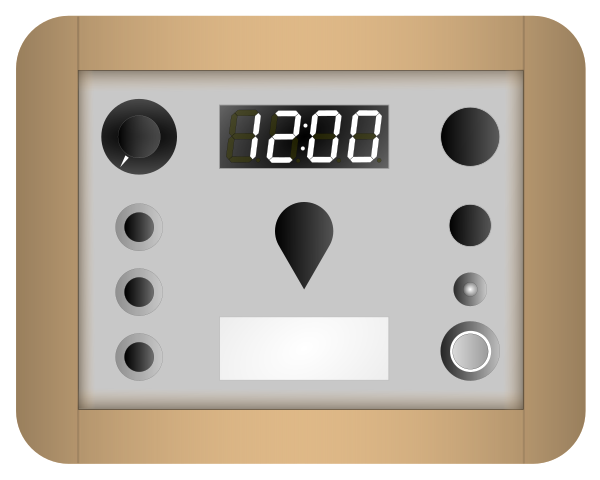
\includegraphics{images/alarm_clock.png}}
    & \fontTGA{n}{Portable with Rechargeable Lithium Ion Battery} \\
  & \fontTGA{n}{Micro USB connection for Powering and Charging} \\
  & \fontTGA{n}{Low Battery Indicator} \\
  & \fontTGA{n}{Controllable Display and Lighting Brightness} \\
\end{tabu}
\end{table}

\begin{table}[H]
\begin{tabu}{X[1,l,p] X[1,l,p]}
  \fontTGA{s}{\bfseries Clock}
  \footnotesize \qag
  \begin{itemize}[label=, leftmargin=1pt, itemsep=1pt]
    \item Date \& Time
    \item 12 or 24 Hour Time Format
    \item Configurable Daylight Saving Time
    \item Coin Cell Battery backup keeps time when device is unpowered
  \end{itemize}
  &
  \fontTGA{s}{\bfseries Alarm}
  \footnotesize \qag
  \begin{itemize}[label=, leftmargin=1pt, itemsep=1pt]
    \item Wake to Beeper or Audio
    \item Touch to Snooze
    \item Configurable Snooze Time
    \item Configurable Auto-Stop Timers
  \end{itemize}
\end{tabu}
\end{table}

\begin{table}[H]
\begin{tabu}{X[1,l,p] X[1,l,p]}
  \fontTGA{s}{\bfseries Audio}
  \footnotesize \qag
  \begin{itemize}[label=, leftmargin=1pt, itemsep=1pt]
    \item Play up to 4096 songs
    \item Dedicated Conrols
      \begin{itemize}[label=-, leftmargin=*, topsep=0mm, itemsep=0mm]
        \item Play \& Pause
        \item Skip Forward Tracks
        \item Skip Back \& Rewind Tracks
      \end{itemize}
    \item Stop function for extra power savings
    \item Direct track selection using Touch
  \end{itemize}
  &
  \fontTGA{s}{\bfseries Timer}
  \footnotesize \qag
  \begin{itemize}[label=, leftmargin=1pt, itemsep=1pt]
    \item Up to \textasciitilde100 hours
    \item Touch to stop alerting when done
    \item Countdown LED lighting
    \item Toggle display between Timer / Clock
  \end{itemize}

\end{tabu}
\end{table}

\begin{table}[H]
\begin{tabu}{X[1.3,l,p] X[1,l,p] X[1.5,l,p]}
  \fontTGA{s}{\bfseries Touch}
  \footnotesize \qag
  \begin{itemize}[label=, leftmargin=1pt, itemsep=1pt]
    \item Capacitive Touch Sensing
    \item Calibration and Tuning
    \item Configurable Sensitivity
  \end{itemize}
  &
  \fontTGA{s}{\bfseries Night Light}
  \footnotesize \qag
  \begin{itemize}[label=, leftmargin=1pt, itemsep=1pt]
    \item Up to 4 colors
      \begin{itemize}[label=-, leftmargin=*, topsep=0mm, itemsep=0mm]
        \item One White
        \item 3 Configurable
      \end{itemize}
    \item Lighting Animations
  \end{itemize}
  &
  \fontTGA{s}{\bfseries Power}
  \footnotesize \qag
  \begin{itemize}[label=, leftmargin=1pt, itemsep=1pt]
    \item Prolong battery charge when idle
      \begin{itemize}[label=-, leftmargin=*, topsep=0mm, itemsep=0mm]
        \item Two low power states
        \item Auto-stop Audio
      \end{itemize}
    \item All idle timers configurable
    \item Touch to force into Sleep state
  \end{itemize}

\end{tabu}
\end{table}

\fontTGA{t}{\today}

%\maketitle

\pagebreak

\tableofcontents
\listoffigures
\listoftables

%%%%%%%%%%%%%%%%%%%%%%%%%%%%%%%%%%%%%%%%%%%%%%%%%%%%%%%%%%%%%%%%%%%%%%%%%%%%%%%%
% Getting Started
%%%%%%%%%%%%%%%%%%%%%%%%%%%%%%%%%%%%%%%%%%%%%%%%%%%%%%%%%%%%%%%%%%%%%%%%%%%%%%%%
%\part{Getting Started} \label{Getting Started}
%
%\begin{table}[H]
%\ers{3}
%\centering
%\begin{tabu}{ X[2,l,m] | X[1,c,m]  }
%  \thrule
%  \thbi{Action} & \thbi{Section} \\ \mrule
%  Familiarize yourself with the enclosure and controls.
%    & \hyperref[Enclosure]{Enclosure \& Controls} \\
%  Familiarize yourself with the general operation of the device.
%    & \hyperref[Operation]{Operation} \\
%  Set the clock.
%    & \hyperref[Set Clock]{\mSC{n}} \\
%  Enable and calibrate \cTS{f}.
%    & \hyperref[Touch Settings]{\mTS{n}} \\
%  \bhrule
%\end{tabu}
%\end{table}

%%%%%%%%%%%%%%%%%%%%%%%%%%%%%%%%%%%%%%%%%%%%%%%%%%%%%%%%%%%%%%%%%%%%%%%%%%%%%%%%
% Enclosure
%%%%%%%%%%%%%%%%%%%%%%%%%%%%%%%%%%%%%%%%%%%%%%%%%%%%%%%%%%%%%%%%%%%%%%%%%%%%%%%%
%%%%%%%%%%%%%%%%%%%%%%%%%%%%%%%%%%%%%%%%%%%%%%%%%%%%%%%%%%%%%%%%%%%%%%%%%%%%%%%%
% Enclosure & Controls
%%%%%%%%%%%%%%%%%%%%%%%%%%%%%%%%%%%%%%%%%%%%%%%%%%%%%%%%%%%%%%%%%%%%%%%%%%%%%%%%
\part{Enclosure \& Controls} \label{Enclosure}

%%%%%%%%%%%%%%%%%%%%%%%%%%%%%%%%%%%%%%%%%%%%%%%%%%%%%%%%%%%%%%%%%%%%%%%%%%%%%%%%
% Introduction
%%%%%%%%%%%%%%%%%%%%%%%%%%%%%%%%%%%%%%%%%%%%%%%%%%%%%%%%%%%%%%%%%%%%%%%%%%%%%%%%
\chapter{Introduction}

The enclosure is made of \wood{} wood with a dewaxed shellac finish. The front
panel is made of \front{}.

\par\bigskip

\danger{Do not get alcohol anywhere near this.  The wood finish is shellac
whose solvent is alcohol.  Alcohol will ruin the finish, i.e. dissolve it like
turpentine will with oil based paint.  So don't rest your beer bottle, glass of
wine or shot of tequila on top.  And to be safe, don't clean it with any kind of
chemical cleaning solution.  A dry or slightly damp rag, preferably microfiber,
should be sufficient to get fingerprints, dust and other crud off of the wood
finish and \front{} front.}

\par\bigskip

\danger{Before trying to disassemble the enclosure to either replace the
\hyperref[Coin Cell Battery]{\cCC{f}} or remove the
\hyperref[Micro SD Card]{\cMSD{f}} card, please read the
\hyperref[Disassembly]{Disassembly} section.}

%%%%%%%%%%%%%%%%%%%%%%%%%%%%%%%%%%%%%%%%%%%%%%%%%%%%%%%%%%%%%%%%%%%%%%%%%%%%%%%%
% Front
%%%%%%%%%%%%%%%%%%%%%%%%%%%%%%%%%%%%%%%%%%%%%%%%%%%%%%%%%%%%%%%%%%%%%%%%%%%%%%%%
\chapter{Front} \label{Front}

The \cFr{f} is made of \front{} with cast acrylic windows for the
\hyperref[Display]{\cDi{f}} and \hyperref[Lighting]{\cLi{f}}. It contains all of
the controls and screens necessary for interacting with the device except for
the \hyperref[Touch Sensor]{\cTS{f}} which is located underneath the
\hyperref[Top]{\cTo{f}} of the enclosure.

\begin{figure}[H]
\centering
  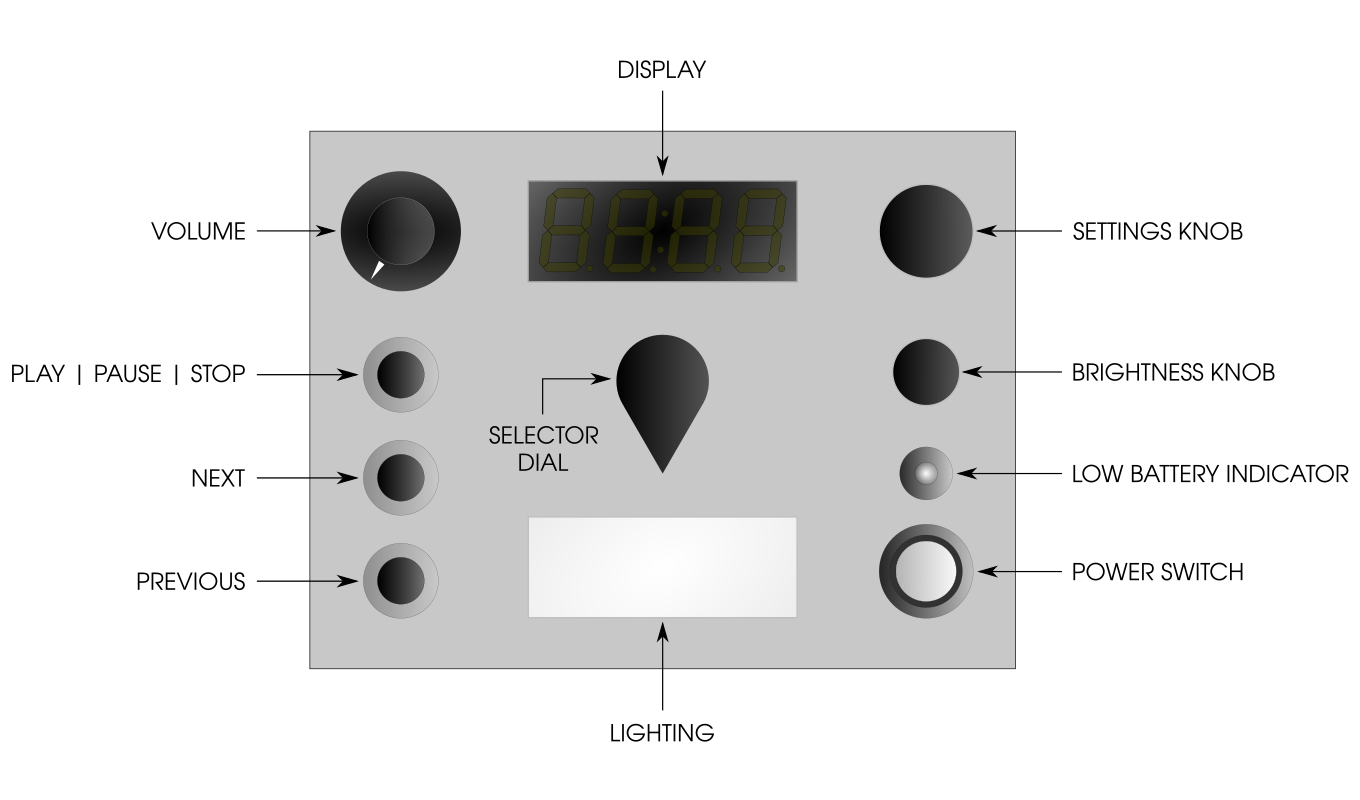
\includegraphics{images/front_panel.png}
\caption{Front}
\end{figure}

%%%%%%%%%%%%%%%%%%%%%%%%%%%%%%%%%%%%%%%%%%%%%%%%%%%%%%%%%%%%%%%%%%%%%%%%%%%%%%%%
% Front - Power
%%%%%%%%%%%%%%%%%%%%%%%%%%%%%%%%%%%%%%%%%%%%%%%%%%%%%%%%%%%%%%%%%%%%%%%%%%%%%%%%
\section{Power}

%%%%%%%%%%%%%%%%%%%%%%%%%%%%%%%%%%%%%%%%%%%%%%%%%%%%%%%%%%%%%%%%%%%%%%%%%%%%%%%%
% Front - Power - Power Switch
%%%%%%%%%%%%%%%%%%%%%%%%%%%%%%%%%%%%%%%%%%%%%%%%%%%%%%%%%%%%%%%%%%%%%%%%%%%%%%%%
\subsection{Power Switch} \label{Power Switch}

The \cPo{f} is a latching switch used to turn the device \sON{f} and \sOFF{f}.
\begin{itemize}
  \item To turn the device \sON{f}, press inward until you hear a mechanical
    click and feel it lock in place.
  \item To turn the device \sOFF{f}, press inward until you hear a mechanical
    click and feel it release.
\end{itemize}

You can visually tell whether the switch is \sON{f} or \sOFF{f} by whether or
not it is lit.\footnote{ The color of the light may vary.}

\begin{table}[H]
\ers{1}
\centering
\begin{tabu} to 7cm { X[1,c,m] X[1,c,m] }
  \sON{n} & \sOFF{n} \\
  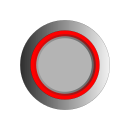
\includegraphics{images/onoff_on.png} & 
\includegraphics{images/onoff_off.png} \\
\end{tabu}
\caption{Power Switch - ON | OFF Indication}
\end{table}

It will also be flush with the bevel when \sOFF{f} and sunken in when \sON{f}.

\par\medskip

A few items of note:

\begin{itemize}
  \item When the device is plugged in there is no need to switch the device
    \sOFF{f}.
  \item To reduce power consumption when running unplugged, instead of switching
    the device \sOFF{f}, you can:
    \begin{itemize}
      \item Use the \hyperref[Brightness Knob]{\cBr{f}} to blank both the
        \hyperref[Display]{\cDi{f}} and \hyperref[Lighting]{\cLi{f}}.
      \item Use the \hyperref[Play|Pause|Stop]{\cPl{f}} push-button to \sAuSt{f}
        the \hyperref[Audio]{\mAu{f}}.
      \item Set \mPSNa{f}, \mPSSt{f} and/or \mPSSl{f} timers or forcibly put the
        device to sleep using \mPSTo{f} - see \hyperref[Power Settings]{\mPS{f}}
        for configuration and usage.
    \end{itemize}
\end{itemize}

%%%%%%%%%%%%%%%%%%%%%%%%%%%%%%%%%%%%%%%%%%%%%%%%%%%%%%%%%%%%%%%%%%%%%%%%%%%%%%%%
% Front - Power - Low Battery Indicator
%%%%%%%%%%%%%%%%%%%%%%%%%%%%%%%%%%%%%%%%%%%%%%%%%%%%%%%%%%%%%%%%%%%%%%%%%%%%%%%%
\subsection{Low Battery Indicator} \label{Low Battery Indicator}

The \cLB{f} is a red LED and is used to indicate that the device needs to be
recharged.  When the light turns on, the battery charge is getting low.

\begin{table}[H]
\ers{1}
\centering
\begin{tabu} to 6cm { X[1,c,m] X[1,c,m] }
  OK & LOW \\
  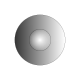
\includegraphics{images/lowbat_off.png}
    & 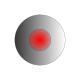
\includegraphics{images/lowbat_on.png} \\
\end{tabu}
\caption{Low Battery Indicator}
\end{table}

Note that when music is playing, the light might flicker on and off. This is
because the electric current varies a great deal when playing audio and a high
volume setting and/or certain sounds (usually low end sounds) can cause the
voltage in the circuit to temporarily drop triggering the \cLB{f}.  Turning
the volume down may get rid of the flicker.  Either way, the battery should
be recharged.

%%%%%%%%%%%%%%%%%%%%%%%%%%%%%%%%%%%%%%%%%%%%%%%%%%%%%%%%%%%%%%%%%%%%%%%%%%%%%%%%
% Front - Screens
%%%%%%%%%%%%%%%%%%%%%%%%%%%%%%%%%%%%%%%%%%%%%%%%%%%%%%%%%%%%%%%%%%%%%%%%%%%%%%%%
\section{Screens}

%%%%%%%%%%%%%%%%%%%%%%%%%%%%%%%%%%%%%%%%%%%%%%%%%%%%%%%%%%%%%%%%%%%%%%%%%%%%%%%%
% Front - Screens - Display
%%%%%%%%%%%%%%%%%%%%%%%%%%%%%%%%%%%%%%%%%%%%%%%%%%%%%%%%%%%%%%%%%%%%%%%%%%%%%%%%
\subsection{Display} \label{Display}

The \cDi{f} is the primary means of conveying information.  It is an LED
\href{https://en.wikipedia.org/wiki/Seven-segment\_display}{Seven-Segment Display}
and can display the full range of numerical digits as well as the majority of
letters.\footnote{ See \hyperref[Display Digits]{Number \& Letter Display Representations}
in the Appendix for a complete list.}  It can also display a decimal point after
each digit and a colon in the middle.

\par\medskip

The brightness of the \cDi{f} is controlled by the
\hyperref[Brightness Knob]{\cBr{f}}.

%%%%%%%%%%%%%%%%%%%%%%%%%%%%%%%%%%%%%%%%%%%%%%%%%%%%%%%%%%%%%%%%%%%%%%%%%%%%%%%%
% Front - Screens - Lighting
%%%%%%%%%%%%%%%%%%%%%%%%%%%%%%%%%%%%%%%%%%%%%%%%%%%%%%%%%%%%%%%%%%%%%%%%%%%%%%%%
\subsection{Lighting} \label{Lighting}

The \cLi{f} is made up of \num{16} RGB LEDs - 2 rows with \num{8} in each row.
A translucent white plastic called Delrin is used to diffuse the light.  Its
primary use is as a night light or timer status indicator.
See \hyperref[Clock]{\mCl{f}} and \hyperref[Timer]{\mTi{f}} respectively for
more information on its use and \hyperref[Set Night Light]{\mSN{f}} for
instructions on setting the \num{3} configurable night light colors.

\par\medskip

The brightness of the \cLi{f} window is controlled by the
\hyperref[Brightness Knob]{\cBr{f}}.

%%%%%%%%%%%%%%%%%%%%%%%%%%%%%%%%%%%%%%%%%%%%%%%%%%%%%%%%%%%%%%%%%%%%%%%%%%%%%%%%
% Front - Screens - Brightness Knob
%%%%%%%%%%%%%%%%%%%%%%%%%%%%%%%%%%%%%%%%%%%%%%%%%%%%%%%%%%%%%%%%%%%%%%%%%%%%%%%%
\subsection{Brightness Knob} \label{Brightness Knob}

The \cBr{f} is an optical rotary encoder and is used to control the brightness
of both the \hyperref[Display]{\cDi{f}} and \hyperref[Lighting]{\cLi{f}}. It
does not have start or stop positions and will turn indefinitely in either
direction.

\begin{itemize}
  \item Turn \textit{clockwise} to \textit{increase} the brightness.
  \item Turn \textit{counter-clockwise} to \textit{decrease} the
    brightness.\footnote{ The \cDi{ss} does not dim seamlessly and you will
    likely notice that it jumps or drops in brightness.  This is normal
    behavior as the hardware only supports \num{16} brightness levels.}
\end{itemize}

Continually turning in one direction or the other will eventually either:

\begin{enumerate}
  \item Reach a \textit{maximum} brightness, or
  \item Blank both the \cDi{f} and \cLi{f}.
\end{enumerate}

\info{When running on battery power and not using the \cDi{f} or \cLi{f} - for
example, if just listening to music - turn the \cBr{f} \textit{counter-clockwise}
until they go blank to prolong battery charge.}

%%%%%%%%%%%%%%%%%%%%%%%%%%%%%%%%%%%%%%%%%%%%%%%%%%%%%%%%%%%%%%%%%%%%%%%%%%%%%%%%
% Front - UI Controls
%%%%%%%%%%%%%%%%%%%%%%%%%%%%%%%%%%%%%%%%%%%%%%%%%%%%%%%%%%%%%%%%%%%%%%%%%%%%%%%%
\section{UI Controls}

The \cRs{f} and \cEs{f} are the primary controls used to interact with the
device and make use of its functionality.

%%%%%%%%%%%%%%%%%%%%%%%%%%%%%%%%%%%%%%%%%%%%%%%%%%%%%%%%%%%%%%%%%%%%%%%%%%%%%%%%
% Front - UI Controls - Selector Dial
%%%%%%%%%%%%%%%%%%%%%%%%%%%%%%%%%%%%%%%%%%%%%%%%%%%%%%%%%%%%%%%%%%%%%%%%%%%%%%%%
\subsection{Selector Dial} \label{Selector Dial}

The \cRs{f} is a \num{3} position, \num{90}° angle rotary switch and is
used to select available operational modes.

\begin{table}[H]
\ers{0.1}
\centering
\begin{tabu}{ c c c }
  \dLe{f} & \dMi{f} & \dRi{f} \\
  \sLe & \sMi & \sRi
\end{tabu}
\caption{Selector Dial Positions}
\end{table}

For information on usage, see \hyperref[Operation - Selector Dial]{\cRs{f}} in
the \hyperref[Operation]{Operation} chapter.

%%%%%%%%%%%%%%%%%%%%%%%%%%%%%%%%%%%%%%%%%%%%%%%%%%%%%%%%%%%%%%%%%%%%%%%%%%%%%%%%
% Front - UI Controls - Settings Knob
%%%%%%%%%%%%%%%%%%%%%%%%%%%%%%%%%%%%%%%%%%%%%%%%%%%%%%%%%%%%%%%%%%%%%%%%%%%%%%%%
\subsection{Settings Knob} \label{Settings Knob}

The \cEs{f} is a combination optical rotary encoder w/ detents \textit{and}
momentary switch which can be both \textit{turned} and \textit{pressed}.  It
does \textit{not} have start or stop positions and will turn indefinitely in
either direction.

\par\medskip

For information on usage, see \hyperref[Operation - Settings Knob]{\cEs{f}} in
the \hyperref[Operation]{Operation} chapter.

%%%%%%%%%%%%%%%%%%%%%%%%%%%%%%%%%%%%%%%%%%%%%%%%%%%%%%%%%%%%%%%%%%%%%%%%%%%%%%%%
% Front - Audio Controls
%%%%%%%%%%%%%%%%%%%%%%%%%%%%%%%%%%%%%%%%%%%%%%%%%%%%%%%%%%%%%%%%%%%%%%%%%%%%%%%%
\section{Audio Controls}

The left side of the front panel is devoted to the \hyperref[Audio]{\mAu{f}}.

%%%%%%%%%%%%%%%%%%%%%%%%%%%%%%%%%%%%%%%%%%%%%%%%%%%%%%%%%%%%%%%%%%%%%%%%%%%%%%%%
% Front - Audio Controls - Volume
%%%%%%%%%%%%%%%%%%%%%%%%%%%%%%%%%%%%%%%%%%%%%%%%%%%%%%%%%%%%%%%%%%%%%%%%%%%%%%%%
\subsection{Volume} \label{Volume}

The \cVo{f} knob is a dual-gang potentiometer and controls the volume level of
the \mAu{f}\footnote{ The \cVo{ss} knob is not connected to the \cBe{ss} so
cannot control its volume.} and has a \textit{white arrow} indicator on the
sleeve.  Unlike the \hyperref[Settings Knob]{\cEs{f}} and
\hyperref[Brightness Knob]{\cBr{f}} it does \textit{not} turn indefinitely and
has physical start and stop positions.

\par\medskip

For usage information, see \hyperref[Audio - Volume]{\cVo{f}} in the
\hyperref[Audio]{\mAu{f}} section.

%%%%%%%%%%%%%%%%%%%%%%%%%%%%%%%%%%%%%%%%%%%%%%%%%%%%%%%%%%%%%%%%%%%%%%%%%%%%%%%%
% Front - Audio Controls - Play|Pause|Stop
%%%%%%%%%%%%%%%%%%%%%%%%%%%%%%%%%%%%%%%%%%%%%%%%%%%%%%%%%%%%%%%%%%%%%%%%%%%%%%%%
\subsection{Play | Pause | Stop} \label{Play|Pause|Stop}

\cPl{f} is a momentary push-button and is used to \sAuPl{f}, \sAuPa{f} and
\sAuSt{f} the \mAu{f}.

\par\medskip

For usage information, see \hyperref[Audio - Play|Pause|Stop]{\cPl{f}} in the
\hyperref[Audio]{\mAu{f}} section.

%%%%%%%%%%%%%%%%%%%%%%%%%%%%%%%%%%%%%%%%%%%%%%%%%%%%%%%%%%%%%%%%%%%%%%%%%%%%%%%%
% Front - Audio Controls - Next
%%%%%%%%%%%%%%%%%%%%%%%%%%%%%%%%%%%%%%%%%%%%%%%%%%%%%%%%%%%%%%%%%%%%%%%%%%%%%%%%
\subsection{Next} \label{Next}

\cNe{f} is a momentary push-button and is used to \sAuSk{f} \textit{forward} one
or more tracks.

\par\medskip

For usage information, see \hyperref[Audio - Next]{\cNe{f}} in the
\hyperref[Audio]{\mAu{f}} section.

%%%%%%%%%%%%%%%%%%%%%%%%%%%%%%%%%%%%%%%%%%%%%%%%%%%%%%%%%%%%%%%%%%%%%%%%%%%%%%%%
% Front - Audio Controls - Previous
%%%%%%%%%%%%%%%%%%%%%%%%%%%%%%%%%%%%%%%%%%%%%%%%%%%%%%%%%%%%%%%%%%%%%%%%%%%%%%%%
\subsection{Previous} \label{Previous}

\cPr{f} is a momentary push-button and is used to \sAuSk{f} \textit{backward}
one or more tracks or \textit{rewind} the current track.

\par\medskip

For usage information, see \hyperref[Audio - Previous]{\cPr{f}} in the
\hyperref[Audio]{\mAu{f}} section.

%%%%%%%%%%%%%%%%%%%%%%%%%%%%%%%%%%%%%%%%%%%%%%%%%%%%%%%%%%%%%%%%%%%%%%%%%%%%%%%%
% Top
%%%%%%%%%%%%%%%%%%%%%%%%%%%%%%%%%%%%%%%%%%%%%%%%%%%%%%%%%%%%%%%%%%%%%%%%%%%%%%%%
\chapter{Top} \label{Top}

Attached to the underside of the \cTo{f} is a \cTS{f} and a \cCC{f} and holder.

\begin{figure}[H]
\centering
  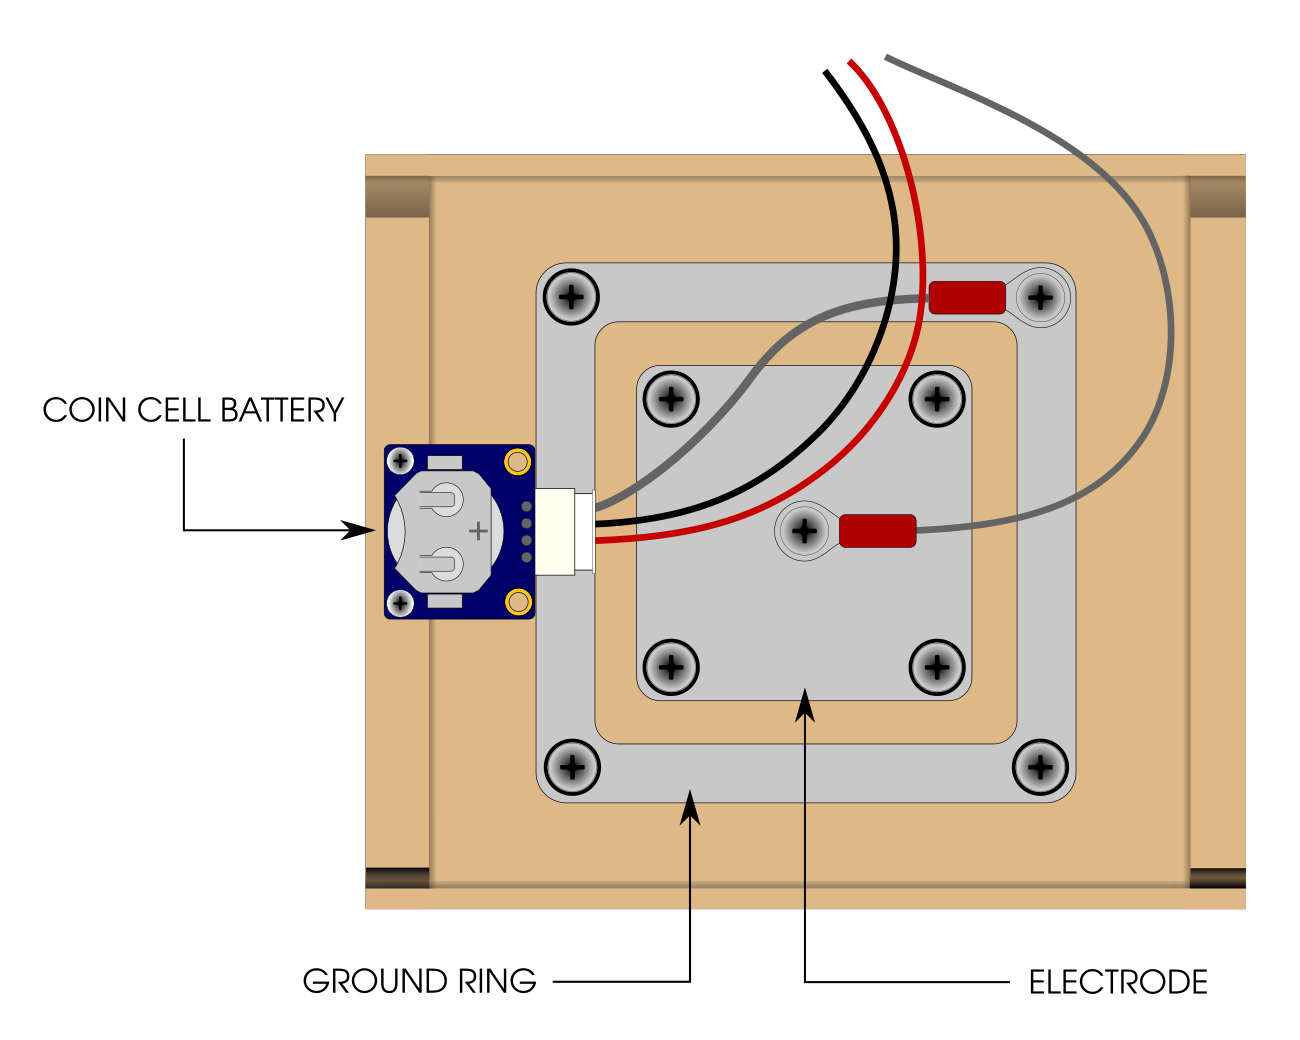
\includegraphics{images/top.png}
\caption{Top}
\end{figure}

%%%%%%%%%%%%%%%%%%%%%%%%%%%%%%%%%%%%%%%%%%%%%%%%%%%%%%%%%%%%%%%%%%%%%%%%%%%%%%%%
% Top - Touch Sensor
%%%%%%%%%%%%%%%%%%%%%%%%%%%%%%%%%%%%%%%%%%%%%%%%%%%%%%%%%%%%%%%%%%%%%%%%%%%%%%%%
\section{Touch Sensor} \label{Touch Sensor}

The \cTS{f}, also called an \textit{electrode}, is made of a \num{2$\times$2}
inch square of \mono{1/32"} thick aluminum with a wire running to the
microcontroller.  Around the electrode is an aluminum ground ring.

\par\medskip

For more information, see \hyperref[Operation - Touch Sensor]{\cTS{f}} in the
\hyperref[Operation]{Operation} chapter and \hyperref[Touch Settings]{\mTS{f}}
for how to enable and configure the touch capability of the device.

%%%%%%%%%%%%%%%%%%%%%%%%%%%%%%%%%%%%%%%%%%%%%%%%%%%%%%%%%%%%%%%%%%%%%%%%%%%%%%%%
% Top - Coin Cell Battery
%%%%%%%%%%%%%%%%%%%%%%%%%%%%%%%%%%%%%%%%%%%%%%%%%%%%%%%%%%%%%%%%%%%%%%%%%%%%%%%%
\section{Coin Cell Battery} \label{Coin Cell Battery}

The \cCC{f} is a \mono{3\thinspace V} \mono{CR2032} Lithium battery and is used
to keep the date and time updated when the device is switched \sOFF{f} via the
\hyperref[Power Switch]{\cPo{f}} and otherwise unpowered.  It is attached on the
left side just underneath the \cTo{f}.  It is \textit{not} rechargeable,
however, it should last for a number of years before needing replacement.  You
will know it needs replacing if the date and time are not correct when switching
the device \sON{f} (assuming they were correct before switching the device
\sOFF{f}).  For more information see
\hyperref[Replacing Battery]{Replacing the Coin Cell Battery}.

%%%%%%%%%%%%%%%%%%%%%%%%%%%%%%%%%%%%%%%%%%%%%%%%%%%%%%%%%%%%%%%%%%%%%%%%%%%%%%%%
% Bottom
%%%%%%%%%%%%%%%%%%%%%%%%%%%%%%%%%%%%%%%%%%%%%%%%%%%%%%%%%%%%%%%%%%%%%%%%%%%%%%%%
\chapter{Bottom} \label{Bottom}

The \cBo{f} holds and secures the \cRB{f}.

\begin{figure}[H]
\centering
  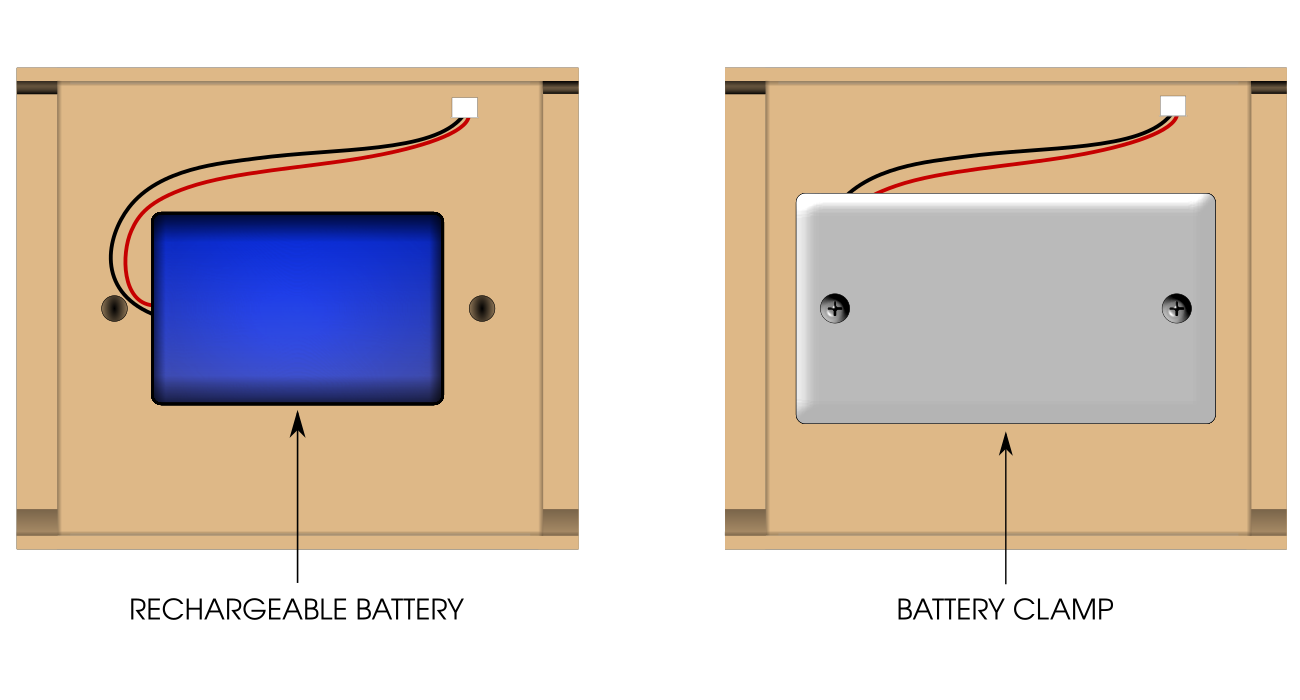
\includegraphics{images/bottom.png}
\caption{Bottom}
\end{figure}

%%%%%%%%%%%%%%%%%%%%%%%%%%%%%%%%%%%%%%%%%%%%%%%%%%%%%%%%%%%%%%%%%%%%%%%%%%%%%%%%
% Bottom - Rechargeable Battery
%%%%%%%%%%%%%%%%%%%%%%%%%%%%%%%%%%%%%%%%%%%%%%%%%%%%%%%%%%%%%%%%%%%%%%%%%%%%%%%%
\section{Rechargeable Battery} \label{Rechargeable Battery}

The \cRB{f} is a nominal \mono{3.7\thinspace V}, \mono{6600\thinspace mAh}
Lithium Ion battery pack.  It is the primary power source when the device is
unplugged and switched \sON{f}.  With music playing, the charge should last
about a day.

%%%%%%%%%%%%%%%%%%%%%%%%%%%%%%%%%%%%%%%%%%%%%%%%%%%%%%%%%%%%%%%%%%%%%%%%%%%%%%%%
% Sides
%%%%%%%%%%%%%%%%%%%%%%%%%%%%%%%%%%%%%%%%%%%%%%%%%%%%%%%%%%%%%%%%%%%%%%%%%%%%%%%%
\chapter{Sides} \label{Sides}

The \cSi{f} house the speakers and are where the screws that secure the
enclosure are.

\begin{figure}[H]
\centering
  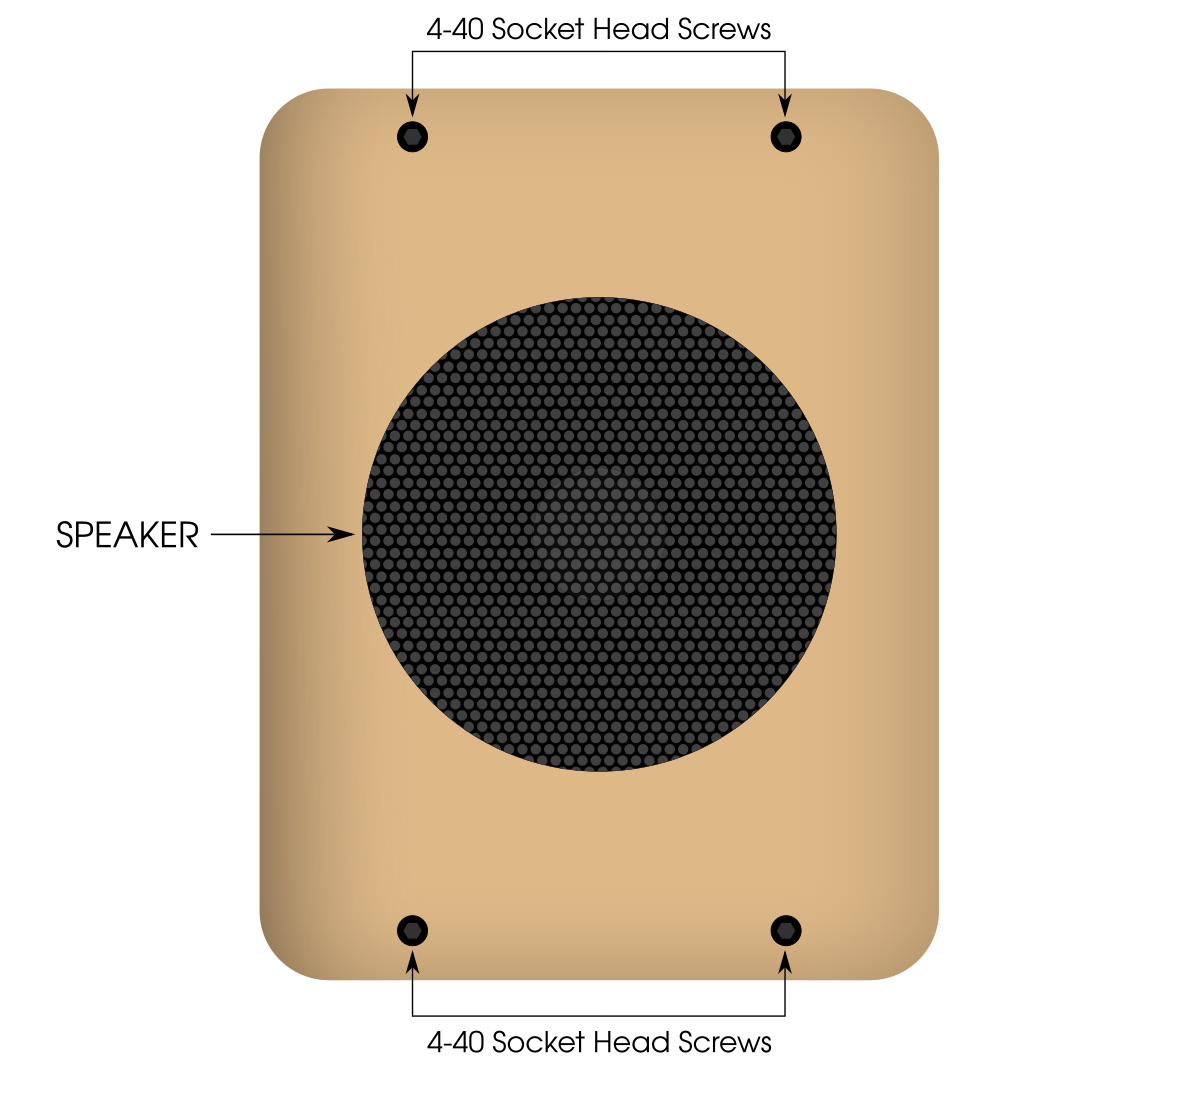
\includegraphics{images/side.png}
\caption{Side}
\end{figure}

%%%%%%%%%%%%%%%%%%%%%%%%%%%%%%%%%%%%%%%%%%%%%%%%%%%%%%%%%%%%%%%%%%%%%%%%%%%%%%%%
% Sides - Speakers
%%%%%%%%%%%%%%%%%%%%%%%%%%%%%%%%%%%%%%%%%%%%%%%%%%%%%%%%%%%%%%%%%%%%%%%%%%%%%%%%
\section{Speakers} \label{Speakers}

The \num{2} speakers, one on each side, are \mono{8\thinspace\small{$\Omega$}},
\mono{2\thinspace W}, \mono{99\thinspace dB} with paper cone and ferrite magnet.
They are used in conjunction with the \hyperref[Audio]{\mAu{f}}.  The grills are
made of \mono{1/32"} inch, \num{24} gauge perforated \num{304} stainless steel,
painted black.

%%%%%%%%%%%%%%%%%%%%%%%%%%%%%%%%%%%%%%%%%%%%%%%%%%%%%%%%%%%%%%%%%%%%%%%%%%%%%%%%
% Sides - Fastening Screws
%%%%%%%%%%%%%%%%%%%%%%%%%%%%%%%%%%%%%%%%%%%%%%%%%%%%%%%%%%%%%%%%%%%%%%%%%%%%%%%%
\section{Fastening Screws} \label{Fastening Screws}

The screws used to keep the enclosure together are \mono{4-40} Socket Head
screws made of Black-Oxide Alloy Steel and have a \mono{3/32"} hex wrench drive
size.  There are a total of \num{8} screws with \num{4} on each side.

\warning{Before taking the enclosure apart, please refer to
\hyperref[Disassembly]{Disassembly}.}

%%%%%%%%%%%%%%%%%%%%%%%%%%%%%%%%%%%%%%%%%%%%%%%%%%%%%%%%%%%%%%%%%%%%%%%%%%%%%%%%
% Back
%%%%%%%%%%%%%%%%%%%%%%%%%%%%%%%%%%%%%%%%%%%%%%%%%%%%%%%%%%%%%%%%%%%%%%%%%%%%%%%%
\chapter{Back} \label{Back}

On the \cBa{f} of the device is the \cPP{f} that is used to both power the
device and charge the \hyperref[Rechargeable Battery]{\cRB{f}} inside.

\begin{figure}[H]
\centering
  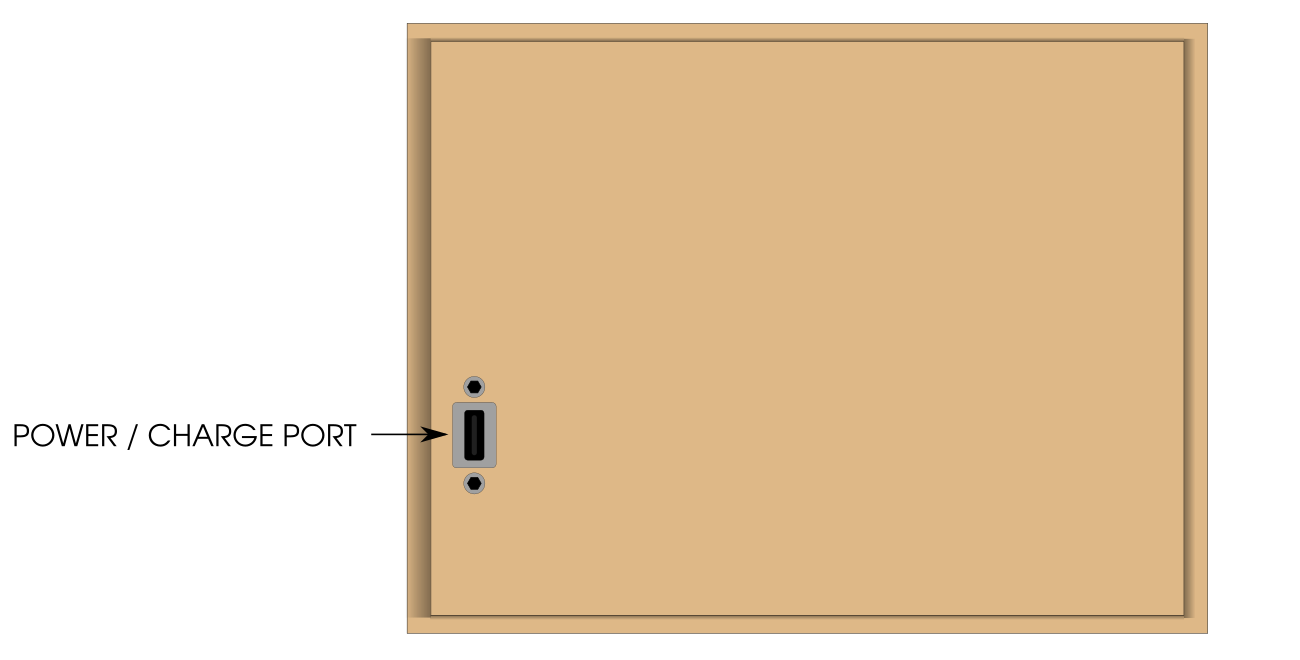
\includegraphics{images/back.png}
\caption{Back}
\end{figure}

The main circuit board is attached on the inside.  Of interest are
the \cBe{f} and removable \cMSD{f}.

\begin{figure}[H]
\centering
  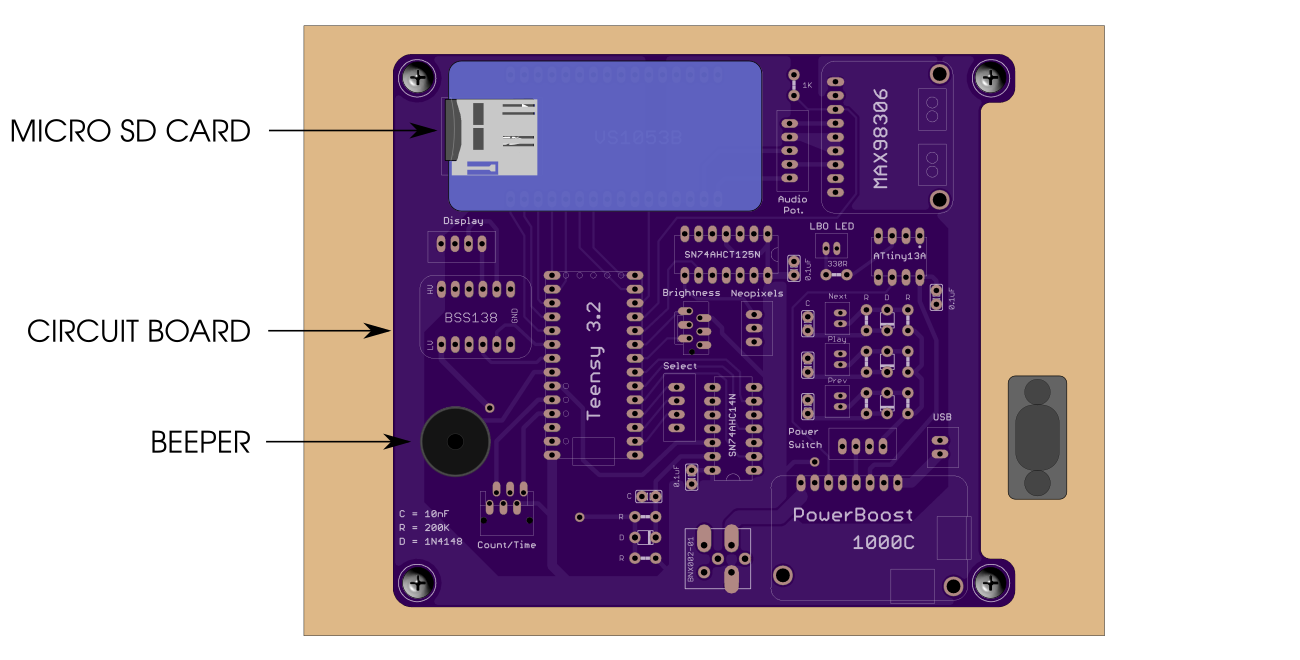
\includegraphics{images/back_circuit_board.png}
\caption{Back - Circuit Board}
\end{figure}

%%%%%%%%%%%%%%%%%%%%%%%%%%%%%%%%%%%%%%%%%%%%%%%%%%%%%%%%%%%%%%%%%%%%%%%%%%%%%%%%
% Back - Power / Charge Port
%%%%%%%%%%%%%%%%%%%%%%%%%%%%%%%%%%%%%%%%%%%%%%%%%%%%%%%%%%%%%%%%%%%%%%%%%%%%%%%%
\section{Power / Charge Port} \label{Power Port}

The \cPP{f} is a \cUSB{f} port.

\par\medskip

A few items of note:

\begin{itemize}
  \item The device can be \sON{f} or \sOFF{f} when plugging or unplugging the
    \hyperref[Power Adapter]{\cPA{f}} or other USB cable.
  \item The device can be \sON{f} or \sOFF{f} while charging.
  \item The device is fully functional while charging.
  \item The device never has to be unplugged.
\end{itemize}

See \hyperref[Powering and Recharging]{Powering \& Recharging} for more
information.

%%%%%%%%%%%%%%%%%%%%%%%%%%%%%%%%%%%%%%%%%%%%%%%%%%%%%%%%%%%%%%%%%%%%%%%%%%%%%%%%
% Back - Beeper
%%%%%%%%%%%%%%%%%%%%%%%%%%%%%%%%%%%%%%%%%%%%%%%%%%%%%%%%%%%%%%%%%%%%%%%%%%%%%%%%
\section{Beeper} \label{Beeper}

The \cBe{f} is a \mono{2.3\thinspace kHz} magnetic single tone buzzer and is
used with the \hyperref[Alarm]{\mAl{f}}, \hyperref[Timer]{\mTi{f}} and
\hyperref[Touch Settings]{\mTS{f}}.  Note, it will always sound at the same
volume since the \cVo{f} control is not connected to it and can \textit{not}
adjust it.

\par\medskip

There are two symbols used to reference the \cBe{f} that are used in later
sections.

\begin{table}[H]
\ers{2}
\centering
\begin{tabu}{X[1,c,m] | X[5,l,m]}
  \thrule
  \thbi{Symbol} & \thbi{Meaning} \\ \mrule
  \sBe & The \cBe{f} is making sound, i.e. beeping. \\ \drule{2}
  \sNBe & The \cBe{f} is mute, i.e. \textit{not} beeping. \\
  \bhrule
\end{tabu}
\end{table}

%%%%%%%%%%%%%%%%%%%%%%%%%%%%%%%%%%%%%%%%%%%%%%%%%%%%%%%%%%%%%%%%%%%%%%%%%%%%%%%%
% Back - Micro SD Card
%%%%%%%%%%%%%%%%%%%%%%%%%%%%%%%%%%%%%%%%%%%%%%%%%%%%%%%%%%%%%%%%%%%%%%%%%%%%%%%%
\section{Micro SD Card} \label{Micro SD Card}

The \cMSD{f} is used as storage for the songs on the device.  The \cMSD{f} that
comes preinstalled with the device has a read speed of at least
\num{90} \mono{MB/sec} and is formatted with the \mono{FAT32} filesystem using
\num{512} bytes per sector.

%%%%%%%%%%%%%%%%%%%%%%%%%%%%%%%%%%%%%%%%%%%%%%%%%%%%%%%%%%%%%%%%%%%%%%%%%%%%%%%%
% Accessories
%%%%%%%%%%%%%%%%%%%%%%%%%%%%%%%%%%%%%%%%%%%%%%%%%%%%%%%%%%%%%%%%%%%%%%%%%%%%%%%%
\chapter{Accessories} \label{Accessories}

%%%%%%%%%%%%%%%%%%%%%%%%%%%%%%%%%%%%%%%%%%%%%%%%%%%%%%%%%%%%%%%%%%%%%%%%%%%%%%%%
% Accessories - Power Adapter
%%%%%%%%%%%%%%%%%%%%%%%%%%%%%%%%%%%%%%%%%%%%%%%%%%%%%%%%%%%%%%%%%%%%%%%%%%%%%%%%
\section{Power Adapter} \label{Power Adapter}

The one accessory included is the \cPA{f} that is used to both power the device
and charge the \hyperref[Rechargeable Battery]{\cRB{f}}.  It is a
\mono{5.25\thinspace V}, \mono{2.4\thinspace A} switching AC/DC power adapter
that terminates with a \cUSB{f} connector that plugs into the
\hyperref[Power Port]{\cPP{f}}.  It can accept either \num{110} or \num{240}
\mono{VAC} mains so works in the US as well as other countries.

\par\medskip

If this needs to be replaced, the replacement \textit{must} be a
\mono{5\thinspace V} AC/DC adapter (or \mono{5.25\thinspace V} if you can find
one).

\danger{An adapter that is \mono{6\thinspace V}, \mono{9\thinspace V},
\mono{12\thinspace V} or above \textit{will} damage the device.}

\warning{An adapter that is less than \mono{5\thinspace V} will not be able to
power the device and it \textit{will} malfunction.}

The adapter should be rated for at least \mono{1\thinspace A} and no more than
\mono{2.5\thinspace A}.

%%%%%%%%%%%%%%%%%%%%%%%%%%%%%%%%%%%%%%%%%%%%%%%%%%%%%%%%%%%%%%%%%%%%%%%%%%%%%%%%
% Powering & Recharging
%%%%%%%%%%%%%%%%%%%%%%%%%%%%%%%%%%%%%%%%%%%%%%%%%%%%%%%%%%%%%%%%%%%%%%%%%%%%%%%%
\chapter{Powering \& Recharging} \label{Powering and Recharging}

The device can be both powered and charged using either the supplied
\hyperref[Power Adapter]{\cPA{f}} or a \textit{USB 2.0 Standard Type-A Male to
Micro Type-B Male} cable.

\par\medskip

\cUSB{f} is asymmetric and can only be plugged in one way.

\begin{figure}[H]
\centering
  
\includegraphics{images/usb.png}
\caption{USB 2.0 Micro-B}
\end{figure}

The figure below indicates how the USB 2.0 Micro-B plug should be oriented when
\textit{facing} the \hyperref[Power Port]{\cPP{f}}.

\begin{figure}[H]
\centering
  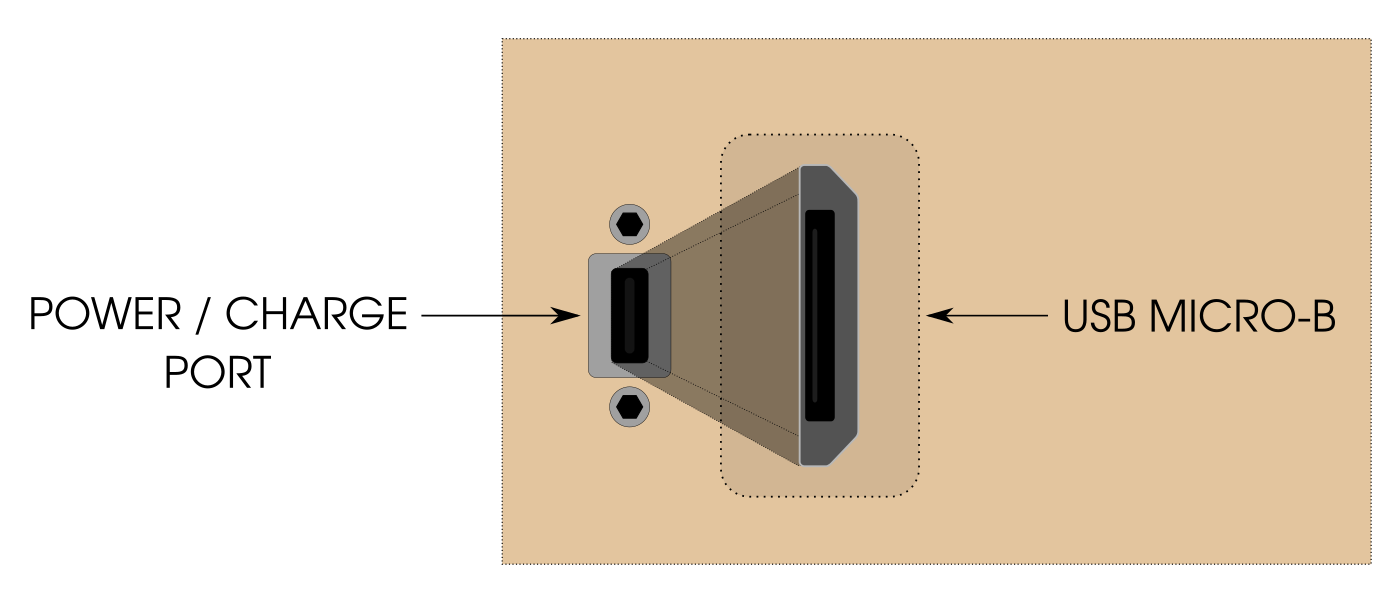
\includegraphics{images/usb_orientation.png}
\caption{USB 2.0 Micro-B $\longrightarrow$ Power / Charge Port Orientation}
\end{figure}

Using the supplied \cPA{f}, plug the \cUSB{f} end into the \cPP{f} on the
\cBa{f} of the device and the 2-prong end into a wall or power strip receptacle.

\par\medskip

If a \textit{USB 2.0 Standard Type-A Male to Micro Type-B Male} cable is used,
connect the Micro-B end into the \cPP{f} and the Standard Type-A end into the
USB port on a computer or USB hub.

%%%%%%%%%%%%%%%%%%%%%%%%%%%%%%%%%%%%%%%%%%%%%%%%%%%%%%%%%%%%%%%%%%%%%%%%%%%%%%%%
% Powering & Recharging - Recharging
%%%%%%%%%%%%%%%%%%%%%%%%%%%%%%%%%%%%%%%%%%%%%%%%%%%%%%%%%%%%%%%%%%%%%%%%%%%%%%%%
\section{Recharging} \label{Recharging}

The \hyperref[Low Battery Indicator]{\cLB{f}} will light up when the device
needs to be recharged.  Unfortunately there is no way to indicate that the
battery has finished charging. Using the supplied
\hyperref[Power Adapter]{\cPA{f}}, it should take about \num{8} hours to charge
if the \cLB{f} is signaling - plug it in before going to bed and it should be
charged by the time you wake up.  When using a \textit{USB 2.0 Standard Type-A
Male to Micro Type-B Male} cable, charging may take longer since USB ports on a
computer generally do not supply as much current as the \cPA{f} will.



%%%%%%%%%%%%%%%%%%%%%%%%%%%%%%%%%%%%%%%%%%%%%%%%%%%%%%%%%%%%%%%%%%%%%%%%%%%%%%%%
% Operation
%%%%%%%%%%%%%%%%%%%%%%%%%%%%%%%%%%%%%%%%%%%%%%%%%%%%%%%%%%%%%%%%%%%%%%%%%%%%%%%%
%%%%%%%%%%%%%%%%%%%%%%%%%%%%%%%%%%%%%%%%%%%%%%%%%%%%%%%%%%%%%%%%%%%%%%%%%%%%%%%%
% Operation
%%%%%%%%%%%%%%%%%%%%%%%%%%%%%%%%%%%%%%%%%%%%%%%%%%%%%%%%%%%%%%%%%%%%%%%%%%%%%%%%
\part{Operation} \label{Operation}

%%%%%%%%%%%%%%%%%%%%%%%%%%%%%%%%%%%%%%%%%%%%%%%%%%%%%%%%%%%%%%%%%%%%%%%%%%%%%%%%
% Modules
%%%%%%%%%%%%%%%%%%%%%%%%%%%%%%%%%%%%%%%%%%%%%%%%%%%%%%%%%%%%%%%%%%%%%%%%%%%%%%%%
\chapter{Modules} \label{Modules}

%%%%%%%%%%%%%%%%%%%%%%%%%%%%%%%%%%%%%%%%%%%%%%%%%%%%%%%%%%%%%%%%%%%%%%%%%%%%%%%%
% Modules - Introduction
%%%%%%%%%%%%%%%%%%%%%%%%%%%%%%%%%%%%%%%%%%%%%%%%%%%%%%%%%%%%%%%%%%%%%%%%%%%%%%%%
\section{Introduction}

There are a number of functions that the device performs.  Each set of
functionality will be called a \textit{module}.  There are some modules that are
always active and some that can only be active at one time.  Those that are
always active will be called \textit{components}.  Those that can only be active
at one time will be called \textit{modes}.

\begin{table}[H]
\ers{1}
\centering
\begin{tabu} { X[1,c,m] | X[1,c,m] }
  \thrule

  & \hyperref[Audio]{\mAu{s}} \\
  \thbi{Components} & \hyperref[Alarm]{\mAl{s}} \\
  & \hyperref[Power]{\mPo{s}} \\ \mrule

  & \hyperref[Clock]{\mCl{s}} \\
  & \hyperref[Set Alarm]{\mSA{s}}  \\
  & \hyperref[Timer]{\mTi{s}} \\
  \thbi{Modes} & \hyperref[Set Clock]{\mSC{s}} \\
  & \hyperref[Power Settings]{\mPS{s}} \\
  & \hyperref[Touch Settings]{\mTS{s}} \\
  & \hyperref[Set Night Light]{\mSN{s}} \\
  \bhrule
\end{tabu}
\caption {Modules}
\end{table}

%%%%%%%%%%%%%%%%%%%%%%%%%%%%%%%%%%%%%%%%%%%%%%%%%%%%%%%%%%%%%%%%%%%%%%%%%%%%%%%%
% Modules - State Diagrams
%%%%%%%%%%%%%%%%%%%%%%%%%%%%%%%%%%%%%%%%%%%%%%%%%%%%%%%%%%%%%%%%%%%%%%%%%%%%%%%%
\section{State Diagrams}

At the end of each module section will be a diagram showing the states it can be
in and the movement from one state to another and actions triggering the
movement.  The following table shows and describes the diagram elements.

\pagebreak

\ers{3}
\begin{longtabu}{ X[1,c,m] | X[5,l,m] }
  \thrule

  \thbi{Symbol} & \thbi{Meaning} \\ \mdrule

  \symMode{MODULE}
    & An element that is a \mode{sym}{MODULE}, i.e. a \mode{sym}{MODE}
      or \mode{sym}{COMPONENT}. \\ \mrule

  \symMenu{MENU}
    & An element that is a \menu{sym}{MENU} option available in certain modes.
      A menu state will contain a number options that will branch
      to different states. \\ \mrule

  \symState{STATE}
    & An element that is a \state{sym}{STATE} that a mode or
      component can be in. \\ \mrule

  \multirow{6}{*}{\symUnidirectional}
    & A \textit{unidirectional} or one-way path or flow from one element to
      the same or different element. \\ \dcrule{2}{2}
    & \parbox{\linewidth}{\centering \symUniModule \quad\quad \symUniMenu \quad\quad \symUniState} \\
    & \footnotesize{One or more actions may be associated
        with the path, i.e. will trigger the movement from one element
        to another. Either a symbol or text may be located next to or near
        the path line indicating the
        action that triggers the movement.} \\
    & \parbox{\linewidth}{\centering \symUniStateAction} \\ \dcrule{2}{2}
    & \footnotesize{A state can have a path that points to itself.
        There may be output or effects due to the action but
        the state does not change.} \\
    & \parbox{0.85\linewidth}{\centering \symUniSameState} \strut \\ \mrule

  \multirow{5}{*}{\symBidirectional}
    & A \textit{bidirectional} or two-way path or flow between two elements. \\ \dcrule{2}{2}
    & \footnotesize{One or more actions may be associated
        with the path, i.e will trigger the movement between the two
        elements. Either an action
        symbol or text will be located next to or near the path line
        indicating the action that triggers the movement.} \\
    & \parbox{\linewidth}{\centering \symBiStateOne} \\ \dcrule{2}{2}
    & \footnotesize{If there is more than one action associated
        with the path, the action \textit{nearest the arrow} is
        what determines the path or flow \textit{in the direction of the arrow}.} \\
    & \parbox{\linewidth}{\centering \symBiState} \\ \mrule

  \pagebreak
  \mrule

  \multirow{3}{*}{\symNode}
    & A \textit{node} that combines two or more unidirectional paths from two or
      more states into one unidirectional path to one state. \\ \dcrule{2}{2}
    & \footnotesize{Each path leading into the node will have an
        action associated with it.  The actions may be the same
        or different, but the resulting state will be the same.} \\
    & \parbox{\linewidth}{\centering \symNodeState} \strut \\

  \bhrule
\caption{State Diagram Symbols}
\end{longtabu}

%%%%%%%%%%%%%%%%%%%%%%%%%%%%%%%%%%%%%%%%%%%%%%%%%%%%%%%%%%%%%%%%%%%%%%%%%%%%%%%%
% Modules - Components
%%%%%%%%%%%%%%%%%%%%%%%%%%%%%%%%%%%%%%%%%%%%%%%%%%%%%%%%%%%%%%%%%%%%%%%%%%%%%%%%
\section{Components}

Components run and function concurrently and independent of any \textit{mode}
the device might be in.

\par\medskip

There are \num{3} components each described in individual sections.

\begin{table}[H]
\ers{4}
\centering
\begin{tabu}{ X[1,c,m] | X[3,l,m] }
  \thrule
  \thbi{Component} & \thbi{Description} \\ \mrule

  \hyperref[Audio]{\mAu{s}}
    & Provides the functionality related to track selection and
      playback. \\ \drule{2}
  \hyperref[Alarm]{\mAl{s}}
    & Contains the functionality related to alarm waking, snoozing and stopping
      and remains active in all power states. \\ \drule{2}
  \hyperref[Power]{\mPo{s}}
    & Governs device power states and when the device should nap, sleep or
      auto-stop the audio. \\
  \bhrule
\end{tabu}
\end{table}

%%%%%%%%%%%%%%%%%%%%%%%%%%%%%%%%%%%%%%%%%%%%%%%%%%%%%%%%%%%%%%%%%%%%%%%%%%%%%%%%
% Modules - Modes
%%%%%%%%%%%%%%%%%%%%%%%%%%%%%%%%%%%%%%%%%%%%%%%%%%%%%%%%%%%%%%%%%%%%%%%%%%%%%%%%
\section{Modes}

A mode is a device state containing specific functionality.  The device can be
in \textit{one and only one} mode at a time.  There are \num{7} modes each
described in individual sections.

\begin{table}[H]
\ers{4}
\centering
\begin{tabu}{ X[1,c,m] | X[3,l,m] }
  \thrule
  \thbi{Mode} & \thbi{Description} \\ \mrule

  \hyperref[Clock]{\mCl{s}}
    & Displays the time. Can display the date and current track.
    Provides direct selection of a track for playback. Is the only mode
    where the night light can be turned on and off. \\ \drule{2}
  \hyperref[Set Alarm]{\mSA{s}} & Set a time of day alarm that is used by
    the \hyperref[Alarm]{\mAl{s}} component. \\ \drule{2}
  \hyperref[Timer]{\mTi{s}} & Set and run a timer. \\ \drule{2}
  \hyperref[Set Clock]{\mSC{s}} & Set the time and date. \\ \drule{2}
  \hyperref[Power Settings]{\mPS{s}} & Settings related to power consumption
    that are used by the \hyperref[Power]{\mPo{s}} component. \\ \drule{2}
  \hyperref[Touch Settings]{\mTS{s}} & Settings related to the touch sensing
    capability of the device. \\ \drule{2}
  \hyperref[Set Night Light]{\mSN{s}} & Set any of the \num{3} configurable
    night light colors. \\

  \bhrule
\end{tabu}
\end{table}

Modes are selected using the \cRs{f} and the \cEs{f}.  They are partitioned
into \mPr{f}, \mSe{f} and \mTe{f}.

\begin{table}[H]
\ers{1}
\centering
\begin{tabu} { X[1,c,m] | X[1,c,m] }
  \thrule

  & \hyperref[Clock]{\mCl{s}} \\
  \hyperref[Primary Modes]{\mPr{s}} & \hyperref[Set Alarm]{\mSA{s}} \\
  & \hyperref[Timer]{\mTi{s}} \\ \mrule

  \multirow{2}{*}[-1mm]{\hyperref[Secondary Modes]{\mSe{s}}}
    & \hyperref[Set Clock]{\mSC{s}} \\
  & \hyperref[Power Settings]{\mPS{s}} \\ \mrule

  \multirow{2}{*}[-1mm]{\hyperref[Tertiary Modes]{\mTe{s}}}
    & \hyperref[Touch Settings]{\mTS{s}} \\
  & \hyperref[Set Night Light]{\mSN{s}} \\
  \bhrule
\end{tabu}
\caption {Modes}
\end{table}

The position of the \cRs{f} avails a subset of modes.  When the \cRs{f} is
turned, the \mPr{f} mode is automatically selected.  The \cEs{f} is then used
to select \mSe{f} and \mTe{f} modes.

%%%%%%%%%%%%%%%%%%%%%%%%%%%%%%%%%%%%%%%%%%%%%%%%%%%%%%%%%%%%%%%%%%%%%%%%%%%%%%%%
% Modules - Modes - Settings Modes
%%%%%%%%%%%%%%%%%%%%%%%%%%%%%%%%%%%%%%%%%%%%%%%%%%%%%%%%%%%%%%%%%%%%%%%%%%%%%%%%
\subsection{Settings Modes}

Settings that can change value will, in general, be \textit{blinking} on the
\cDi{f}. If there is more than one setting to configure on the \cDi{f} at a time,
as in the case of setting a time (hour and minute) or date (month and day), the
current setting will be \textit{blinking}.

%%%%%%%%%%%%%%%%%%%%%%%%%%%%%%%%%%%%%%%%%%%%%%%%%%%%%%%%%%%%%%%%%%%%%%%%%%%%%%%%
% Modules - Modes - Modes Diagram
%%%%%%%%%%%%%%%%%%%%%%%%%%%%%%%%%%%%%%%%%%%%%%%%%%%%%%%%%%%%%%%%%%%%%%%%%%%%%%%%
\subsection{Modes Diagram}

The following diagram illustrates the modes of operation and the actions using
the \cRs{f} and \cEs{f} that lead to and from each mode.

\begin{figure}[H]
\centering
  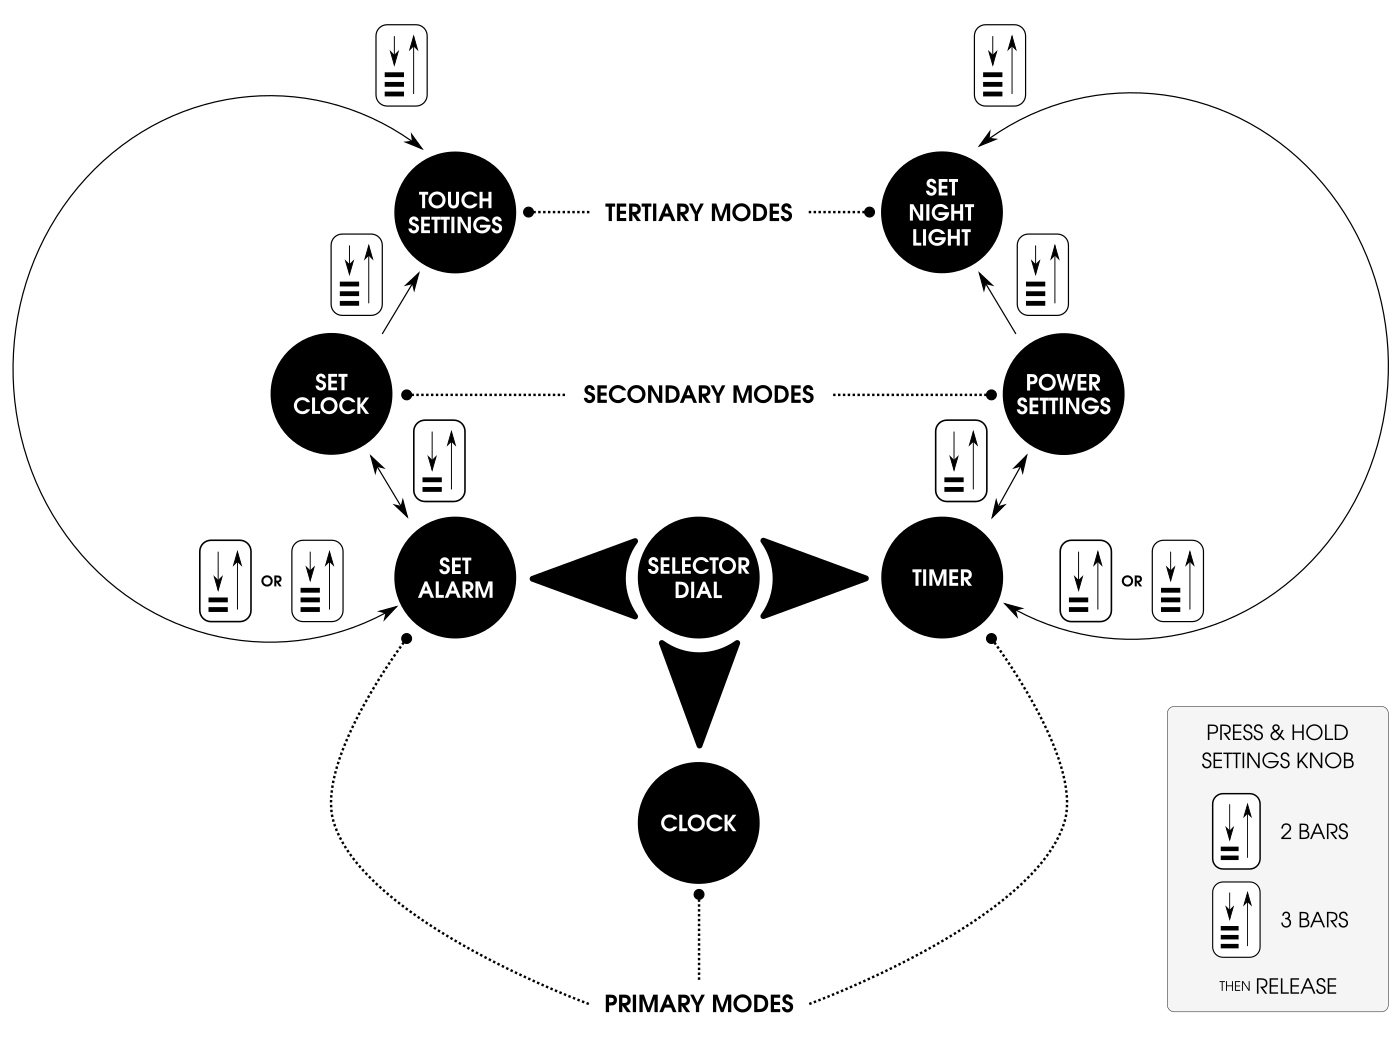
\includegraphics{images/modes_diagram.png}
\caption{Modes Diagram}
\end{figure}

%%%%%%%%%%%%%%%%%%%%%%%%%%%%%%%%%%%%%%%%%%%%%%%%%%%%%%%%%%%%%%%%%%%%%%%%%%%%%%%%
% Selector Dial
%%%%%%%%%%%%%%%%%%%%%%%%%%%%%%%%%%%%%%%%%%%%%%%%%%%%%%%%%%%%%%%%%%%%%%%%%%%%%%%%
\chapter{Selector Dial} \label{Operation - Selector Dial}

The \cRs{f} is used to select a subset of available modes.  The position
determines which modes are available.

\begin{table}[H]
\ers{2}
  \begin{tabu}{ X[1,c,m] | X[1,c,m] | X[1,c,m] | X[1,c,m] }  
    \thrule
    \multirow{2}{*}[-1mm]{\thbi{Position}}
      & \multicolumn{3}{c}{\thbi{Modes}} \\ \tabucline{2-4}

    & \mPr{n} & \mSe{n} & \mTe{n}
    \\ \hline

    \sLe & \hyperref[Set Alarm]{\mSA{s}}
      & \hyperref[Set Clock]{\mSC{s}}
      & \hyperref[Touch Settings]{\mTS{s}} \\ \drule{4}
    \sMi & \hyperref[Clock]{\mCl{s}} & --- & --- \\ \drule{4}
    \sRi & \hyperref[Timer]{\mTi{s}}
      & \hyperref[Power Settings]{\mPS{s}}
      & \hyperref[Set Night Light]{\mSN{s}} \\
  \bhrule
  \end{tabu}
\caption {Selector Dial - Positions \& Modes}
\end{table}

Turning the \cRs{f} will automatically set the mode to the \mPr{f} mode for the
given position.  The \hyperref[Operation - Settings Knob]{\cEs{f}} is then used
to select \mSe{f} and \mTe{f} modes.

\par\medskip

There are a number of symbols used to indicate turning actions.

\begin{table}[H]
\ers{5}
\centering
  \begin{tabu} { X[1,c,m] | X[3,l,m] }
    \thrule
    \thbi{Symbol} & \thbi{Meaning} \\ \mrule
    $\hskip -5.5mm$ \sMtoL & Turn from \dMi{f} to \dLe{f}. \\ \drule{2}
    $\hskip -5.5mm$ \sLtoM & Turn from \dLe{f} to \dMi{f}. \\ \drule{2}
    $\hskip 2.5mm$ \sMtoR & Turn from \dMi{f} to \dRi{f}. \\ \drule{2}
    $\hskip 2.5mm$ \sRtoM & Turn from \dRi{f} to \dMi{f}. \\ \drule{2}
    \sLtoR & Turn from \dLe{f} to \dRi{f}. \\ \drule{2}
    \sRtoL & Turn from \dRi{f} to \dLe{f}. \\
    \bhrule
  \end{tabu}
\caption {Selector Dial - Symbols}
\end{table}

%%%%%%%%%%%%%%%%%%%%%%%%%%%%%%%%%%%%%%%%%%%%%%%%%%%%%%%%%%%%%%%%%%%%%%%%%%%%%%%%
% Settings Knob
%%%%%%%%%%%%%%%%%%%%%%%%%%%%%%%%%%%%%%%%%%%%%%%%%%%%%%%%%%%%%%%%%%%%%%%%%%%%%%%%
\chapter{Settings Knob} \label{Operation - Settings Knob}

The \cEs{f} is the primary control for interacting with the device.  It can be
\textit{turned} and \textit{pressed}.

%%%%%%%%%%%%%%%%%%%%%%%%%%%%%%%%%%%%%%%%%%%%%%%%%%%%%%%%%%%%%%%%%%%%%%%%%%%%%%%%
% Settings Knob - Turning
%%%%%%%%%%%%%%%%%%%%%%%%%%%%%%%%%%%%%%%%%%%%%%%%%%%%%%%%%%%%%%%%%%%%%%%%%%%%%%%%
\section{Turning}

There are \textit{no} start or stop positions when turning and it will turn
indefinitely in either direction.  While turning, you will notice bumps - termed
\textit{detents} - that provide a tactile feel for turning progression.

\par\medskip

In general, when setting values:

\begin{itemize}
  \item Turning \textit{clockwise} will \textit{increase} a value.
  \item Turning \textit{counter-clockwise} will \textit{decrease} a value.
  \item Values will \textit{change} at each \textit{detent}.
\end{itemize}

If you turn past a \textit{minimum} or \textit{maximum}, the value will usually
wrap or cycle.

\begin{itemize}
  \item If a value is at a \textit{maximum}, a \textit{clockwise} turn will
    circle to the \textit{minimum}.
  \item If a value is at a \textit{minimum}, a \textit{counter-clockwise} turn
    will circle to the \textit{maximum}.
\end{itemize}

\begin{figure}[H]
\centering
  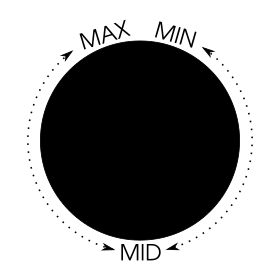
\includegraphics{images/settings_knob_wrap.png}
\caption{Settings Knob - Turning}
\end{figure}

Note that the above figure is not a literal representation of where values will
lie in relation to the \cEs{f}.  You may have to turn the knob for only a couple
of detents to reach a midpoint value or cycle through all of the allowable
values.  Or you may have to turn for many revolutions.  It is meant to show that
values are arranged circularly as opposed to linearly.

\par\medskip

Consider, for example, setting a minute or second value, where the allowable
range is \mono{0-59}.  If the current value is \num{59}, a clockwise turn will
cycle to \num{0}.  Likewise if the current value is \num{0}, a counter-clockwise
turn will cycle to \num{59}.

\begin{figure}[H]
\centering
  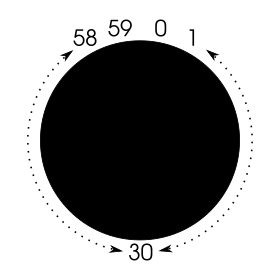
\includegraphics{images/settings_knob_wrap_example.png}
\end{figure}

\info{It can often be quicker to turn in the opposite direction to get to a
value.}

\par\medskip

There are a number of symbols that will be used indicating direction, number of
times, not to turn or a failure to turn within a specified amount of time.

\begin{table}[H]
\ers{2}
\centering
  \begin{tabu}{ X[1,c,m] | X[4,l,m] }
  \thrule

  \thbi{Symbol} & \thbi{Meaning} \\ \mrule

  \sTu & Turn in \textit{any} direction. \\ \drule{2}
  \sCl & Turn \textit{clockwise}. \\ \drule{2}
  \sCC & Turn \textit{counter-clockwise}. \\ \drule{2}
  \multirow{2}{*}[-1mm]{$\hskip 3.3mm$ \sTuN{$N$}}
    & Turn for at least $N$ detents in any direction. \\
  & \quad \sTuN{3} $\longrightarrow$ Turn until at least \num{3} detents
    are felt. \\ \drule{2}
  \multirow{2}{*}[-1mm]{$\hskip 3.3mm$ \sTuN{$N$s}} & Turn \textit{within}
    $N$ seconds. \\
  & \quad \sTuN{3s} $\longrightarrow$ Turn within \num{3} seconds. \\ \drule{2}
  \sNTu & Do \textit{not} turn. \\ \drule{2}
  \multirow{2}{*}[-1mm]{$\hskip 4.4mm$ \sNTuN{$N$}} & Failure to turn
    \textit{within} $N$ seconds. \\
  & \quad \sNTuN{15} $\longrightarrow$ Failure to turn within \num{15}
    seconds. \\
  \bhrule
  \end{tabu}
\caption{Settings Knob - Turn Symbols}
\end{table}

When the \cEs{f} is turned, you will feel bumps.  These are called
\textit{detents}.  When it is specified to turn $N$ times, it means detents
and \textit{not} full rotations.  So \enspace \sTuN{3} means to turn for at
least \num{3} bumps/detents.

%%%%%%%%%%%%%%%%%%%%%%%%%%%%%%%%%%%%%%%%%%%%%%%%%%%%%%%%%%%%%%%%%%%%%%%%%%%%%%%%
% Settings Knob - Pressing
%%%%%%%%%%%%%%%%%%%%%%%%%%%%%%%%%%%%%%%%%%%%%%%%%%%%%%%%%%%%%%%%%%%%%%%%%%%%%%%%
\section{Pressing}

There are \num{3} main pressing actions.

\begin{table}[H]
\ers{5}
\begin{tabu}{ X[2,c,m] | X[1,c,m] | X[4,l,m] }
  \thrule
  \thbi{Action} & \thbi{Abbr.} & \thbi{Description} \\ \mrule
  \hyperref[Press and Release]{\aPR{s}}
    & \fontTGA{s}{P\&R} & A relatively quick press \& release
    similar to a computer mouse click. \\ \drule{3}
  \hyperref[Double-Click]{\aDC{s}}
    & \fontTGA{s}{DC} & Press \& release \textit{twice} in quick
    succession, similar to a computer mouse double-click. \\ \drule{3}
  \hyperref[Press and Hold]{\aPH{s}}
    & \fontTGA{s}{P\&H} & Press and hold for some amount of time,
    then release. \\
  \bhrule
\end{tabu}
\caption {Settings Knob - Pressing Actions}
\end{table}

%%%%%%%%%%%%%%%%%%%%%%%%%%%%%%%%%%%%%%%%%%%%%%%%%%%%%%%%%%%%%%%%%%%%%%%%%%%%%%%%
% Settings Knob - Pressing - Press & Release
%%%%%%%%%%%%%%%%%%%%%%%%%%%%%%%%%%%%%%%%%%%%%%%%%%%%%%%%%%%%%%%%%%%%%%%%%%%%%%%%
\subsection{Press \& Release} \label{Press and Release}

What action this performs will be dependent on context.

\par\medskip

In settings modes, it generally caches a setting and moves to the next setting
or if at the last setting, sets and saves all cached settings and finishes.

\par\medskip

In other cases, it may turn the alarm off, show the date or pause the timer.

\par\medskip

There are a number of symbols that will be used indicating number of times, not
to press or a failure to press within a specified amount of time.

\begin{table}[H]
\ers{2}
\centering
\begin{tabu}{ X[1,c,m] | X[5,l,m] }
  \thrule
  \thbi{Symbol} & \thbi{Meaning} \\ \mrule
  \sPR & Press \& release \textit{once}. \\ \drule{2}
  \multirow{2}{*}[-1mm]{$\hskip 3.3mm$ \sPRN{$N$}} & Press \& release $N$ times. \\
    & \quad \sPRN{4} $\longrightarrow$ Press \& release \num{4} times. \\ \drule{2}
  \multirow{2}{*}[-1mm]{$\hskip 3.3mm$ \sPRN{$N$s}}
    & Press \& release \textit{within} $N$ seconds. \\
    & \quad \sPRN{4s} $\longrightarrow$ Press \& release within \num{4} seconds. \\ \drule{2}
  \sNPR & Do \textit{not} press \& release. \\ \drule{2}
  \multirow{2}{*}[-1mm]{$\hskip 4.3mm$ \sNPRN{$N$}} & Failure to press \& release
    \textit{within} $N$ seconds. \\
    & \quad \sNPRN{3} $\longrightarrow$ Failure to press \& release within \num{3} seconds. \\
  \bhrule
\end{tabu}
\caption{Settings Knob - Press \& Release Symbols}
\end{table}

%%%%%%%%%%%%%%%%%%%%%%%%%%%%%%%%%%%%%%%%%%%%%%%%%%%%%%%%%%%%%%%%%%%%%%%%%%%%%%%%
% Settings Knob - Pressing - Double-Click
%%%%%%%%%%%%%%%%%%%%%%%%%%%%%%%%%%%%%%%%%%%%%%%%%%%%%%%%%%%%%%%%%%%%%%%%%%%%%%%%
\subsection{Double-Click} \label{Double-Click}

This is currently only used in \hyperref[Set Night Light]{\mSN{f}} and has one
associated symbol.

\begin{table}[H]
\ers{2}
\centering
\begin{tabu}{ X[1,c,m] | X[5,l,m] }
  \thrule
  \thbi{Symbol} & \thbi{Meaning} \\ \mrule
  \sDC & Press \& release \textit{twice} in quick succession. \\
  \bhrule
\end{tabu}
\caption {Settings Knob - Double-Click Symbol}
\end{table}

It is distinguished from \enspace \sPRN{$N$} in that the second press \& release
\textit{must} be done very quickly - within \mono{300\thinspace ms} which is
a little less than $\frac{1}{3}$ of a second.

%%%%%%%%%%%%%%%%%%%%%%%%%%%%%%%%%%%%%%%%%%%%%%%%%%%%%%%%%%%%%%%%%%%%%%%%%%%%%%%%
% Settings Knob - Pressing - Press & Hold
%%%%%%%%%%%%%%%%%%%%%%%%%%%%%%%%%%%%%%%%%%%%%%%%%%%%%%%%%%%%%%%%%%%%%%%%%%%%%%%%
\subsection{Press \& Hold} \label{Press and Hold}

This pressing action will, in general, do one of the following:

\begin{itemize}
  \item \aReset{f} a settings mode, i.e. allow starting over from the
    beginning or some origin state.
  \item Go to \mSe{f} or \mTe{f} modes -
    see \hyperref[Operation - Selector Dial]{\cRs{f}}.
  \item If currently in a \mSe{f} or \mTe{f} mode, go back to the \mPr{f} mode.
\end{itemize}

In every mode except \mCl{f} mode, bars / dashes will be shown and blink on the
\cDi{s} providing a visual indication to release.

\begin{table}[H]
\ers{3}
\begin{tabu}{ X[1,c,m] | X[1,c,m] | X[1,c,m] }
  \thrule
  \thbi{Display} & \thbi{Hold Time} & \thbi{Effect} \\ \mrule
  \sDl{<<<<} & \num{1.5} seconds & \aReset{f} \\ \drule{3}
  \sDl{====} & \num{4.0} seconds
    & \multirow{2}{*}[-1mm]{\action{f}{CHANGE MODE}} \\ \drule{2}
  \sDl{>>>>} & \num{6.5} seconds \\
  \bhrule
\end{tabu}
\caption{Settings Knob - Press \& Hold}
\end{table}

The following table shows the mode changes when the \cEs{f} is pressed and held
for two or three bars.

\begin{table}[H]
\ers{3}
\begin{tabu}{ X[1,c,m] | X[1,c,m] | X[1,c,m] }
  \thrule
  \thbi{Mode} & \thbi{Display} & \thbi{Next} \\ \mrule

  \multirow{2}{*}[-1mm]{\mPr{n}} & \sDl{====} & \mSe{n} \\ \dcrule{2}{3}
  & \sDl{>>>>} & \mTe{n} \\ \mrule

  \multirow{2}{*}[-1mm]{\mSe{n}} & \sDl{====} & \mPr{n} \\ \dcrule{2}{3}
  & \sDl{>>>>} & \mTe{n} \\ \mrule

  \multirow{2}{*}[-1mm]{\mTe{n}} & \sDl{====}
    & \multirow{2}{*}[-1mm]{\mPr{n}} \\ \dcrule{2}{2}
  & \sDl{>>>>} & \\
  \bhrule
\end{tabu}
\caption{Settings Knob - Press \& Hold Modes}
\end{table}

For example, to go to \hyperref[Touch Settings]{\mTS{f}} which is a \mTe{f} mode
and assuming the \cRs{f} is \textit{not} already pointing to the \dLe{f}:

\begin{enumerate}
  \item \aTu{f} the \cRs{f} to the \dLe{f}.
  \item \aPH{f} the \cEs{f} until you see \symD{>>>>} blink on the \cDi{f}.
  \item \aRe{f} the \cEs{f}.
\end{enumerate}

To go back to \hyperref[Set Alarm]{\mSA{f}} which is a \mPr{f} mode:

\begin{enumerate}
  \item \aPH{f} the \cEs{f} until you see \symD{====} or \symD{>>>>}
    blink on the \cDi{f}.
  \item \aRe{f} the \cEs{f}.
\end{enumerate}

There are a number of symbols that will be used indicating press type and
duration.

\begin{table}[H]
\ers{2}
\centering
\begin{tabu}{ X[1,c,m] | X[5,l,m] }
  \thrule
  \thbi{Symbol} & \thbi{Meaning} \\ \mrule
  \multirow{2}{*}[-1mm]{$\hskip 3.3mm$ \sPHN{$N$}}
    & Press \& hold for $N$ seconds then release. \\
    & \quad \sPHN{6} $\longrightarrow$ Press \& hold for \num{6} seconds then release. \\ \drule{2}
  \sReset & Press \& hold until \symD{<<<<} is displayed, then release. \\ \drule{2}
  \sSec & Press \& hold until \symD{====} is displayed, then release. \\ \drule{2}
  \sTer & Press \& hold until \symD{>>>>} is displayed, then release. \\
  \bhrule
\end{tabu}
\caption {Settings Knob - Press \& Hold Symbols}
\end{table}

%%%%%%%%%%%%%%%%%%%%%%%%%%%%%%%%%%%%%%%%%%%%%%%%%%%%%%%%%%%%%%%%%%%%%%%%%%%%%%%%
% Touch Sensor
%%%%%%%%%%%%%%%%%%%%%%%%%%%%%%%%%%%%%%%%%%%%%%%%%%%%%%%%%%%%%%%%%%%%%%%%%%%%%%%%
\chapter{Touch Sensor} \label{Operation - Touch Sensor}

The \cTS{f} utilizes
\href{https://en.wikipedia.org/wiki/Capacitive\_sensing}{Capacitive Touch Sensing}
which measures changes in capacitance of an \textit{electrode} to detect touch
events.  There are a number of functions that the \cTS{f} provides.

\begin{table}[H]
\centering
\ers{0.1}
\begin{tabu} { X[3,l,m] | X[2,c,m] }
  \thrule
  \thbi{Function} & \thbi{Module} \\ \mrule
  Snooze alarm. & \hyperref[Alarm]{\mAl{f}} \\ \drule{2}
  Show current track number. & \hyperref[Clock]{\mCl{f}} \\ \drule{2}
  Stop timer alerting. & \hyperref[Timer]{\mTi{f}} \\ \drule{2}
  Wake the device from nap or sleep. & \hyperref[Power]{\mPo{f}} \\ \drule{2}
  Toggle timer countdown lighting on/off. & \hyperref[Timer]{\mTi{f}} \\ \drule{2}
  Forcibly put the device to sleep. & \hyperref[Power]{\mPo{f}} \\
  \bhrule
\end{tabu}
\end{table}

All of the above, except for the last two, can also be done using the \cEs{f},
so if you want or need to disable the \cTS{f} you will not lose much
functionality.

\par\medskip

When using the touch functionality, it is not enough to simply tap or touch
the \cTo{f} with your index finger.  You \textit{must} place your \textit{hand}
or the majority of your fingers, palm down on the \cTo{f} of the enclosure.
The figure below shows the general amount of coverage.

\begin{figure}[H]
\centering
  
\includegraphics{images/touch_hand_coverage.png}
\caption{Touch Sensor - Hand Coverage} \label{fig:Hand Coverage}
\end{figure}

See \hyperref[Touch Settings]{\mTS{f}} for more information on configuring and
calibrating the \cTS{f}.

\par\medskip

There are a number of symbols that will be used indicating touch, touch
duration, not to touch and failure to touch within some amount of
time.\footnote{ Though an outstretched index finger is used in the symbol, the
palm of the hand or a majority of the fingers must be used.}

\begin{table}[H]
\ers{2}
\begin{tabu}{ X[1,c,m] | X[4,l,m] }
  \thrule
  \thbi{Symbol} & \thbi{Meaning} \\ \mrule
  \sTo & Touch the \cTo{f} of the enclosure with palm of hand. \\ \drule{2}
  \multirow{2}{*}[-1mm]{$\hskip 3.0mm$ \sToN{$N$}} & Touch for $N$ seconds. \\
    & \quad \sToN{5} $\longrightarrow$ Touch for \num{5} seconds. \\ \drule{2}
  \sNTo & Do \textit{not} touch. \\ \drule{2}
  \multirow{2}{*}[-1mm]{$\hskip 3.0mm$ \sNToN{$N$}}
    & Failure to touch \textit{within} $N$ seconds. \\
    & \quad \sNToN{3} $\longrightarrow$ Failure to touch within \num{3} seconds. \\
  \bhrule
\end{tabu}
\caption {Touch Sensor - Symbols}
\end{table}

%%%%%%%%%%%%%%%%%%%%%%%%%%%%%%%%%%%%%%%%%%%%%%%%%%%%%%%%%%%%%%%%%%%%%%%%%%%%%%%%
% Symbols
%%%%%%%%%%%%%%%%%%%%%%%%%%%%%%%%%%%%%%%%%%%%%%%%%%%%%%%%%%%%%%%%%%%%%%%%%%%%%%%%
\chapter{Symbols}

In addition to expository language, symbols will often be used to describe
actions and effects so that one can quickly surmise an action and outcome.

\par\medskip

For example, the following steps used in \mSC{f}:

\begin{enumerate}
  \item From the \sSCHo{f} state, \aTu{f} the \cEs{f} to select an hour.
  \item \aPR{f} the \cEs{f} to cache the selected hour and proceed to the
    \sSCMi{f} state.
\end{enumerate}

can be summed up using the following sequence of symbols:

\as{{c c c c}}{%
\sSCHo{sym} & \sTu & \sPR & \sSCMi{sym} \\}

Often, an \textit{effect} will be grouped with the \textit{action}:

\as{{c c c c}}{%
\multirow{2}{*}{\sSCHo{sym}}
  & \sTu & \sPR & \multirow{2}{*}{\sSCMi{sym}} \\
& \eUp{sym}{} & \eCa{sym}{} & \\}

And sometimes multiple actions will be grouped into one column indicating
that \textit{any} one of the actions can bring about the change.  For example,
the following is used in \mCl{f} to indicate any of four actions, three of
which are inactions, that will cause the \sClSh{f} state to go back to the
\sClTi{f} state.

\as{{ c c c }}{%
\multirow{4}{*}{\sClSh{sym}} & \sPR & \multirow{4}{*}{\sClTi{sym}} \\ \dcrule{2}{2}
& $\hskip 3mm$ \sNTuN{3} & \\ \dcrule{2}{2}
& $\hskip 3mm$ \sNToN{3} & \\ \dcrule{2}{2}
& $\hskip 3mm$ \sNPRN{3} & \\}

\pagebreak

The table below sums up all of the symbols described in the previous sections.

\ers{3}
\begin{longtabu}{ X[1,c,m] | X[4,l,m] }
  \thrule
  \multicolumn{2}{c}{\textbf{\cRs{n}}} \\ \mrule
  \thbi{Symbol} & \thbi{Meaning} \\ \mrule
  $\hskip -5.5mm$ \sMtoL & Turn from \dMi{f} to \dLe{f}. \\ \drule{2}
  $\hskip -5.5mm$ \sLtoM & Turn from \dLe{f} to \dMi{f}. \\ \drule{2}
  $\hskip 2.5mm$ \sMtoR & Turn from \dMi{f} to \dRi{f}. \\ \drule{2}
  $\hskip 2.5mm$ \sRtoM & Turn from \dRi{f} to \dMi{f}. \\ \drule{2}

  \sLtoR & Turn from \dLe{f} to \dRi{f}. \\ \drule{2}
  \sRtoL & Turn from \dRi{f} to \dLe{f}. \\

  \thrule
  \multicolumn{2}{c}{\textbf{\cEs{n}}} \\ \mrule
  \thbi{Symbol} & \thbi{Meaning} \\ \mrule

  \sTu & Turn in \textit{any} direction. \\ \drule{2}
  \sCl & Turn \textit{clockwise}. \\ \drule{2}
  \sCC & Turn \textit{counter-clockwise}. \\ \drule{2}
  \multirow{2}{*}[-1mm]{$\hskip 3.3mm$ \sTuN{$N$}}
    & Turn for at least $N$ detents in any direction. \\
    & \quad \sTuN{3} $\longrightarrow$ Turn until at least \num{3} detents are felt. \\ \drule{2}

  \pagebreak
  \drule{2}

  \sNTu & Do \textit{not} turn. \\ \drule{2}
  \multirow{2}{*}[-1mm]{$\hskip 4.4mm$ \sNTuN{$N$}}
    & Failure to turn \textit{within} $N$ seconds. \\
    & \quad \sNTuN{15} $\longrightarrow$ Failure to turn within \num{15} seconds. \\ \drule{2}

  \sPR & Press \& release \textit{once}. \\ \drule{2}
  \multirow{2}{*}[-1mm]{$\hskip 3.3mm$ \sPRN{$N$}} & Press \& release $N$ times. \\
    & \quad \sPRN{4} $\longrightarrow$ Press \& release \num{4} times. \\ \drule{2}
  \sNPR & Do \textit{not} press \& release. \\ \drule{2}

  \multirow{2}{*}[-1mm]{$\hskip 4.3mm$ \sNPRN{$N$}}
    & Failure to press \& release \textit{within} $N$ seconds. \\
    & \quad \sNPRN{3} $\longrightarrow$ Failure to
      press \& release within \num{3} seconds. \\ \drule{2}

  \sDC & Press \& release \textit{twice} in quick succession. \\ \drule{2}

  \multirow{2}{*}[-1mm]{$\hskip 3.3mm$ \sPHN{$N$}}
    & Press \& hold for $N$ seconds then release. \\
    & \quad \sPHN{6} $\longrightarrow$ Press \& hold for \num{6} seconds then release. \\ \drule{2}
  \sReset & Press \& hold until \symD{<<<<} is displayed, then release. \\ \drule{2}
  \sSec & Press \& hold until \symD{====} is displayed, then release. \\ \drule{2}
  \sTer & Press \& hold until \symD{>>>>} is displayed, then release. \\

  \mrule
  \pagebreak

  \thrule
  \multicolumn{2}{c}{\textbf{\cTS{n}}} \\ \mrule
  \thbi{Symbol} & \thbi{Description} \\ \mrule

  \sTo & Touch the \cTo{f} of the enclosure with palm of hand. \\ \drule{2}

  \multirow{2}{*}[-1mm]{$\hskip 3.0mm$ \sToN{$N$}} & Touch for $N$ seconds. \\
    & \quad \sToN{5} $\longrightarrow$ Touch for \num{5} seconds. \\ \drule{2}
  \sNTo & Do \textit{not} touch. \\ \drule{2}
  \multirow{2}{*}[-1mm]{$\hskip 3.0mm$ \sNToN{$N$}}
    & Failure to touch \textit{within} $N$ seconds. \\
    & \quad \sNToN{3} $\longrightarrow$ Failure to touch within \num{3} seconds. \\

  \bhrule
\caption{Symbols - Reference}
\end{longtabu}


%%%%%%%%%%%%%%%%%%%%%%%%%%%%%%%%%%%%%%%%%%%%%%%%%%%%%%%%%%%%%%%%%%%%%%%%%%%%%%%%
% Components
%%%%%%%%%%%%%%%%%%%%%%%%%%%%%%%%%%%%%%%%%%%%%%%%%%%%%%%%%%%%%%%%%%%%%%%%%%%%%%%%
\part{Components} \label{Components}
%%%%%%%%%%%%%%%%%%%%%%%%%%%%%%%%%%%%%%%%%%%%%%%%%%%%%%%%%%%%%%%%%%%%%%%%%%%%%%%%
% Audio
%%%%%%%%%%%%%%%%%%%%%%%%%%%%%%%%%%%%%%%%%%%%%%%%%%%%%%%%%%%%%%%%%%%%%%%%%%%%%%%%
\chapter{Audio} \label{Audio}
\vspace{-10ex}\mAu{syml}\vskip 8ex

%%%%%%%%%%%%%%%%%%%%%%%%%%%%%%%%%%%%%%%%%%%%%%%%%%%%%%%%%%%%%%%%%%%%%%%%%%%%%%%%
% Introduction
%%%%%%%%%%%%%%%%%%%%%%%%%%%%%%%%%%%%%%%%%%%%%%%%%%%%%%%%%%%%%%%%%%%%%%%%%%%%%%%%
\section{Introduction}

The left side of the front panel is devoted to \mAu{f} playback and control.
Its functionality is available at all times independent of any mode the device
may be in\footnote{ One exception is during touch calibration - see
\hyperref[Touch Settings]{\mTS{ss}}.} but only when the device is not actively
connected to a computer.  If connected to a computer, and not ejected, i.e. the
device is showing up as a drive on the computer, \symD{bUSY} will be displayed
if an \mAu{f} action is initiated.

\begin{itemize}
  \item It can \sAuPl{f} and \sAuPa{f} the audio files stored on the removable
    \cMSD{f} attached to the circuit board.
  \item You can \sAuSt{f} it for extra power savings when running unplugged.
  \item It can \sAuSk{f} forward or backward tracks or rewind the current track.
\end{itemize}

\info{The \cDi{f} is \textit{not} capable of
displaying the track \textit{name} being played so track
\textit{numbers} are displayed instead when applicable.}

There is an auto-stop feature that can be enabled via
\hyperref[Power Settings]{\mPS{f}}.  If in the \sAuPa{f} state for a
configurable amount of time, the \mAu{f} will automatically turn off
and go into the \sAuSt{f} state.

%%%%%%%%%%%%%%%%%%%%%%%%%%%%%%%%%%%%%%%%%%%%%%%%%%%%%%%%%%%%%%%%%%%%%%%%%%%%%%%%
% Volume
%%%%%%%%%%%%%%%%%%%%%%%%%%%%%%%%%%%%%%%%%%%%%%%%%%%%%%%%%%%%%%%%%%%%%%%%%%%%%%%%
\section{Volume} \label{Audio - Volume}

The \cVo{f} knob controls the volume level of the \mAu{f}\footnote{ The
\cVo{ss} is not connected to the \cBe{ss} so cannot control its volume.}
and has a \textit{white arrow} indicator on the sleeve.  Unlike the \cEs{f} and
\cBr{f} it does \textit{not} turn indefinitely and stops at the
\textit{minimum} and \textit{maximum} positions as indicated below.

\begin{itemize}
  \item Turn \textit{clockwise} to \textit{increase} the volume.
  \item Turn \textit{counter-clockwise} to \textit{decrease} the volume.
\end{itemize}

\begin{table}[H]
\ers{1}
\centering
\begin{tabular}{ c c c }
  Minimum & Adjust & Maximum \\
  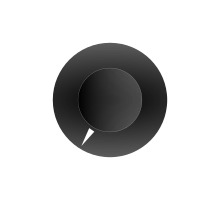
\includegraphics{images/volume_lo.png}
    & 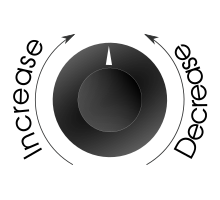
\includegraphics{images/volume.png}
    & 
\includegraphics{images/volume_hi.png}
\end{tabular}
\caption{Volume Control}
\end{table}

%%%%%%%%%%%%%%%%%%%%%%%%%%%%%%%%%%%%%%%%%%%%%%%%%%%%%%%%%%%%%%%%%%%%%%%%%%%%%%%%
% Symbols
%%%%%%%%%%%%%%%%%%%%%%%%%%%%%%%%%%%%%%%%%%%%%%%%%%%%%%%%%%%%%%%%%%%%%%%%%%%%%%%%
\section{Symbols}  \label{Audio - Symbols}

There are a number of symbols that will be used in the next sections to
describe the controls and actions that can be performed.

\ers{2.8}
\begin{longtabu}{ X[1,c,m] | X[4,l,m] }
  \thrule
  \multicolumn{2}{c}{\thb{Controls}} \\ \mrule
  \thbi{Symbol} & \thbi{Meaning} \\ \mrule

  \sPl & \cPl{f} push-button. \\ \drule{2}
  \sNe & \cNe{f} push-button. \\ \drule{2}
  \sPr & \cPr{f} push-button. \\ \thrule

  \multicolumn{2}{c}{\thb{Actions}} \\ \mrule
  \thbi{Symbol} & \thbi{Meaning} \\ \mrule

  \sPlay
    & Press \& Release \thinspace\sPl\enspace to \sAuPl{f} the \mAu{f}
      when it is in the \sAuPa{f} or \sAuSt{f} states. \\ \drule{2}
  \sPause
    & Press \& Release \thinspace\sPl\enspace to \sAuPa{f} the \mAu{f}
      when it is in the \sAuPl{f} state. \\ \drule{2}
  \sStop
    & Press \& Hold \thinspace\sPl\enspace until \symD{StOP}
      is displayed then release to \sAuSt{f} the \mAu{f}
      when it is in the \sAuPl{f} or \sAuPa{f} states. \\ \drule{2}
  \sNext
    & Press \& Release or Press \& Hold \thinspace\sNe\enspace to \sAuSk{f}
      forward tracks. \\ \drule{2}

  \pagebreak \drule{2}
  \sPrev
    & Press \& Release or Press \& Hold \thinspace\sPr\enspace to \dRe{f}
      the current track or \sAuSk{f} backward tracks. \\

  \bhrule
\caption{Audio - Symbols}
\end{longtabu}

%%%%%%%%%%%%%%%%%%%%%%%%%%%%%%%%%%%%%%%%%%%%%%%%%%%%%%%%%%%%%%%%%%%%%%%%%%%%%%%%
% Play|Pause|Stop
%%%%%%%%%%%%%%%%%%%%%%%%%%%%%%%%%%%%%%%%%%%%%%%%%%%%%%%%%%%%%%%%%%%%%%%%%%%%%%%%
\section{Play | Pause | Stop} \label{Audio - Play|Pause|Stop}

The \thinspace\sPl\enspace push-button can \sAuPl{f}, \sAuPa{f} or \sAuSt{f}
the \mAu{f}.

\par\medskip

The \mAu{f} starts in the \sAuSt{f} state when the device is initially switched
\sOn{f} via the \cPo{f}.  To start playback, \aPR{f}.

\ase{1}{{c c c c}}{%
\sAuSt{sym} & \sPlay & \eStart{sym}{PLAYBACK} & \sAuPl{sym} \\}

To \sAuPa{f}, \aPR{f} when in the \sAuPl{f} state.

\ase{1}{{c c c c}}{%
\sAuPl{sym} & \sPause & \ePa{sym}{PLAYBACK} & \sAuPa{sym} \\}

To resume playback, \aPR{f} when in the \sAuPa{f} state.

\ase{1}{{c c c c}}{%
\sAuPa{sym} & \sPlay & \eResume{sym}{PLAYBACK} & \sAuPl{sym} \\}

To \sAuSt{f} the \mAu{f} when in \sAuPl{f} or \sAuPa{f} states, \aPH{f} for
\mono{2} seconds and \aRe{f} when the \cDi{f} shows

\begin{figure}[H]
\centering
  \sDl{StOP}
\end{figure}

\ase{1}{{c c c c}}{%
\sAuPl{sym} & \multirow{2}{*}{\sStop} & \multirow{2}{*}{\eSt{sym}{PLAYBACK}}
  & \multirow{2}{*}{\sAuSt{sym}} \\ \dcrule{1}{1}
\sAuPa{sym} & & & \\}

Besides the power savings that \sAuSt{f} provides over \sAuPa{f},
there is another difference between \sAuPa{f} and \sAuSt{f}.

\begin{itemize}
  \item When resuming from \sAuPa{f}, the the track will resume playing from
    the same place as when it was paused.
  \item When resuming from \sAuSt{f}, the track will start playing from the
    beginning.
\end{itemize}

%%%%%%%%%%%%%%%%%%%%%%%%%%%%%%%%%%%%%%%%%%%%%%%%%%%%%%%%%%%%%%%%%%%%%%%%%%%%%%%%
% Next
%%%%%%%%%%%%%%%%%%%%%%%%%%%%%%%%%%%%%%%%%%%%%%%%%%%%%%%%%%%%%%%%%%%%%%%%%%%%%%%%
\section{Next} \label{Audio - Next}

The \thinspace\sNe\enspace push-button is used to \aSkip{f} \textit{forward}
one or more tracks.  

\begin{itemize}
  \item \aPR{f} to \aSkip{f} to the \textit{next} track.
    \begin{itemize}
      \item The next track number will \textit{not} be shown on the \cDi{f}.
    \end{itemize}
  \item \aPH{f} to \aSkip{f} \textit{forward} one or more tracks.
    \begin{itemize}
      \item The longer the push-button is held, the faster tracks will progress.
      \item The track numbers \textit{will} be shown on the \cDi{f}, for
        example:
        \figD{!!22}{Track \#22}
      \item \aRe{f} when you get to the track you want.
    \end{itemize}
\end{itemize}

\as{{c c c c c}}{%
\sAuPl{sym} & & & & \\ \dcrule{1}{1}
\sAuPa{sym} & \sNext & \sAuSk{sym} & \eSk{sym}{FORWARD} & \sAuPl{sym} \\ \dcrule{1}{1}
\sAuSt{sym} & & & & \\}

\begin{table}[H]
\ers{1}
\centering
\begin{tabu} { X[1,c,m] | X[1,c,m] }
  \thrule
  \thbi{Hold Time} & \thbi{Tracks per Second} \\ \mrule
  First \num{5} Tracks & \num{1} \\ \drule{2}
  Next \num{10} Tracks & \num{2} \\ \drule{2}
  Next \num{20} Tracks & \num{4} \\ \drule{2}
  Next \num{40} Tracks & \num{8} \\ \drule{2}
  Next \num{80} Tracks & \num{16} \\ \drule{2}
  Next \textit{\large\mono{N}} Tracks & \num{32} \\
  \bhrule
\end{tabu}
\caption{Audio - Next Hold Times}
\end{table}

\info{When the device is in the \sPoSl{f} power state, \sNe\enspace
can \textit{not} wake it - see \hyperref[Power]{\mPo{f}} for more
information and controls that can wake the device from \sPoSl{f}.}

%%%%%%%%%%%%%%%%%%%%%%%%%%%%%%%%%%%%%%%%%%%%%%%%%%%%%%%%%%%%%%%%%%%%%%%%%%%%%%%%
% Previous
%%%%%%%%%%%%%%%%%%%%%%%%%%%%%%%%%%%%%%%%%%%%%%%%%%%%%%%%%%%%%%%%%%%%%%%%%%%%%%%%
\section{Previous} \label{Audio - Previous}

The \thinspace\sPr\enspace push-button is used to \aSkip{f} \textit{backward}
one or more tracks or \dRe{f} the current track.

\begin{itemize}
  \item \aPR{f}
    \begin{itemize}
      \item \dRe{f} the current track if more than $\frac{1}{4}$ of the track
        has played.
      \item Otherwise, \aSkip{f} to the \textit{previous} track.
      \item The track number will \textit{not} be shown on the \cDi{f}.
    \end{itemize}
  \item \aPH{f} to \aSkip{f} \textit{backward} one or more tracks.
    \begin{itemize}
      \item The longer the push-button is held, the faster tracks will progress.
      \item The track numbers \textit{will} be shown on the \cDi{f}, for example:
        \figD{!!!8}{Track \#8}
      \item \aRe{f} when you get to the track you want.
    \end{itemize}
\end{itemize}

\as{{c c c c c}}{%
\sAuPl{sym} & \multirow{3}{*}[-1.5mm]{\sPrev} & \multirow{3}{*}[-1.5mm]{\sAuSk{sym}}
  & \multirow{3}{*}[-2.5mm]{%
    \begin{tabu}{c} \eRewind{sym}{CURRENT TRACK} \\ \drule{1} \eSk{sym}{BACKWARD} \end{tabu}}
  & \multirow{3}{*}{\sAuPl{sym}} \\ \dcrule{1}{1}
\sAuPa{sym} & & & & \\ \dcrule{1}{1}
\sAuSt{sym} & & & & \\}

\begin{table}[H]
\ers{1}
\centering
\begin{tabu}{ X[1,c,m] | X[1,c,m] }
  \thrule
  \thbi{Hold Time} & \thbi{Tracks per Second} \\ \mrule
  First \num{5} Tracks & \num{1} \\ \drule{2}
  Next \num{10} Tracks & \num{2} \\ \drule{2}
  Next \num{20} Tracks & \num{4} \\ \drule{2}
  Next \num{40} Tracks & \num{8} \\ \drule{2}
  Next \num{80} Tracks & \num{16} \\ \drule{2}
  Next \textit{\large\mono{N}} Tracks & \num{32} \\
  \bhrule
\end{tabu}
\caption{Audio - Previous Hold Times}
\end{table}

\info{When the device is in the \sPoSl{f} power state, \sPr\enspace
can \textit{not} wake it - see \hyperref[Power]{\mPo{f}} for more
information and controls that can wake the device from \sPoSl{f}.}

%%%%%%%%%%%%%%%%%%%%%%%%%%%%%%%%%%%%%%%%%%%%%%%%%%%%%%%%%%%%%%%%%%%%%%%%%%%%%%%%
% Track Selection
%%%%%%%%%%%%%%%%%%%%%%%%%%%%%%%%%%%%%%%%%%%%%%%%%%%%%%%%%%%%%%%%%%%%%%%%%%%%%%%%
\section{Track Selection} \label{Audio - Track Selection}

In addition to using the \cNe{f} and \cPr{f} controls to \sAuSk{f} forward and
backward in order to select a track for playback, there also exists the
capability to select a track more quickly and directly when in
\hyperref[Clock]{\mCl{f}} mode.  The \cEs{f} can be used alone or in
combination with \aTo{f} to do so.  Refer to \hyperref[Show Track]{Show Track}
and \hyperref[Set Track]{Set Track} in that section for more information.

%%%%%%%%%%%%%%%%%%%%%%%%%%%%%%%%%%%%%%%%%%%%%%%%%%%%%%%%%%%%%%%%%%%%%%%%%%%%%%%%
% Reference
%%%%%%%%%%%%%%%%%%%%%%%%%%%%%%%%%%%%%%%%%%%%%%%%%%%%%%%%%%%%%%%%%%%%%%%%%%%%%%%%
\section{Reference} \label{Audio - Reference}

\ers{2}
\begin{longtabu}{ X[2,c,m] | X[2,c,m] | X[2,c,m] | X[4,c,m] | X[2,c,m] }
  \thrule

  \thbi{State} & \thbi{Action} & \thbi{Control} & \thbi{Effect} & \thbi{Next} \\ \mdrule

  \multirow{3}{*}[-1.5mm]{\sAuSt{sym}}
    & \sPlay & \sPl & \ePl{sym}{AUDIO} & \sAuPl{sym} \\ \dcrule{2}{5}
  & \sNext & \sNe & \eSk{sym}{FORWARD}
    & \multirow{2}{*}[-1mm]{\sAuSk{sym}} \\ \dcrule{2}{4}
  & \sPrev & \sPr & \eSk{sym}{BACKWARD} & \\ \mrule

  \multirow{4}{*}[-1.5mm]{\sAuPl{sym}}
    & \sPause & \sPl & \ePa{sym}{AUDIO} & \sAuPa{sym} \\ \dcrule{2}{5}
  & \sNext & \sNe & \eSk{sym}{FORWARD}
    & \multirow{2}{*}[-1mm]{\sAuSk{sym}} \\ \dcrule{2}{4}
  & \sPrev & \sPr & \eSk{sym}{BACKWARD} & \\ \dcrule{2}{5}
  & \sStop & \sPl & \eSt{sym}{AUDIO} & \sAuSt{sym} \\ \mrule

  \multirow{5}{*}[-1.5mm]{\sAuPa{sym}}
    & \sPlay & \sPl & \eResume{sym}{AUDIO} & \sAuPl{sym} \\ \dcrule{2}{5}
  & \sNext & \sNe & \eSk{sym}{FORWARD}
    & \multirow{2}{*}[-1mm]{\sAuSk{sym}} \\ \dcrule{2}{4}
  & \sPrev & \sPr & \eSk{sym}{BACKWARD} & \\ \dcrule{2}{5}
  & \sStop & \sPl & \multirow{2}{*}[-1mm]{\eSt{sym}{AUDIO}}
    & \multirow{2}{*}[-1mm]{\sAuSt{sym}} \\ \dcrule{2}{3}
  & \action{ss}{INACTIVITY} & --- & & \\ \mrule

  \pagebreak
  \mrule

  \multirow{4}{*}[-1mm]{\sAuSk{sym}} & \sNext & \sNe
    & \eSk{sym}{FORWARD} & \multirow{2}{*}[-1mm]{---} \\ \dcrule{2}{4}
  & \sPrev & \sPr & \eSk{sym}{BACKWARD} & \\ \dcrule{2}{5}
  & \multirow{2}{*}[-1mm]{\action{ss}{RELEASE}} & \sNe
    & \multirow{2}{*}[-1mm]{\ePl{sym}{TRACK}}
    & \multirow{2}{*}[-1mm]{\sAuPl{sym}} \\ \dcrule{3}{3}
  & & \sPr & & \\

  \bhrule
\caption {Audio - Reference}
\end{longtabu}

%%%%%%%%%%%%%%%%%%%%%%%%%%%%%%%%%%%%%%%%%%%%%%%%%%%%%%%%%%%%%%%%%%%%%%%%%%%%%%%%
% Audio - State Diagram
%%%%%%%%%%%%%%%%%%%%%%%%%%%%%%%%%%%%%%%%%%%%%%%%%%%%%%%%%%%%%%%%%%%%%%%%%%%%%%%%
\section{State Diagram} \label{Audio - State Diagram}

\begin{figure}[H]
  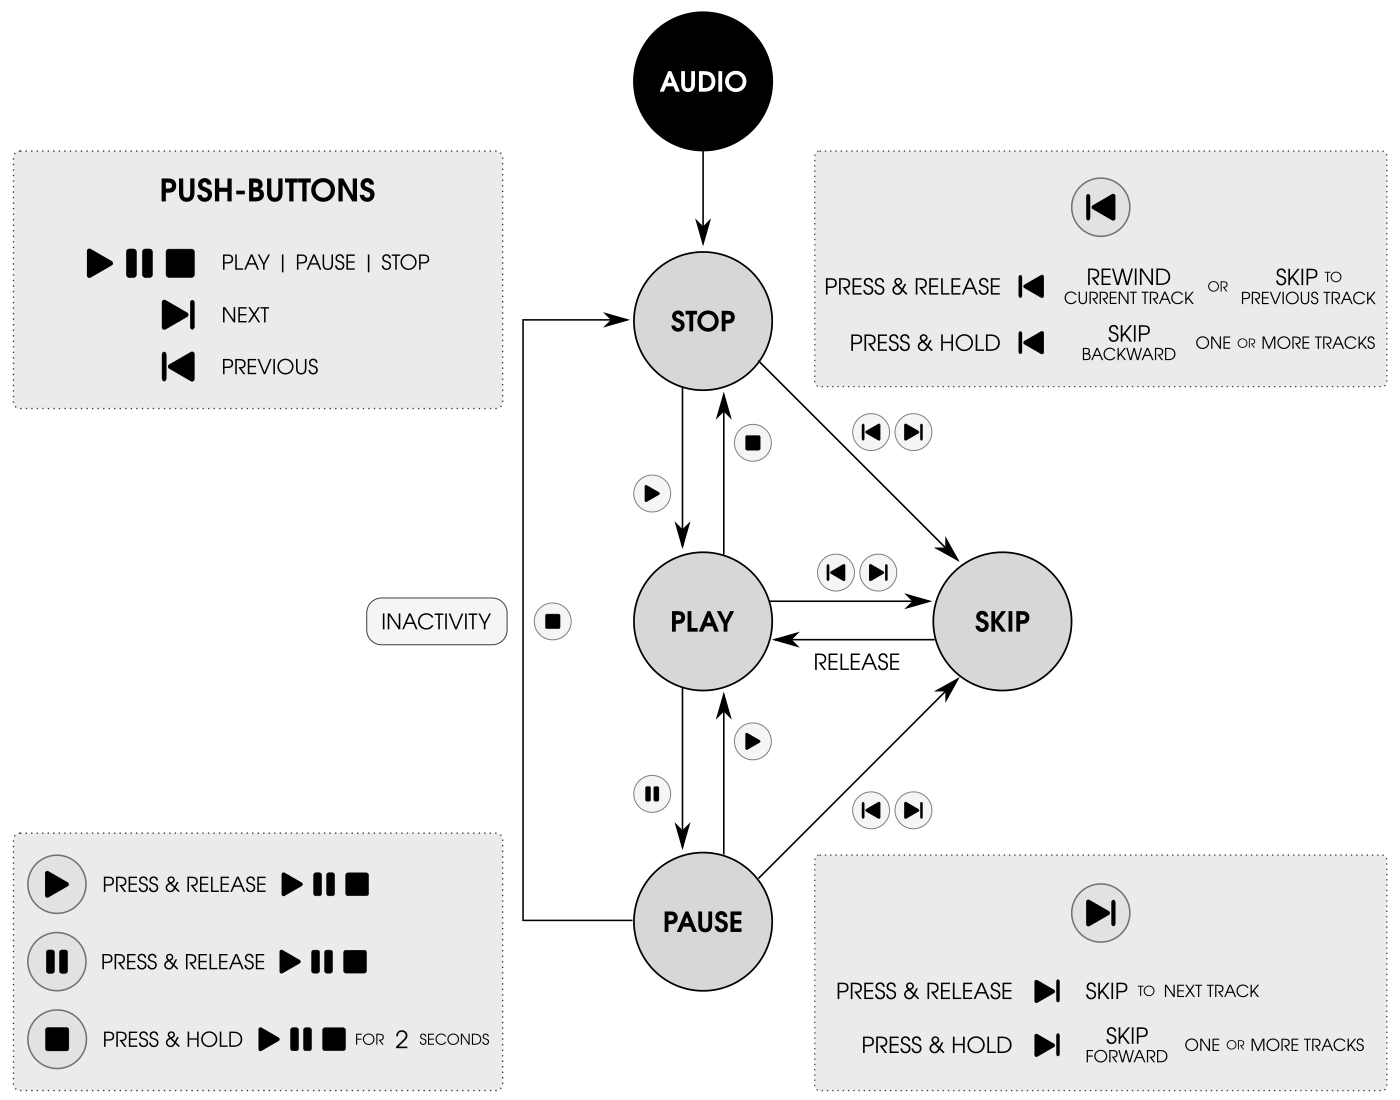
\includegraphics{images/audio_state_diagram.png}
\caption{Audio - State Diagram}
\end{figure}

%%%%%%%%%%%%%%%%%%%%%%%%%%%%%%%%%%%%%%%%%%%%%%%%%%%%%%%%%%%%%%%%%%%%%%%%%%%%%%%%
% Alarm
%%%%%%%%%%%%%%%%%%%%%%%%%%%%%%%%%%%%%%%%%%%%%%%%%%%%%%%%%%%%%%%%%%%%%%%%%%%%%%%%
\chapter{Alarm} \label{Alarm}
\vspace{-10ex}\mAl{syml}\vskip 8ex

%%%%%%%%%%%%%%%%%%%%%%%%%%%%%%%%%%%%%%%%%%%%%%%%%%%%%%%%%%%%%%%%%%%%%%%%%%%%%%%%
% Introduction
%%%%%%%%%%%%%%%%%%%%%%%%%%%%%%%%%%%%%%%%%%%%%%%%%%%%%%%%%%%%%%%%%%%%%%%%%%%%%%%%
\section{Introduction}

The \mAl{f} is a \textit{time of day} alarm.  It runs independent of any mode
and can wake the device from any power state.  Both the \cBe{f} and \mAu{f}
can be used as wakeup sources.  Refer to \hyperref[Set Alarm]{\mSA{f}}
for configuration.

%%%%%%%%%%%%%%%%%%%%%%%%%%%%%%%%%%%%%%%%%%%%%%%%%%%%%%%%%%%%%%%%%%%%%%%%%%%%%%%%
% Disabled
%%%%%%%%%%%%%%%%%%%%%%%%%%%%%%%%%%%%%%%%%%%%%%%%%%%%%%%%%%%%%%%%%%%%%%%%%%%%%%%%
\section{Disabled} \label{Alarm - Disabled} \sAlDi{syml}

If the alarm is \sAlDi{f}, it will stay in the \sAlDi{f} state until enabled
via \hyperref[Set Alarm]{\mSA{f}}.

%%%%%%%%%%%%%%%%%%%%%%%%%%%%%%%%%%%%%%%%%%%%%%%%%%%%%%%%%%%%%%%%%%%%%%%%%%%%%%%%
% Off
%%%%%%%%%%%%%%%%%%%%%%%%%%%%%%%%%%%%%%%%%%%%%%%%%%%%%%%%%%%%%%%%%%%%%%%%%%%%%%%%
\section{Off} \label{Alarm - Off} \sAlOf{syml}

This is the initial and final state if the alarm is enabled.  When the current
time equals the alarm time, the alarm will start, and either

\begin{enumerate}
  \item Start playing an \mAu{f} track, or
  \item Start alerting with the \cBe{f}
\end{enumerate}

depending on which was configured in \mSA{f}. It will then enter the \sAlWa{f}
state.

\as{{c c c c}}{\sAlOf{sym} & \aTi{sym} & \eStart{sym}{ALARM} & \sAlWa{sym} \\}

\info{If a track is currently playing when the alarm starts, the beeper will be
used regardless of setting - this is so you know that the alarm has started.}

%%%%%%%%%%%%%%%%%%%%%%%%%%%%%%%%%%%%%%%%%%%%%%%%%%%%%%%%%%%%%%%%%%%%%%%%%%%%%%%%
% Wake
%%%%%%%%%%%%%%%%%%%%%%%%%%%%%%%%%%%%%%%%%%%%%%%%%%%%%%%%%%%%%%%%%%%%%%%%%%%%%%%%
\section{Wake} \label{Alarm - Wake} \sAlWa{syml}

In this state, the \cBe{f} will alert or the \mAu{f} will play a track.  To
\sAlSn{f} the alarm, do one of the following:

\begin{itemize}
  \item \aTo{f} the \dTo{f} of the enclosure.\footnote{ This assumes that touch
    has been enabled via \hyperref[Touch Settings]{\mTS{ss}}.}
  \item \aTu{f} the \cEs{f}.
\end{itemize}

\as{{c c c c}}{%
\multirow{2}{*}{\sAlWa{sym}} & \sTo
  & \multirow{2}{*}{\eSnooze{sym}{ALARM}}
  & \multirow{2}{*}{\sAlSn{sym}} \\ \dcrule{2}{2}
& \sTu & & \\}

The \cDi{f} will show

\begin{figure}[H]
\centering
  \sDl{Snoo}
\end{figure}

when either of the two above actions are taken.

\par\medskip

If a \sSAWT{f} has been configured and the alarm has been in the \sAlWa{f}
state for longer than that time, the alarm will stop and go to the \sAlOf{f}
state.

\as{{c c c}}{\sAlWa{sym} & \aWT{sym} & \sAlOf{sym} \\}

%%%%%%%%%%%%%%%%%%%%%%%%%%%%%%%%%%%%%%%%%%%%%%%%%%%%%%%%%%%%%%%%%%%%%%%%%%%%%%%%
% Snooze
%%%%%%%%%%%%%%%%%%%%%%%%%%%%%%%%%%%%%%%%%%%%%%%%%%%%%%%%%%%%%%%%%%%%%%%%%%%%%%%%
\section{Snooze} \label{Alarm - Snooze} \sAlSn{syml}

The \mAu{f} will be paused or the \cBe{f} will stop when the alarm is snoozed.
It will resume when the configured \sSAST{f} has elapsed.

\as{{c c c c}}{\sAlSn{sym} & \aST{sym} & \eResume{sym}{ALARM} & \sAlWa{sym} \\}

%%%%%%%%%%%%%%%%%%%%%%%%%%%%%%%%%%%%%%%%%%%%%%%%%%%%%%%%%%%%%%%%%%%%%%%%%%%%%%%%
% In Progress
%%%%%%%%%%%%%%%%%%%%%%%%%%%%%%%%%%%%%%%%%%%%%%%%%%%%%%%%%%%%%%%%%%%%%%%%%%%%%%%%
\section{In Progress} \label{Alarm - In Progress} \sAlIP{syml}

This includes both the \sAlWa{f} and \sAlSn{f} states.  To stop the alarm,
\aPR{f} the \cEs{f}.

\par\medskip

The \cDi{f} will show

\begin{figure}[H]
\centering
  \sDl{OFF!}
\end{figure}

when the above action is taken.

\as{{c c c c}}{\sAlIP{sym} & \sPR & \eSt{sym}{ALARM} & \sAlOf{sym} \\}

If a \sSATT{f} has been configured and the alarm has been \sAlIP{f} for
more than this time, it will turn off and go to the \sAlOf{f} state.

\as{{c c c}}{\sAlIP{sym} & \aTT{sym} & \sAlOf{sym} \\}

In either case, the alarm will automatically reset for the next day.

%%%%%%%%%%%%%%%%%%%%%%%%%%%%%%%%%%%%%%%%%%%%%%%%%%%%%%%%%%%%%%%%%%%%%%%%%%%%%%%%
% Reference
%%%%%%%%%%%%%%%%%%%%%%%%%%%%%%%%%%%%%%%%%%%%%%%%%%%%%%%%%%%%%%%%%%%%%%%%%%%%%%%%
\section{Reference} \label{Alarm - Reference}

\ers{2}
\begin{longtabu}{ X[2,c,m] | X[2,c,m] | X[3,c,m] | X[2,c,m] }
  \thrule
  \thbi{State} & \thbi{Action} & \thbi{Effect} & \thbi{Next} \\ \mdrule

  \sAlDi{sym} & --- & --- & --- \\ \mrule

  \sAlOf{sym} & \fontTGA{ss}{TIME = ALARM TIME}
    & \eStart{sym}{ALARM} & \sAlWa{sym} \\ \mrule

  \multirow{5}{*}[-1.5mm]{\sAlWa{sym}}
    & \sTo & \multirow{2}{*}[-1mm]{\eSnooze{sym}{ALARM}}
    & \multirow{2}{*}[-1mm]{\sAlSn{sym}} \\ \dcrule{2}{2}
  & \sTu & & \\ \dcrule{2}{4}
  & \sPR & & \\ \dcrule{2}{2}
  & \fontTGA{ss}{WAKE TIME EXCEEDED}
    & \eSt{sym}{ALARM} & \sAlOf{sym} \\ \dcrule{2}{2}
  & \fontTGA{ss}{TOTAL ALARM TIME EXCEEDED} & & \\ \mrule

  & \fontTGA{ss}{SNOOZE TIME EXPIRED}
    & \eWake{sym}{ALARM} & \sAlWa{sym} \\ \dcrule{2}{4}

  \sAlSn{sym} & \sPR
    & \multirow{2}{*}[-1mm]{\eSt{sym}{ALARM}}
    & \multirow{2}{*}[-1mm]{\sAlOf{sym}} \\ \dcrule{2}{2}

  & \fontTGA{ss}{TOTAL ALARM TIME EXCEEDED} & & \\

  \bhrule
\caption{Alarm - Reference}
\end{longtabu}

%%%%%%%%%%%%%%%%%%%%%%%%%%%%%%%%%%%%%%%%%%%%%%%%%%%%%%%%%%%%%%%%%%%%%%%%%%%%%%%%
% State Diagram
%%%%%%%%%%%%%%%%%%%%%%%%%%%%%%%%%%%%%%%%%%%%%%%%%%%%%%%%%%%%%%%%%%%%%%%%%%%%%%%%
\section{State Diagram} \label{Alarm - State Diagram}

\begin{figure}[H]
\centering
  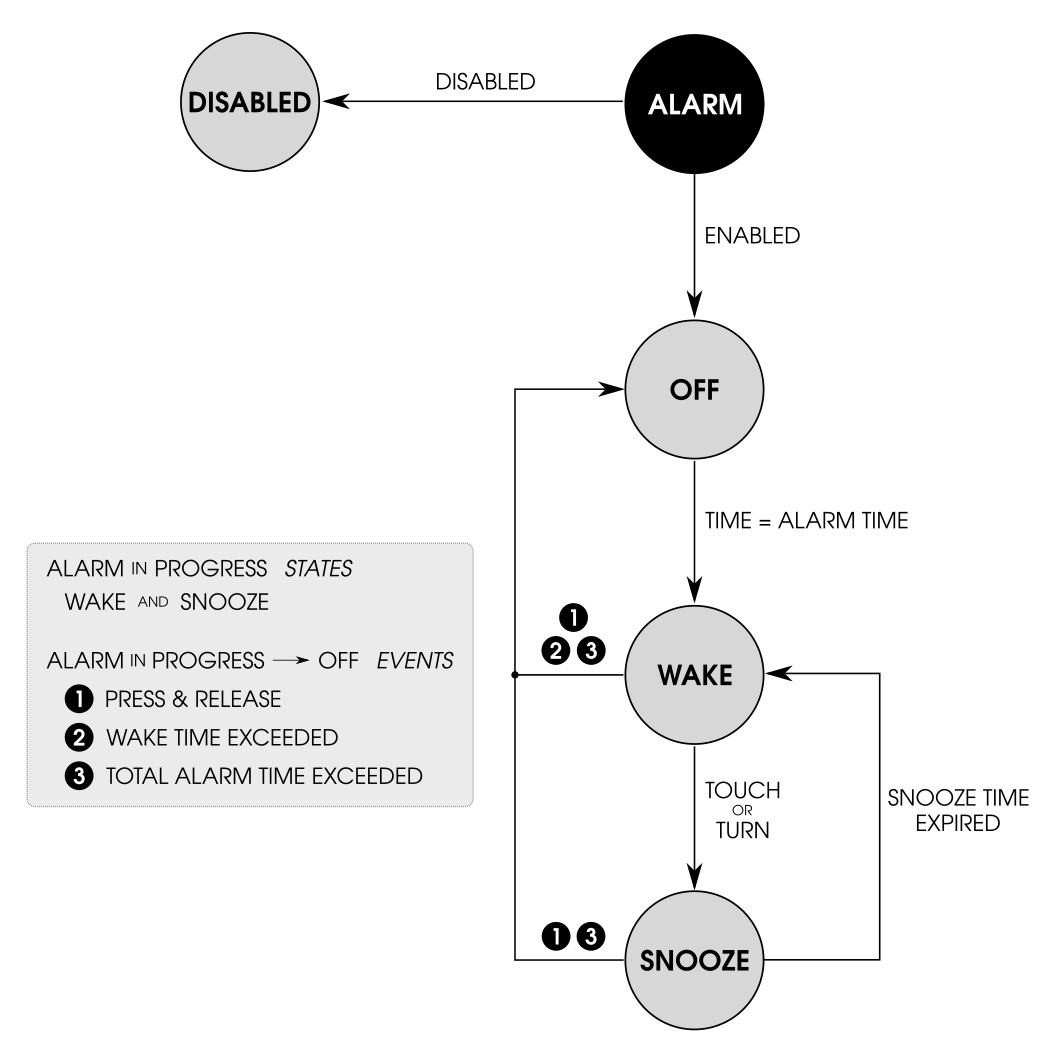
\includegraphics{images/alarm_state_diagram.png}
\caption{Alarm - State Diagram}
\end{figure}

%%%%%%%%%%%%%%%%%%%%%%%%%%%%%%%%%%%%%%%%%%%%%%%%%%%%%%%%%%%%%%%%%%%%%%%%%%%%%%%%
% Power
%%%%%%%%%%%%%%%%%%%%%%%%%%%%%%%%%%%%%%%%%%%%%%%%%%%%%%%%%%%%%%%%%%%%%%%%%%%%%%%%
\chapter{Power} \label{Power}
\vspace{-10ex}\mPo{syml}\vskip 8ex

%%%%%%%%%%%%%%%%%%%%%%%%%%%%%%%%%%%%%%%%%%%%%%%%%%%%%%%%%%%%%%%%%%%%%%%%%%%%%%%%
% Introduction
%%%%%%%%%%%%%%%%%%%%%%%%%%%%%%%%%%%%%%%%%%%%%%%%%%%%%%%%%%%%%%%%%%%%%%%%%%%%%%%%
\section{Introduction}

In order to prolong battery charge, the \cDi{f} and \cLi{f} can, depending on
mode, turn \sScOf{f} or \sScDi{f} after a configurable period of inactivity.
The device can also enter a low power \sPoSl{f} state to further reduce power
consumption and auto-stop the \mAu{f} if it isn't being used.  See
\hyperref[Power Settings]{\mPS{f}} for configuration.

%%%%%%%%%%%%%%%%%%%%%%%%%%%%%%%%%%%%%%%%%%%%%%%%%%%%%%%%%%%%%%%%%%%%%%%%%%%%%%%%
% Wake
%%%%%%%%%%%%%%%%%%%%%%%%%%%%%%%%%%%%%%%%%%%%%%%%%%%%%%%%%%%%%%%%%%%%%%%%%%%%%%%%
\section{Wake} \label{Power - Wake} \sPoAw{syml}

This is the normal operating state and also is the most power consumptive.
The \cDi{f} is \sScOn{f} and the \cLi{f} window is potentially lit, both at the
brightness level as determined by the \cBr{f}.

\par\medskip

Any kind of interaction with the controls of the device will either wake it or
keep it awake.

\begin{itemize}
  \item \aTo{f} the \dTo{f} of the device.\footnote{ Assumes touch capability
    has been enabled via \hyperref[Touch Settings]{\mTS{ss}}.}.
  \item \aTu{f} the \cRs{f}.
  \item \aTu{f} or \aPr{f} the \cEs{f}.
  \item \aTu{f} the \cBr{f}.
  \item \aPr{f} the \cPl{f}, \cNe{f} or \cPr{f} push-buttons.
\end{itemize}

\info{If in the \sPoSl{f} state, neither the \cNe{f} nor the \cPr{f}
push-buttons can wake it though they will keep it from going into a \sPoSl{f}
state.}

\par\medskip

\info{When in \mTS{f} mode and the power state is \sPoNa{f}, \aTo{f} will not
wake it.}

\ers{1}
\begin{longtabu} { X[1,c,m] | X[2,c,m] }
  \thrule
  \thbi{Action} & \thbi{Control} \\ \mrule

  \multirow{3}{*}{\aTu{n}}
    & \hyperref[Operation - Selector Dial]{\cRs{f}} \\
    & \hyperref[Operation - Settings Knob]{\cEs{f}} \\
    & \hyperref[Brightness Knob]{\cBr{f}} \\ \drule{2}

  \multirow{4}{*}{\aPr{n}}
    & \hyperref[Operation - Settings Knob]{\cEs{f}} \\
    & \hyperref[Audio - Play|Pause|Stop]{\cPl{f}} \\
    & \hyperref[Audio - Next]{\cNe{f}}\footnote{ The \cNe{ss} push-button
      will \textit{not} wake if sleeping.} \\
    & \hyperref[Audio - Previous]{\cPr{f}}\footnote{ The \cPr{ss} push-button
      will \textit{not} wake if sleeping.} \\ \drule{2}

  \aTo{n} & \hyperref[Operation - Touch Sensor]{\cTS{f}}\footnote{ Touch
    will \textit{not} wake when napping and in \mTS{ss} mode.} \\

  \bhrule
\caption{Power - Waking Control Actions}
\end{longtabu}

Additionally, the \mAl{f} will wake the device from any power state. It will
also keep it from entering a \sPoSl{f} state as long as it is in the \sAlWa{f}
state and actively alerting or playing music or \sAlIP{f} and the wakeup source
is the \mAu{f}.

%%%%%%%%%%%%%%%%%%%%%%%%%%%%%%%%%%%%%%%%%%%%%%%%%%%%%%%%%%%%%%%%%%%%%%%%%%%%%%%%
% Nap
%%%%%%%%%%%%%%%%%%%%%%%%%%%%%%%%%%%%%%%%%%%%%%%%%%%%%%%%%%%%%%%%%%%%%%%%%%%%%%%%
\section{Nap} \label{Power - Nap} \sPoNa{syml}

The device will \sPoNa{f} if a nap timer has been enabled via
\hyperref[Power Settings]{\mPS{f}} and the following conditions are met:

\begin{itemize}
  \item You are \textit{not} actively using the device, i.e. not interacting
    with it or fiddling with the controls.
  \item The nap timer is enabled and the configured nap timer has elapsed.
\end{itemize}

The nap timer is started from the last time the device was interacted with. For
example, if the \cEs{f} was just turned, the timer will start from that point.
As long as you are interacting with the device, it will \textit{not} \sPoNa{f}.

\par\medskip

The screens will either \sDim{f} or turn \sOff{f} depending on the current mode
and state.

\begin{table}[H]
  \begin{tabu} { X[1,c,m] | X[1,c,m] | X[1,c,m] }
  \thrule
  \thbi{Mode} & \thbi{State} & \thbi{Screens} \\ \mrule

  \hyperref[Clock]{\mCl{s}} & \state{f}{ANY} & \sDim{sym} \\ \mrule

  \multirow{3}{*}[-2.0mm]{\hyperref[Timer]{\mTi{s}}}
    & \sTiRu{f} & \multirow{2}{*}{\sDim{sym}} \\
    & \sTiAl{f} & \\ \dcrule{2}{3}
    & \fontTGA{ss}{ALL OTHER STATES} & \sOff{sym} \\ \mrule

  \multirow{5}{*}[-2.0mm]{\hyperref[Touch Settings]{\mTS{s}}}
    & \sTSBR{f} & \multirow{4}{*}{\sDim{sym}} \\
    & \sTSTR{f} & \\
    & \sTSRT{f} & \\
    & \sTSTA{f} & \\ \dcrule{2}{3}
    & \fontTGA{ss}{ALL OTHER STATES} & \sOff{sym} \\ \mrule

  \fontTGA{f}{ALL OTHER MODES} & \state{f}{ANY} & \sOff{sym} \\

  \bhrule
  \end{tabu}
\caption{Power - Nap Action per Mode}
\end{table}

%%%%%%%%%%%%%%%%%%%%%%%%%%%%%%%%%%%%%%%%%%%%%%%%%%%%%%%%%%%%%%%%%%%%%%%%%%%%%%%%
% Sleep
%%%%%%%%%%%%%%%%%%%%%%%%%%%%%%%%%%%%%%%%%%%%%%%%%%%%%%%%%%%%%%%%%%%%%%%%%%%%%%%%
\section{Sleep} \label{Power - Sleep} \sPoSl{syml}

When the device sleeps, the screens will turn \sOff{f}, the \mAu{f} will go into
the \sAuSt{f} state and all processing stops affording more power savings over
\sPoNa{f}.

\par\medskip

The device will \sPoSl{f} if a sleep timer has been enabled via
\hyperref[Power Settings]{\mPS{f}} and \textit{all} of the following conditions
are met:

\begin{itemize}
  \item You are not actively using the device, i.e. not interacting with it or
    fiddling with the controls.
  \item The \mAu{f} is \textit{not} in the \sAuPl{f} state.
  \item The \mAl{f} is \textit{not} in the \sAlWa{f} state.
  \item The \mAl{f} is \textit{not} \sAlIP{f} when the wakeup source is \mAu{f}.
  \item The current state in the current mode allows \sPoSl{f}.
  \item The sleep timer is enabled and the configured sleep timer has elapsed.
\end{itemize}

The sleep timer is started from the last time the device was interacted with.
For example, if the \cNe{f} push-button is being pressed, the timer will start
from that point.  As long as you are interacting with the device, it will
\textit{not} \sPoSl{f}.

\par\medskip

The timer is also restarted if the \mAu{f} is playing or the \mAl{f} is
alerting.  As long as the \mAu{f} is in the \sAuPl{f} state or the \mAl{f} is in
the \sAlWa{f} state, the device will \textit{not} \sPoSl{f}.

\par\medskip

Additionally, if the \mAl{f} is \sAlIP{f}, i.e. in the \sAlWa{f} or \sAlSn{f}
states \textit{and} the wakeup source is the \mAu{f}, the device will
\textit{not} \sPoSl{f}.  When the wakeup source is the \mAu{f} and the \mAl{f}
is snoozed, the \mAu{f} is \textit{not} stopped, but paused.  Since the
\sPoSl{f} state will \sAuSt{f} the \mAu{f}, the device will \textit{not}
\sPoSl{f} in this situation.

\par\medskip

\info{Though the \cNe{f} and \cPr{f} push-buttons can keep the device from
entering a \sPoSl{f} state, they can \textit{not} wake the device from
\sPoSl{f}.}

\par\medskip

Some modes can be in states that do \textit{not} allow the device to enter a
\sPoSl{f} state.  The following table shows which modes and states can and
cannot enter a \sPoSl{f} state.

\begin{table}[H]
  \begin{tabu} { X[1,c,m] | X[1,c,m] | X[1,c,m] }
  \thrule
  \thbi{Mode} & \thbi{State} & \thbi{Can Sleep?} \\ \mrule

  \multirow{3}{*}[-2.0mm]{\hyperref[Timer]{\mTi{s}}}
    & \sTiRu{f} & \multirow{2}{*}{\fontTGA{f}{NO}} \\
    & \sTiAl{f} & \\ \dcrule{2}{3}
    & \fontTGA{ss}{ALL OTHER STATES} & \fontTGA{f}{YES} \\ \mrule

  \multirow{5}{*}[-2.0mm]{\hyperref[Touch Settings]{\mTS{s}}}
    & \sTSBR{f} & \multirow{4}{*}{\fontTGA{f}{NO}} \\
    & \sTSTR{f} & \\
    & \sTSRT{f} & \\
    & \sTSTA{f} & \\ \dcrule{2}{3}
    & \fontTGA{ss}{ALL OTHER STATES} & \fontTGA{f}{YES} \\ \mrule

  \fontTGA{f}{ALL OTHER MODES} & \state{f}{ANY} & \fontTGA{f}{YES} \\
  \bhrule
  \end{tabu}
\caption{Power - Sleep per Mode \& State}
\end{table}

\pagebreak

Any mode or state that can not \sPoSl{f} will instead \sPoNa{f} and \sDim{f}
the screens.

\begin{table}[H]
  \begin{tabu} { X[1,c,m] | X[1,c,m] | X[1,c,m] }
  \thrule
  \thbi{Mode} & \thbi{State} & \thbi{Action} \\ \mrule

  \multirow{2}{*}[-1.0mm]{\hyperref[Timer]{\mTi{s}}}
    & \sTiRu{f} & \multirow{6}{*}{\sPoSl{f} $\longrightarrow$ \sPoNa{f}} \\
    & \sTiAl{f} & \\ \dcrule{1}{2}

  \multirow{4}{*}[-1.5mm]{\hyperref[Touch Settings]{\mTS{s}}}
    & \sTSBR{f} & \\
    & \sTSTR{f} & \\
    & \sTSRT{f} & \\
    & \sTSTA{f} & \\

  \bhrule
  \end{tabu}
\caption{Power - Sleep to Nap}
\end{table}

%%%%%%%%%%%%%%%%%%%%%%%%%%%%%%%%%%%%%%%%%%%%%%%%%%%%%%%%%%%%%%%%%%%%%%%%%%%%%%%%
% Sleep - Touch Sleep
%%%%%%%%%%%%%%%%%%%%%%%%%%%%%%%%%%%%%%%%%%%%%%%%%%%%%%%%%%%%%%%%%%%%%%%%%%%%%%%%
\subsection{Touch Sleep} \label{Power - Touch}

The device can be \textit{forced} into a \sPoSl{f} state by
\textit{continuously} touching the \cTo{f} of the device for a configurable
amount of time set via \hyperref[Power Settings]{\mPS{f}}.  Though the sleep
timer is reset when touched, it is irrelevant if this touch time is exceeded.
Since the device is forced into a \sPoSl{f} state, the \mAu{f} will be
\textit{forced} into the \sAuSt{f} state.

\info{For touch induced sleep to work, \aTo{f} must be enabled via
\hyperref[Touch Settings]{\mTS{f}} and the palm of your hand or
most of your fingers must lay on \cTo{f} of the enclosure.}

%%%%%%%%%%%%%%%%%%%%%%%%%%%%%%%%%%%%%%%%%%%%%%%%%%%%%%%%%%%%%%%%%%%%%%%%%%%%%%%%
% Audio Auto-Stop
%%%%%%%%%%%%%%%%%%%%%%%%%%%%%%%%%%%%%%%%%%%%%%%%%%%%%%%%%%%%%%%%%%%%%%%%%%%%%%%%
\section{Audio Auto-Stop} \label{Power - Stop}

The \mAu{f} component will automatically \sAuSt{f} if a stop timer has been
enabled via \hyperref[Power Settings]{\mPS{f}} and \textit{all} of the
following conditions are met:

\begin{itemize}
  \item You are not actively using the device, i.e. not interacting with it or
    fiddling with the controls.
  \item The \mAu{f} is in the \sAuPa{f} state.
  \item The \mAl{f} is \textit{not} \sAlIP{f} \textit{or} is \textit{not} using
    the \mAu{f} as the wakeup source.
  \item The stop timer is enabled and the configured stop timer has elapsed.
\end{itemize}

The stop timer is started from the last time the device was interacted with.
For example, if the \cBr{f} was just turned, the timer will start from that
point.  As long as you are interacting with the device, the \mAu{f} will
\textit{not} be auto-stopped.

\par\medskip

The timer is also restarted if the \mAu{f} is playing or the \mAl{f} is
\sAlIP{f}, i.e. in the \sAlWa{f} or \sAlSn{f} states \textit{and}
the wakeup source is the \mAu{f}.  As long as these conditions are true,
the device will \textit{not} auto-stop the \mAu{f}.

%%%%%%%%%%%%%%%%%%%%%%%%%%%%%%%%%%%%%%%%%%%%%%%%%%%%%%%%%%%%%%%%%%%%%%%%%%%%%%%%
% State Diagram
%%%%%%%%%%%%%%%%%%%%%%%%%%%%%%%%%%%%%%%%%%%%%%%%%%%%%%%%%%%%%%%%%%%%%%%%%%%%%%%%
\section{State Diagram}

\begin{figure}[H]
\centering
  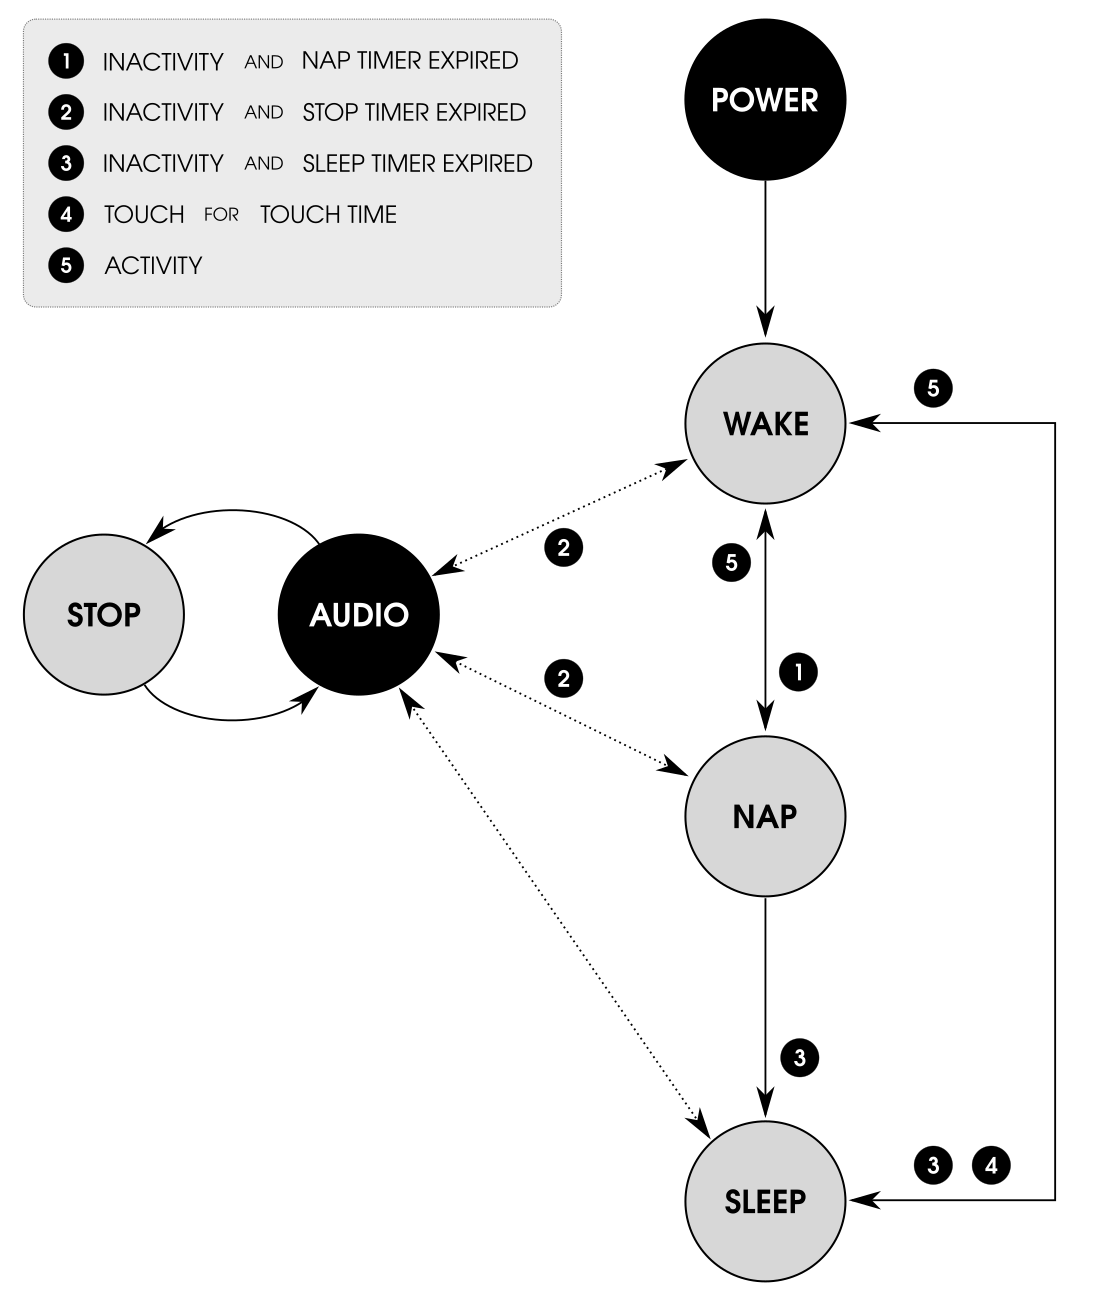
\includegraphics{images/power_state_diagram.png}
\caption{Power - State Diagram}
\end{figure}


%%%%%%%%%%%%%%%%%%%%%%%%%%%%%%%%%%%%%%%%%%%%%%%%%%%%%%%%%%%%%%%%%%%%%%%%%%%%%%%%
% Primary Modes
%%%%%%%%%%%%%%%%%%%%%%%%%%%%%%%%%%%%%%%%%%%%%%%%%%%%%%%%%%%%%%%%%%%%%%%%%%%%%%%%
\part{Primary Modes} \label{Primary Modes}
%%%%%%%%%%%%%%%%%%%%%%%%%%%%%%%%%%%%%%%%%%%%%%%%%%%%%%%%%%%%%%%%%%%%%%%%%%%%%%%%
% Clock
%%%%%%%%%%%%%%%%%%%%%%%%%%%%%%%%%%%%%%%%%%%%%%%%%%%%%%%%%%%%%%%%%%%%%%%%%%%%%%%%
\chapter{Clock} \label{Clock}
\vspace{-10ex}\mCl{syml}\vskip 8ex

%%%%%%%%%%%%%%%%%%%%%%%%%%%%%%%%%%%%%%%%%%%%%%%%%%%%%%%%%%%%%%%%%%%%%%%%%%%%%%%%
% Introduction
%%%%%%%%%%%%%%%%%%%%%%%%%%%%%%%%%%%%%%%%%%%%%%%%%%%%%%%%%%%%%%%%%%%%%%%%%%%%%%%%
\section{Introduction}

This is the mode the device will likely be in a majority of the time.  It
displays the current time and can display the date and current track number
and provides the capability to directly select a track for playback.  It is
also the only mode where you can turn the night light on and off.

\par\medskip

It is the \mPr{f} and \textit{only} mode when the \cRs{f} is in the \dMi{f}
position.

\par\medskip

To get to \mCl{f} mode simply \aTu{f} the \cRs{f} to the \dMi{f}.

\begin{table}[H]
\ers{3}
\centering
\begin{tabu} { X[1,c,m] | X[1,c,m] | X[1,c,m] }
  \thrule
  \thbi{Position} & \thbi{Mode} & \thbi{Action} \\ \mrule
  \sLe & \multirow{2}{*}[-1mm]{\mode{s}{ANY}}
    & $\hskip -4mm$ \sLtoM \\ \dcrule{1}{1} \dcrule{3}{3}
  \sRi & & $\hskip 4mm$ \sRtoM \\ \mdrule
  \sMi & \mCl{sym} & --- \\
  \bhrule
\end{tabu}
\caption{Clock - Mode}
\end{table}

%%%%%%%%%%%%%%%%%%%%%%%%%%%%%%%%%%%%%%%%%%%%%%%%%%%%%%%%%%%%%%%%%%%%%%%%%%%%%%%%
% Overview
%%%%%%%%%%%%%%%%%%%%%%%%%%%%%%%%%%%%%%%%%%%%%%%%%%%%%%%%%%%%%%%%%%%%%%%%%%%%%%%%
\pagebreak
\section{Overview}

There are a number of states the \mCl{f} can be in and are explained in the
following sections.

\begin{table}[H]
\ers{1}
\centering
\begin{tabu} { X[1,c,m] | X[3,l,m] }
  \thrule
  \thbi{State} & \thbi{Description} \\ \mrule
  \sClTi{sym} & Display the current time. \\ \drule{2}
  \sClMD{sym} & Display the month \& day. \\ \drule{2}
  \sClYe{sym} & Display the year.  \\ \drule{2}
  \sClSh{sym} & Display the current track number. \\ \drule{2}
  \sClSe{sym} & Select a track for playback. \\
  \bhrule
\end{tabu}
\caption{Clock - States}
\end{table}

To progress through the states, \aPR{f} the \cEs{f}.  The basic progression from
\sClTi{f} back to \sClTi{f} is:

\as{{ c c c c c c c c c }}{%
\sClTi{sym} & \sPR & \sClMD{sym} & \sPR & \sClYe{sym} & \sPR & \sClSh{sym}
  & \sPR & \sClTi{sym} \\}

\aTo{f} can also be used to show the current track number.  From \sClTi{f},
\sClMD{f} or \sClYe{f}, you will \aTo{f} the \cTo{f} of the enclosure for
\num{1} second to show the current track number.\footnote{ Touch must be enabled
and configured for this to work - see \hyperref[Touch Settings]{\mTS{ss}} for
more information.}

\as{{ c c c }}{%
\sClTi{sym} & & \\ \drule{1}
\sClMD{sym} & \sToN{1} & \sClSh{sym} \\ \drule{1}
\sClYe{sym} & & \\}

At \sClSh{f}, if you \aTu{f} the \cEs{f}, the state will change to \sClSe{f} and
from there you can select a track for playback.

\as{{ c c c }}{\sClSh{sym} & \sTu & \sClSe{sym} \\}

If no action is taken, states other than \sClTi{f} will only display their
values for so many seconds before redisplaying the time.

\as{{ c l l }}{%
\sClMD{sym} & \multirow{2}{*}{\sNPRN{3}}
  & \multirow{8}{*}{\sClTi{sym}} \\ \drule{1}
\sClYe{sym} & & \\ \drule{2}
& \sNPRN{3} & \\ \dcrule{2}{2}
\sClSh{sym}  & \sNTuN{3} & \\ \dcrule{2}{2}
& \sNToN{3} & \\ \drule{2}
& \sNPRN{15} & \\ \dcrule{2}{2}
\sClSe{sym} & \sNTuN{15} & \\ \dcrule{2}{2}
& \sNToN{15} & \\}

%%%%%%%%%%%%%%%%%%%%%%%%%%%%%%%%%%%%%%%%%%%%%%%%%%%%%%%%%%%%%%%%%%%%%%%%%%%%%%%%
% Time
%%%%%%%%%%%%%%%%%%%%%%%%%%%%%%%%%%%%%%%%%%%%%%%%%%%%%%%%%%%%%%%%%%%%%%%%%%%%%%%%
\section{Time} \sClTi{syml}

Displays the current time in either \num{12} or \num{24} hour format, depending
on which was configured via \hyperref[Set Clock]{\mSC{f}}. For \num{12} hour
format, a \textit{decimal} at the \textit{bottom right} of the \cDi{f} is used
to designate \mono{PM}.

\figDT{11:00}{11 AM}{11:00.}{11 PM}

This is the base state of \mCl{f} mode and will be the first when \mCl{f}
mode is selected.  If you go to any other state, you will either need to wait
some amount of time, either \num{3} or \num{15} seconds, or \aPR{f} the \cEs{f}
one or more times. If in \sClSe{f}, after \aPR{f}, the time will redisplay after
\num{3} seconds.  Alternatively, you can \aPR{f} twice to have it redisplay
immediately.

\begin{table}[H]
\ers{0.1}
\centering
\begin{tabu} { c l l }
  \mrule
  \sClMD{sym} & & \multirow{4}{*}{\sClTi{sym}} \\ \drule{1}
  \sClYe{sym} & \sNPRN{3} & \\ \drule{1}
  \sClSh{sym} & & \\ \drule{2}
  \sClSe{sym} & \sNPRN{15} & \\
  \mrule
\end{tabu}
\quad\quad\quad\quad\quad
\begin{tabu} { c l l l }
  \mrule
  \sClMD{sym} & \multicolumn{2}{l}{\sPRN{3}}
    & \multirow{5}{*}{\sClTi{sym}} \\ \drule{3}
  \sClYe{sym} & \multicolumn{2}{l}{\sPRN{2}} & \\ \drule{3}
  \sClSh{sym} & \multicolumn{2}{l}{\sPR} & \\ \drule{3}
  \multirow{2}{*}{\sClSe{sym}} & \sPR & \sNPRN{3} & \\ \dcrule{2}{3}
  & \multicolumn{2}{l}{\sPRN{2}} & \\
  \mrule
\end{tabu}
\end{table}

%%%%%%%%%%%%%%%%%%%%%%%%%%%%%%%%%%%%%%%%%%%%%%%%%%%%%%%%%%%%%%%%%%%%%%%%%%%%%%%%
% Month & Day
%%%%%%%%%%%%%%%%%%%%%%%%%%%%%%%%%%%%%%%%%%%%%%%%%%%%%%%%%%%%%%%%%%%%%%%%%%%%%%%%
\pagebreak
\section{Month \& Day} \sClMD{syml}

Displays the month and day, delimited by a \textit{decimal}.

\figDT{!1.01}{January 1st}{12.31}{December 31st}

To display the month and day from \sClTi{f}, simply \aPR{f} the \cEs{f}.  From
other states, you need to \aPR{f} the \cEs{f} multiple times.

\as{{ c l l }}{%
\sClTi{sym} & \sPR & \multirow{4}{*}{\sClMD{sym}} \\ \drule{2}
\sClSh{sym} & \sPRN{2} & \\ \drule{2}
\sClYe{sym} & \multirow{2}{*}{\sPRN{3}} & \\ \drule{1}
\sClSe{sym} & & \\}

If you don't \aPR{f} the \cEs{f} again within \num{3} seconds, the time will
automatically redisplay.

\as{{ c c c }}{\sClMD{sym} & \sNPRN{3} & \sClTi{sym} \\}

%%%%%%%%%%%%%%%%%%%%%%%%%%%%%%%%%%%%%%%%%%%%%%%%%%%%%%%%%%%%%%%%%%%%%%%%%%%%%%%%
% Year
%%%%%%%%%%%%%%%%%%%%%%%%%%%%%%%%%%%%%%%%%%%%%%%%%%%%%%%%%%%%%%%%%%%%%%%%%%%%%%%%
\section{Year} \sClYe{syml}

Displays the year.

\figDT{2017}{Year 2017}{9999}{Year 9999}

To display the year from \sClMD{f}, simply \aPR{f} the \cEs{f}. From other
states, you need to \aPR{f} the \cEs{f} multiple times.

\as{{c l l }}{%
\sClMD{sym} & \sPR & \multirow{4}{*}{\sClYe{sym}} \\ \drule{2}
\sClTi{sym} & \sPRN{2} & \\ \drule{2}
\sClSh{sym} & \sPRN{3} & \\ \drule{2} 
\sClSe{sym} & \sPRN{4} \\}

If you don't \aPR{f} the \cEs{f} again within \num{3} seconds, the time will
automatically redisplay.

\as{{ c c c }}{\sClYe{sym} & \sNPRN{3} & \sClTi{sym} \\}

%%%%%%%%%%%%%%%%%%%%%%%%%%%%%%%%%%%%%%%%%%%%%%%%%%%%%%%%%%%%%%%%%%%%%%%%%%%%%%%%
% Show Track
%%%%%%%%%%%%%%%%%%%%%%%%%%%%%%%%%%%%%%%%%%%%%%%%%%%%%%%%%%%%%%%%%%%%%%%%%%%%%%%%
\section{Show Track} \label{Show Track} \sClSh{syml}

Displays the current track number that is either playing or poised to play if
paused or stopped.

\figDT{!!!1}{Track \#1}{5000}{Track \#5000}

To display the current track number from \sClYe{f}, simply \aPR{f} the \cEs{f}.
Additionally, after \sClSe{f}, the state goes back to \sClSh{f}.
From other states, you need to \aPR{f} the \cEs{f} multiple times.

\as{{ c l l }}{%
\sClYe{sym} & \multirow{2}{*}{\sPR} & \multirow{4}{*}{\sClSh{sym}} \\ \drule{1}
\sClSe{sym} & & \\ \drule{2}
\sClMD{sym} & \sPRN{2} & \\ \drule{2}
\sClTi{sym} & \sPRN{3} & \\}

\aTo{f} can also be used to display the current track number from \sClTi{f},
\sClMD{f} and \sClYe{f}.  To do so, \aTo{f} the \cTo{f} of the enclosure for
\num{1} second.

\as{{ c c c }}{%
\sClTi{sym} & & \\ \drule{1}
\sClMD{sym} & \sToN{1} & \sClSh{sym} \\ \drule{1}
\sClYe{sym} & & \\}

\info{For \aTo{f} to work, make sure you have enabled it via
\hyperref[Touch Settings]{\mTS{f}} and that the palm of your hand or
most of your fingers lay across the \cTo{f} of the enclosure.}

If you don't \aPR{f} or \aTu{f} the \cEs{f} within \num{3} seconds after
showing the track or aren't touching the \cTo{f} of the enclosure, the time
will automatically redisplay.  If you \aPR{f} before a \aTu{f}, it will
immediately go back to \sClTi{f}.

\as{{ c c c }}{%
\multirow{4}{*}{\sClSh{sym}} & \sPR & \multirow{4}{*}{\sClTi{sym}} \\ \dcrule{2}{2}
& $\hskip 3mm$ \sNTuN{3} & \\ \dcrule{2}{2}
& $\hskip 3mm$ \sNToN{3} & \\ \dcrule{2}{2}
& $\hskip 3mm$ \sNPRN{3} & \\}

It will stay in this state as long as touch is detected\footnote{ If you have
enabled a \textit{Touch Time} via \hyperref[Power Settings]{\mPS{ss}}, the screens
will turn off and the device will sleep if the \textit{Touch Time} is exceeded.}.

%%%%%%%%%%%%%%%%%%%%%%%%%%%%%%%%%%%%%%%%%%%%%%%%%%%%%%%%%%%%%%%%%%%%%%%%%%%%%%%%
% Set Track
%%%%%%%%%%%%%%%%%%%%%%%%%%%%%%%%%%%%%%%%%%%%%%%%%%%%%%%%%%%%%%%%%%%%%%%%%%%%%%%%
\section{Set Track} \label{Set Track} \sClSe{syml}

Allows you to select a track for playback. This can be done
irrespective of \mAu{f} state - it can be in \sAuPl{f}, \sAuPa{f} or
\sAuSt{f}.  This method of selection is also independent of the \mAu{f}
controls - \aPR{f} here will refer to the \cEs{f} and \textit{not} the
\cPl{f} push-button.

\par\medskip

To select a track for playback, you first need to \sClSh{f}. After that, you
need to \aTu{f} the \cEs{f} within \num{3} seconds else it will go back to
\sClTi{f}.

\as{{c c c}}{\sClSh{sym} & \sTuN{3s} & \sClSe{sym} \\}

The idle timeout will be updated to \num{15} seconds after which it will go back
to \sClTi{f}. As long as you are turning the \cEs{f} or touching the \cTo{f} of
the enclosure the timeout will not occur - it is reset with each turn and while
detecting touch.

\as{{l l l}}{%
& \sNTuN{15} & \\ \dcrule{2}{2}
\sClSe{sym} & \sNPRN{15} & \sClTi{sym} \\ \dcrule{2}{2}
& \sNToN{15} & \\}

Continue to \aTu{f} the \cEs{f} until you land on the track number you want
to play - if you turn counter-clockwise past the first track, the number will
wrap to the last track on disk and if you turn clockwise past the last track,
the number will wrap to the first track.  When you're ready, \aPR{f} the
\cEs{f} and the selected track will begin to play and the state will go back to
\sClSh{f}.

\as{{c c c c c}}{%
\multirow{2}{*}{\sClSe{sym}}
  & \sTu & \multirow{2}{*}{\sPR}
  & \multirow{2}{*}{\ePl{sym}{TRACK}} & \multirow{2}{*}{\sClSh{sym}} \\
& \eUp{sym}{} & & & \\}

From \sClSh{f} you can choose to select another track for playback or go back
to displaying the time.  To go back to \sClTi{f}, either

\begin{enumerate}
  \item \aPR{f} the \cEs{f}, \textit{or}
  \item Wait \num{3} seconds.
\end{enumerate}

\info{You must \aTu{f} the \cEs{f} to be able to select a track for playback
even if the current track initially displayed in \sClSh{f} is the track you
want to play since a \aPR{f} of the \cEs{f} will go back to \sClTi{f}.  If the
\mAu{f} is paused or stopped and you want to play the current track that is
poised to play, either
\begin{enumerate}
  \item Press \& Release the \cPl{f} push-button, \textit{or}
  \item \aTu{f} the \cEs{f}, then \aTu{f} back to the current track and \aPR{f}.
\end{enumerate}}

%%%%%%%%%%%%%%%%%%%%%%%%%%%%%%%%%%%%%%%%%%%%%%%%%%%%%%%%%%%%%%%%%%%%%%%%%%%%%%%%
% Night Light
%%%%%%%%%%%%%%%%%%%%%%%%%%%%%%%%%%%%%%%%%%%%%%%%%%%%%%%%%%%%%%%%%%%%%%%%%%%%%%%%
\section{Night Light} \label{Night Light}

One of the main uses of the \cLi{f} window is as a night light. The night
light can only be turned on or off from \mCl{f} mode.  To toggle the night
light on\slash off, \aPH{f} the \cEs{f} for approximately \num{2} seconds.
This is an equivalent hold time for a \aReset{f}, however bars will \textit{not}
blink on the \cDi{f}.

\as{{c c c}}{\state{sym}{ANY STATE} & \sPHN{2} & \eTo{sym}{ON|OFF} \\}

If the \cLi{f} is off, it will turn on\footnote{ The brightness is independent
of this so make sure the \cBr{ss} is turned up.} and if on, it will turn off.

\info{Toggling the night light on/off can be done from \textit{any} state
and will not affect, most importantly, track selection.}

In addition to a white light, up to \num{3} additional colors are configurable
via \hyperref[Set Night Light]{\mSN{f}}.  To select a different night light
color, with the night light on, \aTu{f} the \cEs{f}.

\par\medskip

Because this requires turning the \cEs{f}, it can only be done in \sClTi{f},
\sClMD{f} and \sClYe{f} states.

\as{{c c c c}}{%
\sClTi{sym} & & \\ \dcrule{1}{1}
\sClMD{sym} & \eOn{sym}{NIGHT LIGHT}
  & \sTu & \eAc{sym}{CYCLE COLORS} \\ \dcrule{1}{1}
\sClYe{sym} & & \\}

Note that only unique colors are considered, so if you haven't
configured any of the additional colors there will be no effect.  Also,
duplicate colors are removed from the cycle.

\info{Another way you can achieve turning the night light on and off is to set
one of the configurable colors to black. You can then \aTu{f} the \cEs{f} to
select it, effectively turning the night light off.}

%%%%%%%%%%%%%%%%%%%%%%%%%%%%%%%%%%%%%%%%%%%%%%%%%%%%%%%%%%%%%%%%%%%%%%%%%%%%%%%%
% Night Light - Lighting Animations
%%%%%%%%%%%%%%%%%%%%%%%%%%%%%%%%%%%%%%%%%%%%%%%%%%%%%%%%%%%%%%%%%%%%%%%%%%%%%%%%
\subsection{Lighting Animations}

There are a number of preset, non-configurable lighting animations, in addition
to the solid colors, that you can cycle through.  To toggle between a solid
color light and the lighting animations, \aPH{f} the \cEs{f} for approximately
\num{4} seconds. If the night light is off, it will automatically turn on after
\num{2} seconds as desribed in the previous section.  Continue holding and at
\num{4} seconds it will toggle between a solid color and lighting animation.
However, an unfortunate side effect is that if it is on, it will turn off first
because of the on/off toggle, then turn back on.

\as{{c c c}}{\state{sym}{ANY STATE} & \sPHN{4} & \eTo{sym}{ANIMATION|COLOR} \\}

After toggling the animations on, you can cycle through the different ones in
the same way you can cycle through the solid colors by turning the \cEs{f}.

%%%%%%%%%%%%%%%%%%%%%%%%%%%%%%%%%%%%%%%%%%%%%%%%%%%%%%%%%%%%%%%%%%%%%%%%%%%%%%%%
% Coin Cell Battery
%%%%%%%%%%%%%%%%%%%%%%%%%%%%%%%%%%%%%%%%%%%%%%%%%%%%%%%%%%%%%%%%%%%%%%%%%%%%%%%%
\section{Coin Cell Battery}

There is a \mono{CR2032} \hyperref[Coin Cell Battery]{\cCC{f}}, apart from the
\cRB{f} battery, attached to the \dTo{f} that continues to keep time even when
the device if switched \sOff{f} via the \cPo{f}.  If the time is incorrect when
switching the device \sOn{f}, the battery likely needs replacement.  For more
information see \hyperref[Replacing Battery]{Replacing the Coin Cell Battery}.

%%%%%%%%%%%%%%%%%%%%%%%%%%%%%%%%%%%%%%%%%%%%%%%%%%%%%%%%%%%%%%%%%%%%%%%%%%%%%%%%
% Power
%%%%%%%%%%%%%%%%%%%%%%%%%%%%%%%%%%%%%%%%%%%%%%%%%%%%%%%%%%%%%%%%%%%%%%%%%%%%%%%%
\section{Power}

In \sClTi{f}, \sClMD{f}, \sClYe{f} and \sClSh{f}, the screens will \sDim{f} when
the device enters a \sPoNa{f} power state.

\par\medskip

In \sClTi{f}, \sClMD{f}, \sClYe{f} and \sClSh{f}, the screens will turn \sOff{f}
when the device enters a \sPoSl{f} power state.

\par\medskip

In \sClSe{f}, the device will neither \sPoNa{f} nor \sPoSl{f}.

\ers{2}
\begin{table}[H]
  \begin{tabu}{ X[1,c,m] | X[1,c,m] | X[1,c,m] }
  \thrule
  \thbi{Power State} & \thbi{Clock State} & \thbi{Screens} \\ \mrule

  \multirow{2}{*}[-1mm]{\sPoNa{sym}} 
    & \sClTi{sym} \sClMD{sym} \sClYe{sym} \newline \sClSh{sym}
    & \sDim{sym} \\ \dcrule{2}{3}
  & \sClSe{sym} & \sOn{sym} \\ \mrule

  \multirow{2}{*}[-1mm]{\sPoSl{sym}} 
    & \sClTi{sym} \sClMD{sym} \sClYe{sym} \newline \sClSh{sym}
    & \sOff{sym} \\ \dcrule{2}{3}
  & \sClSe{sym} & \sOn{sym} \\

  \bhrule
  \end{tabu}
\caption {Clock - Power}
\end{table}

%%%%%%%%%%%%%%%%%%%%%%%%%%%%%%%%%%%%%%%%%%%%%%%%%%%%%%%%%%%%%%%%%%%%%%%%%%%%%%%%
% Reference
%%%%%%%%%%%%%%%%%%%%%%%%%%%%%%%%%%%%%%%%%%%%%%%%%%%%%%%%%%%%%%%%%%%%%%%%%%%%%%%%
\pagebreak
\section{Reference} \label{Clock - Reference}

\ers{3}
\begin{longtabu}{ X[2,c,m] | X[1,c,m] | X[4,c,m] | X[2,c,m] }
  \thrule
  \thbi{State} & \thbi{Action} & \thbi{Effect} & \thbi{Next} \\ \mdrule

  \multirow{3}{*}[-1.5mm]{\sClTi{sym}}
    & \sPR & \eDi{sym}{MONTH \& DAY} & \sClMD{sym} \\ \dcrule{2}{4}
  & \sToN{1} & \eDi{sym}{TRACK} & \sClSh{sym} \\ \dcrule{2}{4}
  & \sTu & \eAc{sym}{CYCLE NL} & --- \\ \mrule

  \multirow{4}{*}[-1.5mm]{\sClMD{sym}}
    & \sPR & \eDi{sym}{YEAR} & \sClYe{sym} \\ \dcrule{2}{4}
  & \sToN{1} & \eDi{sym}{TRACK} & \sClSh{sym} \\ \dcrule{2}{4}
  & \sNPRN{3} & \eDi{sym}{TIME} & \sClTi{sym} \\ \dcrule{2}{4}
  & \sTu & \eAc{sym}{CYCLE NL} & --- \\ \mrule

  \multirow{4}{*}[-1.5mm]{\sClYe{sym}}
    & \sPR & \multirow{2}{*}[-1mm]{\eDi{sym}{TRACK}}
    & \multirow{2}{*}[-1mm]{\sClSh{sym}} \\ \dcrule{2}{2}
  & \sToN{1} & & \\ \dcrule{2}{4}
  & \sNPRN{3} & \eDi{sym}{TIME} & \sClTi{sym} \\ \dcrule{2}{4}
  & \sTu & \eAc{sym}{CYCLE NL} & --- \\ \mrule

  \pagebreak
  \mrule

  & \sTu & \eUp{sym}{TRACK} & \sClSe{sym} \\ \dcrule{2}{4}
  & \sPR & \multirow{4}{*}[-1.5mm]{\eDi{sym}{TIME}}
    & \multirow{4}{*}[-1.5mm]{\sClTi{sym}} \\ \dcrule{2}{2}
  \sClSh{sym} & \sNTuN{3} & & \\ \dcrule{2}{2}
  & \sNPRN{3} & & \\ \dcrule{2}{2}
  & \sNToN{3} & & \\ \mrule

  & \sTu & \eUp{sym}{TRACK} & --- \\ \dcrule{2}{4}
  & \sPR & \ePl{sym}{TRACK} & \sClSh{sym} \\ \dcrule{2}{4}
  \sClSe{sym} & \sNTuN{15} & & \\ \dcrule{2}{2}
  & \sNPRN{15} & \eDi{sym}{TIME} & \sClTi{sym} \\ \dcrule{2}{2}
  & \sNToN{15} & & \\ \mrule

  \multirow{4}{*}{\state{f}{ANY}}
    & $\hskip 2.5mm$ \sPHN{2} & \eTo{sym}{NL ON|OFF} & --- \\ \dcrule{2}{4}
  & $\hskip 2.5mm$ \sPHN{4}
    & \eTo{sym}{NL COLOR|ANIMATION} & --- \\ \dcrule{2}{4}
  & $\hskip -3.5mm$ \sMtoL & \multirow{2}{*}[-1mm]{\eCM{sym}}
    & \mSA{sym} \\ \dcrule{2}{2} \dcrule{4}{4}
  & $\hskip 3.5mm$ \sMtoR & & \mTi{sym} \\

  \bhrule
  \caption {Clock - Reference}
\end{longtabu}

%%%%%%%%%%%%%%%%%%%%%%%%%%%%%%%%%%%%%%%%%%%%%%%%%%%%%%%%%%%%%%%%%%%%%%%%%%%%%%%%
% State Diagram
%%%%%%%%%%%%%%%%%%%%%%%%%%%%%%%%%%%%%%%%%%%%%%%%%%%%%%%%%%%%%%%%%%%%%%%%%%%%%%%%
%\pagebreak
\section{State Diagram} \label{Clock State Diagram}

\begin{figure}[H]
  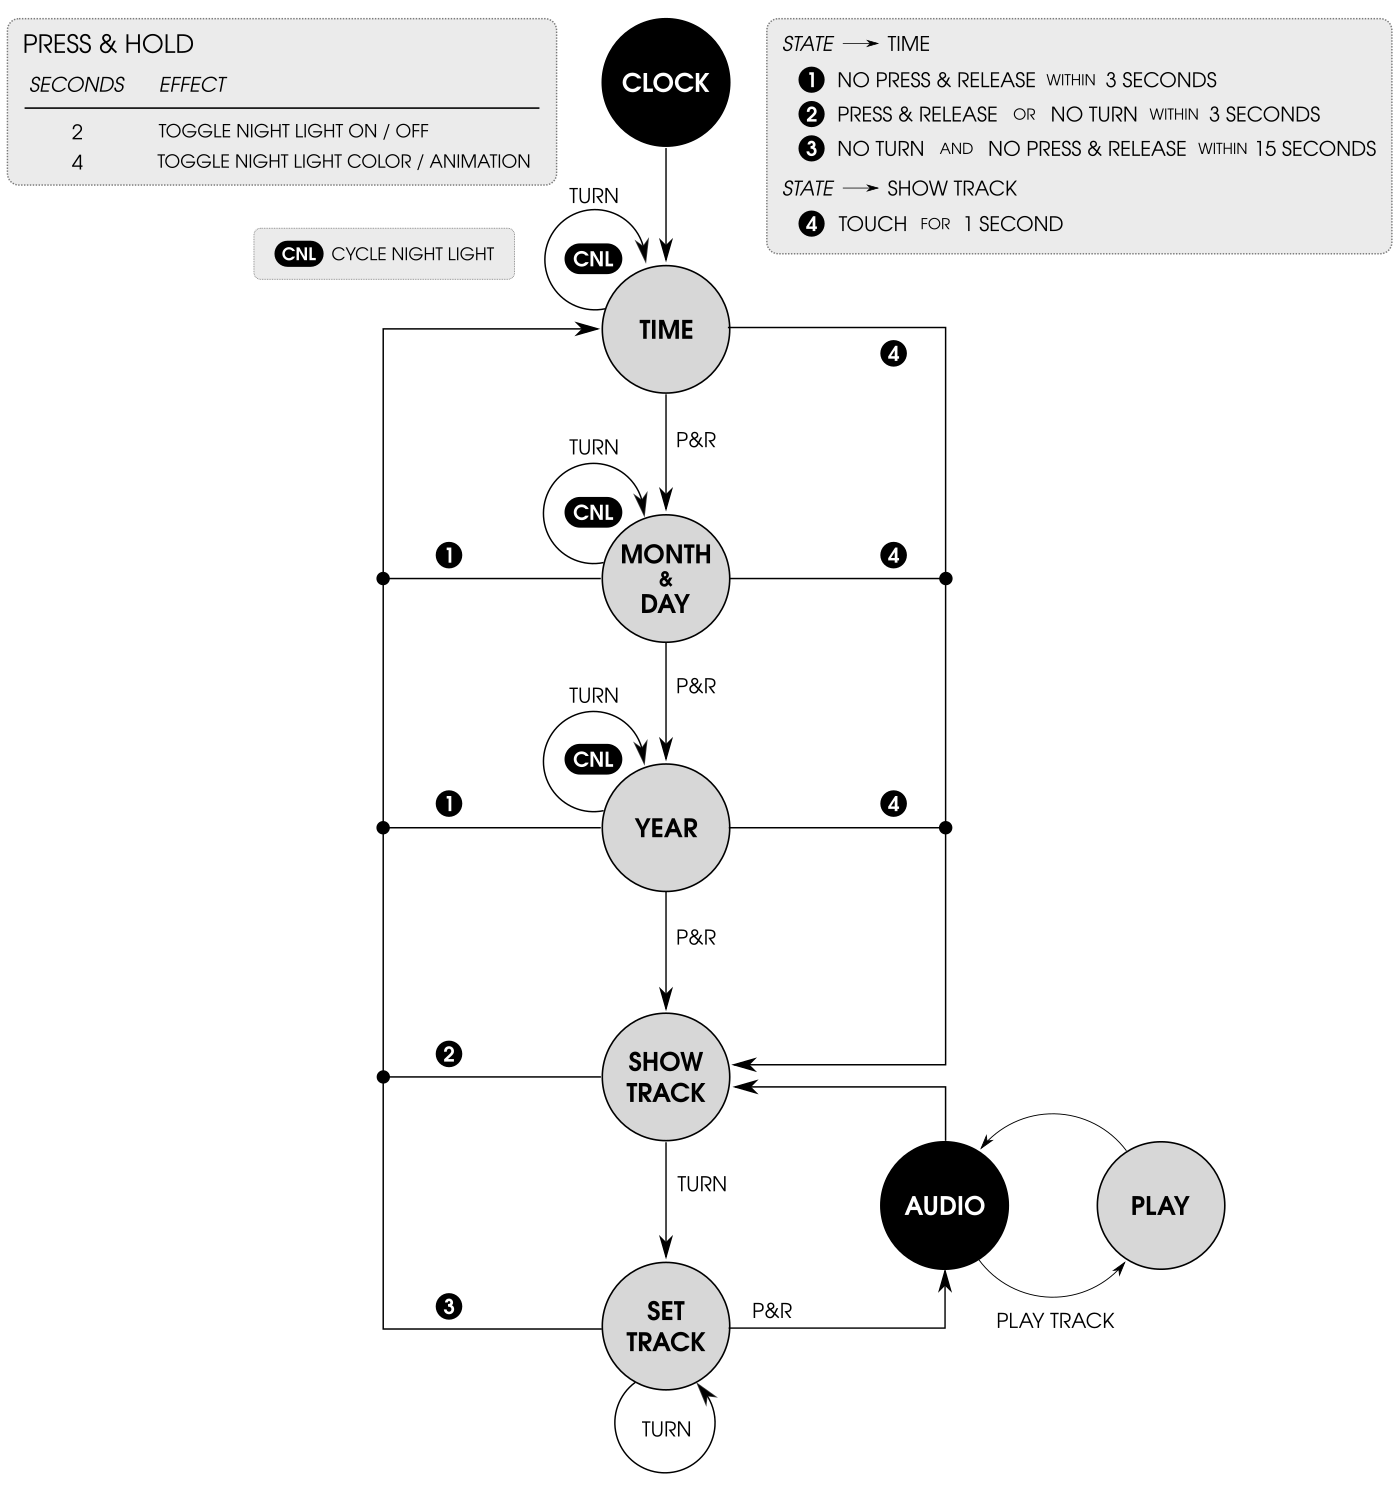
\includegraphics[]{images/clock_state_diagram.png}
\caption{Clock - State Diagram}
\end{figure}

%%%%%%%%%%%%%%%%%%%%%%%%%%%%%%%%%%%%%%%%%%%%%%%%%%%%%%%%%%%%%%%%%%%%%%%%%%%%%%%%
% Set Alarm
%%%%%%%%%%%%%%%%%%%%%%%%%%%%%%%%%%%%%%%%%%%%%%%%%%%%%%%%%%%%%%%%%%%%%%%%%%%%%%%%
\chapter{Set Alarm} \label{Set Alarm}
\vspace{-10ex}\mSA{syml}\vskip 8ex

%%%%%%%%%%%%%%%%%%%%%%%%%%%%%%%%%%%%%%%%%%%%%%%%%%%%%%%%%%%%%%%%%%%%%%%%%%%%%%%%
% Introduction
%%%%%%%%%%%%%%%%%%%%%%%%%%%%%%%%%%%%%%%%%%%%%%%%%%%%%%%%%%%%%%%%%%%%%%%%%%%%%%%%
\section{Introduction}

Allows setting a \textit{time of day} alarm where either the \cBe{f} or
\mAu{f} can be used as an alarm wakeup source.  Additionally it allows for
setting the amount of time the alarm will snooze as well as automatic off times
for when the alarm has been alerting or \sAlIP{f} for too long.  The time will
be displayed in either \num{12} or \num{24} hour format, whichever is used to
display the \mCl{f}.

\par\medskip

It is the \mPr{f} mode when the \cRs{f} is in the \dLe{f}
position.  See \hyperref[Alarm]{\mAl{f}} for more information on how the alarm
functions.

\par\medskip

There are a few ways to get to \mSA{f} depending on which direction the \cRs{f}
is pointing and which mode the device is currently in.

\begin{table}[H]
\ers{3}
\centering
\begin{tabu} { X[1,c,m] | X[1,c,m] | X[1,c,m] }
  \thrule
  \thbi{Position} & \thbi{Mode} & \thbi{Action} \\ \mrule

  \sMi & \multirow{2}{*}[-1mm]{\mode{s}{ANY}}
    & $\hskip -5mm$ \sMtoL \\ \dcrule{1}{1} \dcrule{3}{3}
  \sRi & & \sRtoL \\ \mdrule

  \multirow{4}{*}[-1.5mm]{\sLe}
    & \mSC{sym} & \sSec \\ \dcrule{2}{3}

  & \multirow{2}{*}[-1.5mm]{\mTS{sym}}
    & \sSec \\ \dcrule{3}{3}

  & & \sTer \\ \dcrule{2}{3}

  & \mode{f}{ANY} & \sLtoM \quad\quad \sMtoL \\

  \bhrule
\end{tabu}
\caption{Set Alarm - Mode}
\end{table}

\pagebreak

A few items of note:

\begin{itemize}
  \item All previously saved settings will initially be loaded.
  \item After setting the time of day, you can change mode, and the settings
    will be saved and the \mAl{f} will be set.  This allows for setting the time
    without having to go through the rest of the settings.
  \item To \aReset{f}, \aPH{f} the \cEs{f} until \symD{<<<<} is blinking on
    the \cDi{f}.
    \begin{enumerate}
      \item If the \aReset{f} is done from \sSAHo{f}, the alarm will be
        \sSADi{f} and display \symD{OFF!}.
      \item If done from any other state, it will start over from \sSAHo{f}.
    \end{enumerate}
  \item When the alarm is \sSADi{f}, \aPR{f} the \cEs{f} to enable the alarm.
\end{itemize}

%%%%%%%%%%%%%%%%%%%%%%%%%%%%%%%%%%%%%%%%%%%%%%%%%%%%%%%%%%%%%%%%%%%%%%%%%%%%%%%%
% Overview
%%%%%%%%%%%%%%%%%%%%%%%%%%%%%%%%%%%%%%%%%%%%%%%%%%%%%%%%%%%%%%%%%%%%%%%%%%%%%%%%
\section{Overview}

There are a number of states \mSA{f} can be in and are explained in the next
sections.

\begin{table}[H]
\ers{2}
\centering
\begin{tabu}{ X[1,c,m] | X[3,l,m] }
  \thrule

  \thbi{State} & \thbi{Description} \\ \mrule

  \sSAHo{sym} & Set the hour. \\ \drule{2}
  \sSAMi{sym} & Set the minute. \\ \drule{2}
  \sSAWS{sym} & Set the wakeup source - either \cBe{f} or \mAu{f}. \\ \drule{2}
  \sSAST{sym} & Set the amount of time the alarm will snooze. \\ \drule{2}
  \sSAWT{sym} & Set the amount of time the alarm can be alerting before
    automatically turning off. \\ \drule{2}
  \sSATT{sym} & Set the amount of time the alarm can be \sAlIP{f} 
                before automatically turning off. \\ \drule{2}
  \sSADo{sym} & Display alarm settings. \\ \drule{2}
  \sSADi{sym} & Alarm is disabled. \\
  \bhrule
\end{tabu}
\caption{Set Alarm - States}
\end{table}

\mSA{f} will initially start out in one of two states - \sSAHo{f} or \sSADi{f}.
If the alarm is \sSADi{f}, the display will show

\begin{figure}[H]
\centering
  \sDl{OFF!}
\end{figure}

and it will \textit{not} be blinking.  To enable the alarm, \aPR{f} the \cEs{f}.

\as{{c c c c}}{\sSADi{sym} & \sPR & \eEn{sym}{ALARM} & \sSAHo{sym} \\}

After being enabled, any previously saved settings will be in effect so you
do not need to reconfigure the alarm unless you want to change it.

\par\medskip

If you want to disable the alarm, from \sSAHo{f}, perform a \aReset{f}, i.e.
\aPH{f} the \cEs{f} until \symD{<<<<} is blinking on the display then \aRe{f}.

\as{{c c c c}}{\sSAHo{sym} & \sReset & \eDisable{sym}{ALARM} & \sSADi{sym} \\}

\info{The alarm can only be \sSADi{f} from the \sSAHo{f} state.  A \aReset{f} from
any other state will start over from the \sSAHo{f} state.}

\par\medskip

When enabled, to progress through the states, you will \aTu{f} the
\cEs{f} to select a value, then \aPR{f} the \cEs{f} to cache the setting and
move on to the next setting.

\tabcolsep=8pt
\as{{ c c c c c c c c c c c c c }}{%
\sSAHo{sym} & \sTu & \sPR & \sSAMi{sym} & \sTu & \sPR
  & \sSAWS{sym} & \sTu & \sPR & $\cdots$\quad$\cdots$
    & \sSADo{sym} & \sPR & \sSAHo{sym} \\}
\tabcolsep=12pt

When all settings have been configured, the \sSADo{f} state cycles through and
displays each one.  It will cycle repeatedly until you \aPR{f} the \cEs{f}.

\par\medskip

After setting and caching the \sSAMi{f}, you can short circuit the process by
changing mode and the alarm will be set and saved.

\tabcolsep=10pt
\ase{3}{{m{4.1in} m{0.8in} m{0.8in} m{1mm}}}{%
  \begin{tabu}{c c c c c c c}
    \sSAHo{sym} & \sTu & \sPR & \sSAMi{sym} & \sTu & \sPR & \sSAWS{sym}
  \end{tabu} &
  \begin{tabu}{c}
    \sSec \\ \drule{1} \sTer \\ \drule{1} $\hskip -5.5mm$ \sLtoM \\ \drule{1} \sLtoR
  \end{tabu} &
  {\ers{0.1} \begin{tabu}{c} \eSe{sym}{ALARM} \\ \eSa{sym}{ALARM} \end{tabu}} & \\}
\tabcolsep=12pt

%%%%%%%%%%%%%%%%%%%%%%%%%%%%%%%%%%%%%%%%%%%%%%%%%%%%%%%%%%%%%%%%%%%%%%%%%%%%%%%%
% Time
%%%%%%%%%%%%%%%%%%%%%%%%%%%%%%%%%%%%%%%%%%%%%%%%%%%%%%%%%%%%%%%%%%%%%%%%%%%%%%%%
\section{Time} \label{Set Alarm - Time}

Setting the alarm \textit{time of day} happens on one screen of the \cDi{f} and
is composed of two states - \sSAHo{f} and \sSAMi{f}. The current setting, first
\sSAHo{f}, then \sSAMi{f}, will be \textit{blinking}.  The time will be
displayed in the current format that was chosen in \hyperref[Set Clock]{\mSC{f}}.

\par\medskip

For \num{12} hour format, a \textit{decimal} at the \textit{lower right} of the
\cDi{f} is the \mono{PM} indicator.

\figDT{11:00}{11 AM}{11:00.}{11 PM}

A couple of examples in \num{12} and \num{24} hour format:

\begin{table}[H]
\ers{2.5}
\begin{tabu}{X[2,l,m] | X[1,c,m] | X[1,c,m]}
  \thrule
  & \thbi{12 Hour} & \thbi{24 Hour} \\ \mrule
  Seven in the Morning & \sDl{!7:00} & \sDl{07:00} \\ \drule{3}
  Seven (or 19:00) in the Evening & \sDl{!7:00.} & \sDl{19:00} \\
  \bhrule
\end{tabu}
\end{table}

%%%%%%%%%%%%%%%%%%%%%%%%%%%%%%%%%%%%%%%%%%%%%%%%%%%%%%%%%%%%%%%%%%%%%%%%%%%%%%%%
% Time - Hour
%%%%%%%%%%%%%%%%%%%%%%%%%%%%%%%%%%%%%%%%%%%%%%%%%%%%%%%%%%%%%%%%%%%%%%%%%%%%%%%%
\subsection{Hour} \sSAHo{syml}

Set the hour when the alarm will start.

\par\medskip

To select the \sSAHo{f}, \aTu{f} the \cEs{f} then \aPR{f} to cache the setting and
move on to \sSAMi{f}.

\as{{c c c c}}{%
\multirow{2}{*}{\sSAHo{sym}}
  & \sTu & \sPR & \multirow{2}{*}{\sSAMi{sym}} \\
& \eUp{sym}{} & \eCa{sym}{} & \\}

You can turn in either direction to get to the hour you want to set.  The hour
will wrap at the \num{0} and \num{23} hour marks if the current format is
\num{24} hour.

\begin{table}[H]
\ers{1}
\centering
\begin{tabu} { c c c }
  \mrule
  \sD{00:00} & \sCC & \sD{23:00} \\
  \mrule
\end{tabu}
\quad\quad\quad\quad
\begin{tabu} { c c c }
  \mrule
  \sD{23:00} & \sCl & \sD{00:00} \\
  \mrule
\end{tabu}
\end{table}

For \num{12} hour format, the transitions between \mono{AM} and \mono{PM} when
turning clockwise and counter-clockwise from \num{12} \mono{AM} back to
\num{12} \mono{AM} are shown below.

\ase{1}{{ c c c c c c c c}}{%
\sCl & \sD{12:00} & $\cdots$ & \sD{11:00} & \sD{12:00.}
  & $\cdots$ & \sD{11:00.} & \sD{12:00} \\ \drule{8}
\sCC & \sD{12:00} & \sD{11:00.} & $\cdots$ & \sD{12:00.}
  & \sD{11:00} & $\cdots$ & \sD{12:00} \\}

%%%%%%%%%%%%%%%%%%%%%%%%%%%%%%%%%%%%%%%%%%%%%%%%%%%%%%%%%%%%%%%%%%%%%%%%%%%%%%%%
% Time - Minute
%%%%%%%%%%%%%%%%%%%%%%%%%%%%%%%%%%%%%%%%%%%%%%%%%%%%%%%%%%%%%%%%%%%%%%%%%%%%%%%%
\pagebreak
\subsection{Minute} \sSAMi{syml}

Set the minute when the alarm will start.

\par\medskip

To select the \sSAMi{f}, \aTu{f} the \cEs{f} then \aPR{f} to cache the setting and
move on to \sSAWS{f}.

\as{{c c c c }}{%
\multirow{2}{*}{\sSAMi{sym}}
  & \sTu & \sPR & \multirow{2}{*}{\sSAWS{sym}} \\
& \eUp{sym}{} & \eCa{sym}{} & \\}

\info{At this point, after caching, you can \aTu{f} the \cRs{f} or change mode
and the alarm will be set and saved.}

%%%%%%%%%%%%%%%%%%%%%%%%%%%%%%%%%%%%%%%%%%%%%%%%%%%%%%%%%%%%%%%%%%%%%%%%%%%%%%%%
% Wakeup Source
%%%%%%%%%%%%%%%%%%%%%%%%%%%%%%%%%%%%%%%%%%%%%%%%%%%%%%%%%%%%%%%%%%%%%%%%%%%%%%%%
\section{Wakeup Source} \sSAWS{syml}

Set the wakeup source when the alarm alerts.

\par\medskip

Either the \cBe{f} or \mAu{f} can be chosen as a wakeup source when the alarm
starts or resumes from snoozing. 

\figDT{bEEP}{Wake to \cBe{ss}}{PLAY}{Wake to \mAu{ss}}

\info{%
If the \mAu{f} is \sAuOc{f} when the alarm starts, the \cBe{f}
will be used regardless of setting.
The \mAu{f} is considered \sAuOc{f} if either of the following are true:
\begin{itemize}
  \item \mAu{f} is in the \sAuPl{f} state, \textit{or}
  \item \cPl{f}, \cNe{f} or \cPr{f} push-buttons are being \action{f}{PRESSED}.
\end{itemize}}
To select the wakeup source, \aTu{f} the \cEs{f} then \aPR{f}
to cache the setting and move on to \sSAST{f}.

\as{{c c c c }}{%
\multirow{2}{*}{\sSAWS{sym}}
  & \sTu & \sPR & \multirow{2}{*}{\sSAST{sym}} \\
& \eUp{sym}{} & \eCa{sym}{} & \\}

%%%%%%%%%%%%%%%%%%%%%%%%%%%%%%%%%%%%%%%%%%%%%%%%%%%%%%%%%%%%%%%%%%%%%%%%%%%%%%%%
% Snooze Time
%%%%%%%%%%%%%%%%%%%%%%%%%%%%%%%%%%%%%%%%%%%%%%%%%%%%%%%%%%%%%%%%%%%%%%%%%%%%%%%%
\section{Snooze Time} \sSAST{syml}

Set the amount of time in \textit{minutes} the alarm will snooze.

\par\medskip

The \cDi{f} will show the following

\figD{Sn:10}{10 Minutes}

and the number on the \textit{right} side of the \textit{colon} will be
\textit{blinking}.  The time can be set from \num{1} to \num{59} minutes.

\par\medskip

To select the \sSAST{f} in minutes, \aTu{f} the \cEs{f} then \aPR{f}
to cache the setting and move on to \sSAWT{f}.

\as{{c c c c }}{%
\multirow{2}{*}{\sSAST{sym}}
  & \sTu & \sPR & \multirow{2}{*}{\sSAWT{sym}} \\
& \eUp{sym}{} & \eCa{sym}{} & \\}

%%%%%%%%%%%%%%%%%%%%%%%%%%%%%%%%%%%%%%%%%%%%%%%%%%%%%%%%%%%%%%%%%%%%%%%%%%%%%%%%
% Wake Time
%%%%%%%%%%%%%%%%%%%%%%%%%%%%%%%%%%%%%%%%%%%%%%%%%%%%%%%%%%%%%%%%%%%%%%%%%%%%%%%%
\section{Wake Time} \sSAWT{syml}

Set the amount of time in \textit{minutes} that the alarm can alert for, without
being snoozed or manually stopped, before automatically stopping the alarm.
Useful if you forget to stop the alarm so it doesn't beep or play music all day.

\info{%
Set to \num{0} to \action{f}{DISABLE} this setting - the alarm will
alert until manually snoozed, stopped or, if enabled, the \sSATT{f} is
exceeded.}

The \cDi{f} will show the following

\figDT{On:10}{10 Minutes}{On:!0}{Disabled}

and the number on the \textit{right} side of the \textit{colon} will be
\textit{blinking}.  The time can be set from
\num{0} to \num{59} minutes with the value \num{0} being \state{f}{DISABLED}.

\par\medskip

To select the \sSAWT{f} in minutes, \aTu{f} the \cEs{f} then \aPR{f}
to cache the setting and move on to \sSATT{f}.

\as{{c c c c }}{%
\multirow{2}{*}{\sSAWT{sym}}
  & \sTu & \sPR & \multirow{2}{*}{\sSATT{sym}} \\
& \eUp{sym}{} & \eCa{sym}{} & \\}

%%%%%%%%%%%%%%%%%%%%%%%%%%%%%%%%%%%%%%%%%%%%%%%%%%%%%%%%%%%%%%%%%%%%%%%%%%%%%%%%
% Total Alarm Time
%%%%%%%%%%%%%%%%%%%%%%%%%%%%%%%%%%%%%%%%%%%%%%%%%%%%%%%%%%%%%%%%%%%%%%%%%%%%%%%%
\section{Total Alarm Time} \sSATT{syml}

Set the total amount of time in \textit{hours} that the alarm can be active or
\sAlIP{f} for after starting before automatically stopping the alarm.
Useful if you just don't want to get up in the morning and would otherwise
indefinitely snooze it.

\info{%
Set to \num{0} to \action{f}{DISABLE} this setting - the alarm will
stay on, i.e. \sAlIP{f} until manually stopped or, if enabled, the \sSAWT{f}
is exceeded during alerting.}

The \cDi{f} will show the following

\figDT{A.t.:!2}{2 Hours}{A.t.:!0}{Disabled}

and the number on the \textit{right} side of the \textit{colon} will be
\textit{blinking}.  The time can be set from
\num{0} to \num{23} hours with the value \num{0} being \state{f}{DISABLED}.

\par\medskip

To select the \sSATT{f} in hours, \aTu{f} the \cEs{f} then \aPR{f} to finish.
At this point, the \mAl{f} is \textit{set and saved}.

\as{{c c c c c}}{%
\multirow{2}{*}{\sSATT{sym}}
  & \sTu & \multirow{2}{*}{\sPR} & \eSe{sym}{ALARM}
  & \multirow{2}{*}{\sSADo{sym}} \\
& \eUp{sym}{} & & \eSa{sym}{ALARM} & \\}

%%%%%%%%%%%%%%%%%%%%%%%%%%%%%%%%%%%%%%%%%%%%%%%%%%%%%%%%%%%%%%%%%%%%%%%%%%%%%%%%
% Done
%%%%%%%%%%%%%%%%%%%%%%%%%%%%%%%%%%%%%%%%%%%%%%%%%%%%%%%%%%%%%%%%%%%%%%%%%%%%%%%%
\section{Done} \sSADo{syml}

This state allows you to review the settings which are shown one by one on
the \cDi{f}.

\par\medskip

At this point you can start over or go to some other mode.  To start over and
go back to \sSAHo{f}, \aPR{f} the \cEs{f}.

\as{{c c c}}{\sSADo{sym} & \sPR & \sSAHo{sym} \\}

To go to, say \mCl{f} mode, \aTu{f} the \cRs{f} to the \dMi{f}.

\ase{3}{{c c c}}{\sSADo{sym} & \sLtoM & \mCl{sym} \\}

%%%%%%%%%%%%%%%%%%%%%%%%%%%%%%%%%%%%%%%%%%%%%%%%%%%%%%%%%%%%%%%%%%%%%%%%%%%%%%%%
% Disabled
%%%%%%%%%%%%%%%%%%%%%%%%%%%%%%%%%%%%%%%%%%%%%%%%%%%%%%%%%%%%%%%%%%%%%%%%%%%%%%%%
\section{Disabled} \sSADi{syml}

The alarm is disabled.

\par\medskip

When the alarm is \sSADi{f}, the display will show

\figD{OFF!}{Alarm Disabled}

and it will \textit{not} be blinking.  To enable the alarm, \aPR{f} the \cEs{f}.

\as{{c c c c}}{\sSADi{sym} & \sPR & \eEn{sym}{ALARM} & \sSAHo{sym} \\}

After being enabled, any previously saved settings will be in effect so you
do not need to reconfigure the alarm unless you want to change it.  If you
do want to change the alarm, see \hyperref[Set Alarm - Time]{Time}.

\par\medskip

To disable the alarm, from \sSAHo{f}, perform a \aReset{f}, i.e.
\aPH{f} the \cEs{f} until \symD{<<<<} is blinking on the display then \aRe{f}.

\as{{c c c c}}{\sSAHo{sym} & \sReset & \eDisable{sym}{ALARM} & \sSADi{sym} \\}

The alarm can only be \sSADi{f} from the \sSAHo{f} state.

%%%%%%%%%%%%%%%%%%%%%%%%%%%%%%%%%%%%%%%%%%%%%%%%%%%%%%%%%%%%%%%%%%%%%%%%%%%%%%%%
% Power
%%%%%%%%%%%%%%%%%%%%%%%%%%%%%%%%%%%%%%%%%%%%%%%%%%%%%%%%%%%%%%%%%%%%%%%%%%%%%%%%
\section{Power}

The screens will turn \sOff{f} when the device is in \sPoNa{f} or \sPoSl{f}
states.

\begin{table}[H]
\ers{2}
\begin{tabu}{ X[1,c,m] | X[1,c,m] | X[1,c,m] }
  \thrule
  \thbi{Power State} & \thbi{Set Alarm State} & \thbi{Screens} \\ \mrule
  \sPoNa{sym} & \multirow{2}{*}{\state{f}{ANY}}
    & \multirow{2}{*}{\sOff{sym}} \\ \dcrule{1}{1}
  \sPoSl{sym} & & \\
  \bhrule
\end{tabu}
\caption {Set Alarm - Power}
\end{table}

%%%%%%%%%%%%%%%%%%%%%%%%%%%%%%%%%%%%%%%%%%%%%%%%%%%%%%%%%%%%%%%%%%%%%%%%%%%%%%%%
% Reference
%%%%%%%%%%%%%%%%%%%%%%%%%%%%%%%%%%%%%%%%%%%%%%%%%%%%%%%%%%%%%%%%%%%%%%%%%%%%%%%%
\pagebreak
\section{Reference}

\ers{2.5}
\begin{longtabu}{ X[2,c,m] | X[1,c,m] | X[4,c,m] | X[2,c,m] }
  \thrule
  \thbi{State} & \thbi{Action} & \thbi{Effect} & \thbi{Next} \\ \mdrule

  & \sTu & \eUp{sym}{HOUR} & --- \\ \dcrule{2}{4}
  \sSAHo{sym} & \sPR & \eCa{sym}{HOUR} \eBl{sym}{MINUTE} & \sSAMi{sym} \\ \dcrule{2}{4}
  & \sReset & \eDisable{sym}{ALARM} \enspace \eDi{sym}{}\symD{OFF!} & \sSADi{sym} \\ \mrule

  \multirow{2}{*}[-1.5mm]{\sSAMi{sym}}
    & \sTu & \eUp{sym}{MINUTE} & --- \\ \dcrule{2}{4}
  & \sPR & \eCa{sym}{MINUTE} \eBl{sym}{WAKEUP SOURCE} & \sSAWS{sym} \\ \mrule

  \multirow{2}{*}[-1.5mm]{\sSAWS{sym}}
    & \sTu & \eUp{sym}{WAKEUP SOURCE} & --- \\ \dcrule{2}{4}
  & \sPR & \eCa{sym}{WAKEUP SRC} \eBl{sym}{SNOOZE TIME} & \sSAST{sym} \\ \mrule

  \multirow{2}{*}[-1.5mm]{\sSAST{sym}}
    & \sTu & \eUp{sym}{SNOOZE TIME} & --- \\ \dcrule{2}{4}
  & \sPR & \eCa{sym}{SNOOZE TIME} \eBl{sym}{WAKE TIME} & \sSAWT{sym} \\ \mrule

  \multirow{2}{*}[-1.5mm]{\sSAWT{sym}}
    & \sTu & \eUp{sym}{WAKE TIME} & --- \\ \dcrule{2}{4}
  & \sPR & \eCa{sym}{WAKE TIME} \eBl{sym}{TOTAL ALARM TIME} & \sSATT{sym} \\ \mrule

  \multirow{2}{*}[-1.5mm]{\sSATT{sym}}
    & \sTu & \eUp{sym}{TOTAL ALARM TIME} & --- \\ \dcrule{2}{4}
  & \sPR & \eSe{sym}{ALARM} \eSa{sym}{ALARM} \eDi{sym}{ALARM} & \sSADo{sym} \\ \mrule

  \sSADo{sym} & \sPR & \eBl{sym}{HOUR} & \sSAHo{sym} \\ \mrule

  \pagebreak
  \mrule

  \multirow{2}{*}[-1mm]{\sSADi{sym}} & \sPR
    & \multirow{2}{*}[-1mm]{\eEn{sym}{ALARM} \eBl{sym}{HOUR}}
    & \multirow{2}{*}[-1mm]{\sSAHo{sym}} \\ \dcrule{2}{2}
  & \sReset & & \\ \mrule

  {\ers{0.1} \tabcolsep=0pt
    \begin{tabu}{c} \sSAMi{sym} \\ \sSAWS{sym} \\ \sSAST{sym} \\
      \sSAWT{sym} \\ \sSATT{sym} \\ \sSADo{sym} \end{tabu} \tabcolsep=12pt}
    & \sReset & \eRe{sym}{} \eBl{sym}{HOUR} & \sSAHo{sym} \\ \mrule

  %\pagebreak
  %\mrule

  \multirow{4}{*}[-4mm]{\ers{0.1}\begin{tabu}{c}\sSAHo{sym}\\\sSAMi{sym}\\
      \enspace\sSADo{sym}\thinspace
      \footnote{ The alarm has already been set when \sSADo{ss}.}\\\sSADi{sym}\end{tabu}}
    & \sSec & \multirow{4}{*}[5mm]{\eCM{sym}} & \mSC{sym} \\ \dcrule{2}{2} \dcrule{4}{4}
    & \sTer & & \mTS{sym} \\ \dcrule{2}{2} \dcrule{4}{4}
    & $\hskip -5mm$ \sLtoM & & \mCl{sym} \\ \dcrule{2}{2} \dcrule{4}{4}
    & \sLtoR & & \mTi{sym} \\ \mrule

  \multirow{4}{*}[-7mm]{%
    \ers{0.1}\begin{tabu}{c}\sSAWS{sym}\\\sSAST{sym}\\\sSAWT{sym}\\\sSATT{sym}\end{tabu}}
    & \sSec & \multirow{4}{*}{\eSe{sym}{ALARM} \eSa{sym}{ALARM} \eCM{sym}}
      & \mSC{sym} \\ \dcrule{2}{2} \dcrule{4}{4}
    & \sTer & & \mTS{sym} \\ \dcrule{2}{2} \dcrule{4}{4}
    & $\hskip -5mm$ \sLtoM & & \mCl{sym} \\ \dcrule{2}{2} \dcrule{4}{4}
    & \sLtoR & & \mTi{sym} \\

  \bhrule
  \caption {Set Alarm - Reference}
\end{longtabu}

%%%%%%%%%%%%%%%%%%%%%%%%%%%%%%%%%%%%%%%%%%%%%%%%%%%%%%%%%%%%%%%%%%%%%%%%%%%%%%%%
% State Diagram
%%%%%%%%%%%%%%%%%%%%%%%%%%%%%%%%%%%%%%%%%%%%%%%%%%%%%%%%%%%%%%%%%%%%%%%%%%%%%%%%
%\pagebreak
\section{State Diagram} \label{Set Alarm State Diagram}

\begin{figure}[H]
  \centering
  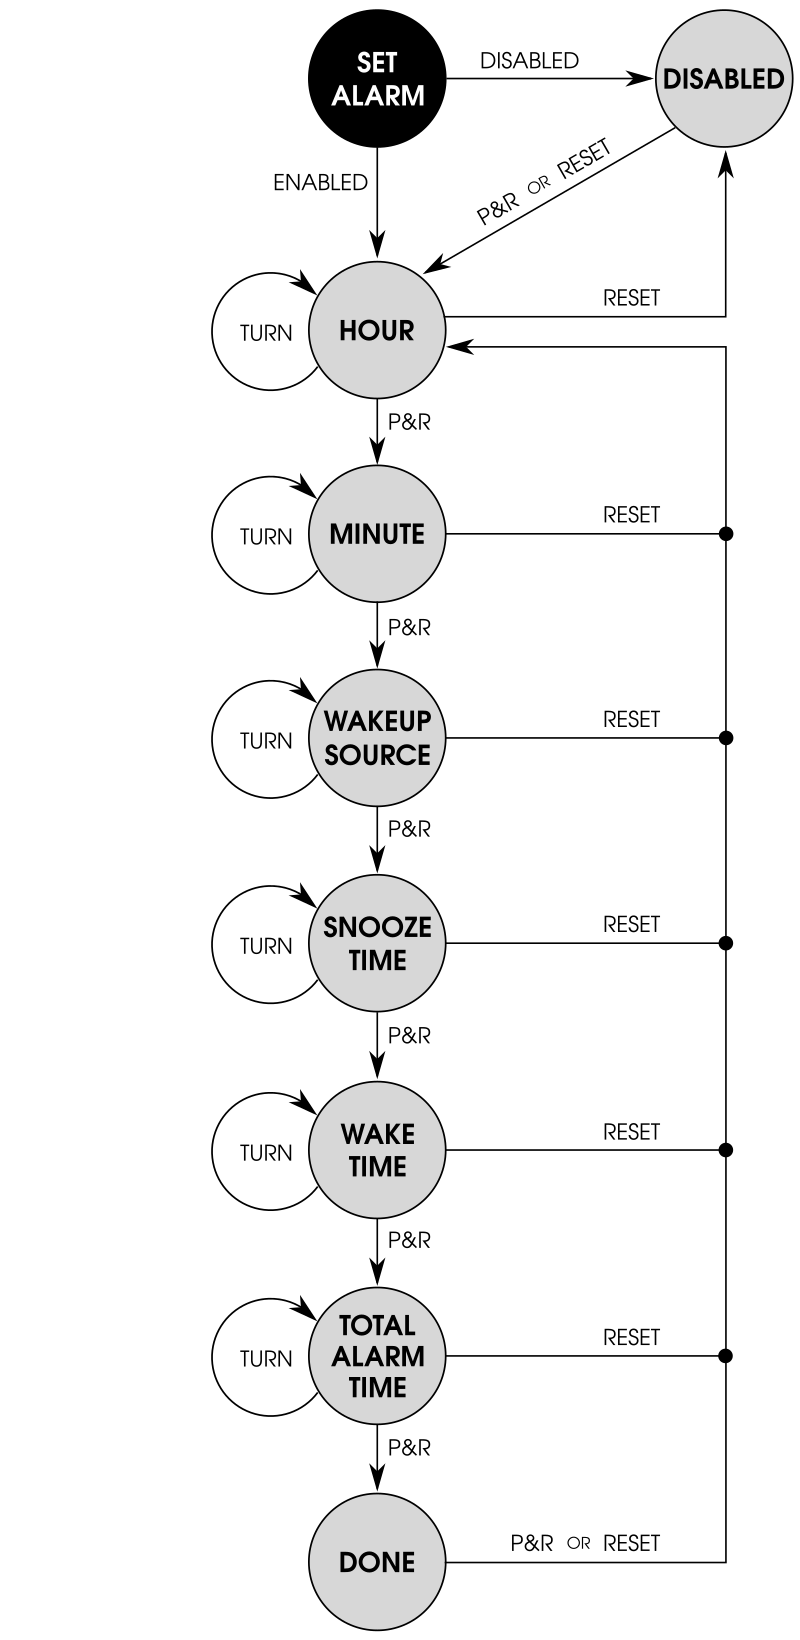
\includegraphics{images/set_alarm_state_diagram.png}
  \caption{Set Alarm - State Diagram}
\end{figure}

%%%%%%%%%%%%%%%%%%%%%%%%%%%%%%%%%%%%%%%%%%%%%%%%%%%%%%%%%%%%%%%%%%%%%%%%%%%%%%%%
% Timer
%%%%%%%%%%%%%%%%%%%%%%%%%%%%%%%%%%%%%%%%%%%%%%%%%%%%%%%%%%%%%%%%%%%%%%%%%%%%%%%%
\chapter{Timer} \label{Timer}
\vspace{-10ex}\mTi{syml}\vskip 8ex

%%%%%%%%%%%%%%%%%%%%%%%%%%%%%%%%%%%%%%%%%%%%%%%%%%%%%%%%%%%%%%%%%%%%%%%%%%%%%%%%
% Introduction
%%%%%%%%%%%%%%%%%%%%%%%%%%%%%%%%%%%%%%%%%%%%%%%%%%%%%%%%%%%%%%%%%%%%%%%%%%%%%%%%
\section{Introduction}

Allows setting and running a timer.  The timer can be set anywhere from \num{1}
second to \num{99} hours and \num{99} minutes, can be paused using the \cEs{f}
and alerts when the timer expires using the \cBe{f} that can be turned off using
either the \cEs{f} or \aTo{f}.

\par\medskip

There is also the option, by touching the top of the enclosure for \num{1}
second, to toggle the use of the \cLi{f} window as a display of colors that
change as the timer counts down giving a visual indication as to the approximate
time left.

\par\medskip

The clock can also be displayed while the timer is active by using the \cEs{f}.

\par\medskip

There are a few ways to get to \mTi{f} mode depending on which direction the
\cRs{f} is pointing and which mode the device is currently in.

\ers{2.3}
\begin{table}[H]
  \centering
  \begin{tabu} { X[1,c,m] | X[1,c,m] | X[1,c,m] }
    \thrule
    \thbi{Position} & \thbi{Mode} & \thbi{Action} \\ \mrule

    \sLe & \multirow{2}{*}[-1mm]{\mode{s}{ANY}} & \sLtoR \\ \dcrule{1}{1} \dcrule{3}{3}
    \sMi & & $\hskip 4mm$ \sMtoR \\ \mdrule

    \multirow{4}{*}[-9mm]{\sRi}
      & \mPS{sym} & \sSec \\ \dcrule{2}{3}

    & \multirow{2}{*}[-1.5mm]{\mSN{sym}}
      & \sSec \\ \dcrule{3}{3}
    & & \sTer \\ \dcrule{2}{3}

    & \mode{f}{ANY} & \sRtoM \quad\quad \sMtoR \\

    \bhrule
  \end{tabu}
  \caption{Timer - Mode}
\end{table}

%%%%%%%%%%%%%%%%%%%%%%%%%%%%%%%%%%%%%%%%%%%%%%%%%%%%%%%%%%%%%%%%%%%%%%%%%%%%%%%%
% Overview
%%%%%%%%%%%%%%%%%%%%%%%%%%%%%%%%%%%%%%%%%%%%%%%%%%%%%%%%%%%%%%%%%%%%%%%%%%%%%%%%
\section{Overview}

There are a number of states \mTi{f} can be in and are explained in the next
sections.

\ers{2}
\begin{table}[H]
  \centering
  \begin{tabu} { X[1,c,m] | X[3,l,m] }
    \thrule
    \thbi{State} & \thbi{Description} \\ \mrule

    \sTiHM{sym} & Set hours | minutes field. \\ \drule{2}
    \sTiMS{sym} & Set minutes if \sTiHM{f} is in hours or
      seconds if in minutes.  \\ \drule{2}
    \sTiRu{sym} & Timer is actively counting down.  \\ \drule{2}
    \sTiPa{sym} & Timer countdown is paused.  \\ \drule{2}
    \sTiAl{sym} & Timer expired and is alerting\slash beeping.  \\ \drule{2}
    \sTiWa{sym} & State after alerting is stopped or first state if
        a time has previously been set. \\
    \bhrule
  \end{tabu}
  \caption{Timer - States}
\end{table}

The first time \mTi{f} is entered after the device is switched \sOn{f}, the
time will have to be set and the first state will be \sTiHM{f}.  The general
progression involves first, setting the time, after which the timer starts
running, then letting the timer count down to \num{0} at which time it begins
alerting, and then stopping the alerting by either \action{f}{TURNING} the
\cEs{f} or \action{f}{TOUCHING} the \control{f}{TOP} of the enclosure.

\tabcolsep=10pt
\ase{1}{{c c c c c c c c c c c}}{%
\multirow{2}{*}{\sTiHM{sym}}
  & \multirow{2}{*}{\sTu}
  & \multirow{2}{*}{\sPR}
  & \multirow{2}{*}{\sTiMS{sym}}
  & \multirow{2}{*}{\sTu}
  & \multirow{2}{*}{\sPR}
  & \multirow{2}{*}{\sTiRu{sym}}
  & \multirow{2}{*}{\eAc{sym}{TIMER EXPIRES}}
  & \multirow{2}{*}{\sTiAl{sym}}
  & \sPR
  & \multirow{2}{*}{\sTiWa{sym}} \\ \dcrule{10}{10}
& & & & & & & & & \sTo & \\}
\tabcolsep=12pt

\info{For touch to work, make sure you have enabled it via
\hyperref[Touch Settings]{\mTS{f}} and that the palm of your hand or
most of your fingers touch the top of the enclosure - it won't likely be enough
to just touch or tap the top with one finger.}

Subsequent entries into \mTi{f} mode will load the previously set time and the
first state will be \sTiWa{f}\footnote{ The time isn't saved when the device is
powered \sOff{f} via the \cPo{ss} switch, so each time the device is powered
\sOn{f} it will start in \sTiHM{ss} state and you will have to set the time.}
from which you can either start the timer by pressing and releasing the \cEs{f}.

\as{{c c c c c}}{\mTi{sym} & \sTiWa{sym} & \sPR & \sTiRu{sym} & $\cdots$ \\}

or set a new time by turning the \cEs{f}.

\as{{c c c c c}}{\mTi{sym} & \sTiWa{sym} & \sTu & \sTiMS{sym} & $\cdots$ \\}

When the timer is running, you can \sTiPa{f} it by a \aPR{f} of the \cEs{f}.
To resume, \aPR{f} again.

\as{{c c c c c c}}{\sTiRu{sym} & \sPR & \sTiPa{sym} & \sPR & \sTiRu{sym} & $\cdots$ \\}

%%%%%%%%%%%%%%%%%%%%%%%%%%%%%%%%%%%%%%%%%%%%%%%%%%%%%%%%%%%%%%%%%%%%%%%%%%%%%%%%
% Set Time
%%%%%%%%%%%%%%%%%%%%%%%%%%%%%%%%%%%%%%%%%%%%%%%%%%%%%%%%%%%%%%%%%%%%%%%%%%%%%%%%
\section{Set Time}

Setting the time occurs on one screen of the \cDi{f} and is composed of two
states - \sTiHM{f} and \sTiMS{f}. The current setting, first \sTiHM{f}, then
\sTiMS{f}, will be \textit{blinking}.  The time can be set anywhere from \num{1}
second to \num{99} hours and \num{99} minutes.

\figDT{00:01}{1 Second}{99:99.}{99 Hours \& 99 Minutes}

To the \textit{left} of the \textit{colon} is where you set the minutes or if
more than \num{59} minutes, the hours.  As you \aTu{f} the \cEs{f}
\textit{clockwise} the number will increase until it hits \num{59} minutes at
which point it will change over to hours and display a \textit{decimal} in the
\textit{lower right} of the \cDi{f}.  The decimal indicates that the time is in
hours and minutes or \mono{HH:MM}.

\figDT{59:00}{59 Minutes}{!1:00.}{1 Hour}

Like other options, the numbers in the fields will wrap.  Below shows the basic
milestones as you turn in one direction or the other when in \sTiHM{f}.

\ase{1}{{c c c c c c c c}}{%
\sCl & \sD{!0:00} & $\cdots$ & \sD{59:00}
  & \sD{!1:00.} & $\cdots$ & \sD{99:00.} & \sD{!0:00} \\ \drule{8}
\sCC & \sD{!0:00} & \sD{99:00.} & $\cdots$
  & \sD{!1:00.} & \sD{59:00} & $\cdots$ & \sD{!0:00} \\}

%%%%%%%%%%%%%%%%%%%%%%%%%%%%%%%%%%%%%%%%%%%%%%%%%%%%%%%%%%%%%%%%%%%%%%%%%%%%%%%%
% Set Time - Set H|M
%%%%%%%%%%%%%%%%%%%%%%%%%%%%%%%%%%%%%%%%%%%%%%%%%%%%%%%%%%%%%%%%%%%%%%%%%%%%%%%%
\subsection{Set Hours or Minutes} \sTiHM{syml}

Set the hours or minutes.

\par\medskip

To select the hours or minutes, \aTu{f} the \cEs{f} then \aPR{f} to cache the
setting and move on to \sTiMS{f}.

\as{{c c c c}}{%
\multirow{2}{*}{\sTiHM{sym}}
  & \sTu & \sPR & \multirow{2}{*}{\sTiMS{sym}} \\
& \eUp{sym}{} & \eCa{sym}{} & \\}

%%%%%%%%%%%%%%%%%%%%%%%%%%%%%%%%%%%%%%%%%%%%%%%%%%%%%%%%%%%%%%%%%%%%%%%%%%%%%%%%
% Set Time - Set M|S
%%%%%%%%%%%%%%%%%%%%%%%%%%%%%%%%%%%%%%%%%%%%%%%%%%%%%%%%%%%%%%%%%%%%%%%%%%%%%%%%
\subsection{Set Minutes or Seconds} \sTiMS{syml}

Set the minutes or seconds.

\par\medskip

To select the minutes or seconds, \aTu{f} the \cEs{f} then \aPR{f} to start the
timer.

\as{{c c c c}}{%
\multirow{2}{*}{\sTiMS{sym}}
  & \sTu & \sPR & \multirow{2}{*}{\sTiRu{sym}} \\
& \eUp{sym}{} & \eStart{sym}{TIMER} & \\}

%%%%%%%%%%%%%%%%%%%%%%%%%%%%%%%%%%%%%%%%%%%%%%%%%%%%%%%%%%%%%%%%%%%%%%%%%%%%%%%%
% Run
%%%%%%%%%%%%%%%%%%%%%%%%%%%%%%%%%%%%%%%%%%%%%%%%%%%%%%%%%%%%%%%%%%%%%%%%%%%%%%%%
\section{Run} \sTiRu{syml}

Timer is actively counting down.

\par\medskip

As the timer is actively counting down, the \cDi{f} is updated every second.

\begin{itemize}[leftmargin=*]
  \item If the time left is \textit{less} than \num{1} hour, the time will be
    formatted as minutes and seconds - \mono{MM:SS} - and progress can easily be
    seen as the seconds count down.
  \item Otherwise, when the time left is \num{1} hour or greater, since the time
    will be formatted as hours and minutes - \mono{HH:MM} - the \textit{decimal}
    in the \textit{lower right} of the \cDi{f} will \textit{blink} on and off
    every second to give an indication of progress.
\end{itemize}

To stop the timer before it has finished counting down, perform a \aReset{f},
i.e. \aPH{f} the \cEs{s} until \symD{<<<<} is blinking on the \cDi{f}.  This
can also be done in the \sTiPa{f} state.

\ase{1}{{c c c c}}{%
\sTiRu{sym} & \multirow{2}{*}{\sReset}
  & \multirow{2}{*}{\eSt{sym}{TIMER}}
  & \multirow{2}{*}{\sTiWa{sym}} \\ \dcrule{1}{1}
\sTiPa{sym} & & & \\}

When the timer expires, it will begin alerting with the \cBe{f}.

\ase{1}{{c c c c}}{\sTiRu{sym} & \eAc{sym}{TIMER EXPIRES} & \sTiAl{sym} \\}

%%%%%%%%%%%%%%%%%%%%%%%%%%%%%%%%%%%%%%%%%%%%%%%%%%%%%%%%%%%%%%%%%%%%%%%%%%%%%%%%
% Run - Lighting
%%%%%%%%%%%%%%%%%%%%%%%%%%%%%%%%%%%%%%%%%%%%%%%%%%%%%%%%%%%%%%%%%%%%%%%%%%%%%%%%
\subsection{Lighting} \label{Timer - Lighting}

The \cLi{f} window will be lit and progress seamlessly through the following
primary hues as the timer counts down giving a visual indication as to the
approximate time left.

\begin{table}[H] \ers{0.1} \begin{tabu} { c }
\cBl \cGr \cYe \cOr \cRe
\end{tabu} \end{table}

This is useful if you are some distance from the device and can't see the time
on the \cDi{f} or in a dimly lit or dark area and not facing the \cDi{f}.
However, if you don't want the lighting on while the timer is counting down,
it can be turned off.

\par\medskip

To toggle between showing and not showing the colors in the \cLi{f} window,
\aTo{f} the \cTo{f} of the enclosure for \num{1} second.  This can also be done
in the \sTiPa{f} state.

\ase{1}{{c c c}}{%
\sTiRu{sym} & \multirow{2}{*}{\sToN{1}}
  & \multirow{2}{*}{\eTo{sym}{LIGHTING ON|OFF}} \\ \dcrule{1}{1}
\sTiPa{sym} & & \\}

\info{For touch to work, make sure you have enabled it via
\hyperref[Touch Settings]{\mTS{f}} and that the palm of your hand or most of
your fingers lay on top of the enclosure.}

%%%%%%%%%%%%%%%%%%%%%%%%%%%%%%%%%%%%%%%%%%%%%%%%%%%%%%%%%%%%%%%%%%%%%%%%%%%%%%%%
% Pause
%%%%%%%%%%%%%%%%%%%%%%%%%%%%%%%%%%%%%%%%%%%%%%%%%%%%%%%%%%%%%%%%%%%%%%%%%%%%%%%%
\section{Pause} \sTiPa{syml}

Timer is paused.

\par\medskip

When the timer is counting down, i.e. in the \sTiRu{f} state, you can pause it.
To toggle between the \sTiRu{f} and \sTiPa{f} states, \aPR{f} the \cEs{f}.

\as{{c c c c c}}{%
\multirow{2}{*}{\sTiRu{sym}}
  & \sPR & \multirow{2}{*}{\sTiPa{sym}} & \sPR & \multirow{2}{*}{\sTiRu{sym}} \\
& \ePa{sym}{TIMER} & & \eResume{sym}{TIMER} & \\}

%%%%%%%%%%%%%%%%%%%%%%%%%%%%%%%%%%%%%%%%%%%%%%%%%%%%%%%%%%%%%%%%%%%%%%%%%%%%%%%%
% Alert
%%%%%%%%%%%%%%%%%%%%%%%%%%%%%%%%%%%%%%%%%%%%%%%%%%%%%%%%%%%%%%%%%%%%%%%%%%%%%%%%
\section{Alert} \sTiAl{syml}

The timer has expired and is alerting.

\par\medskip

When the timer expires, the \cBe{f} will alert and both the \cDi{f} and \cLi{f}
will blink in sync. The \cLi{f} window will blink red if it hasn't been turned
off and the \cDi{f} will blink

\begin{figure}[H]
\centering
  \sDl{donE}
\end{figure}

You can either \aPR{f} the \cEs{f} or \aTo{f} the \cTo{f} of the enclosure to
stop the alerting.  After the alerting is stopped, the \mTi{f} will go to the
\sTiWa{f} state.

\ase{1}{{c c c c}}{%
\multirow{2}{*}{\sTiAl{sym}} & \sPR
  & \multirow{2}{*}{\eSt{sym}{ALERTING}}
  & \multirow{2}{*}{\sTiWa{sym}} \\ \dcrule{2}{2}
& \sTo & & \\}

%%%%%%%%%%%%%%%%%%%%%%%%%%%%%%%%%%%%%%%%%%%%%%%%%%%%%%%%%%%%%%%%%%%%%%%%%%%%%%%%
% Wait
%%%%%%%%%%%%%%%%%%%%%%%%%%%%%%%%%%%%%%%%%%%%%%%%%%%%%%%%%%%%%%%%%%%%%%%%%%%%%%%%
\section{Wait} \sTiWa{syml}

Wait for user input.

\par\medskip

This is the state the \mTi{f} enters after \sTiAl{f} or from \sTiRu{f},
\sTiPa{f} or \sTiAl{f} when \aReset{f}.  Also, if you have previously set a
time, it will be the first state upon reentering \mTi{f} mode.

\par\medskip

If you don't need to update the time, \aPR{f} the \cEs{f} and the timer will
start counting down and be in the \sTiRu{f} state.

\as{{c c c}}{%
\multirow{2}{*}{\sTiWa{sym}}
  & \sPR & \multirow{2}{*}{\sTiRu{sym}} \\
& \eStart{sym}{TIMER} & \\}

If you want to adjust the time, \aTu{f} the \cEs{f}.

\as{{c c c}}{\sTiWa{sym} & \sTu & \sTiHM{sym} \\}

%%%%%%%%%%%%%%%%%%%%%%%%%%%%%%%%%%%%%%%%%%%%%%%%%%%%%%%%%%%%%%%%%%%%%%%%%%%%%%%%
% Show Clock
%%%%%%%%%%%%%%%%%%%%%%%%%%%%%%%%%%%%%%%%%%%%%%%%%%%%%%%%%%%%%%%%%%%%%%%%%%%%%%%%
\section{Show Clock}

When in \sTiRu{f} or \sTiPa{f} states the \cDi{f} can toggle between showing the
clock time and timer countdown time. To toggle between the two, \aTu{f} the
\cEs{f} at least \num{3} \textit{detents} quickly either clockwise or
counter-clockwise.

\ase{1}{{c c c}}{%
\sTiRu{sym}
  & \multirow{2}{*}{\sTuN{3}}
  & \multirow{2}{*}{\eTo{sym}{SHOW CLOCK|TIMER}} \\ \dcrule{1}{1}
\sTiPa{sym} & & \\}

Really just a quick \aTu{f} in either direction will work.  The timer will
continue to count down and the \cLi{f} window will continue to change color in
either case, so when the clock time is displayed, you can still get a feel for
the amount of timer time left by the color in the \cLi{f} window.  When the
timer expires, it will go into the \sTiAl{f} state which will take over the
\cDi{f}.

%%%%%%%%%%%%%%%%%%%%%%%%%%%%%%%%%%%%%%%%%%%%%%%%%%%%%%%%%%%%%%%%%%%%%%%%%%%%%%%%
% Power
%%%%%%%%%%%%%%%%%%%%%%%%%%%%%%%%%%%%%%%%%%%%%%%%%%%%%%%%%%%%%%%%%%%%%%%%%%%%%%%%
\section{Power}

The screens will either \sScDi{f} or turn \sScOf{f} depending on the current
state.  If the \mTi{f} is in either \sTiRu{f} or \sTiAl{f} states, the screens
will \sDim{f} for both \sPoNa{f} and \sPoSl{f} states, however, the device will
\textit{not} go to sleep - it will instead \sPoNa{f}.  For the other \mTi{f}
states, the screens will turn \sOff{f} in both \sPoNa{f} and \sPoSl{f} power
states.

\begin{table}[H]
\ers{2}
\begin{tabu}{ X[1,c,m] | X[1,c,m] | X[1,c,m] }
  \thrule
  \thbi{Power State} & \thbi{Timer State} & \thbi{Screens} \\ \mrule

  \multirow{2}{*}[-1mm]{\sPoNa{sym}}
    & \sTiRu{sym} \sTiAl{sym} & \sDim{sym} \\ \dcrule{2}{3}
  & \sTiHM{sym} \sTiMS{sym} \sTiPa{sym} \sTiWa{sym} & \sOff{sym} \\ \mrule

  \sPoSl{sym} $\rightarrow$ \sPoNa{sym} & \sTiRu{sym} \sTiAl{sym} & \sDim{sym} \\ \mrule
  \sPoSl{sym} & \sTiHM{sym} \sTiMS{sym} \sTiPa{sym} \sTiWa{sym} & \sOff{sym} \\

  \bhrule
\end{tabu}
\caption {Timer - Power}
\end{table}

%%%%%%%%%%%%%%%%%%%%%%%%%%%%%%%%%%%%%%%%%%%%%%%%%%%%%%%%%%%%%%%%%%%%%%%%%%%%%%%%
% Reference
%%%%%%%%%%%%%%%%%%%%%%%%%%%%%%%%%%%%%%%%%%%%%%%%%%%%%%%%%%%%%%%%%%%%%%%%%%%%%%%%
\section{Reference}

\ers{2.4}
\begin{longtabu}{ X[2,c,m] | X[1,c,m] | X[4,c,m] | X[2,c,m] }
  \thrule
  \thbi{State} & \thbi{Action} & \thbi{Effect} & \thbi{Next} \\ \hline

  \multirow{2}{*}[-1.5mm]{\sTiHM{sym}}
    & \sTu & \eUp{sym}{H|M} & --- \\ \dcrule{2}{4}
  & \sPR & \eBl{sym}{M|S} & \sTiMS{sym} \\ \mrule

  \multirow{2}{*}[-1.5mm]{\sTiMS{sym}}
    & \sTu & \eUp{sym}{M|S} & --- \\ \dcrule{2}{4}
  & \sPR & \eStart{sym}{TIMER} & \sTiRu{sym} \\ \mrule

  \multirow{4}{*}[-1.5mm]{\sTiRu{sym}}
    & \sPR & \ePa{sym}{TIMER} & \sTiPa{sym} \\ \dcrule{2}{4}
  & $\hskip 1.2mm$ \sTuN{3} & \eTo{sym}{SHOW CLOCK|TIMER} & --- \\ \dcrule{2}{4}
  & $\hskip 1.2mm$ \sToN{1}
    & \eTo{sym}{LIGHTING ON|OFF} & --- \\ \dcrule{2}{4}
  & \action{ss}{TIMER EXPIRES} & \eAl{sym} \eBl{sym}{DONE} & \sTiAl{sym} \\ \mrule

  \pagebreak
  \mrule

  \multirow{3}{*}[-1.5mm]{\sTiPa{sym}}
    & \sPR & \eResume{sym}{TIMER} & \sTiRu{sym} \\ \dcrule{2}{4}
  & $\hskip 1.2mm$ \sTuN{3} & \eTo{sym}{SHOW CLOCK|TIMER} & --- \\ \dcrule{2}{4}
  & $\hskip 1.2mm$ \sToN{1}
    & \eTo{sym}{LIGHTING ON|OFF} & --- \\ \mrule

  \multirow{2}{*}[-1.5mm]{\sTiAl{sym}}
    & \sPR & \multirow{2}{*}[-1.5mm]{\eSt{sym}{ALERTING} \eDi{sym}{TIME}}
      & \multirow{2}{*}[-1.5mm]{\sTiWa{sym}} \\ \dcrule{2}{2}
    & \sTo & & \\ \mrule

  \multirow{2}{*}[-1.5mm]{\sTiWa{sym}}
    & \sPR & \eStart{sym}{TIMER} & \sTiRu{sym} \\ \dcrule{2}{4}
    & \sTu & \eBl{sym}{H|M} & \sTiHM{sym} \\ \mrule

  \sTiHM{sym} \sTiMS{sym} \newline \sTiWa{sym}
    & \multirow{2}{*}[-1.5mm]{\sReset} & \eRe{sym}{} \eBl{sym}{H|M} & \sTiHM{sym}
      \\ \dcrule{1}{1} \dcrule{3}{4}
  \sTiRu{sym} \sTiPa{sym} \sTiAl{sym} & & \eSt{sym}{TIMER} \eDi{sym}{TIME} & \sTiWa{sym}
  \\ \mrule

  \multirow{4}{*}[-1.5mm]{\state{f}{ANY}}
    & \sSec & \multirow{4}{*}[-1.5mm]{\eCM{sym}} & \mPS{sym} \\ \dcrule{2}{2} \dcrule{4}{4}
  & \sTer & & \mSN{sym} \\ \dcrule{2}{2} \dcrule{4}{4}
  & $\hskip 3mm$ \sRtoM & & \mCl{sym} \\ \dcrule{2}{2} \dcrule{4}{4}
  & \sRtoL & & \mSA{sym} \\

  \bhrule
\caption{Timer - Reference}
\end{longtabu}

%%%%%%%%%%%%%%%%%%%%%%%%%%%%%%%%%%%%%%%%%%%%%%%%%%%%%%%%%%%%%%%%%%%%%%%%%%%%%%%%
% State Diagram
%%%%%%%%%%%%%%%%%%%%%%%%%%%%%%%%%%%%%%%%%%%%%%%%%%%%%%%%%%%%%%%%%%%%%%%%%%%%%%%%
\section{State Diagram}

\begin{figure}[H]
  \centering
  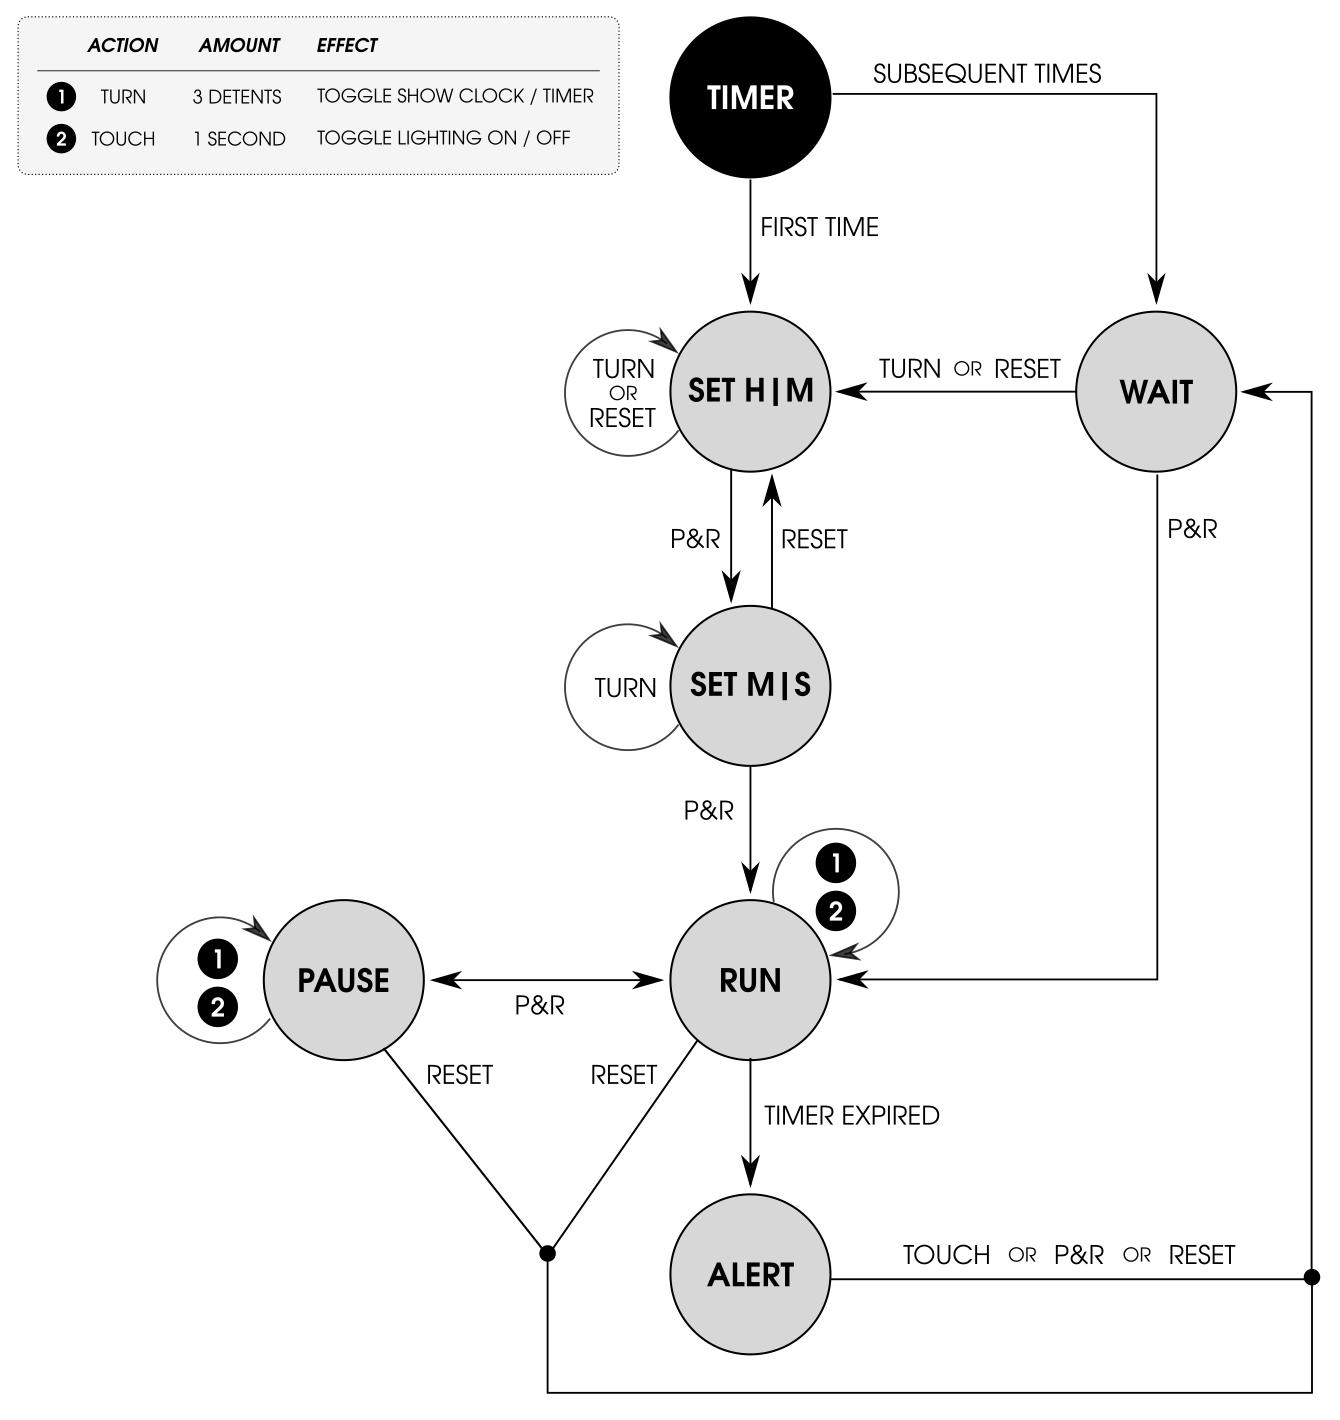
\includegraphics{images/timer_state_diagram.png}
  \caption{Timer - State Diagram}
\end{figure}


%%%%%%%%%%%%%%%%%%%%%%%%%%%%%%%%%%%%%%%%%%%%%%%%%%%%%%%%%%%%%%%%%%%%%%%%%%%%%%%%
% Secondary Modes
%%%%%%%%%%%%%%%%%%%%%%%%%%%%%%%%%%%%%%%%%%%%%%%%%%%%%%%%%%%%%%%%%%%%%%%%%%%%%%%%
\part{Secondary Modes} \label{Secondary Modes}
%%%%%%%%%%%%%%%%%%%%%%%%%%%%%%%%%%%%%%%%%%%%%%%%%%%%%%%%%%%%%%%%%%%%%%%%%%%%%%%%
% Set Clock
%%%%%%%%%%%%%%%%%%%%%%%%%%%%%%%%%%%%%%%%%%%%%%%%%%%%%%%%%%%%%%%%%%%%%%%%%%%%%%%%
\chapter{Set Clock} \label{Set Clock}
\vspace{-10ex}\mSC{syml}\vskip 8ex

%%%%%%%%%%%%%%%%%%%%%%%%%%%%%%%%%%%%%%%%%%%%%%%%%%%%%%%%%%%%%%%%%%%%%%%%%%%%%%%%
% Introduction
%%%%%%%%%%%%%%%%%%%%%%%%%%%%%%%%%%%%%%%%%%%%%%%%%%%%%%%%%%%%%%%%%%%%%%%%%%%%%%%%
\section{Introduction}

Allows setting the date and time, selecting either \num{12} or \num{24} hour
format for displaying the time and choosing whether or not the time will be
automatically updated for Daylight Saving Time.

\par\medskip

There are a few ways to get to \mSC{f} depending on which direction the \cRs{f}
is pointing and which mode the device is currently in.  The most
straightforward way is:

\begin{enumerate}
  \item \aTu{f} the \cRs{f} to the \dLe{f}.
  \item \aPH{f} the \cEs{f} until you see \symD{====} blink on the
    \cDi{f} then \aRe{f}.
\end{enumerate}

\ers{3}
\begin{table}[H]
\centering
\begin{tabu} { X[1,c,m] | X[1,c,m] | X[1,c,m] }
  \thrule
  \thbi{Position} & \thbi{Mode} & \thbi{Action} \\ \mrule

  \sMi & \multirow{2}{*}[-1mm]{\mode{s}{ANY}}
    & $\hskip -5mm$ \sMtoL \\ \dcrule{1}{1} \dcrule{3}{3}
  \sRi & & \sRtoL \\ \mdrule

  \multirow{4}{*}[-1.5mm]{\sLe} & \mSA{sym} & \sSec \\ \dcrule{2}{3}
    & \multirow{2}{*}[-1.5mm]{\mTS{sym}} & \sSec \quad \sSec \\ \dcrule{3}{3}
    & & \sTer \quad \sSec \\ \dcrule{2}{3}
    & \state{f}{ANY} & \sLtoM \quad\quad \sMtoL \quad\quad \sSec \\

  \bhrule
\end{tabu}
\caption{Set Clock - Mode}
\end{table}

\pagebreak
A few items of note:

\begin{itemize}
  \item The date and time initially loaded will be that which the clock
    currently holds.
  \item For Daylight Saving Time, the last saved setting will be loaded.
  \item After setting the time, you can change mode, 
    and the clock will be set and saved.  This allows setting the time
    without having to go through the rest of the settings.
  \item To \aReset{f} and start over, \aPH{f} the \cEs{f} until \symD{<<<<} is
    blinking on the \cDi{f}.
\end{itemize}

%%%%%%%%%%%%%%%%%%%%%%%%%%%%%%%%%%%%%%%%%%%%%%%%%%%%%%%%%%%%%%%%%%%%%%%%%%%%%%%%
% Overview
%%%%%%%%%%%%%%%%%%%%%%%%%%%%%%%%%%%%%%%%%%%%%%%%%%%%%%%%%%%%%%%%%%%%%%%%%%%%%%%%
\section{Overview}

There are a number of states \mSC{f} can be in and are explained in the next
sections.

\ers{1.5}
\begin{table}[H]
\centering
\begin{tabu} { X[1,c,m] | X[3,l,m] }
  \thrule
  \thbi{State} & \thbi{Description} \\ \mrule

  \sSCFo{sym} & Set the time format - \num{12} or \num{24} hour. \\ \drule{2}
  \sSCHo{sym} & Set the hour. \\ \drule{2}
  \sSCMi{sym} & Set the minute. \\ \drule{2}
  \sSCMo{sym} & Set the month. \\ \drule{2}
  \sSCDa{sym} & Set the day. \\ \drule{2}
  \sSCYe{sym} & Set the year. \\ \drule{2}
  \sSCDS{sym} & Set to automatically update the time for Daylight Saving Time. \\ \drule{2}
  \sSCDo{sym} & Display clock settings. \\
  \bhrule
\end{tabu}
\caption{Set Clock - States}
\end{table}

To progress through the states, you will \aTu{f} the \cEs{f} to select a value,
then \aPR{f} the \cEs{f} to save the setting and move on to the next setting.

\tabcolsep=8pt
\as{{c c c c c c c c c c c c c}}{%
\sSCFo{sym} & \sTu & \sPR & \sSCHo{sym} & \sTu & \sPR &
\sSCMi{sym} & \sTu & \sPR & $\cdots$\quad$\cdots$ & \sSCDo{sym} & \sPR & \sSCFo{sym} \\}
\tabcolsep=12pt

When all settings have been configured, the \sSCDo{f} state cycles through and
displays each one.  It will cycle repeatedly until you \aPR{f} the \cEs{f}.

\par\medskip

After setting the minute, you can short circuit the process and the clock
will be saved and set.

\tabcolsep=7pt
\ase{3}{{m{4.5in} m{0.8in} m{0.8in} m{1mm}}}{%
  \begin{tabu}{c c c c c c c c c c}
    \sSCFo{sym} & \sTu & \sPR & \sSCHo{sym} & \sTu & \sPR
      & \sSCMi{sym} & \sTu & \sPR & \sSCMo{sym}
  \end{tabu} &
  \begin{tabu}{c}
    \sSec \\ \drule{1} \sTer \\ \drule{1} $\hskip -5.5mm$ \sLtoM \\ \drule{1} \sLtoR
  \end{tabu} &
  {\ers{0.1} \begin{tabu}{c} \eSe{sym}{CLOCK} \\ \eSa{sym}{CLOCK} \end{tabu}} & \\}
\tabcolsep=12pt

%%%%%%%%%%%%%%%%%%%%%%%%%%%%%%%%%%%%%%%%%%%%%%%%%%%%%%%%%%%%%%%%%%%%%%%%%%%%%%%%
% Format
%%%%%%%%%%%%%%%%%%%%%%%%%%%%%%%%%%%%%%%%%%%%%%%%%%%%%%%%%%%%%%%%%%%%%%%%%%%%%%%%
\section[Format]{Format\footnote{ The format is set before
  the time so that the time is displayed in the format selected.}} \sSCFo{syml}

Set either \num{12} or \num{24} hour format for the time to be displayed in.

\figDT{12!H}{12 Hour Format}{24!H}{24 Hour Format}

The time can be displayed in either \num{12} or \num{24} hour format. If
\num{12} hour format is chosen, a \textit{decimal} at the \textit{lower right}
of the \cDi{f} is the \mono{PM} indicator.

\figDT{12:00}{12 AM}{12:00.}{12 PM}

To select the format, \aTu{f} the \cEs{f} then \aPR{f} to cache the setting and
move on to the next.

\as{{c c c c}}{%
\multirow{2}{*}{\sSCFo{sym}}
  & \sTu & \sPR & \multirow{2}{*}{\sSCHo{sym}} \\
& \eUp{sym}{} & \eCa{sym}{} & \\}

%%%%%%%%%%%%%%%%%%%%%%%%%%%%%%%%%%%%%%%%%%%%%%%%%%%%%%%%%%%%%%%%%%%%%%%%%%%%%%%%
% Time
%%%%%%%%%%%%%%%%%%%%%%%%%%%%%%%%%%%%%%%%%%%%%%%%%%%%%%%%%%%%%%%%%%%%%%%%%%%%%%%%
\section{Time}

Setting the time occurs on one screen of the \cDi{f} and is composed of two
states - \sSCHo{f} and \sSCMi{f}. The current setting, first \sSCHo{f}, then
\sSCMi{f}, will be \textit{blinking}.  The time will be displayed in the format
chosen in \sSCFo{f}.  A couple of examples in \num{12} and \num{24} hour format:

\begin{table}[H]
\ers{2.5}
\begin{tabu}{X[3,l,m] | X[1,c,m] | X[1,c,m]}
  \thrule
  & \thbi{12 Hour} & \thbi{24 Hour} \\ \mrule
  Five Thirty in the Morning & \sDl{!5:30} & \sDl{05:30} \\ \drule{3}
  Five Thirty (or 17:30) in the Evening & \sDl{!5:30.} & \sDl{17:30} \\
  \bhrule
\end{tabu}
\end{table}

%%%%%%%%%%%%%%%%%%%%%%%%%%%%%%%%%%%%%%%%%%%%%%%%%%%%%%%%%%%%%%%%%%%%%%%%%%%%%%%%
% Time - Hour
%%%%%%%%%%%%%%%%%%%%%%%%%%%%%%%%%%%%%%%%%%%%%%%%%%%%%%%%%%%%%%%%%%%%%%%%%%%%%%%%
\subsection{Hour} \sSCHo{syml}

Set the hour.

\par\medskip

To select the hour, \aTu{f} the \cEs{f} then \aPR{f} to cache the setting and
move on to the next.

\as{{c c c c}}{%
\multirow{2}{*}{\sSCHo{sym}}
  & \sTu & \sPR & \multirow{2}{*}{\sSCMi{sym}} \\
& \eUp{sym}{} & \eCa{sym}{} & \\}

You can turn in either direction to get to the hour you want to set.  The hour
will wrap at the \num{0} and \num{23} hour marks if the current format is
\num{24} hour.

\begin{table}[H]
\ers{1}
\centering
\begin{tabu} { c c c }
  \mrule
  \sD{00:00} & \sCC & \sD{23:00} \\
  \mrule
\end{tabu}
\quad\quad\quad\quad
\begin{tabu} { c c c }
  \mrule
  \sD{23:00} & \sCl & \sD{00:00} \\
  \mrule
\end{tabu}
\end{table}

For \num{12} hour format, the transitions between \mono{AM} and \mono{PM} when
turning clockwise and counter-clockwise from \num{12} \mono{AM} back to
\num{12} \mono{AM} are shown below.

\ase{1}{{ c c c c c c c c}}{%
\sCl & \sD{12:00} & $\cdots$ & \sD{11:00} & \sD{12:00.}
  & $\cdots$ & \sD{11:00.} & \sD{12:00} \\ \drule{8}
\sCC & \sD{12:00} & \sD{11:00.} & $\cdots$ & \sD{12:00.}
  & \sD{11:00} & $\cdots$ & \sD{12:00} \\}

%%%%%%%%%%%%%%%%%%%%%%%%%%%%%%%%%%%%%%%%%%%%%%%%%%%%%%%%%%%%%%%%%%%%%%%%%%%%%%%%
% Time - Minute
%%%%%%%%%%%%%%%%%%%%%%%%%%%%%%%%%%%%%%%%%%%%%%%%%%%%%%%%%%%%%%%%%%%%%%%%%%%%%%%%
\subsection{Minute} \sSCMi{syml}

Set the minute.

\par\medskip

To select the minute, \aTu{f} the \cEs{f} then \aPR{f} to cache the setting and
move on to the next.

\as{{c c c c}}{%
\multirow{2}{*}{\sSCMi{sym}}
  & \sTu & \sPR & \multirow{2}{*}{\sSCYe{sym}} \\
& \eUp{sym}{} & \eCa{sym}{} & \\}

\info{At this point, after caching, you can \aTu{f} the \cRs{f} or change mode
and the alarm will be set and saved.}

%%%%%%%%%%%%%%%%%%%%%%%%%%%%%%%%%%%%%%%%%%%%%%%%%%%%%%%%%%%%%%%%%%%%%%%%%%%%%%%%
% Year
%%%%%%%%%%%%%%%%%%%%%%%%%%%%%%%%%%%%%%%%%%%%%%%%%%%%%%%%%%%%%%%%%%%%%%%%%%%%%%%%
\section[Year]{Year\footnote{ The year is set before the month and day so
  that it can be determined whether or not the year is a leap year and what the
  last day of February is.}} \sSCYe{syml}

Set the year.

\par\medskip

The allowable values are \num{300} years to either side of what the last saved
year was.

\begin{table}[H]
\centering
\ers{0.1}
\begin{tabu} to 5in {X[1,c,m] X[1,c,m] X[1,c,m]}
  \sDl{1717} & \sDl{2017} & \sDl{2317} \\
  \rowfont{\scriptsize} Minimum Year & Current Year & Maximum Year
\end{tabu}
\end{table}

To select the year, \aTu{f} the \cEs{f} then \aPR{f} to cache the setting and
move on to the next.

\as{{c c c c}}{%
\multirow{2}{*}{\sSCYe{sym}}
  & \sTu & \sPR & \multirow{2}{*}{\sSCMo{sym}} \\
& \eUp{sym}{} & \eCa{sym}{} & \\}

%%%%%%%%%%%%%%%%%%%%%%%%%%%%%%%%%%%%%%%%%%%%%%%%%%%%%%%%%%%%%%%%%%%%%%%%%%%%%%%%
% Month & Day
%%%%%%%%%%%%%%%%%%%%%%%%%%%%%%%%%%%%%%%%%%%%%%%%%%%%%%%%%%%%%%%%%%%%%%%%%%%%%%%%
\section{Month \& Day}

Setting the month and day occurs on one screen of the \cDi{f} and is composed of
two states - \sSCMo{f} and \sSCDa{f}. The current setting, first \sSCMo{f}, then
\sSCDa{f}, will be \textit{blinking}.  The month and day are delimited using a
\textit{decimal}.  A couple of examples:

\figDT{!1.01}{January 1st}{12.31}{December 31st}

%%%%%%%%%%%%%%%%%%%%%%%%%%%%%%%%%%%%%%%%%%%%%%%%%%%%%%%%%%%%%%%%%%%%%%%%%%%%%%%%
% Month & Day - Month
%%%%%%%%%%%%%%%%%%%%%%%%%%%%%%%%%%%%%%%%%%%%%%%%%%%%%%%%%%%%%%%%%%%%%%%%%%%%%%%%
\subsection{Month} \sSCMo{syml}

Set the month.

\par\medskip

To select the month, \aTu{f} the \cEs{f} then \aPR{f} to cache the setting and
move on to the next.

\as{{c c c c}}{%
\multirow{2}{*}{\sSCMo{sym}}
  & \sTu & \sPR & \multirow{2}{*}{\sSCDa{sym}} \\
& \eUp{sym}{} & \eCa{sym}{} & \\}

You can turn in either direction to get to the month you want to set.  The
month will wrap at the \num{1} and \num{12} month marks.

\begin{table}[H]
\ers{1}
\centering
\begin{tabu} { c c c }
  \mrule \sD{!1.01} & \sCC & \sD{12.01} \\ \mrule
\end{tabu}
\quad\quad\quad\quad
\begin{tabu} { c c c }
  \mrule \sD{12.01} & \sCl & \sD{!1.01} \\ \mrule
\end{tabu}
\end{table}

%%%%%%%%%%%%%%%%%%%%%%%%%%%%%%%%%%%%%%%%%%%%%%%%%%%%%%%%%%%%%%%%%%%%%%%%%%%%%%%%
% Month & Day - Day
%%%%%%%%%%%%%%%%%%%%%%%%%%%%%%%%%%%%%%%%%%%%%%%%%%%%%%%%%%%%%%%%%%%%%%%%%%%%%%%%
\subsection{Day} \sSCDa{syml}

Set the day.

\par\medskip

To select the day, \aTu{f} the \cEs{f} then \aPR{f} to cache the setting and
move on to the next.

\as{{c c c c}}{%
\multirow{2}{*}{\sSCDa{sym}}
  & \sTu & \sPR & \multirow{2}{*}{\sSCDS{sym}} \\
& \eUp{sym}{} & \eCa{sym}{} & \\}

You can turn in either direction to get to the day you want to set.  The
day will wrap at \num{1} and whatever the maximum day for the month is.
For example:

\begin{table}[H]
\ers{1}
\centering
\begin{tabu} { c c c }
  \mrule \sD{10.01} & \sCC & \sD{10.31} \\ \mrule
\end{tabu}
\quad\quad\quad\quad
\begin{tabu} { c c c }
  \mrule \sD{10.31} & \sCl & \sD{10.01} \\ \mrule
\end{tabu}
\end{table}

\begin{table}[H]
\ers{1}
\centering
\begin{tabu} { c c c }
  \mrule \sD{!2.01} & \sCC & \sD{!2.28} \\ \mrule
\end{tabu}
\quad\quad\quad\quad
\begin{tabu} { c c c }
  \mrule \sD{!2.28} & \sCl & \sD{!2.01} \\ \mrule
\end{tabu}
\end{table}

%%%%%%%%%%%%%%%%%%%%%%%%%%%%%%%%%%%%%%%%%%%%%%%%%%%%%%%%%%%%%%%%%%%%%%%%%%%%%%%%
% Daylight Saving Time
%%%%%%%%%%%%%%%%%%%%%%%%%%%%%%%%%%%%%%%%%%%%%%%%%%%%%%%%%%%%%%%%%%%%%%%%%%%%%%%%
\section{Daylight Saving Time} \sSCDS{syml}

Set whether or not the clock will automatically adjust the time for Daylight
Saving Time.

\par\medskip

The \cDi{f} will show the following

\figDT{dS:!Y}{\mono{DST} Enabled}{dS:!n}{\mono{DST} Disabled}

and the letter on the \textit{right} side of the \textit{colon} will be
\textit{blinking}.  The \sDs{Y} stands for \textit{yes}, you want
the clock automatically adjusted and \sDs{n} stands for \textit{no},
you do not want it adjusted.

\par\medskip

To select the \sSCDS{f} setting, \aTu{f} the \cEs{f} then \aPR{f} to finish.
At this point, the \mCl{f} is \textit{set and saved}.

\as{{c c c c c}}{%
\multirow{2}{*}{\sSCDS{sym}}
  & \sTu & \multirow{2}{*}{\sPR} & \eSe{sym}{CLOCK}
  & \multirow{2}{*}{\sSADo{sym}} \\
& \eUp{sym}{} & & \eSa{sym}{CLOCK} & \\}

%%%%%%%%%%%%%%%%%%%%%%%%%%%%%%%%%%%%%%%%%%%%%%%%%%%%%%%%%%%%%%%%%%%%%%%%%%%%%%%%
% Done
%%%%%%%%%%%%%%%%%%%%%%%%%%%%%%%%%%%%%%%%%%%%%%%%%%%%%%%%%%%%%%%%%%%%%%%%%%%%%%%%
\pagebreak
\section{Done} \sSCDo{syml}

This state allows for review of the settings which are shown one by one on the
\cDi{f}.

\par\medskip

At this point you can start over or go to some other mode.  To start over and go
back to \sSCFo{f}, \aPR{f} the \cEs{f}.

\as{{c c c}}{\sSCDo{sym} & \sPR & \sSCFo{sym} \\}

To go to, say \mCl{f} mode, \aTu{f} the \cRs{f} to the \dMi{f}.

\ase{3}{{c c c}}{\sSCDo{sym} & \sLtoM & \mCl{sym} \\}

%%%%%%%%%%%%%%%%%%%%%%%%%%%%%%%%%%%%%%%%%%%%%%%%%%%%%%%%%%%%%%%%%%%%%%%%%%%%%%%%
% Power
%%%%%%%%%%%%%%%%%%%%%%%%%%%%%%%%%%%%%%%%%%%%%%%%%%%%%%%%%%%%%%%%%%%%%%%%%%%%%%%%
\section{Power}

The screens will turn \sOff{f} when the device is in \sPoNa{f} or \sPoSl{f}
states.

\begin{table}[H]
\ers{2}
\begin{tabu}{ X[1,c,m] | X[1,c,m] | X[1,c,m] }
  \thrule
  \thbi{Power State} & \thbi{Set Clock State} & \thbi{Screens} \\ \mrule

  \sPoNa{sym} & \multirow{2}{*}{\state{f}{ANY}}
    & \multirow{2}{*}{\sOff{sym}} \\ \dcrule{1}{1}
  \sPoSl{sym} & & \\

  \bhrule
\end{tabu}
\caption {Set Clock - Power}
\end{table}

%%%%%%%%%%%%%%%%%%%%%%%%%%%%%%%%%%%%%%%%%%%%%%%%%%%%%%%%%%%%%%%%%%%%%%%%%%%%%%%%
% Reference
%%%%%%%%%%%%%%%%%%%%%%%%%%%%%%%%%%%%%%%%%%%%%%%%%%%%%%%%%%%%%%%%%%%%%%%%%%%%%%%%
\section{Reference} \label{Set Clock - Reference}

\ers{2.5}
\begin{longtabu}{ X[2,c,m] | X[1,c,m] | X[4,c,m] | X[2,c,m] }
  \thrule
  \thbi{State} & \thbi{Action} & \thbi{Effect} & \thbi{Next} \\ \mdrule

  \multirow{2}{*}[-1.5mm]{\sSCFo{sym}}
    & \sTu & \eUp{sym}{FORMAT} & --- \\ \dcrule{2}{4}
  & \sPR & \eCa{sym}{FORMAT} \eBl{sym}{HOUR} & \sSCHo{sym} \\ \mrule

  \multirow{2}{*}[-1.5mm]{\sSCHo{sym}}
    & \sTu & \eUp{sym}{HOUR} & --- \\ \dcrule{2}{4}
  & \sPR & \eCa{sym}{HOUR} \eBl{sym}{MINUTE} & \sSCMi{sym} \\ \mrule

  \pagebreak
  \mrule

  \multirow{2}{*}[-1.5mm]{\sSCMi{sym}}
    & \sTu & \eUp{sym}{MINUTE} & --- \\ \dcrule{2}{4}
  & \sPR & \eCa{sym}{MINUTE} \eBl{sym}{YEAR} & \sSCYe{sym} \\ \mrule

  \multirow{2}{*}[-1.5mm]{\sSCYe{sym}}
    & \sTu & \eUp{sym}{YEAR} & --- \\ \dcrule{2}{4}
  & \sPR & \eCa{sym}{YEAR} \eBl{sym}{MONTH} & \sSCMo{sym} \\ \mrule

  \multirow{2}{*}[-1.5mm]{\sSCMo{sym}}
    & \sTu & \eUp{sym}{MONTH} & --- \\ \dcrule{2}{4}
  & \sPR & \eCa{sym}{MONTH} \eBl{sym}{DAY} & \sSCDa{sym} \\ \mrule

  \multirow{2}{*}[-1.5mm]{\sSCDa{sym}}
    & \sTu & \eUp{sym}{DAY} & --- \\ \dcrule{2}{4}
  & \sPR & \eCa{sym}{DAY} \eBl{sym}{DST} & \sSCDS{sym} \\ \mrule

  \multirow{2}{*}[-1.3mm]{\sSCDS{sym}}
    & \sTu & \eUp{sym}{DST} & --- \\ \dcrule{2}{4}
  & \sPR & \eSe{sym}{CLOCK} \eSa{sym}{CLOCK} \eDi{sym}{CLOCK} & \sSCDo{sym} \\ \mrule

  \sSCDo{sym} & \sPR & \eBl{sym}{FORMAT} & \sSCFo{sym} \\ \mrule

  \state{f}{ANY} & \sReset & \eRe{sym}{} \eBl{sym}{FORMAT} & \sSCFo{sym} \\ \mrule

  \multirow{4}{*}[-7mm]{\ers{0.1}\begin{tabu}{c}\sSCHo{sym}\\\sSCMi{sym}\\
      \enspace\sSCDo{sym}\thinspace\footnote{ The clock has already been
      set when \sSADo{ss}.}\end{tabu}\ers{3}}
    & \sSec & \multirow{4}{*}{\eCM{sym}} & \mSA{sym} \\ \dcrule{2}{2} \dcrule{4}{4}
    & \sTer & & \mTS{sym} \\ \dcrule{2}{2} \dcrule{4}{4}
    & $\hskip -5mm$ \sLtoM & & \mCl{sym} \\ \dcrule{2}{2} \dcrule{4}{4}
    & \sLtoR & & \mTi{sym} \\ \mrule

  \pagebreak
  \mrule

  \multirow{4}{*}[-7mm]{%
    \ers{0.1}\begin{tabu}{c}\sSCYe{sym}\\\sSCMo{sym}\\\sSCDa{sym}\\\sSCDS{sym}\end{tabu}}
    & \sSec & \multirow{4}{*}{\eSe{sym}{CLOCK} \eSa{sym}{CLOCK} \eCM{sym}}
      & \mSA{sym} \\ \dcrule{2}{2} \dcrule{4}{4}
    & \sTer & & \mTS{sym} \\ \dcrule{2}{2} \dcrule{4}{4}
    & $\hskip -5mm$ \sLtoM & & \mCl{sym} \\ \dcrule{2}{2} \dcrule{4}{4}
    & \sLtoR & & \mTi{sym} \\

  \bhrule
  \caption{Set Clock - Reference}
\end{longtabu}

%%%%%%%%%%%%%%%%%%%%%%%%%%%%%%%%%%%%%%%%%%%%%%%%%%%%%%%%%%%%%%%%%%%%%%%%%%%%%%%%
% State Diagram
%%%%%%%%%%%%%%%%%%%%%%%%%%%%%%%%%%%%%%%%%%%%%%%%%%%%%%%%%%%%%%%%%%%%%%%%%%%%%%%%
\section{State Diagram} \label{Set Clock State Diagram}

\begin{figure}[H]
\centering
  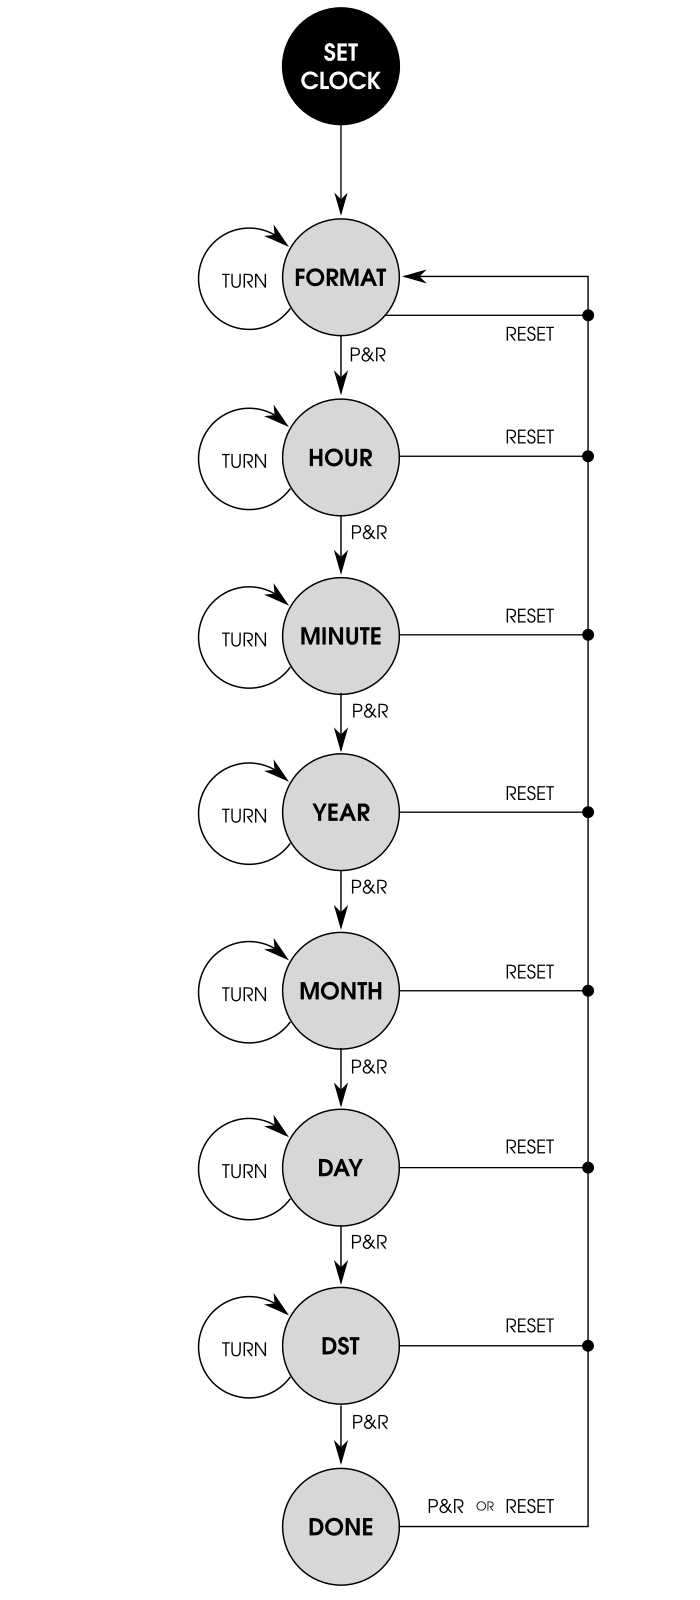
\includegraphics{images/set_clock_state_diagram.png}
\caption{Set Clock - State Diagram} 
\end{figure}

%%%%%%%%%%%%%%%%%%%%%%%%%%%%%%%%%%%%%%%%%%%%%%%%%%%%%%%%%%%%%%%%%%%%%%%%%%%%%%%%
% Power Settings
%%%%%%%%%%%%%%%%%%%%%%%%%%%%%%%%%%%%%%%%%%%%%%%%%%%%%%%%%%%%%%%%%%%%%%%%%%%%%%%%
\chapter{Power Settings} \label{Power Settings}
\vspace{-10ex}\mPS{syml}\vskip 8ex

%%%%%%%%%%%%%%%%%%%%%%%%%%%%%%%%%%%%%%%%%%%%%%%%%%%%%%%%%%%%%%%%%%%%%%%%%%%%%%%%
% Introduction
%%%%%%%%%%%%%%%%%%%%%%%%%%%%%%%%%%%%%%%%%%%%%%%%%%%%%%%%%%%%%%%%%%%%%%%%%%%%%%%%
\section{Introduction}

Allows configuring timers for putting the device into \sPoNa{f} or \sPoSl{f}
states and auto-stopping the \mAu{f}.  Also allows for configuring an amount of
time in seconds that can be used to force the device into a \sPoSl{f} state
using \aTo{f}.

\par\medskip

As a portable device that can run on the \cRB{f}, these settings can be
used to prolong the battery charge.  See \hyperref[Power]{\mPo{f}} for
information on the different power states and what they do.

\par\medskip

It is the \mSe{f} mode when the \cRs{f} is in the \dRi{f} position.

\par\medskip

There are a few ways to get to \mPS{f} depending on which direction the
\cRs{f} is pointing and which mode the device is currently in.  The most
straightforward way is:

\begin{enumerate}
  \item \aTu{f} the \cRs{f} to the \dRi{f}.
  \item \aPH{f} the \cEs{f} until \symD{====} is blinking on the \cDi{f} then
    \aRe{f}.
\end{enumerate}

\begin{table}[H]
\ers{2.0}
\centering
\begin{tabu} { X[1,c,m] | X[1,c,m] | X[1,c,m] }
  \thrule
  \thbi{Position} & \thbi{Mode} & \thbi{Action} \\ \thrule

  \sMi & \multirow{2}{*}[-1mm]{\mode{s}{ANY}}
    & $\hskip 3mm$ \sMtoR \\ \dcrule{1}{1} \dcrule{3}{3}
  \sLe & & \sLtoR \\ \mdrule

  \multirow{4}{*}[-1.5mm]{\sRi} & \mTi{sym} & \sSec \\ \dcrule{2}{3}
    & \multirow{2}{*}[-1mm]{\mSN{sym}} & \sSec \quad \sSec \\ \dcrule{3}{3}
    & & \sTer \quad \sSec \\ \dcrule{2}{3}
    & \state{f}{ANY} & \sRtoM \quad\quad \sMtoR \quad\quad \sSec \\

  \bhrule
\end{tabu}
\caption{Power Settings - Mode}
\end{table}

A few items of note:

\begin{itemize}
  \item The values initially loaded will be the last saved values.
  \item Until a setting has been saved, current \mPo{f} settings will be
    in effect.  That is, the device may \sPoNa{f} or \sPoSl{f} while in
    \mPS{f} mode, but will only do so if left idle.
  \item To \aReset{f} and start over, \aPH{f} the \cEs{f} until you see
        \symD{<<<<} blink on the \cDi{f}.
\end{itemize}

%%%%%%%%%%%%%%%%%%%%%%%%%%%%%%%%%%%%%%%%%%%%%%%%%%%%%%%%%%%%%%%%%%%%%%%%%%%%%%%%
% Overview
%%%%%%%%%%%%%%%%%%%%%%%%%%%%%%%%%%%%%%%%%%%%%%%%%%%%%%%%%%%%%%%%%%%%%%%%%%%%%%%%
\section{Overview}

There are a number of states \mTi{f} can be in and are explained in the next
sections.

\ers{1}
\begin{table}[H]
\centering
\begin{tabu} { X[1,c,m] | X[3,l,m] }
  \thrule
  \thbi{State} & \thbi{Description} \\ \mrule

  \sPSMe{sym} & Select a power setting option. \\ \drule{2}
  \sPSHM{sym} & Set the \textit{hours} or \textit{minutes}
    of the setting selected. \\ \drule{2}
  \sPSMS{sym} & Set the \textit{minutes} or \textit{seconds}
    of the setting selected. \\ \drule{2}
  \sPSSe{sym} & Set the seconds for \textit{touch} induced sleep. \\ \drule{2}
  \sPSDo{sym} & Display setting. \\
  \bhrule
\end{tabu}
\caption{Power Settings - States}
\end{table}

The \sPSMe{f} has \num{4} options to select from:

\begin{table}[H]
\ers{0.1}
\centering
\begin{tabu}{c c}
  \thi{Option} & \thi{Display} \\ \mrule
  \mPSNa{sym} & \symD{nAP!} \\
  \mPSSt{sym} & \symD{StOP} \\
  \mPSSl{sym} & \symD{SLEE.} \\
  \mPSTo{sym} & \symD{tUCH} \\
\end{tabu}
\end{table}

The general progression involves first selecting a menu option, then
setting the timer for that option.  \aTu{f} the \cEs{f} to cycle through the
menu options, \aPR{f} the \cEs{f} to select one, then proceed to set the timer
for that option.

\ase{1}{{c c l c c c c c c c c}}{%
\multirow{4}{*}{\sPSMe{sym}} & \multirow{4}{*}{\sTu}
  & \eSel{sym}{} \mPSNa{sym} & & & & & & & & \\ \dcrule{3}{3}
& & \eSel{sym}{} \mPSSt{sym} & \sPR & \sPSHM{sym} & \sTu & \sPR
  & \sPSMS{sym} & \sTu & \sPR & \sPSDo{sym} \\ \dcrule{3}{3}
& & \eSel{sym}{} \mPSSl{sym} & & & & & & & & \\ \dcrule{3}{11}
& & \eSel{sym}{} \mPSTo{sym} & \sPR & \sPSSe{sym}
  & \sTu & \sPR & \sPSDo{sym} & & & \\}

%%%%%%%%%%%%%%%%%%%%%%%%%%%%%%%%%%%%%%%%%%%%%%%%%%%%%%%%%%%%%%%%%%%%%%%%%%%%%%%%
% Menu
%%%%%%%%%%%%%%%%%%%%%%%%%%%%%%%%%%%%%%%%%%%%%%%%%%%%%%%%%%%%%%%%%%%%%%%%%%%%%%%%
\section{Menu} \sPSMe{syml}

Select a power setting to configure.

\par\medskip

The \sPSMe{f} is where you will select the power setting you want to configure a
timer for.  There are \num{4} options to select from.

\begin{table}[H]
\ers{3}
\begin{tabu}{ X[1,c,m] | X[1,c,m] }
  \thrule
  \thbi{Option} & \thbi{Display} \\ \mrule
  \mPSNa{sym} & \sDl{nAP!} \\ \drule{2}
  \mPSSt{sym} & \sDl{StOP} \\ \drule{2}
  \mPSSl{sym} & \sDl{SLEE.} \\ \drule{2}
  \mPSTo{sym} & \sDl{tUCH} \\
  \bhrule
\end{tabu}
\end{table}

\par\medskip

\mPSNa{f}, \mPSSt{f} and \mPSSl{f} can be set from \num{10} seconds
to \num{99} hours and \num{99} minutes.  Setting the timer to \symD{!0:00}
disables the setting.  If you roll over into hours a \textit{decimal} at the
\textit{bottom right} of the \cDi{f} is used to indicate that the time is in
hours and minutes or \mono{HH:MM} format.

\begin{table}[H]
\centering
\ers{0.1}
\begin{tabu}{c c c c c}
  \sDl{!0:00} & \sDl{!0:10} & \sDl{59:00} & \sDl{!1:00.} & \sDl{99:99.} \\
  \rowfont{\scriptsize} Disabled & Minimum Time & 59 Minutes & 1 Hour & Maximum Time
\end{tabu}
\end{table}

\mPSTo{f} can be set from \num{2} to \num{60} seconds.  Setting the seconds
to \symD{!!!0} disables the setting.

\begin{table}[H]
\centering
\ers{0.1}
\begin{tabu}{c c c}
  \sDl{!!!0} & \sDl{!!!2} & \sDl{!!60} \\
  \rowfont{\scriptsize} Disabled & Minimum Seconds & Maximum Seconds
\end{tabu}
\end{table}

To select an option, \aTu{f} the \cEs{f} then \aPR{f}.

\as{{c c c}}{\multirow{2}{*}{\sPSMe{sym}} & \sTu & \sPR \\
  & \eUp{sym}{MENU OPTION} & \eSel{sym}{MENU OPTION} \\}

%%%%%%%%%%%%%%%%%%%%%%%%%%%%%%%%%%%%%%%%%%%%%%%%%%%%%%%%%%%%%%%%%%%%%%%%%%%%%%%%
% Menu - Nap
%%%%%%%%%%%%%%%%%%%%%%%%%%%%%%%%%%%%%%%%%%%%%%%%%%%%%%%%%%%%%%%%%%%%%%%%%%%%%%%%
\subsection{Nap} \mPSNa{syml}

Set the amount of idle time that needs to pass before the device enters a
\sPoNa{f} power state.

\par\medskip

In addition to the timer, certain conditions must be met before the device
enters a \sPoNa{f} power state.  Refer to \hyperref[Power - Nap]{Nap} in the
\hyperref[Power]{\mPo{f}} section for more information.

\par\medskip

Set to \symD{!0:00} to disable napping.

%%%%%%%%%%%%%%%%%%%%%%%%%%%%%%%%%%%%%%%%%%%%%%%%%%%%%%%%%%%%%%%%%%%%%%%%%%%%%%%%
% Menu - Stop
%%%%%%%%%%%%%%%%%%%%%%%%%%%%%%%%%%%%%%%%%%%%%%%%%%%%%%%%%%%%%%%%%%%%%%%%%%%%%%%%
\subsection{Stop} \mPSSt{syml}

Set the amount of idle time that needs to pass before the device auto-stops the
\mAu{f}.

\par\medskip

In addition to the timer, certain conditions must be met before the device
auto-stops the \mAu{f}.  Refer to \hyperref[Power - Stop]{Audio Auto-Stop} in the
\hyperref[Power]{\mPo{f}} section for more information.

\par\medskip

Set to \symD{!0:00} to disable auto-stopping the \mAu{f}.

%%%%%%%%%%%%%%%%%%%%%%%%%%%%%%%%%%%%%%%%%%%%%%%%%%%%%%%%%%%%%%%%%%%%%%%%%%%%%%%%
% Menu - Sleep
%%%%%%%%%%%%%%%%%%%%%%%%%%%%%%%%%%%%%%%%%%%%%%%%%%%%%%%%%%%%%%%%%%%%%%%%%%%%%%%%
\subsection{Sleep} \mPSSl{syml}

Set the amount of idle time that needs to pass before the device enters a
\sPoSl{f} power state.

\par\medskip

In addition to the timer, certain conditions must be met before the device
enters a \sPoSl{f} power state.  See \hyperref[Power - Sleep]{Sleep} in the
\hyperref[Power]{\mPo{f}} section for more information.

\par\medskip

Set to \symD{!0:00} to disable sleeping.

%%%%%%%%%%%%%%%%%%%%%%%%%%%%%%%%%%%%%%%%%%%%%%%%%%%%%%%%%%%%%%%%%%%%%%%%%%%%%%%%
% Menu - Touch
%%%%%%%%%%%%%%%%%%%%%%%%%%%%%%%%%%%%%%%%%%%%%%%%%%%%%%%%%%%%%%%%%%%%%%%%%%%%%%%%
\subsection{Touch} \label{Power Settings - Touch} \mPSTo{syml}

Set the amount of time in seconds that the \cTo{f} needs to be
\textit{continuously} touched for before forcing the device into a \sPoSl{f}
power state.  See \hyperref[Power - Touch]{Touch Sleep} in the
\hyperref[Power]{\mPo{f}} section for more information.

\par\medskip

Set to \symD{!!!0} to disable touch induced sleep.

%%%%%%%%%%%%%%%%%%%%%%%%%%%%%%%%%%%%%%%%%%%%%%%%%%%%%%%%%%%%%%%%%%%%%%%%%%%%%%%%
% Timer
%%%%%%%%%%%%%%%%%%%%%%%%%%%%%%%%%%%%%%%%%%%%%%%%%%%%%%%%%%%%%%%%%%%%%%%%%%%%%%%%
\section{Timer}

Setting the timer for \mPSNa{f}, \mPSSt{f} and \mPSSl{f} menu options occurs on
one screen of the \cDi{f} and is composed of two states - \sPSHM{f} and
\sPSMS{f}. The current setting, first \sPSHM{f}, then \sPSMS{f}, will be
\textit{blinking}.

\par\medskip

The timer can be set anywhere from \num{10} seconds to \num{99} hours and
\num{99} minutes.  Set to \symD{!0:00} to disable the timer setting.

\begin{table}[H]
\centering
\ers{0.1}
\begin{tabu} to 5in {X[1,c,m] X[1,c,m] X[1,c,m]}
  \sDl{!0:00} & \sDl{!0:10} & \sDl{99:99.} \\
  \rowfont{\scriptsize} Disabled & 10 Seconds & 99 Hours \& 99 Minutes
\end{tabu}
\end{table}

To the \textit{left} of the \textit{colon} is where you set the minutes or if
more than \num{59} minutes, the hours.  As you \aTu{f} the \cEs{f} clockwise the
number will increase until it hits \num{59} minutes at which point it will
change over to hours and display a \textit{decimal} in the \textit{lower right}
of the \cDi{f}.  The decimal indicates that the time is in hours and minutes
or \mono{HH:MM}.

\figDT{59:00}{59 Minutes}{!1:00.}{1 Hour}

Like other options the numbers in the fields will wrap.  Below shows the basic
milestones as you turn in one direction or the other when in \sPSHM{f}.

\ase{1}{{ c c c c c c c c }}{%
\sCl & \sD{!0:00} & $\cdots$ & \sD{59:00} & \sD{!1:00.}
  & $\cdots$ & \sD{99:00.} & \sD{!0:00} \\ \drule{8}
\sCC & \sD{!0:00} & \sD{99:00.} & $\cdots$ & \sD{!1:00.} & \sD{59:00}
  & $\cdots$ & \sD{!0:00} \\}

If the \sPSHM{f} chosen is \num{0} then the minimum \sPSMS{f} value is
\symD{!0:10}.  The value will jump between \num{0} (disabled) and \num{10}
(minimum) when turning the \cEs{f}.

\ase{1}{{ c c c c c c }}{%
  \sCl & \sD{!0:00} & \sD{!0:10} & $\cdots$ & \sD{!0:59} & \sD{!0:00} \\ \drule{8}
  \sCC & \sD{!0:00} & \sD{!0:59} & $\cdots$ & \sD{!0:10} & \sD{!0:00} \\}

%%%%%%%%%%%%%%%%%%%%%%%%%%%%%%%%%%%%%%%%%%%%%%%%%%%%%%%%%%%%%%%%%%%%%%%%%%%%%%%%
% Timer - H|M
%%%%%%%%%%%%%%%%%%%%%%%%%%%%%%%%%%%%%%%%%%%%%%%%%%%%%%%%%%%%%%%%%%%%%%%%%%%%%%%%
\subsection{Hours or Minutes} \sPSHM{syml}

Set the timer hours or minutes.

\par\medskip

To select the \sPSHM{f}, \aTu{f} the \cEs{f} then \aPR{f} to cache the setting
and move on to \sPSMS{f}.

\as{{c c c c}}{%
\multirow{2}{*}{\sPSHM{sym}}
  & \sTu & \sPR & \multirow{2}{*}{\sPSMS{sym}} \\
& \eUp{sym}{} & \eCa{sym}{} & \\}

%%%%%%%%%%%%%%%%%%%%%%%%%%%%%%%%%%%%%%%%%%%%%%%%%%%%%%%%%%%%%%%%%%%%%%%%%%%%%%%%
% Timer - M|S
%%%%%%%%%%%%%%%%%%%%%%%%%%%%%%%%%%%%%%%%%%%%%%%%%%%%%%%%%%%%%%%%%%%%%%%%%%%%%%%%
\subsection{Minutes or Seconds} \sPSMS{syml}

Set the timer minutes or seconds.

\par\medskip

To select the \sPSMS{f}, \aTu{f} the \cEs{f} then \aPR{f} to finish.

\as{{c c c c c}}{%
\multirow{2}{*}{\sPSMS{sym}}
  & \sTu & \multirow{2}{*}{\sPR} & \eSa{sym}{TIMER}
  & \multirow{2}{*}{\sSADo{sym}} \\
& \eUp{sym}{} & & \eStart{sym}{TIMER} & \\}

%%%%%%%%%%%%%%%%%%%%%%%%%%%%%%%%%%%%%%%%%%%%%%%%%%%%%%%%%%%%%%%%%%%%%%%%%%%%%%%%
% Seconds
%%%%%%%%%%%%%%%%%%%%%%%%%%%%%%%%%%%%%%%%%%%%%%%%%%%%%%%%%%%%%%%%%%%%%%%%%%%%%%%%
\section{Seconds} \sPSSe{syml}

Set the number of seconds required for touch induced sleep.

\par\medskip

This state only applies to the \mPSTo{f} menu option.  The minimum time that can
be set is \num{2} seconds and the maximum is \num{60} seconds.  Set to
\symD{!!!0} to disable the setting.

\begin{table}[H]
\centering
\ers{0.1}
\begin{tabu} to 5in {X[1,c,m] X[1,c,m] X[1,c,m]}
  \sDl{!!!0} & \sDl{!!!2} & \sDl{!!60} \\
  \rowfont{\scriptsize} Disabled & 2 Seconds & 60 Seconds
\end{tabu}
\end{table}

To select the seconds, \aTu{f} the \cEs{f} then \aPR{f} to finish.

\as{{c c c c c}}{%
\multirow{2}{*}{\sPSSe{sym}}
  & \sTu & \multirow{2}{*}{\sPR} & \multirow{2}{*}{\eSa{sym}{TIMER}}
  & \multirow{2}{*}{\sPSDo{sym}} \\
& \eUp{sym}{} & & & \\}

%%%%%%%%%%%%%%%%%%%%%%%%%%%%%%%%%%%%%%%%%%%%%%%%%%%%%%%%%%%%%%%%%%%%%%%%%%%%%%%%
% Done
%%%%%%%%%%%%%%%%%%%%%%%%%%%%%%%%%%%%%%%%%%%%%%%%%%%%%%%%%%%%%%%%%%%%%%%%%%%%%%%%
\section{Done} \sPSDo{syml}

Displays the menu selection and timer value.

\par\medskip

At this point you can start over or go to some other mode.  To start over and go
back to \sPSMe{f}, \aPR{f} the \cEs{f}.

\as{{c c c}}{\sPSDo{sym} & \sPR & \sPSMe{sym} \\}

To go to, say \mCl{f} mode, \aTu{f} the \cRs{f} to the \dMi{f}.

\ase{3}{{c c c}}{\sPSDo{sym} & \sRtoM & \mCl{sym} \\}

%%%%%%%%%%%%%%%%%%%%%%%%%%%%%%%%%%%%%%%%%%%%%%%%%%%%%%%%%%%%%%%%%%%%%%%%%%%%%%%%
% Power
%%%%%%%%%%%%%%%%%%%%%%%%%%%%%%%%%%%%%%%%%%%%%%%%%%%%%%%%%%%%%%%%%%%%%%%%%%%%%%%%
\section{Power}

The screens will turn \sOff{f} when the device is in \sPoNa{f} or \sPoSl{f}
states.\footnote{ The current power settings will be used while you are
configuring.  When \sPSDo{ss}, the new setting will take effect.}

\begin{table}[H]
\ers{2}
\centering
\begin{tabu}{ X[1,c,m] | X[1,c,m] | X[1,c,m] }
  \thrule
  \thbi{Power State} & \thbi{Power Settings State} & \thbi{Screens} \\ \mrule

  \sPoNa{sym} & \multirow{2}{*}{\state{f}{ANY}}
    & \multirow{2}{*}{\sOff{sym}} \\ \dcrule{1}{1}
  \sPoSl{sym} & & \\

  \bhrule
\end{tabu}
\caption {Power Settings - Power}
\end{table}

%%%%%%%%%%%%%%%%%%%%%%%%%%%%%%%%%%%%%%%%%%%%%%%%%%%%%%%%%%%%%%%%%%%%%%%%%%%%%%%%
% Reference
%%%%%%%%%%%%%%%%%%%%%%%%%%%%%%%%%%%%%%%%%%%%%%%%%%%%%%%%%%%%%%%%%%%%%%%%%%%%%%%%
\pagebreak
\section{Reference} \label{Power Settings - Reference}

\ers{2.0}
\begin{longtabu}{ X[2,c,m] | X[1,c,m] | X[4,c,m] | X[2,c,m] }
  \thrule
  \thbi{State} & \thbi{Action} & \thbi{Effect} & \thbi{Next} \\ \mdrule

  \multirow{3}{*}[-10mm]{\sPSMe{sym}}
    & \sTu & \eUp{sym}{MENU OPTION} & --- \\ \dcrule{2}{4}
  & \multirow{2}{*}[-1mm]{\sPR}
    & {\ers{0.1}\tabcolsep=4pt\begin{tabu}{X[1,l,m] X[1,r,m]}
      \eSel{sym}{} \mPSNa{sym} & \\
    \eSel{sym}{} \mPSSt{sym} & \eBl{sym}{H|M} \\
    \eSel{sym}{} \mPSSl{sym} & \end{tabu}} & \sPSHM{sym} \\ \dcrule{3}{4}
  & & {\ers{0.1}\tabcolsep=4pt\begin{tabu}{X[1,l,m] X[1,r,m]}
    \eSel{sym}{} \mPSTo{sym} & \eBl{sym}{SECONDS} \end{tabu}}
    & \sPSSe{sym} \\ \mrule

  \multirow{2}{*}[-1mm]{\sPSHM{sym}}
    & \sTu & \eUp{sym}{H|M} & --- \\ \dcrule{2}{4}
  & \sPR & \eCa{sym}{H|M} \eBl{sym}{M|S} & \sPSMS{sym} \\ \mrule

  \multirow{2}{*}[-1mm]{\sPSMS{sym}}
    & \sTu & \eUp{sym}{M|S} & --- \\ \dcrule{2}{4}
    & \sPR & \eSa{sym}{TIMER} \eStart{sym}{TIMER} \eDi{sym}{TIMER}
    & \sPSDo{sym} \\ \mrule

  \multirow{2}{*}[-1mm]{\sPSSe{sym}}
    & \sTu & \eUp{sym}{SECONDS} & --- \\ \dcrule{2}{4}
  & \sPR & \eSa{sym}{TIMER} \eDi{sym}{TIMER} & \sPSDo{sym} \\ \mrule

  \sPSDo{sym} & \sPR & \eBl{sym}{MENU OPTION} & \sPSMe{sym} \\ \mrule

  \multirow{5}{*}[-1.5mm]{\state{f}{ANY}}
    & \sReset & \eRe{sym}{} \eBl{sym}{MENU OPTION}
    & \sPSMe{sym} \\ \dcrule{2}{4}
  & \sSec & \multirow{4}{*}{\eCM{sym}}
    & \mTi{sym} \\ \dcrule{2}{2} \dcrule{4}{4}
  & \sTer & & \mSN{sym} \\ \dcrule{2}{2} \dcrule{4}{4}
  & $\hskip 3mm$ \sRtoM & & \mCl{sym} \\ \dcrule{2}{2} \dcrule{4}{4}
  & \sRtoL & & \mSA{sym} \\ \mrule

  \bhrule
  \caption {Power Settings - Reference\label{table:Power Settings Reference}}
\end{longtabu}

%%%%%%%%%%%%%%%%%%%%%%%%%%%%%%%%%%%%%%%%%%%%%%%%%%%%%%%%%%%%%%%%%%%%%%%%%%%%%%%%
% State Diagram
%%%%%%%%%%%%%%%%%%%%%%%%%%%%%%%%%%%%%%%%%%%%%%%%%%%%%%%%%%%%%%%%%%%%%%%%%%%%%%%%
\section{State Diagram} \label{Power Settings State Diagram}

\begin{figure}[H]
\centering
  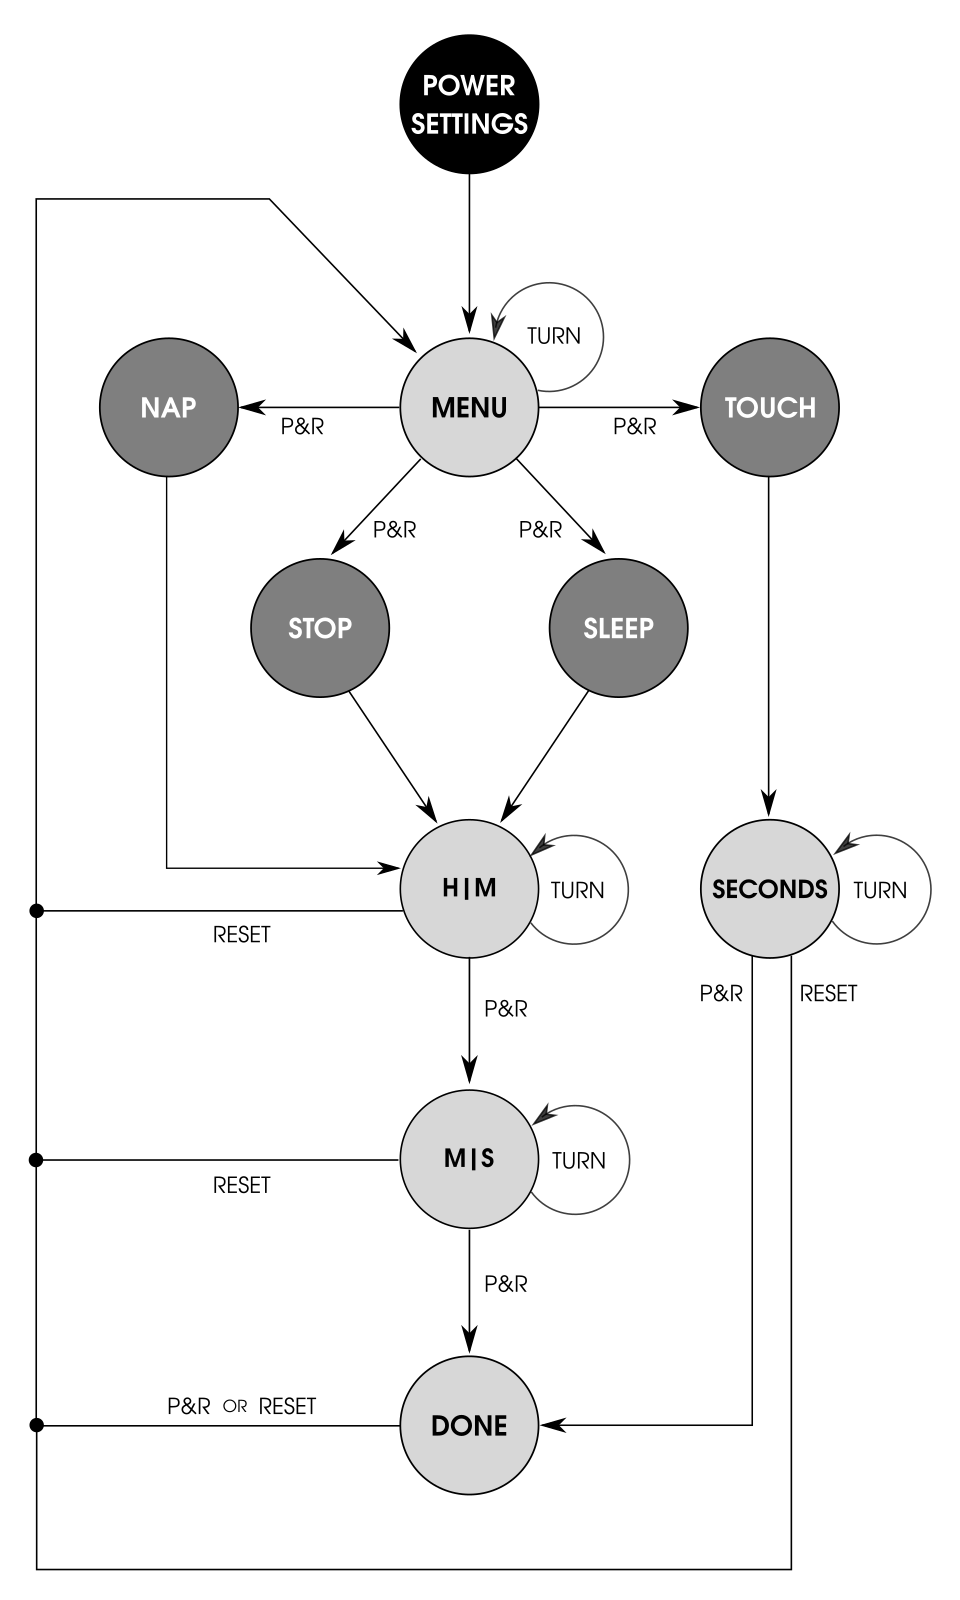
\includegraphics{images/power_settings_state_diagram.png}
  \caption{Power Settings - State Diagram}
\end{figure}


%%%%%%%%%%%%%%%%%%%%%%%%%%%%%%%%%%%%%%%%%%%%%%%%%%%%%%%%%%%%%%%%%%%%%%%%%%%%%%%%
% Tertiary Modes
%%%%%%%%%%%%%%%%%%%%%%%%%%%%%%%%%%%%%%%%%%%%%%%%%%%%%%%%%%%%%%%%%%%%%%%%%%%%%%%%
\part{Tertiary Modes} \label{Tertiary Modes}
%%%%%%%%%%%%%%%%%%%%%%%%%%%%%%%%%%%%%%%%%%%%%%%%%%%%%%%%%%%%%%%%%%%%%%%%%%%%%%%%
% Touch Settings
%%%%%%%%%%%%%%%%%%%%%%%%%%%%%%%%%%%%%%%%%%%%%%%%%%%%%%%%%%%%%%%%%%%%%%%%%%%%%%%%
\chapter{Touch Settings} \label{Touch Settings}
\vspace{-10ex}\mTS{syml}\vskip 8ex

%%%%%%%%%%%%%%%%%%%%%%%%%%%%%%%%%%%%%%%%%%%%%%%%%%%%%%%%%%%%%%%%%%%%%%%%%%%%%%%%
% Introduction
%%%%%%%%%%%%%%%%%%%%%%%%%%%%%%%%%%%%%%%%%%%%%%%%%%%%%%%%%%%%%%%%%%%%%%%%%%%%%%%%
\section{Introduction}

Allows for configuring, calibrating and testing the touch sensing capability of
the device.  It can also be disabled here.

\par\medskip

In this mode, the main goal is to come up with a number called a touch
threshold.  When a reading is taken, if its value is greater than the threshold,
a touch event is registered.  It's recommended that you first select the
\mTSCa{f} menu option and follow the instructions for that.  If you are unable
to get a consistent beep without chirping when touching during \sTSTA{f}, try
the \mTSRe{f} method, then the \mTSCo{f} method.  If nothing good comes of any
of these, you can load the \mTSDe{f} and try again or simply \mTSDi{f} touch
altogether.  Most everything that can be done using touch can be done using
other means.  There are a few exceptions:

\begin{itemize}
  \item Forcibly putting the device to sleep -
    see \hyperref[Power Settings - Touch]{Touch} in
    \hyperref[Power Settings]{\mPS{f}} and \hyperref[Power - Touch]{Touch Sleep}
    in \hyperref[Power]{\mPo{f}}.
  \item Toggling the timer lighting - see \hyperref[Timer - Lighting]{Lighting}
    in \hyperref[Timer]{\mTi{f}}.
\end{itemize}

There are a few ways to get to \mTS{f} depending on which direction the \cRs{f}
is pointing and which mode the device is currently in.  The most straightforward
way is:

\begin{enumerate}
  \item \aTu{f} the \cRs{f} to the \dLe{f}.
  \item \aPH{f} the \cEs{f} until \symD{>>>>} is blinking on the
    \cDi{f} then \aRe{f}.
\end{enumerate}

\begin{table}[H]
\ers{1}
\centering
\begin{tabu} { X[1,c,m] | X[2,c,m] | X[1,c,m] }
  \thrule
  \thbi{Position} & \thbi{Mode} & \thbi{Action} \\ \mrule

  \sMi & \multirow{2}{*}[-1.5mm]{\mode{s}{ANY}}
    & $\hskip -5mm$ \sMtoL \\ \dcrule{1}{1} \dcrule{3}{3}
  \sRi & & \sRtoL \\ \mdrule

  \multirow{2}{*}[-1.5mm]{\sLe} & \mSA{sym}
    & \multirow{2}{*}[-1.5mm]{\sTer} \\ \dcrule{2}{2}
    & \mSC{sym} & \\

  \bhrule
\end{tabu}
\caption{Touch Settings - Mode}
\end{table}

%%%%%%%%%%%%%%%%%%%%%%%%%%%%%%%%%%%%%%%%%%%%%%%%%%%%%%%%%%%%%%%%%%%%%%%%%%%%%%%%
% Capacitive Touch Sensing
%%%%%%%%%%%%%%%%%%%%%%%%%%%%%%%%%%%%%%%%%%%%%%%%%%%%%%%%%%%%%%%%%%%%%%%%%%%%%%%%
\section{Capacitive Touch Sensing}

The touch capability in this device uses
\href{https://en.wikipedia.org/wiki/Capacitive\_sensing}{Capacitive Touch Sensing}
which measures changes in capacitance of an \textit{electrode} to detect touch
events.  The figure below shows how it is modeled as a capacitor and the
corresponding parts of the device.

\begin{figure}[H]
\centering
  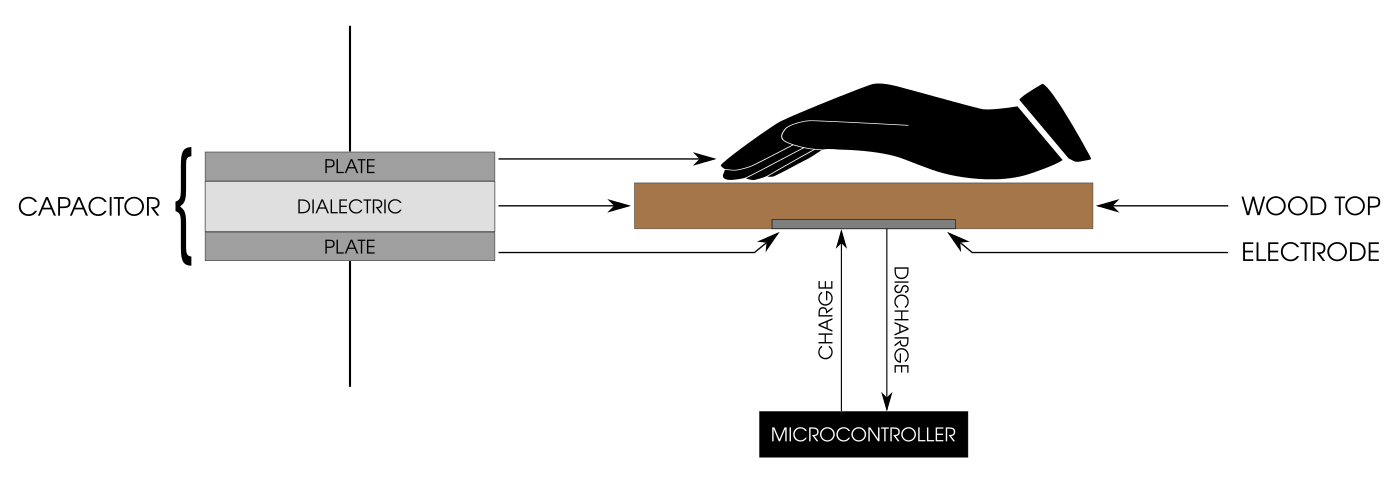
\includegraphics{images/touch_capacitive.png}
\caption{Capacitive Touch Sensing}
\end{figure}

Since humans are electrical conductors, the hand forms the other plate of the
capacitor model.  As the hand approaches and lies on \cTo{f} of the enclosure,
the capacitance, or charge capacity of the electrode will \textit{increase}.

\par\medskip

Changes in capacitance are detected by measuring the amount of time it takes to
charge and discharge the electrode.

\par\medskip

When a reading is taken, a fixed size reference capacitor is charged and
discharged using a configurable charge rate denoted as \sTSRC{f}.  At the same
time, the electrode is charged and discharged a set number of times using
another configurable charge rate denoted as \sTSEC{f}.  Since its capacitance
does \textit{not} change, the fixed size capacitor provides a \textit{reference} and will
always charge\slash discharge at the same rate.  On the other hand, the
electrode capacitance \textit{varies}, so its charge\slash discharge rate will
vary.  The number of times the electrode is charged\slash discharged or
\textit{scanned} per reading is determined by two configurable quantities
denoted as \sTSNS{f} and \sTSPS{f}.  \sTSNS{f} is a base
\textit{number of scans} and \sTSPS{f} is a \textit{prescaler} or multiplier
applied to \sTSNS{f}.  The product of the two determines the number of times the
electrode is charged\slash discharged during a reading.

\begin{figure}[H]
\centering
  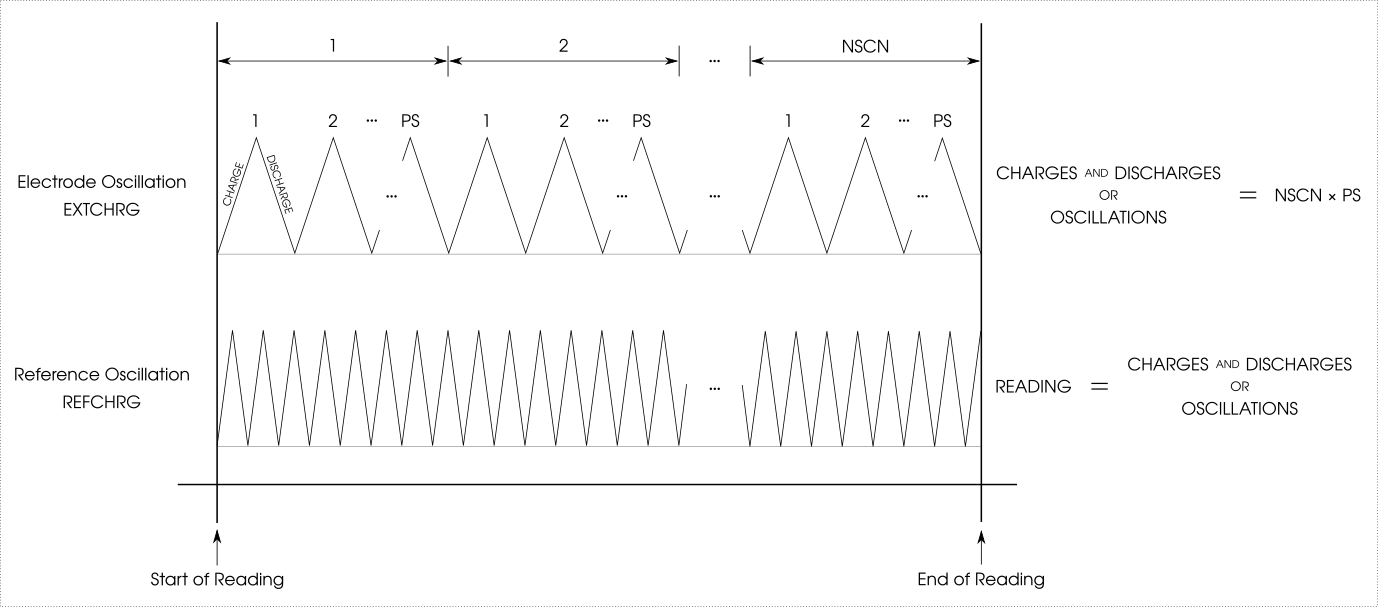
\includegraphics{images/touch_oscillation_graph.png}
\caption{Anatomy of a Touch Sensor Reading}
\end{figure}

As the hand approaches the electrode, the capacitance \textit{increases} resulting in
more time required to charge and discharge the electrode.  This increase in time
or decreased frequency results in more reference capacitor charges and
discharges per electrode charge\slash discharge resulting in a higher reading.

\par\medskip

As an analogy, consider the filling and draining of a bath tub - the larger the
tub, the longer it will take to fill it up and to drain it.  Think of the
electrode as a bath tub that increases in size when touched therefore taking
longer to fill and drain.  This increase in fill\slash drain time of the
electrode when touched means that the fixed size reference capacitor - a bath
tub that doesn't change in size - can be filled and drained more times per
electrode fill and drain.

\par\medskip

The \fontTGA{f}{READING} taken is basically the number of times it takes to fill
and drain the fixed size reference capacitor per electrode fill and drain cycle
- the cycle being defined as \sTSNS{f} $\times$ \sTSPS{f}.

\par\medskip

Below are two graphs that illustrate the capacitance difference and how it is
measured.  The first illustrates a reading taken when \textit{not touched} and
the second when \textit{touched}.  This example uses $\textrm{\sTSNS{f}} = 3$
and $\textrm{\sTSPS{f}} = 2$, so the number of electrode scans per reading is:
$\textrm{\sTSNS{f}} \times \textrm{\sTSPS{f}} = 6$.

\begin{figure}[H]
\centering
  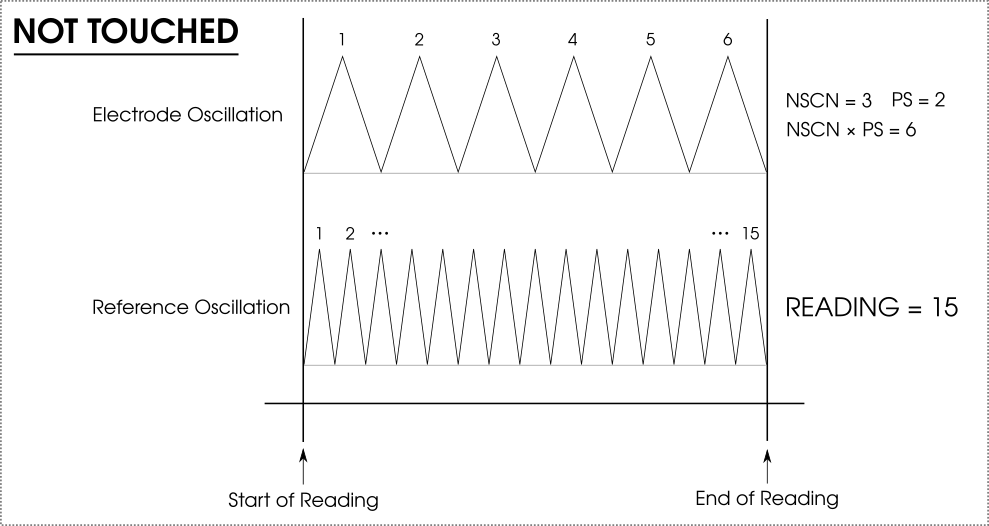
\includegraphics{images/touch_comparison_not_touched.png}
\caption{Touch Reading Comparison - Not Touched}
\end{figure}

\begin{figure}[H]
\centering
  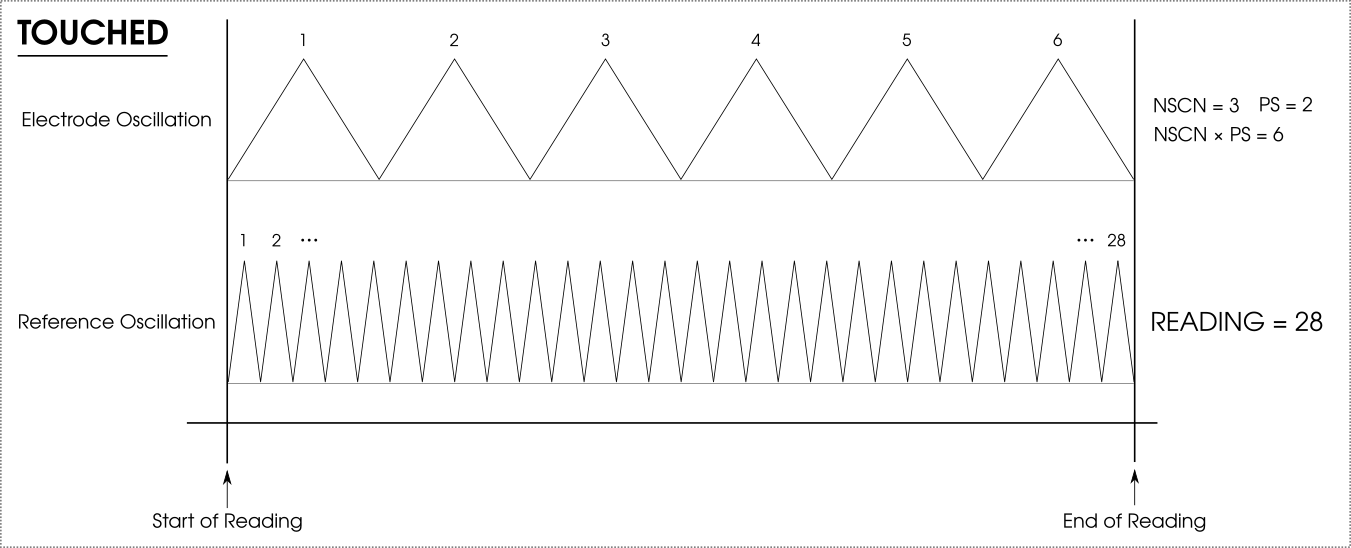
\includegraphics{images/touch_comparison_touched.png}
\caption{Touch Reading Comparison - Touched}
\end{figure}

When touched, the higher capacitance created means that it will take longer to
charge and discharge resulting in more reference oscillations per electrode scan
and therefore a higher reading.

\par\medskip

Despite the fact that a reading can be calculated, the device still has to be
told when a reading should be considered as a legitimate touch event.  As
initially mentioned, the main goal of \mTS{f} is to come up with a touch
\textit{threshold} value.  This is a value for which a touch event is registered
when the value of a reading equals or exceeds it.

\par\medskip

In the above example, if the threshold value was between \num{16} and \num{28}
inclusive, a touch event would \textit{not} have been registered in the
\fontTGA{f}{NO TOUCH} case and \textit{would} have been registered in the
\fontTGA{f}{TOUCH} case, as expected.

\par\medskip

However, if the threshold value was set to \num{15} or less, a touch event
\textit{would} have been registered in the \fontTGA{f}{NO TOUCH} case as well
as the \fontTGA{f}{TOUCH} case.  And if the threshold value was greater than
\num{28}, \textit{no} touch event would have be registered in either case.
These outcomes are unexpected and undesirable.

\par\medskip

The preceding explanation of how capacitive touch sensing works on this device is
simplified and idealized.  The reality is that readings will fluctuate.  It's
possible that readings may differ when the device is in different locations or
environmental conditions.  Additionally, when touching, readings will vary based
on how much of the hand is covering the electrode and how much force is used.
Keep this in mind during the \sTSTA{f} phase when setting the final threshold
value.  Try not to choose a value on the edge, but somewhere
\textit{above and beyond} the \textit{highest} reading when \textit{not}
touching and somewhere around an \textit{average} reading when
\textit{touching}.\footnote{ The \mTSCa{ss} procedure takes some of the guess
work out of this decision.}

%%%%%%%%%%%%%%%%%%%%%%%%%%%%%%%%%%%%%%%%%%%%%%%%%%%%%%%%%%%%%%%%%%%%%%%%%%%%%%%%
% Overview
%%%%%%%%%%%%%%%%%%%%%%%%%%%%%%%%%%%%%%%%%%%%%%%%%%%%%%%%%%%%%%%%%%%%%%%%%%%%%%%%
\section{Overview}

There are a number of states \mTS{f} can be in and are explained in the next
sections.

\ers{2}
\begin{longtabu} { X[1,c,m] | X[3,l,m] }
  \thrule
  \thbi{State} & \thbi{Description} \\ \mrule

  \sTSMe{sym} & Select a menu option. \\ \mrule
  \multicolumn{2}{c}{\mTSCa{sym}} \\ \mrule
  \sTSWB{sym} & Wait before baseline calibration run. \\ \drule{2}
  \sTSBR{sym} & Baseline calibration run. \\ \drule{2}
  \sTSWT{sym} & Wait before touch calibration run. \\ \drule{2}
  \sTSTR{sym} & Touch calibration run. \\ \mrule
  \multicolumn{2}{c}{\mTSRe{sym}} \\ \mrule
  \sTSRT{sym} & Set initial touch threshold by touching and reading value. \\ \mrule
  \multicolumn{2}{c}{\mTSCo{sym}} \\ \mrule
  \sTSNS{sym} & Configure the number of scans per reading. \\ \drule{2}
  \sTSPS{sym} & Configure the prescaler - the multiplier applied to \sTSNS{f}. \\ \drule{2}
  \sTSRC{sym} & Configure the reference charge per reading. \\ \drule{2}
  \sTSEC{sym} & Configure the external\slash electrode charge per reading. \\ \mrule
  \multicolumn{2}{c}{\mTSCa{sym} \mTSRe{sym} \mTSCo{sym}} \\ \mrule
  \sTSTA{sym} & Test and adjust touch threshold value. \\ \mrule
  \multicolumn{2}{c}{\mTSCa{sym} \mTSRe{sym} \mTSCo{sym} \mTSDe{sym}} \\ \mrule
  \sTSDo{sym} & Display settings. \\ \mrule
  \multicolumn{2}{c}{\mTSDi{sym}} \\ \mrule
  \sTSDi{sym} & Touch disabled. \\
  \bhrule
\caption{Touch Settings - States}
\end{longtabu}

%%%%%%%%%%%%%%%%%%%%%%%%%%%%%%%%%%%%%%%%%%%%%%%%%%%%%%%%%%%%%%%%%%%%%%%%%%%%%%%%
% Overview - Menu
%%%%%%%%%%%%%%%%%%%%%%%%%%%%%%%%%%%%%%%%%%%%%%%%%%%%%%%%%%%%%%%%%%%%%%%%%%%%%%%%
\sTSMe{sym} \par\medskip

The general progression through the states starts with the \sTSMe{f}.  The
\sTSMe{f} has \num{5} options to select from.

\begin{table}[H]
\ers{0.1}
\centering
\begin{tabu}{c c}
  \thi{Option} & \thi{Display} \\ \mrule
  \mTSCa{sym} & \symD{CAL.!} \\
  \mTSRe{sym} & \symD{rEAd} \\
  \mTSCo{sym} & \symD{ConF.} \\
  \mTSDe{sym} & \symD{dEF.!} \\
  \mTSDi{sym} & \symD{OFF!}
\end{tabu}
\end{table}

To select an option, \aTu{f} the \cEs{f} then \aPR{f}.

\as{{c c c c}}{\sTSMe{sym} & \sTu & \sPR & \eSel{sym}{MENU OPTION} \\}

After selecting a menu option, the path taken is dependent on the option
selected.  The paths for \mTSCa{f}, \mTSRe{f} and \mTSCo{f} all lead to
\sTSTA{f} while \mTSDe{f} goes directly to the \sTSDo{f} state and \mTSDi{f} to
the \sTSDi{f} state.

\as{{c c c}}{%
\mTSCa{sym} & & \\
\mTSRe{sym} & $\cdots$ & \sTSTA{sym} \\
\mTSCo{sym} & & \\ \drule{3}
\mTSDe{sym} & $\longrightarrow$ & \sTSDo{sym} \\ \drule{3}
\mTSDi{sym} & $\longrightarrow$ & \sTSDi{sym} \\}

%%%%%%%%%%%%%%%%%%%%%%%%%%%%%%%%%%%%%%%%%%%%%%%%%%%%%%%%%%%%%%%%%%%%%%%%%%%%%%%%
% Overview - Test & Adjust
%%%%%%%%%%%%%%%%%%%%%%%%%%%%%%%%%%%%%%%%%%%%%%%%%%%%%%%%%%%%%%%%%%%%%%%%%%%%%%%%
\sTSTA{sym} \par\medskip

This state involves tuning the final threshold value after calibrating, reading
or configuring.  The \cTo{f} of the enclosure is touched while the \cEs{f} is
turned until a solid beep from the \cBe{f} is heard.  When satisfied, \aPR{f}
the \cEs{f} to finish.

\as{{c c c c}}{%
\sTSTA{sym} & \sTo\enspace \fontTGA{f}{\&}\enspace \sTu & \sPR & \sTSDo{sym} \\}

%%%%%%%%%%%%%%%%%%%%%%%%%%%%%%%%%%%%%%%%%%%%%%%%%%%%%%%%%%%%%%%%%%%%%%%%%%%%%%%%
% Overview - Calibration
%%%%%%%%%%%%%%%%%%%%%%%%%%%%%%%%%%%%%%%%%%%%%%%%%%%%%%%%%%%%%%%%%%%%%%%%%%%%%%%%
\mTSCa{sym} \par\medskip

Set the touch threshold via a calibration process.

\par\medskip

Calibration involves \num{3} phases.  First is a \sTSBR{f}, where a number of
readings are taken \textit{without} touching the \cTo{f} of the enclosure.
After completion, the same process is done \textit{touching} the \cTo{f} of the
enclosure.  Finally, a \sTSTA{f} adjust phase is performed to tune the final
touch threshold value.

\as{{ c c c c c c c }}{%
\mono{Phase 1}
  & \sTSWB{sym} & \sNTo & \sPR & \sTSBR{sym}
    & \eCo{sym}{RUN} & \sTSWT{sym} \\ \drule{7}
\mono{Phase 2}
  & \sTSWT{sym} & \sTo & \sPR & \sTSTR{sym}
    & \eCo{sym}{RUN} & \sTSTA{sym} \\ \drule{7}
\mono{Phase 3}
  & \sTSTA{sym} & \multicolumn{3}{c}{\sTo\enspace \fontTGA{f}{\&}\enspace \sTu}
  & \sPR & \sTSDo{sym} \\}

%%%%%%%%%%%%%%%%%%%%%%%%%%%%%%%%%%%%%%%%%%%%%%%%%%%%%%%%%%%%%%%%%%%%%%%%%%%%%%%%
% Overview - Read
%%%%%%%%%%%%%%%%%%%%%%%%%%%%%%%%%%%%%%%%%%%%%%%%%%%%%%%%%%%%%%%%%%%%%%%%%%%%%%%%
\mTSRe{sym} \par\medskip

Set the touch threshold through touch readings.

\par\medskip

Reading involves \num{2} phases.  The first is simply touching the \cTo{f} of
the enclosure which will display readings when touched. Then \aPR{f} the \cEs{f}
to carry a reading value over into \sTSTA{f} where you will tune the final touch
threshold value.

\as{{ c c c c c }}{%
\mono{Phase 1}
  & \sTSRT{sym} & \sTo & \sPR & \sTSTA{sym} \\ \drule{5}
\mono{Phase 2}
  & \sTSTA{sym} & \sTo\enspace \fontTGA{f}{\&}\enspace \sTu
  & \sPR & \sTSDo{sym} \\}

%%%%%%%%%%%%%%%%%%%%%%%%%%%%%%%%%%%%%%%%%%%%%%%%%%%%%%%%%%%%%%%%%%%%%%%%%%%%%%%%
% Overview - Configuration
%%%%%%%%%%%%%%%%%%%%%%%%%%%%%%%%%%%%%%%%%%%%%%%%%%%%%%%%%%%%%%%%%%%%%%%%%%%%%%%%
\mTSCo{sym} \par\medskip

Set the touch threshold by first configuring touch sensitivity values, then
proceeding through calibration.

\par\medskip

Configuration involves \num{4} phases.  The first is setting values relevant to
touch sensitivity.  The remaining phases are the same as with the \mTSCa{f} menu
option.

\as{{ l l c c c c c }}{%
\mono{Phase 1}
  & \multicolumn{5}{c}{\sTSNS{sym} \enspace \sTu \quad \sPR \quad
  \sTSPS{sym} \enspace \sTu \quad \sPR \quad
  \sTSRC{sym} \enspace \sTu \quad \sPR \quad
  \sTSEC{sym} \enspace \sTu \quad \sPR} & \sTSWB{sym} \\ \drule{7}
\mono{Phase 2}
  & \sTSWB{sym} & \sNTo & \sPR & \sTSBR{sym} & \eCo{sym}{RUN} & \sTSWT{sym} \\ \drule{7}
\mono{Phase 3}
  & \sTSWT{sym} & \sTo & \sPR & \sTSTR{sym} & \eCo{sym}{RUN} & \sTSTA{sym} \\ \drule{7}
\mono{Phase 4}
  & \sTSTA{sym} & \multicolumn{3}{c}{\sTo\enspace \fontTGA{f}{\&}\enspace \sTu}
  & \sPR & \sTSDo{sym} \\}

%%%%%%%%%%%%%%%%%%%%%%%%%%%%%%%%%%%%%%%%%%%%%%%%%%%%%%%%%%%%%%%%%%%%%%%%%%%%%%%%
% Overview - Defaults
%%%%%%%%%%%%%%%%%%%%%%%%%%%%%%%%%%%%%%%%%%%%%%%%%%%%%%%%%%%%%%%%%%%%%%%%%%%%%%%%
\mTSDe{sym} \par\medskip

Reset the touch sensitivity and threshold values to "safe" defaults.

\as{{ c c c }}{\mTSDe{sym} & \sPR & \sTSDo{sym} \\}

%%%%%%%%%%%%%%%%%%%%%%%%%%%%%%%%%%%%%%%%%%%%%%%%%%%%%%%%%%%%%%%%%%%%%%%%%%%%%%%%
% Overview - Disable
%%%%%%%%%%%%%%%%%%%%%%%%%%%%%%%%%%%%%%%%%%%%%%%%%%%%%%%%%%%%%%%%%%%%%%%%%%%%%%%%
\mTSDi{sym} \par\medskip

Disable touch capability.

\as{{ c c c }}{\mTSDi{sym} & \sPR & \sTSDi{sym} \\}

%%%%%%%%%%%%%%%%%%%%%%%%%%%%%%%%%%%%%%%%%%%%%%%%%%%%%%%%%%%%%%%%%%%%%%%%%%%%%%%%
% Menu
%%%%%%%%%%%%%%%%%%%%%%%%%%%%%%%%%%%%%%%%%%%%%%%%%%%%%%%%%%%%%%%%%%%%%%%%%%%%%%%%
\section{Menu} \sTSMe{syml} \label{Touch - Menu}

Select one of the \num{5} menu options.

\begin{table}[H]
\ers{3}
\begin{tabu} { X[1,c,m] | X[1,c,m] | X[4,l,m] }
  \thrule
  \thbi{Option} & \thbi{Display} & \thbi{Description} \\ \mrule
  \mTSCa{sym} & \sDl{CAL.!} & Go through a calibration process followed by testing
    and adjusting to set the final touch threshold value. \\ \drule{3}
  \mTSRe{sym} & \sDl{rEAd} & Get touch readings 
    then test and adjust to set the final touch threshold value. \\ \drule{3}
  \mTSCo{sym} & \sDl{ConF.} & Configure various settings relevant to touch
    sensitivity before going through the calibration process. \\ \drule{3}
  \mTSDe{sym} & \sDl{dEF.!} & Load default touch sensitivity and
    threshold values. \\ \drule{3}
  \mTSDi{sym} & \sDl{OFF!} & Disable touch - all touch capability on the
    device will be disabled. \\
  \bhrule
\end{tabu}
\end{table}

To select a menu option, \aTu{f} the \cEs{f} then \aPR{f} when the option you
want to select is displayed.

\as{{c c c c c c}}{%
& & & \mTSCa{sym} & $\longrightarrow$ & \sTSWB{sym} \\ \dcrule{4}{6}
& & & \mTSRe{sym} & $\longrightarrow$ & \sTSRT{sym} \\ \dcrule{4}{6}
\sTSMe{sym} & & & \mTSCo{sym} & $\longrightarrow$ & \sTSNS{sym} \\ \dcrule{4}{6}
& & & \mTSDe{sym} & $\longrightarrow$ & \sTSDo{sym} \\ \dcrule{4}{6}
& \multirow{2}{*}[16.4mm]{\begin{tabu}{c} \sTu \\ \eUp{sym}{OPTION} \end{tabu}}
  & \multirow{2}{*}[16.5mm]{\begin{tabu}{c} \sPR \\ \eSel{sym}{OPTION} \end{tabu}}
  & \mTSDi{sym} & $\longrightarrow$ & \sTSDi{sym} \\}

%%%%%%%%%%%%%%%%%%%%%%%%%%%%%%%%%%%%%%%%%%%%%%%%%%%%%%%%%%%%%%%%%%%%%%%%%%%%%%%%
% Calibrate
%%%%%%%%%%%%%%%%%%%%%%%%%%%%%%%%%%%%%%%%%%%%%%%%%%%%%%%%%%%%%%%%%%%%%%%%%%%%%%%%
\pagebreak
\section{Calibrate} \label{Touch Calibration} \mTSCa{syml}

Calibration involves \num{3} phases.  First is a \sTSBR{f}, where a number of
readings are taken \textit{without} touching the \cTo{f} of the enclosure.
After completion, the same process is done \textit{touching} the \cTo{f} of the
enclosure which is the \sTSTR{f}.  Finally, a \sTSTA{f} phase is performed to
tune the final touch threshold value.

\par\medskip

For the \sTSBR{f}, do \textit{not} touch the \cTo{f} of the enclosure.  The
highest reading when not touched is used as a baseline during the \sTSTA{f}
phase for which you can not adjust below.  It is used to prevent false touch
triggering when not being touched.

\par\medskip

For the \sTSTR{f}, \textit{lightly} place your entire hand, palm down, on
\cTo{f} of the enclosure.  There is no need to press down - just let gravity
supply the force.  An average of all of the readings is taken as a touch
threshold starting point for the \sTSTA{f} phase.

%%%%%%%%%%%%%%%%%%%%%%%%%%%%%%%%%%%%%%%%%%%%%%%%%%%%%%%%%%%%%%%%%%%%%%%%%%%%%%%%
% Calibrate - Wait Baseline
%%%%%%%%%%%%%%%%%%%%%%%%%%%%%%%%%%%%%%%%%%%%%%%%%%%%%%%%%%%%%%%%%%%%%%%%%%%%%%%%
\subsection{Wait Baseline} \sTSWB{syml}

After selecting the \mTSCa{f} menu option the device will wait for you to
proceed.  The \cDi{f} will be blinking

\begin{figure}[H]
\centering
  \sDl{bASE}
\end{figure}

and the lighting area will be lit red.

\begin{enumerate}
  \item Make sure you are \textit{not} touching the \cTo{f} of the enclosure
    before proceeding.
  \item \aPR{f} the \cEs{f} to begin the calibration procedure.
\end{enumerate}

\as{{ c c c c }}{\sTSWB{sym} & \sNTo & \sPR & \sTSBR{sym} \\}

%%%%%%%%%%%%%%%%%%%%%%%%%%%%%%%%%%%%%%%%%%%%%%%%%%%%%%%%%%%%%%%%%%%%%%%%%%%%%%%%
% Calibrate - Baseline Run
%%%%%%%%%%%%%%%%%%%%%%%%%%%%%%%%%%%%%%%%%%%%%%%%%%%%%%%%%%%%%%%%%%%%%%%%%%%%%%%%
\subsection{Baseline Run} \sTSBR{syml}

The device will proceed to take \num{65535} readings.  This phase of calibration
requires no user action so remember \textit{not} to touch the device while this
is happening.  Progress can be seen by the lighting area cycling through the
colors of the rainbow

\begin{table}[H] \ers{0.1} \begin{tabu} { c }
  \cRe \cOr \cYe \cGr \cBl \cPu \cRe
\end{tabu} \end{table}

as well as the display showing a running count of the number of readings taken
in hexadecimal from \num{0} to \num{FFFF}.  Both the lighting and the count are
simply an indication of progress and are otherwise insignificant.

\as{{ c c c c }}{\sTSBR{sym} & \sNTo & \eCo{sym}{RUN} & \sTSWT{sym} \\}

%%%%%%%%%%%%%%%%%%%%%%%%%%%%%%%%%%%%%%%%%%%%%%%%%%%%%%%%%%%%%%%%%%%%%%%%%%%%%%%%
% Calibrate - Wait Touch
%%%%%%%%%%%%%%%%%%%%%%%%%%%%%%%%%%%%%%%%%%%%%%%%%%%%%%%%%%%%%%%%%%%%%%%%%%%%%%%%
\subsection{Wait Touch} \sTSWT{syml}

After the \sTSBR{f} run is complete, the display will be blinking

\begin{figure}[H]
\centering
  \sDl{tUCH}
\end{figure}

and the lighting area will be lit red.

\begin{enumerate}
  \item Make sure you that you are \textit{touching} the \cTo{f} of the
    enclosure before proceeding.  Lightly lay your entire hand, palm down,
    on \cTo{f} of the enclosure - refer to
    \hyperref[fig:Hand Coverage]{Figure \ref*{fig:Hand Coverage}} in the
    \hyperref[Operation - Touch Sensor]{\cTS{f}} section.
  \item \aPR{f} the \cEs{f} to begin the \sTSTR{f}.
\end{enumerate}

\as{{ c c c c }}{\sTSWT{sym} & \sTo & \sPR & \sTSTR{sym} \\}

%%%%%%%%%%%%%%%%%%%%%%%%%%%%%%%%%%%%%%%%%%%%%%%%%%%%%%%%%%%%%%%%%%%%%%%%%%%%%%%%
% Calibrate - Touch Run
%%%%%%%%%%%%%%%%%%%%%%%%%%%%%%%%%%%%%%%%%%%%%%%%%%%%%%%%%%%%%%%%%%%%%%%%%%%%%%%%
\subsection{Touch Run} \sTSTR{syml}

The device will again proceed to take \num{65535} readings.  Remember to keep
your hand lightly on \cTo{f} of the enclosure while this is running.  Progress
can be seen by the lighting area cycling through the colors of the rainbow

\begin{table}[H] \ers{0.1} \begin{tabu} { c }
  \cRe \cOr \cYe \cGr \cBl \cPu \cRe
\end{tabu} \end{table}

as well as the display showing a running count of the number of readings taken
in hexadecimal from \num{0} to \num{FFFF}.

\par\medskip

When done, the \cDi{f} will show a hexadecimal representation of the average
taken over all of the readings.  Hexadecimal is used since the maximum value
that is possible for a threshold, depending on configuration, can exceed
\num{9999} which is the maximum decimal value that the \cDi{f} can show.

\par\medskip

This average value will be the starting value used during
\hyperref[Test and Adjust]{\sTSTA{f}}.

\as{{ c c c c }}{\sTSTR{sym} & \sTo & \eCo{sym}{RUN} & \sTSTA{sym} \\}

%%%%%%%%%%%%%%%%%%%%%%%%%%%%%%%%%%%%%%%%%%%%%%%%%%%%%%%%%%%%%%%%%%%%%%%%%%%%%%%%
% Read
%%%%%%%%%%%%%%%%%%%%%%%%%%%%%%%%%%%%%%%%%%%%%%%%%%%%%%%%%%%%%%%%%%%%%%%%%%%%%%%%
\section{Read} \mTSRe{syml}

This is the easiest procedure for setting the touch threshold, however, it
is not as robust as \hyperref[Touch Calibration]{\mTSCa{f}} and may result in
false positive touch events, i.e., a touch event being detected when the \cTo{f}
is \textit{not} being touched.  This is because a proper baseline is not
established, making it possible to set the threshold too low.

%%%%%%%%%%%%%%%%%%%%%%%%%%%%%%%%%%%%%%%%%%%%%%%%%%%%%%%%%%%%%%%%%%%%%%%%%%%%%%%%
% Read - Touch & Read
%%%%%%%%%%%%%%%%%%%%%%%%%%%%%%%%%%%%%%%%%%%%%%%%%%%%%%%%%%%%%%%%%%%%%%%%%%%%%%%%
\subsection{Touch \& Read} \sTSRT{syml}

Obtain a threshold starting point by lightly laying your hand across the \cTo{f}
of the enclosure.

\par\medskip

After selecting the \mTSRe{f} menu option, readings from the touch sensor will
appear on the \cDi{f} and a color will light up in the \cLi{f} window.  The
values on the \cDi{f} will likely be the same or fluctuate slightly in either
direction when \textit{not} touching the \cTo{f}.  As your hand approaches and
lies flat across the \cTo{f}, the value will increase and the color in the
\cLi{f} window will change.

\par\medskip

With your hand \textit{lightly} resting on \cTo{f} of the enclosure, \aPR{f} the
\cEs{f} to carry the value over into the \hyperref[Test and Adjust]{\sTSTA{f}}
phase.

\as{{ c c c c }}{\sTSRT{sym} & \sTo & \sPR & \sTSTA{sym} \\}

%%%%%%%%%%%%%%%%%%%%%%%%%%%%%%%%%%%%%%%%%%%%%%%%%%%%%%%%%%%%%%%%%%%%%%%%%%%%%%%%
% Configure
%%%%%%%%%%%%%%%%%%%%%%%%%%%%%%%%%%%%%%%%%%%%%%%%%%%%%%%%%%%%%%%%%%%%%%%%%%%%%%%%
\section{Configure} \label{Touch Configuration} \mTSCo{syml}

Allows for configuring values related to touch sensitivity.

\par\medskip

Selecting the \mTSCo{f} option allows for setting values that affect the touch
sensitivity of the device.  The sensitivity can be described as a range of
values for which a touch event is detected.  Higher sensitivity provides a
larger range, but may lead to erroneous events.  Lower sensitivity has a smaller
range, but may require more touching force and also may not detect touch events.

\par\medskip

There are \num{4} configurable values and related states.

\begin{table}[H]
\ers{2.5}
\begin{tabu} { X[1,c,m] | X[10,l,m] }
  \thrule
  \sTSNS{sym} & \textit{Number of Scans} per reading. \\ \drule{2}
  \sTSPS{sym} & \textit{Prescale} or multiplication factor applied to
    \sTSNS{f}. \\ \drule{2}
  \sTSRC{sym} & \textit{Reference Charge} - the amount of current in
    $\mathrm{\mu A}$ (microamps) used in charging/discharging the internal
    reference capacitor. \\ \drule{2}
  \sTSEC{sym} & \textit{External Charge} - the amount of current in
    $\mathrm{\mu A}$ (microamps) used in charging/discharging the electrode. \\
  \bhrule
\end{tabu}
\end{table}

The values as they relate to touch sensitivity can basically be described with
the following equation:

\begin{equation}
Sensitivity = \ddfrac{\textrm{\sTSEC{f}}}
  {\textrm{\sTSRC{f}} \times \textrm{\sTSNS{f}} \times \textrm{\sTSPS{f}}}
\end{equation}

The \textit{smaller} the value, the \textit{more} sensitive.

\par\medskip

After the settings are configured, the calibration process must be done. Refer
to \hyperref[Touch Calibration]{\mTSCa{f}} upon completion.

%%%%%%%%%%%%%%%%%%%%%%%%%%%%%%%%%%%%%%%%%%%%%%%%%%%%%%%%%%%%%%%%%%%%%%%%%%%%%%%%
% Configure - Number of Scans
%%%%%%%%%%%%%%%%%%%%%%%%%%%%%%%%%%%%%%%%%%%%%%%%%%%%%%%%%%%%%%%%%%%%%%%%%%%%%%%%
\subsection{Number of Scans} \sTSNS{syml}

Select the number of consecutive scans per reading.

\par\medskip

The touch module takes readings at regular intervals independent of whether
or not it is being touched. When a reading is started, so is a process of
charging and discharging the electrode.  This number represents the base number
of times it will charge\slash discharge or scan the electrode before logging a
final reading.

\par\medskip

The higher the number, the more sensitive it will be which may allow for better
detection of a wider range of touching force and proximity.  However as the
number increases, so does the amount of time it takes to complete a full scan
which if too long, may result in missed touches or inconsistent behavior.

\par\medskip

\info{After you have completed configuration and enter the calibration phase,
you can get a sense of how long a reading will take by the amount of time it
takes to do each calibration run - if it seems to take too long, you may want to
run through the configuration again and lower the value.}

\par\medskip

The \cDi{f} will show the following

\figD{nS:10}{$\mathrm{10}$ Scans}

and the number on the \textit{right} side of the \textit{colon} will be
\textit{blinking}.

\par\medskip

To select the number of scans per reading, \aTu{f} the \cEs{f} then \aPR{f}
to cache the setting and move on to \sTSPS{f}.

\as{{c c c c}}{%
\multirow{2}{*}{\sTSNS{sym}}
  & \sTu & \sPR & \multirow{2}{*}{\sTSPS{sym}} \\
& \eUp{sym}{} & \eCa{sym}{} & \\}

%%%%%%%%%%%%%%%%%%%%%%%%%%%%%%%%%%%%%%%%%%%%%%%%%%%%%%%%%%%%%%%%%%%%%%%%%%%%%%%%
% Configure - Prescaler
%%%%%%%%%%%%%%%%%%%%%%%%%%%%%%%%%%%%%%%%%%%%%%%%%%%%%%%%%%%%%%%%%%%%%%%%%%%%%%%%
\subsection{Prescaler} \sTSPS{syml}

Select a value to scale the \textit{Number of Scans}.

\par\medskip

This setting scales or multiplies the value selected in \sTSNS{f} by the value
selected here.  For example, if \num{10} was selected in \sTSNS{f} and \num{4}
is selected here, the effective number of scans will be:
\texttt{10} \textbf{$\times$} \texttt{4} $=$ \num{40} Scans per Reading.

\par\medskip

There are two reasons this is a separate setting from \sTSNS{f}:

\begin{enumerate}
  \item The hardware makes this distinction and expects two distinct values.
  \item It's quicker and easier, requiring much less turning of the \cEs{f},
    to get a value between \num{1} and \num{4096} that is the product of the
    two values.
\end{enumerate}

The \cDi{f} will show the following

\figD{PS:!4}{$\mathrm{4 \times}$ Prescaler}

and the number on the \textit{right} side of the \textit{colon} will be
\textit{blinking}.

\par\medskip

To select the prescaler, \aTu{f} the \cEs{f} then \aPR{f} to cache the setting
and move on to \sTSRC{f}.

\as{{c c c c}}{%
\multirow{2}{*}{\sTSPS{sym}}
  & \sTu & \sPR & \multirow{2}{*}{\sTSRC{sym}} \\
& \eUp{sym}{} & \eCa{sym}{} & \\}

%%%%%%%%%%%%%%%%%%%%%%%%%%%%%%%%%%%%%%%%%%%%%%%%%%%%%%%%%%%%%%%%%%%%%%%%%%%%%%%%
% Configure - Reference Charge
%%%%%%%%%%%%%%%%%%%%%%%%%%%%%%%%%%%%%%%%%%%%%%%%%%%%%%%%%%%%%%%%%%%%%%%%%%%%%%%%
\subsection{Reference Charge} \sTSRC{syml}

Select the charge rate in $\mathrm{\mu A}$ for the fixed size reference
capacitor.

\par\medskip

This setting determines the charge rate in $\mathrm{\mu A}$, i.e. microamps,
used to charge the fixed size reference capacitor when taking a reading.
The higher the charge rate, the less time it will take to charge the fixed size
reference capacitor.  A higher value here will increase the sensitivity since
it will result in a higher range of readings.

\par\medskip

The \cDi{f} will show the following

\figD{rC:16}{$\mathrm{16 \mu A}$ Reference Charge}

and the number on the \textit{right} side of the \textit{colon} will be
\textit{blinking}.

\par\medskip

To select the reference charge, \aTu{f} the \cEs{f} then \aPR{f} to cache the
setting and move on to \sTSEC{f}.

\as{{c c c c}}{%
\multirow{2}{*}{\sTSRC{sym}}
  & \sTu & \sPR & \multirow{2}{*}{\sTSEC{sym}} \\
& \eUp{sym}{} & \eCa{sym}{} & \\}

%%%%%%%%%%%%%%%%%%%%%%%%%%%%%%%%%%%%%%%%%%%%%%%%%%%%%%%%%%%%%%%%%%%%%%%%%%%%%%%%
% Configure - External Charge
%%%%%%%%%%%%%%%%%%%%%%%%%%%%%%%%%%%%%%%%%%%%%%%%%%%%%%%%%%%%%%%%%%%%%%%%%%%%%%%%
\subsection{External Charge} \sTSEC{syml}

Select the charge rate in $\mathrm{\mu A}$ for the external electrode.

\par\medskip

This setting determines the charge rate in $\mathrm{\mu A}$, i.e. microamps,
used to charge the electrode when taking a reading.  It is similar to \sTSRC{f}
but applies to the electrode instead of the reference capacitor.  The higher
the charge rate, the less time it will take to charge the electrode, other
factors being equal.  A higher value here will lessen the sensitivity since it
will result in a lower range of readings.  However, because the electrode is
relatively large, it's a good idea to keep this value high and higher than the
value chosen for \sTSRC{f}.

\par\medskip

The \cDi{f} will show the following

\figD{EC:32}{$\mathrm{32 \mu A}$ External Charge}

and the number on the \textit{right} side of the \textit{colon} will be
\textit{blinking}.

\par\medskip

To select the external\slash electrode charge, \aTu{f} the \cEs{f} then \aPR{f}
to cache the setting and move on to the \hyperref[Touch Calibration]{\mTSCa{f}}
phase.

\as{{c c c c}}{%
\multirow{2}{*}{\sTSEC{sym}}
  & \sTu & \sPR & \multirow{2}{*}{\sTSWB{sym}} \\
& \eUp{sym}{} & \eCa{sym}{} & \\}

%%%%%%%%%%%%%%%%%%%%%%%%%%%%%%%%%%%%%%%%%%%%%%%%%%%%%%%%%%%%%%%%%%%%%%%%%%%%%%%%
% Defaults
%%%%%%%%%%%%%%%%%%%%%%%%%%%%%%%%%%%%%%%%%%%%%%%%%%%%%%%%%%%%%%%%%%%%%%%%%%%%%%%%
\section{Defaults} \mTSDe{syml}

Loads "safe" default touch sensitivity and threshold values.

\par\medskip

Selecting the \mTSDe{f} menu option loads touch sensitivity and threshold
values that have been tested with this device.  This doesn't mean that they are
necessarily going to just work since as mentioned, location, environmental
factors, touching force, etc. are factors that can influence readings.
However, they can provide a sane starting point if "bad" values have been set
via \mTSCo{f}.  It's recommended that after loading the \mTSDe{f} that you
follow the \hyperref[Touch Calibration]{\mTSCa{f}} procedure.

\par\medskip

To load the \mTSDe{f}, from the \hyperref[Touch - Menu]{\sTSMe{f}}, \aTu{f}
the \cEs{f} to select the option which is shown on the \cDi{f} as
\symD{dEF.!}, then \aPR{f} to finish.

\as{{ c c c c c c}}{\sTSMe{sym} & \sTu & \eSel{sym}{} \mTSDe{sym}
  & \sPR & \eLo{sym}{DEFAULTS} & \sTSDo{sym} \\}

%%%%%%%%%%%%%%%%%%%%%%%%%%%%%%%%%%%%%%%%%%%%%%%%%%%%%%%%%%%%%%%%%%%%%%%%%%%%%%%%
% Test & Adjust
%%%%%%%%%%%%%%%%%%%%%%%%%%%%%%%%%%%%%%%%%%%%%%%%%%%%%%%%%%%%%%%%%%%%%%%%%%%%%%%%
\section{Test \& Adjust} \label{Test and Adjust} \sTSTA{syml}

Test and adjust the final threshold value.

\par\medskip

A hexadecimal value will be shown on the \cDi{f} that represents a starting
point for the final touch threshold value.\footnote{ The actual value is only
important internally and isn't something you have to remember.} The \cLi{f} area
will be lit according to how that number translates to an \mono{RGB} color.  The
color is not significant and is only used to show change and as a visual
indicator of the value.

\par\medskip

This number will ultimately, after adjustment, be the threshold value used when
detecting touch events so it's important to get this the way you want it.  If
things don't seem to be working as described, try starting over, and if that
doesn't work, try doing the configuration first, before calibration.  If all
else fails, you can disable touch altogether.

\par\medskip

If it's not already beeping, with your hand still on the \cTo{f}, slowly \aTu{f}
the \cEs{f} \textit{counter-clockwise} until you hear the
\hyperref[Beeper]{\cBe{f}} sound.

\as{{ c c c }}{\sTo & \sCC & \sBe \\}

Slowly turn until you get a good consistent beep with no chirping.  Then take
your hand off to make sure it's \textit{not} beeping.  If it is, \aTu{f} the
\cEs{f} \dCl{f} until it stops and then some.

\as{{ c c c }}{\sNTo & \sCl & \sNBe \\}

How sensitive you want it is up to you, but a good point of reference is that
it should start beeping with only a light touch.  Continue this process
\textit{with} and \textit{without} \mAu{f} playing.  For some reason, the
amplifier causes a higher degree of fluctuation in readings and you don't want
it beeping when not touching in either situation.

\warning{If it's beeping at all when \textit{not} touching, with or without the
\mAu{f} playing, the device may malfunction.  For example if you've set a touch
time for forced sleep, it may constantly sleep because it thinks it's being
touched.  Or when the alarm wakes, it may immediately snooze without actually
being touched.}

To reiterate, the beeper should continuously sound when touched with your preference of
touching force.

\as{{ c c c }}{\sTo & $\longrightarrow$ & \sBe \\}

and \textit{must} be silent when not touched.

\as{{ r l r }}{\sNTo & $\longrightarrow$ & \sNBe \\}

When the above conditions are met and you are satisfied with the touch
sensitivity, to finish, \aPR{f} the \cEs{f} to save the threshold and possible
sensitivity settings set via \hyperref[Touch Configuration]{\mTSCo{f}}.

\as{{ c c c }}{\sPR & \eSa{sym}{SETTINGS} & \sTSDo{sym} \\}

%\info{It is recommended that you test with and without the \mAu{f} playing
%since the amplifier can cause a higher fluctuation of readings.}

%%%%%%%%%%%%%%%%%%%%%%%%%%%%%%%%%%%%%%%%%%%%%%%%%%%%%%%%%%%%%%%%%%%%%%%%%%%%%%%%
% Done
%%%%%%%%%%%%%%%%%%%%%%%%%%%%%%%%%%%%%%%%%%%%%%%%%%%%%%%%%%%%%%%%%%%%%%%%%%%%%%%%
\section{Done} \sTSDo{syml}

This state allows you to review the settings which are shown one by one on
the \cDi{f}.

\par\medskip

For \mTSCa{f} and \mTSRe{f}, only the touch threshold is shown.  For \mTSCo{f}
and \mTSDe{f}, the \sTSNS{f}, \sTSPS{f}, \sTSRC{f} and \sTSEC{f} are shown in
addition to the touch threshold.

\par\medskip

To return to the \sTSMe{f}, \aPR{f} the \cEs{f}.

\as{{ c c c }}{\sTSDo{sym} & \sPR & \sTSMe{sym} \\}

To go to, say \mCl{f} mode, \aTu{f} the \cRs{f} to the \dMi{f}.

\ase{3}{{ c c c}}{\sTSDo{sym} & \sLtoM & \mCl{sym} \\}

%%%%%%%%%%%%%%%%%%%%%%%%%%%%%%%%%%%%%%%%%%%%%%%%%%%%%%%%%%%%%%%%%%%%%%%%%%%%%%%%
% Disabled
%%%%%%%%%%%%%%%%%%%%%%%%%%%%%%%%%%%%%%%%%%%%%%%%%%%%%%%%%%%%%%%%%%%%%%%%%%%%%%%%
\section{Disabled} \sTSDi{syml}

Touch capability is completely disabled on the device.

\par\medskip

This state indicates that touch has been completely disabled.  Instead of the
\sTSMe{f}, the display will show

\begin{figure}[H]
\centering
  \sDl{OFF!}
\end{figure}

and will \textit{not} be blinking.  To re-enable touch, and return to the
\sTSMe{f}, \aPR{f} the \cEs{f}.

\as{{ c c c c }}{\sTSDi{sym} & \sPR & \eEn{sym}{TOUCH} & \sTSMe{sym} \\}

To disable touch, from the \hyperref[Touch - Menu]{\sTSMe{f}}, \aTu{f} the
\cEs{f} to select the \mTSDi{f} menu option, which
is shown on the \cDi{f} as \symD{OFF!} and \textit{will} be blinking, then
\aPR{f} to disable touch capability on the device.

\as{{ c c c c c c}}{\sTSMe{sym} & \sTu & \eSel{sym}{} \mTSDi{sym}
  & \sPR & \eDisable{sym}{TOUCH} & \sTSDi{sym} \\}

%%%%%%%%%%%%%%%%%%%%%%%%%%%%%%%%%%%%%%%%%%%%%%%%%%%%%%%%%%%%%%%%%%%%%%%%%%%%%%%%
% Power
%%%%%%%%%%%%%%%%%%%%%%%%%%%%%%%%%%%%%%%%%%%%%%%%%%%%%%%%%%%%%%%%%%%%%%%%%%%%%%%%
\pagebreak
\section{Power}

The screens will either \sScDi{f} or turn \sScOf{f} depending on the current
state.  If \mTS{f} is in any of the following states, the screens will
\sDim{f} for both \sPoNa{f} and \sPoSl{f} states, however, the device will
\textit{not} go to sleep - it will instead \sPoNa{f}.

\begin{itemize}
  \item \sTSBR{f}
  \item \sTSTR{f}
  \item \sTSRT{f}
  \item \sTSTA{f}
\end{itemize}

For the other \mTS{f} states, the screens will turn \sOff{f} in both \sPoNa{f}
and \sPoSl{f} power states.

\begin{table}[H]
\ers{3}
\begin{tabu}{ X[1,c,m] | X[1,c,m] | X[1,c,m] }
  \thrule
  \thbi{Power State} & \thbi{Touch Settings State} & \thbi{Screens} \\ \mrule

  \multirow{2}{*}[-1mm]{\sPoNa{sym}}
    & {\tabcolsep=4pt \ers{0.1} \begin{tabu}{c}
      \sTSBR{sym} \sTSTR{sym} \\ \sTSRT{sym} \\ \sTSTA{sym} \end{tabu}}
    & \sDim{sym} \\ \dcrule{2}{3}
  & {\tabcolsep=4pt \ers{0.1} \begin{tabu}{c}
    \sTSMe{sym} \sTSDi{sym} \sTSDo{sym} \\ \sTSWB{sym} \sTSWT{sym} \\
    \sTSNS{sym} \sTSPS{sym} \sTSRC{sym} \sTSEC{sym} \end{tabu}}
    & \sOff{sym} \\ \mrule

  \sPoSl{sym} $\rightarrow$ \sPoNa{sym}
    & {\tabcolsep=4pt \ers{0.1} \begin{tabu}{c}
      \sTSBR{sym} \sTSTR{sym} \\ \sTSRT{sym} \\ \sTSTA{sym} \end{tabu}}
    & \sDim{sym} \\ \mrule

  \sPoSl{sym} & {\tabcolsep=4pt \ers{0.1} \begin{tabu}{c}
    \sTSMe{sym} \sTSDi{sym} \sTSDo{sym} \\ \sTSWB{sym} \sTSWT{sym} \\
    \sTSNS{sym} \sTSPS{sym} \sTSRC{sym} \sTSEC{sym} \end{tabu}}
    & \sOff{sym} \\

  \bhrule
\end{tabu}
\caption {Touch Settings - Power}
\end{table}

%%%%%%%%%%%%%%%%%%%%%%%%%%%%%%%%%%%%%%%%%%%%%%%%%%%%%%%%%%%%%%%%%%%%%%%%%%%%%%%%
% Reference
%%%%%%%%%%%%%%%%%%%%%%%%%%%%%%%%%%%%%%%%%%%%%%%%%%%%%%%%%%%%%%%%%%%%%%%%%%%%%%%%
\pagebreak
\section{Reference} \label{Touch Settings - Reference}

\ers{2.5}
\begin{longtabu}{ X[2,c,m] | X[1,c,m] | X[4,c,m] | X[2,c,m] }
  \thrule
  \thbi{State} & \thbi{Action} & \thbi{Effect} & \thbi{Next} \\ \mdrule

  \multirow{6}{*}[-10mm]{\sTSMe{sym}}
    & \sTu & \eUp{sym}{MENU OPTION} & --- \\ \dcrule{2}{4}
  & &
  {\tabcolsep=4pt \begin{tabu}{X[1,l,m] X[1,r,m]} \eSel{sym}{} \mTSCa{sym}
    & \eBl{sym}{}\symD{bASE} \end{tabu}} & \sTSWB{sym} \\ \dcrule{3}{4}
  & &
  {\tabcolsep=4pt \begin{tabu}{X[1,l,m] X[1,r,m]} \eSel{sym}{} \mTSRe{sym}
    & \eDi{sym}{READING} \end{tabu}} & \sTSRT{sym} \\ \dcrule{3}{4}
  & \sPR &
  {\tabcolsep=4pt \begin{tabu}{X[1.5,l,m] X[1,r,m]} \eSel{sym}{} \mTSCo{sym}
    & \eBl{sym}{NSCN} \end{tabu}} & \sTSNS{sym} \\ \dcrule{3}{4}
  & & 
  {\tabcolsep=4pt \ers{0.1}
    \begin{tabu}{X[1,l,m] X[1,r,m]} \multirow{2}{*}{\eSel{sym}{} \mTSDe{sym}}
    & \eLo{sym}{DEFAULTS} \\ & \eDi{sym}{DEFAULTS} \end{tabu}}
    & \sTSDo{sym} \\ \dcrule{3}{4}
  & & 
  {\tabcolsep=4pt \ers{0.1}
    \begin{tabu}{X[1,l,m] X[1,r,m]} \multirow{2}{*}{\eSel{sym}{} \mTSDi{sym}}
    & \eDisable{sym}{TOUCH} \\ & \eDi{sym}{}\symD{OFF!} \end{tabu}}
    & \sTSDi{sym} \\ \mrule

  \multirow{2}{*}[-1mm]{\sTSNS{sym}}
    & \sTu & \eUp{sym}{NSCN} & --- \\ \dcrule{2}{4}
    & \sPR & \eCa{sym}{NSCN} \eBl{sym}{PS} & \sTSPS{sym} \\ \mrule

  \multirow{2}{*}[-1mm]{\sTSPS{sym}}
    & \sTu & \eUp{sym}{PS} & --- \\ \dcrule{2}{4}
    & \sPR & \eCa{sym}{PS} \eBl{sym}{REFCHRG} & \sTSRC{sym} \\ \mrule

  \multirow{2}{*}[-1mm]{\sTSRC{sym}}
    & \sTu & \eUp{sym}{REFCHRG} & --- \\ \dcrule{2}{4}
    & \sPR & \eCa{sym}{REFCHRG} \eBl{sym}{EXTCHRG} & \sTSEC{sym} \\ \mrule

  \multirow{2}{*}[-1mm]{\sTSEC{sym}}
    & \sTu & \eUp{sym}{EXTCHRG} & --- \\ \dcrule{2}{4}
    & \sPR & \eCa{sym}{EXTCHRG} \eBl{sym}{}\symD{bASE} & \sTSWB{sym} \\ \mrule

  \pagebreak \mrule

  \sTSWB{sym} & \sPR \enspace (\sNTo) & \eStart{sym}{BASELINE RUN}
    & \sTSBR{sym} \\ \mrule

  \sTSBR{sym} & \action{ss}{RUN FINISHED}
    & \eCa{sym}{BASELINE} \eBl{sym}{}\symD{tUCH} & \sTSWT{sym} \\ \mrule

  \sTSWT{sym} & \sPR \enspace ( \sTo\enspace) & \eStart{sym}{TOUCH RUN} & \sTSTR{sym} \\ \mrule

  \sTSTR{sym} & \action{ss}{RUN FINISHED} & \eCa{sym}{THRESHOLD} \eDi{sym}{THRESHOLD}
    & \sTSTA{sym} \\ \mrule

  \multirow{2}{*}[-1mm]{\sTSRT{sym}}
    & \sTo & \eDi{sym}{READING} & --- \\ \dcrule{2}{4}
    & \sPR \enspace ( \sTo\enspace)
    & \eCa{sym}{THRESHOLD} \eDi{sym}{THRESHOLD} & \sTSTA{sym} \\ \mrule

  \multirow{4}{*}[-1.5mm]{\sTSTA{sym}}
    & \sTo & \sBe\enspace $\longrightarrow$\enspace \eAc{sym}{TOUCH DETECTED}
    & --- \\ \dcrule{2}{4}
  & \sNTo & \sNBe\enspace $\longrightarrow$\enspace \eNAc{sym}{NO TOUCH DETECTED}
    & --- \\ \dcrule{2}{4}
  & \sTu & \eUp{sym}{THRESHOLD} & --- \\ \dcrule{2}{4}
  & \sPR & \eSa{sym}{SETTINGS} \eDi{sym}{SETTINGS} & \sTSDo{sym} \\ \mrule

  \multirow{2}{*}[-1mm]{\sTSDo{sym}}
    & \sPR & \multirow{2}{*}[-1mm]{\eBl{sym}{MENU OPTION}}
    & \multirow{2}{*}[-1mm]{\sTSMe{sym}} \\ \dcrule{2}{2}
    & \sReset & & \\ \mrule

  \multirow{2}{*}[-1mm]{\sTSDi{sym}}
    & \sPR & \multirow{2}{*}[-1mm]{\eEn{sym}{TOUCH} \eBl{sym}{MENU OPTION}}
    & \multirow{2}{*}[-1mm]{\sTSMe{sym}} \\ \dcrule{2}{2}
    & \sReset & & \\ \mrule

  \pagebreak \mrule

  {\tabcolsep=4pt \ers{0.1} \begin{tabu}{c}
    \mTSCa{sym} \\ \sTSWB{sym} \end{tabu}}
    & \multirow{2}{*}[-10mm]{\sReset} & \eRe{sym}{} \eBl{sym}{}\symD{CAL.!}
    & \sTSMe{sym} \\ \dcrule{1}{1} \dcrule{3}{4}

  {\tabcolsep=4pt \ers{0.1} \begin{tabu}{c}
    \mTSCa{sym} \\ \sTSBR{sym} \\ \sTSWT{sym} \\ \sTSTR{sym} \\ \sTSTA{sym} \end{tabu}}
    & & \eRe{sym}{} \eBl{sym}{}\symD{bASE} & \sTSWB{sym} \\ \mrule

  {\tabcolsep=4pt \ers{0.1} \begin{tabu}{c}
    \mTSRe{sym} \\ \sTSRT{sym} \end{tabu}}
    & \multirow{2}{*}{\sReset} & \eRe{sym}{} \eBl{sym}{}\symD{rEAd}
    & \sTSMe{sym} \\ \dcrule{1}{1} \dcrule{3}{4}

  {\tabcolsep=4pt \ers{0.1} \begin{tabu}{c}
    \mTSRe{sym} \\ \sTSTA{sym} \end{tabu}}
    & & \eRe{sym}{} \eDi{sym}{READING} & \sTSRT{sym} \\ \mrule

  {\tabcolsep=4pt \ers{0.1} \begin{tabu}{c}
    \mTSCo{sym} \\ \sTSNS{sym} \end{tabu}}
    & \multirow{2}{*}[-30mm]{\sReset} & \eRe{sym}{} \eBl{sym}{}\symD{ConF.}
    & \sTSMe{sym} \\ \dcrule{1}{1} \dcrule{3}{4}

  {\tabcolsep=4pt \ers{0.1} \begin{tabu}{c}
    \mTSCo{sym} \\ \sTSPS{sym} \\ \sTSRC{sym} \\ \sTSEC{sym} \\ \sTSWB{sym}
    \\ \sTSBR{sym} \\ \sTSWT{sym} \\ \sTSTR{sym} \\ \sTSTA{sym} \end{tabu}}
    & & \eRe{sym}{} \eBl{sym}{NSCN} & \sTSNS{sym} \\ \mrule

  \multirow{4}{*}[3mm]{\state{f}{ANY}}
    & \sSec & \multirow{4}{*}[3mm]{\eCM{sym}}
    & \multirow{2}{*}[-1mm]{\mSA{sym}} \\ \dcrule{2}{2}
  & \sTer & & \\ \dcrule{2}{2} \dcrule{4}{4}
  & $\hskip -5mm$ \sLtoM & & \mCl{sym} \\ \dcrule{2}{2} \dcrule{4}{4}
  & \sLtoR & & \mTi{sym} \\ \mrule

  \caption{Touch Settings - Reference}
\end{longtabu}

%%%%%%%%%%%%%%%%%%%%%%%%%%%%%%%%%%%%%%%%%%%%%%%%%%%%%%%%%%%%%%%%%%%%%%%%%%%%%%%%
% State Diagram
%%%%%%%%%%%%%%%%%%%%%%%%%%%%%%%%%%%%%%%%%%%%%%%%%%%%%%%%%%%%%%%%%%%%%%%%%%%%%%%%
\section{State Diagram} \label{Touch State Diagram}

\begin{figure}[H]
\centering
  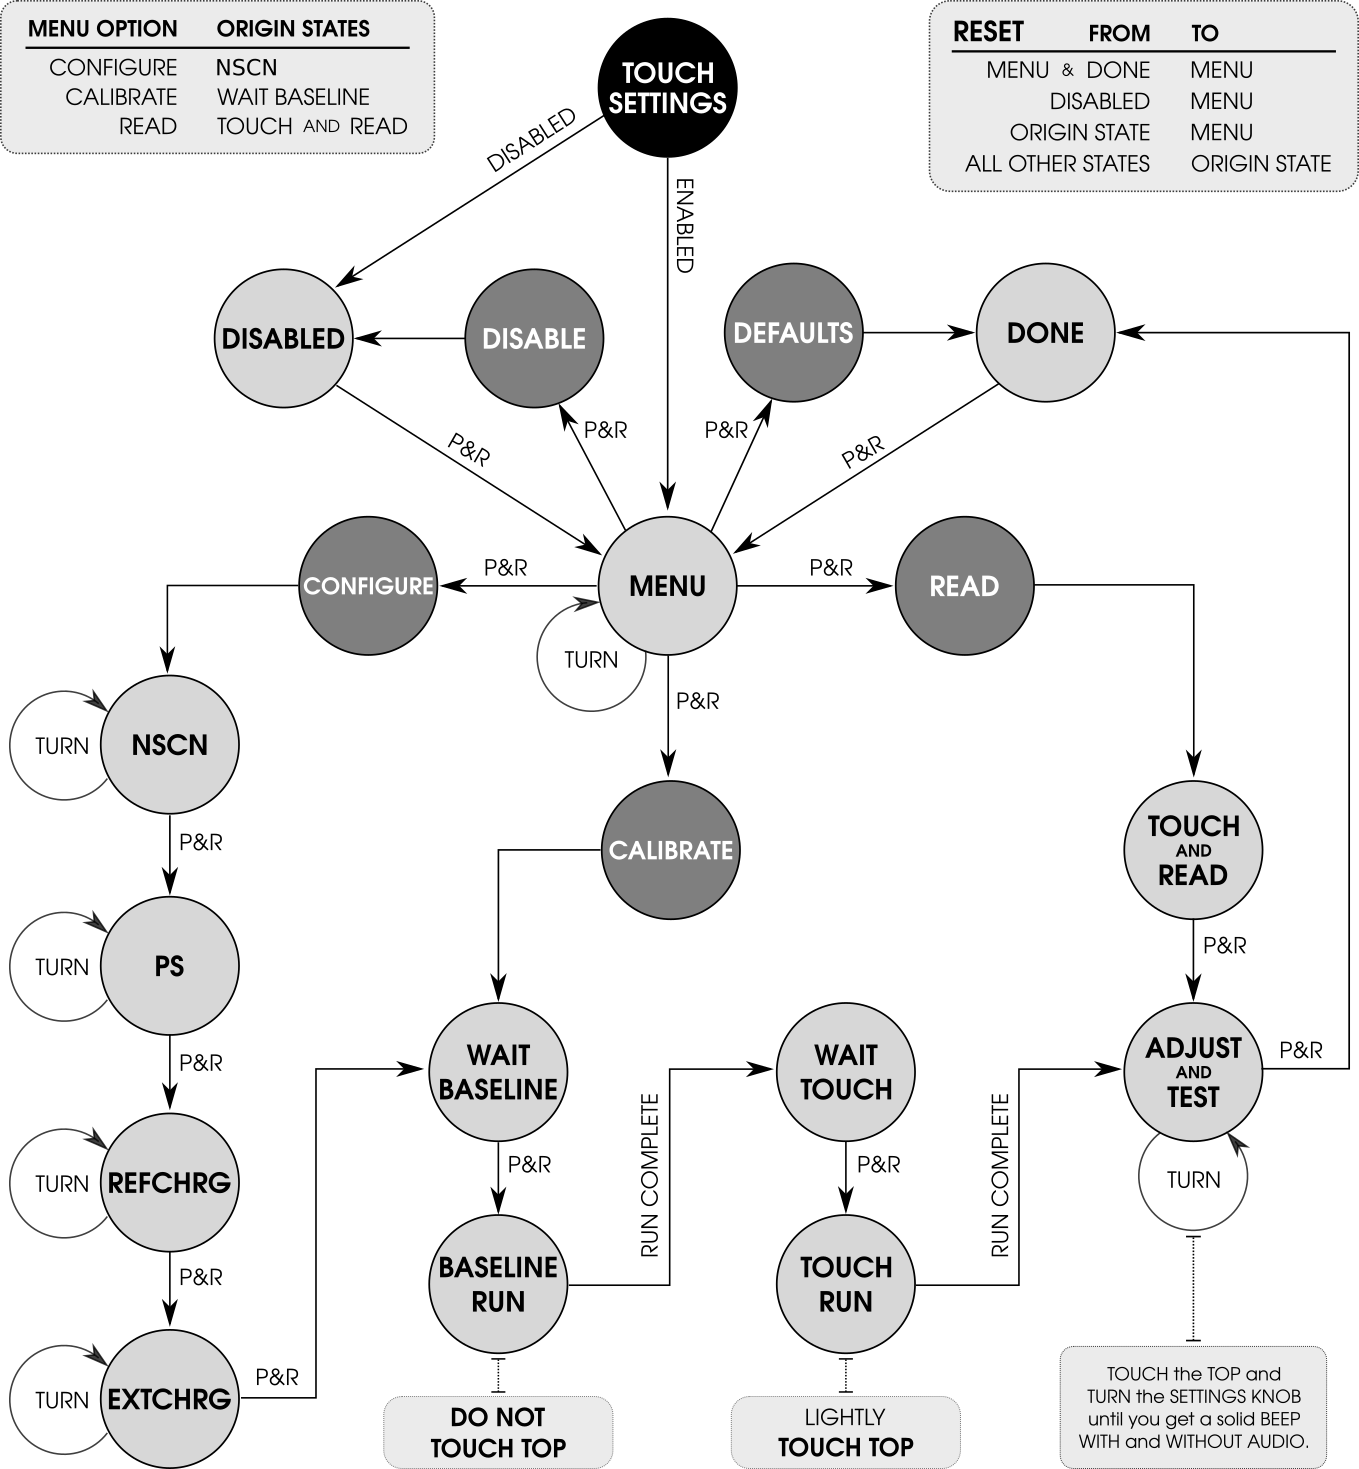
\includegraphics{images/touch_settings_state_diagram.png}
\caption{Touch Settings - State Diagram}
\end{figure}

%%%%%%%%%%%%%%%%%%%%%%%%%%%%%%%%%%%%%%%%%%%%%%%%%%%%%%%%%%%%%%%%%%%%%%%%%%%%%%%%
% Set Night Light
%%%%%%%%%%%%%%%%%%%%%%%%%%%%%%%%%%%%%%%%%%%%%%%%%%%%%%%%%%%%%%%%%%%%%%%%%%%%%%%%
\chapter{Set Night Light} \label{Set Night Light}
\vspace{-10ex}\mSN{syml}\vskip 8ex

%%%%%%%%%%%%%%%%%%%%%%%%%%%%%%%%%%%%%%%%%%%%%%%%%%%%%%%%%%%%%%%%%%%%%%%%%%%%%%%%
% Introduction
%%%%%%%%%%%%%%%%%%%%%%%%%%%%%%%%%%%%%%%%%%%%%%%%%%%%%%%%%%%%%%%%%%%%%%%%%%%%%%%%
\section{Introduction}

Allows for setting any of the \num{3} configurable night light colors using
any of \num{3} methods.

\par\medskip

The \cLi{f} is composed of \num{16}
\href{https://en.wikipedia.org/wiki/RGB\_color\_model}{RGB} LEDs.  Each LED is
composed of a Red, a Green and a Blue pixel.  The color of each LED is
determined by the blend of these pixels.

\par\medskip

There are a number of preset colors that can be chosen from.  Additionally,
the color can be customized by either selecting the individual values for the
Red, Green and Blue pixels or by selecting
\href{https://en.wikipedia.org/wiki/HSL\_and\_HSV}{HSB} values -
Hue, Saturation and Brightness.

\par\medskip

It is the \mTe{f} mode when the \cRs{f} is in the \dRi{f} position.

\par\medskip

There are a few ways to get to \mSN{f} depending on which direction the
\cRs{f} is pointing and which mode the device is currently in.  The most
straightforward way is:

\begin{enumerate}
  \item \aTu{f} the \cRs{f} to the \dRi{f}.
  \item \aPH{f} the \cEs{f} until \symD{>>>>} is blinking on the
    \cDi{f} then \aRe{f}.
\end{enumerate}

\begin{table}[H]
\ers{3}
\centering
\begin{tabu} { X[1,c,m] | X[2,c,m] | X[1,c,m] }
  \thrule
  \thbi{Position} & \thbi{Mode} & \thbi{Action} \\ \mrule

  \sMi & \multirow{2}{*}[-1mm]{\mode{s}{ANY}}
    & $\hskip 3mm$ \sMtoR \\ \dcrule{1}{1} \dcrule{3}{3}
  \sLe & & \sLtoR \\ \mdrule

  \multirow{2}{*}[-2mm]{\sRi} & \mTi{sym}
    & \multirow{2}{*}[-2mm]{\sTer} \\ \dcrule{2}{2}
  & \mPS{sym} & \\

  \bhrule
\end{tabu}
\caption{Set Night Light - Mode}
\end{table}

\pagebreak

A few items of note:

\begin{itemize}
  \item The night light number initially loaded will be the one currently
    displayed if the night light in on.
  \item When using a different method from the one used previously
    to set the color, an attempt will be made to get the settings as
    close to the color as possible.
  \item The color will be updated in real time and shown in the \cLi{f} window.
  \item When using either RGB or HSB, you will \hyperref[Double-Click]{\aDC{f}}
    the \cEs{f} to finish.  It's done this way because it is assumed that one
    will likely want to go through the process a number of times to fine tune
    the color.
  \item To \aReset{f} and start over from the top menu, \aPH{f} the \cEs{f}
    until you see \symD{<<<<} blink on the \cDi{f}.
\end{itemize}

%%%%%%%%%%%%%%%%%%%%%%%%%%%%%%%%%%%%%%%%%%%%%%%%%%%%%%%%%%%%%%%%%%%%%%%%%%%%%%%%
% Overview
%%%%%%%%%%%%%%%%%%%%%%%%%%%%%%%%%%%%%%%%%%%%%%%%%%%%%%%%%%%%%%%%%%%%%%%%%%%%%%%%
\section{Overview}

There are a number of states \mSN{f} can be in and are explained in the next
sections.

\begin{table}[H]
\ers{2}
\centering
\begin{tabu}{ X[1,c,m] | X[3,l,m] }
  \thrule
  \thbi{State} & \thbi{Description} \\ \mrule

  \sSNMN{sym} & Select one of the three night light colors
    you want to set. \\ \drule{2}
  \sSNMC{sym} & Select the method for setting the color. \\ \drule{2}
  \sSNCI{sym} & Set the color by selecting one of many
    preset colors. \\ \drule{2}
  \sSNRe{sym} & Set the Red pixel value. \\ \drule{2}
  \sSNGr{sym} & Set the Green pixel value. \\ \drule{2}
  \sSNBl{sym} & Set the Blue pixel value. \\ \drule{2}
  \sSNHu{sym} & Set a Hue value. \\ \drule{2}
  \sSNSa{sym} & Set a Saturation value. \\ \drule{2}
  \sSNBr{sym} & Set a Brightness value. \\ \drule{2}
  \sSNDo{sym} & Display settings values. \\
  \bhrule
\end{tabu}
\caption{Set Night Light - States}
\end{table}

To progress through the states, you will first \aTu{f} the \cEs{f} to select
one of the \num{3} configurable night light colors, \mSNOn{f}, \mSNTw{f} or
\mSNTh{f}, then \aPR{f} the \cEs{f}.

\ase{1}{{ c c c c c }}{%
& & \eSel{sym}{} \mSNOn{sym} & & \\ \dcrule{3}{3}
\sSNMN{sym} & \sTu & \eSel{sym}{} \mSNTw{sym} & \sPR & \sSNMC{sym} \\ \dcrule{3}{3}
& & \eSel{sym}{} \mSNTh{sym} & & \\}

The \sSNMC{f} has three options for setting the color.

\begin{table}[H]
\ers{0.1}
\centering
\begin{tabu} { c c }
  \thi{Option} & \thi{Display} \\ \mrule
  \mSNCo{sym} & \symD{CoLr} \\
  \mSNRGB{sym} & \symD{rgb!} \\
  \mSNHSB{sym} & \symD{HSb!} \\
\end{tabu}
\end{table}

\aTu{f} the \cEs{f} to select the method for setting the color of the chosen
night light then \aPR{f}.

\ase{1}{{ c c c c c }}{%
& & \eSel{sym}{} \mSNCo{sym} & & \sSNCI{sym} \\ \dcrule{3}{3} \dcrule{5}{5}
\sSNMC{sym} & \sTu & \eSel{sym}{} \mSNRGB{sym}
  & \sPR & \sSNRe{sym} \\ \dcrule{3}{3} \dcrule{5}{5}
& & \eSel{sym}{} \mSNHSB{sym} & & \sSNHu{sym} \\}

%%%%%%%%%%%%%%%%%%%%%%%%%%%%%%%%%%%%%%%%%%%%%%%%%%%%%%%%%%%%%%%%%%%%%%%%%%%%%%%%
% Overview - Preset
%%%%%%%%%%%%%%%%%%%%%%%%%%%%%%%%%%%%%%%%%%%%%%%%%%%%%%%%%%%%%%%%%%%%%%%%%%%%%%%%
\mSNCo{sym} \par\medskip

Select a preset color.

\par\medskip

This menu option is probably the easiest to use for setting the color.  There
are over \num{100} colors to choose from.  There is one state - \sSNCI{f} - when
taking this path before finishing.

\as{{ c c c c }}{ \sSNCI{sym} & \sTu & \sPR & \sSNDo{sym} \\}

%%%%%%%%%%%%%%%%%%%%%%%%%%%%%%%%%%%%%%%%%%%%%%%%%%%%%%%%%%%%%%%%%%%%%%%%%%%%%%%%
% Overview - RGB
%%%%%%%%%%%%%%%%%%%%%%%%%%%%%%%%%%%%%%%%%%%%%%%%%%%%%%%%%%%%%%%%%%%%%%%%%%%%%%%%
\mSNRGB{sym} \par\medskip

Create a color by selecting individual \sSNRe{f}, \sSNGr{f} and \sSNBl{f} pixel
values.

\par\medskip

This method allows you to select values for the individual \sSNRe{f}, \sSNGr{f}
and \sSNBl{f} pixels of the LEDs.

\ase{1}{{ c c c c c c c c c c }}{%
  \multirow{2}{*}{\sSNRe{sym}}
  & \multirow{2}{*}{\sTu}
  & \multirow{2}{*}{\sPR}
  & \multirow{2}{*}{\sSNGr{sym}}
  & \multirow{2}{*}{\sTu}
  & \multirow{2}{*}{\sPR}
  & \multirow{2}{*}{\sSNBl{sym}}
  & \multirow{2}{*}{\sTu} & \sPR & \sSNRe{sym} \\ \dcrule{9}{10}
& & & & & & & & \sDC & \sSNDo{sym} \\}

\pagebreak
At any time you can \aDC{f} to finish.

\ase{1}{{ c c c c c c c c c c }}{%
& & \sDC & \sSNDo{sym} \\ \dcrule{3}{7}
\sSNRe{sym} & \sTu
  & \multirow{2}{*}{\sPR}
  & \multirow{2}{*}{\sSNGr{sym}}
  & \multirow{2}{*}{\sTu} & \sDC & \sSNDo{sym} \\ \dcrule{6}{10}
& & & & & \sPR & \sSNBl{sym} & \sTu & \sDC & \sSNDo{sym} \\}

%%%%%%%%%%%%%%%%%%%%%%%%%%%%%%%%%%%%%%%%%%%%%%%%%%%%%%%%%%%%%%%%%%%%%%%%%%%%%%%%
% Overview - HSB
%%%%%%%%%%%%%%%%%%%%%%%%%%%%%%%%%%%%%%%%%%%%%%%%%%%%%%%%%%%%%%%%%%%%%%%%%%%%%%%%
\mSNHSB{sym} \par\medskip

Create a color by selecting \sSNHu{f}, \sSNSa{f} and \sSNBr{f} values.

\par\medskip

This method allows you to set the night light color by individually selecting
\sSNHu{f}, \sSNSa{f} and \sSNBr{f} values.

\ase{1}{{ c c c c c c c c c c }}{%
  \multirow{2}{*}{\sSNHu{sym}}
  & \multirow{2}{*}{\sTu}
  & \multirow{2}{*}{\sPR}
  & \multirow{2}{*}{\sSNSa{sym}}
  & \multirow{2}{*}{\sTu}
  & \multirow{2}{*}{\sPR}
  & \multirow{2}{*}{\sSNBr{sym}}
  & \multirow{2}{*}{\sTu} & \sPR & \sSNHu{sym} \\ \dcrule{9}{10}
& & & & & & & & \sDC & \sSNDo{sym} \\}

At any time you can \aDC{f} to finish.

\ase{1}{{ c c c c c c c c c c }}{%
& & \sDC & \sSNDo{sym} \\ \dcrule{3}{7}
\sSNHu{sym} & \sTu
  & \multirow{2}{*}{\sPR}
  & \multirow{2}{*}{\sSNSa{sym}}
  & \multirow{2}{*}{\sTu} & \sDC & \sSNDo{sym} \\ \dcrule{6}{10}
& & & & & \sPR & \sSNBr{sym} & \sTu & \sDC & \sSNDo{sym} \\}

%%%%%%%%%%%%%%%%%%%%%%%%%%%%%%%%%%%%%%%%%%%%%%%%%%%%%%%%%%%%%%%%%%%%%%%%%%%%%%%%
% Color Menu
%%%%%%%%%%%%%%%%%%%%%%%%%%%%%%%%%%%%%%%%%%%%%%%%%%%%%%%%%%%%%%%%%%%%%%%%%%%%%%%%
\section{Color Menu} \sSNMN{syml}

Select one of the three night light colors you want to configure.

\par\medskip

To select one of the night light colors, \aTu{f} the \cEs{f} then \aPR{f}
to go on to select a method for setting the color of the night light selected.
As you cycle through the numbers, the current color of that number will light up
the \cLi{f} window.

%\ase{1}{{ c c c c c c }}{%
%& & \eLi{sym}{} \mSNOn{sym}
%  & & \eSel{sym}{} \mSNOn{sym} & \\ \dcrule{3}{3} \dcrule{5}{5}
%\sSNMN{sym} & \sTu & \eLi{sym}{} \mSNTw{sym}
%  & \sPR & \eSel{sym}{} \mSNTw{sym} & \sSNMC{sym} \\ \dcrule{3}{3} \dcrule{5}{5}
%& & \eLi{sym}{} \mSNTh{sym} & & \eSel{sym}{} \mSNTh{sym} & \\}

\as{{c c c c}}{%
  \multirow{2}{*}{\sSNMN{sym}} & \sTu & \sPR & \multirow{2}{*}{\sSNMC{sym}} \\
  & \eUp{sym}{COLOR} & \eSel{sym}{COLOR} & \\}

%%%%%%%%%%%%%%%%%%%%%%%%%%%%%%%%%%%%%%%%%%%%%%%%%%%%%%%%%%%%%%%%%%%%%%%%%%%%%%%%
% Method Menu
%%%%%%%%%%%%%%%%%%%%%%%%%%%%%%%%%%%%%%%%%%%%%%%%%%%%%%%%%%%%%%%%%%%%%%%%%%%%%%%%
\pagebreak
\section{Method Menu} \sSNMC{syml}

Select a method for setting a night light's color.

\par\medskip

There are \num{3} ways to set the color of the selected night light.

\begin{table}[H]
\ers{3}
\centering
\begin{tabu} { X[1,c,m] | X[1,c,m] | X[3,l,m] }
  \thrule
  \thbi{Method} & \thbi{Display} & \thbi{Description} \\ \mrule
  \mSNCo{sym} & \sDl{CoLr} & Select a \sSNCI{f} from a number of preset colors. \\ \drule{3}
  \mSNRGB{sym} & \sDl{rgb!} & Create a color by selecting the
    individual \sSNRe{f}, \sSNGr{f} and \sSNBl{f} pixel values. \\ \drule{3}
  \mSNHSB{sym} & \sDl{HSb!} & Create a color by selecting
    \sSNHu{f}, \sSNSa{f} and \sSNBr{f} values. \\
  \bhrule
\end{tabu}
\end{table}

To select a method, \aTu{f} the \cEs{f} to choose one of the above, then \aPR{f}
to select the method and move on to the first state of the chosen method.

\as{{m{3.5in} m{2in}}}{%
\begin{tabu}{c c c}
  \multirow{2}{*}{\sSNMC{sym}} & \sTu & \sPR \\
  & \eUp{sym}{METHOD} & \eSel{sym}{METHOD}
\end{tabu} &
\begin{tabu}{c c c}
  \mSNCo{sym} & $\longrightarrow$ & \sSNCI{sym} \\ \drule{3}
  \mSNRGB{sym} & $\longrightarrow$ & \sSNRe{sym} \\ \drule{3}
  \mSNHSB{sym} & $\longrightarrow$ & \sSNHu{sym}
\end{tabu} \\}

%%%%%%%%%%%%%%%%%%%%%%%%%%%%%%%%%%%%%%%%%%%%%%%%%%%%%%%%%%%%%%%%%%%%%%%%%%%%%%%%
% Color
%%%%%%%%%%%%%%%%%%%%%%%%%%%%%%%%%%%%%%%%%%%%%%%%%%%%%%%%%%%%%%%%%%%%%%%%%%%%%%%%
\section{Color} \sSNCI{syml}

Select a color from a number of preset colors.

\par\medskip

There over \num{100} preset colors to choose from.  The ordering may seem
somewhat random but you'll notice that many colors types are grouped
together.  As you \aTu{f} the \cEs{f}, the current color will light up 
in the \cLi{f} window and its index\slash number will be shown on the \cDi{f}.
There is no correlation between the index and the color other than its
position in the list of preset colors.

\par\medskip

The first and last colors are \textit{white} and \textit{black} respectively.
To quickly get to the last color from the first, turn \textit{counter-clockwise}
and \num{1} will wrap to the last number.

\par\medskip

To select a color, \aTu{f} the \cEs{f} to cycle through the colors then
\aPR{f} to select a color and finish.

\as{{c c c c c}}{%
\multirow{2}{*}{\sSNCI{sym}}
  & \sTu & \multirow{2}{*}{\sPR} & \eSe{sym}{COLOR}
  & \multirow{2}{*}{\sSNDo{sym}} \\
& \eUp{sym}{} & & \eSa{sym}{COLOR} & \\}

%%%%%%%%%%%%%%%%%%%%%%%%%%%%%%%%%%%%%%%%%%%%%%%%%%%%%%%%%%%%%%%%%%%%%%%%%%%%%%%%
% RGB
%%%%%%%%%%%%%%%%%%%%%%%%%%%%%%%%%%%%%%%%%%%%%%%%%%%%%%%%%%%%%%%%%%%%%%%%%%%%%%%%
\section{RGB} \mSNRGB{syml}

This method allows you to select values for the individual \sSNRe{f}, \sSNGr{f}
and \sSNBl{f} pixels of the LEDs.\footnote{ More detailed information on the RGB
color model can be found
\href{https://en.wikipedia.org/wiki/RGB\_color\_model}{here}.}

\par\medskip

The allowable values for each range from \num{0} to \num{255}, but note that
the values are displayed in hexadecimal.\footnote{ See
\hyperref[Hexadecimal]{Hexadecimal} in the Appendix.} Hexadecimal value
\mono{FF} is equivalent to the decimal value \num{255}. All you really need to
know is that turning \textit{counter-clockwise} will \textit{decrease} the
intensity of the RGB pixel being set and turning \textit{clockwise} will
\textit{increase} the intensity.

\par\medskip

A few items of note:

\begin{itemize}
  \item Setting \sSNRe{f}, \sSNGr{f} and \sSNBl{f} to \mono{FF} will give you
    \textit{white}.
  \item Setting \sSNRe{f}, \sSNGr{f} and \sSNBl{f} to \mono{00} will give you
    \textit{black}.  This can be utilized in \mCl{f} mode so you can \aTu{f}
    the \cEs{f} instead of having to \aPR{f} the \cEs{f} to turn the night
    light off.
  \item As you change an \mSNRGB{f} value, the color will be updated in the
    \cLi{f} area.
  \item To finish, you will \aDC{f} the \cEs{f}.  This can be done in any of the
    \mSNRGB{f} states.
\end{itemize}

Unlike other settings, a single \aPR{f} of the \cEs{f} will continue to cycle
through the \sSNRe{f}, \sSNGr{f} and \sSNBl{f} states to give you an opportunity
to go through the process again and tune the values to get the color you want.  A
\aDC{f} of the \cEs{f} will get you out of this loop and finish.

\par\medskip

\info{Depending on the color set, there may be some desyncing between the
\cDi{f} and \cLi{f} at low brightness levels.  This is because given different
values for the pixels, they may drop out before the \cDi{f} turns off and
may be slightly delayed after the \cDi{f} turns on when turning the \cBr{f}.}

\info{Depending on the color set, you may notice that at low brightness levels
the color changes.  This is because at some point one of the RGB pixels drops
out or turns off before the others.}

%%%%%%%%%%%%%%%%%%%%%%%%%%%%%%%%%%%%%%%%%%%%%%%%%%%%%%%%%%%%%%%%%%%%%%%%%%%%%%%%
% RGB - Red
%%%%%%%%%%%%%%%%%%%%%%%%%%%%%%%%%%%%%%%%%%%%%%%%%%%%%%%%%%%%%%%%%%%%%%%%%%%%%%%%
\subsection{Red} \sSNRe{syml}

Select the intensity of the \sSNRe{f} pixel.

\par\medskip

The \cDi{f} will show the following

\begin{figure}[H]
\centering
  \sDl{r!:FF}
\end{figure}

and the number on the \textit{right} side of the \textit{colon} will be
\textit{blinking}.  To select the \sSNRe{f} value, \aTu{f} the \cEs{f} then
either:

\begin{enumerate}
  \item \aPR{f} the \cEs{f} to cache the value and move on to \sSNGr{f},
    \textit{or}
  \item \aDC{f} the \cEs{f} to set, save and finish.
\end{enumerate}

\as{{m{1.25in} m{2.1in}}}{%
\begin{tabu}{c c}
  \multirow{2}{*}{\sSNRe{sym}} & \sTu \\
  & \eUp{sym}{}
\end{tabu} &
\begin{tabu}{c c c}
  \sPR & \eCa{sym}{RED} & \sSNGr{sym} \\ \drule{3}
  \multirow{2}{*}{\sDC} & \eSe{sym}{COLOR} & \multirow{2}{*}{\sSNDo{sym}} \\
  & \eSa{sym}{COLOR} &
\end{tabu} \\}

%%%%%%%%%%%%%%%%%%%%%%%%%%%%%%%%%%%%%%%%%%%%%%%%%%%%%%%%%%%%%%%%%%%%%%%%%%%%%%%%
% RGB - Green
%%%%%%%%%%%%%%%%%%%%%%%%%%%%%%%%%%%%%%%%%%%%%%%%%%%%%%%%%%%%%%%%%%%%%%%%%%%%%%%%
\subsection{Green} \sSNGr{syml}

Select the intensity of the \sSNGr{f} pixel.

\par\medskip

The \cDi{f} will show the following

\begin{figure}[H]
\centering
  \sDl{g!:FF}
\end{figure}

and the number on the \textit{right} side of the \textit{colon} will be
\textit{blinking}.  To select the \sSNGr{f} value, \aTu{f} the \cEs{f} then
either:

\begin{enumerate}
  \item \aPR{f} the \cEs{f} to cache the value and move on to \sSNBl{f},
    \textit{or}
  \item \aDC{f} the \cEs{f} to set, save and finish.
\end{enumerate}

\as{{m{1.25in} m{2.1in}}}{%
\begin{tabu}{c c}
  \multirow{2}{*}{\sSNGr{sym}} & \sTu \\
  & \eUp{sym}{}
\end{tabu} &
\begin{tabu}{c c c}
  \sPR & \eCa{sym}{GREEN} & \sSNBl{sym} \\ \drule{3}
  \multirow{2}{*}{\sDC} & \eSe{sym}{COLOR} & \multirow{2}{*}{\sSNDo{sym}} \\
  & \eSa{sym}{COLOR} &
\end{tabu} \\}

%%%%%%%%%%%%%%%%%%%%%%%%%%%%%%%%%%%%%%%%%%%%%%%%%%%%%%%%%%%%%%%%%%%%%%%%%%%%%%%%
% RGB - Blue
%%%%%%%%%%%%%%%%%%%%%%%%%%%%%%%%%%%%%%%%%%%%%%%%%%%%%%%%%%%%%%%%%%%%%%%%%%%%%%%%
\subsection{Blue} \sSNBl{syml}

Select the intensity of the \sSNBl{f} pixel.

\par\medskip

The \cDi{f} will show the following

\begin{figure}[H]
\centering
  \sDl{b!:FF}
\end{figure}

and the number on the \textit{right} side of the \textit{colon} will be
\textit{blinking}.  To select the \sSNBl{f} value, \aTu{f} the \cEs{f} then
either:

\begin{enumerate}
  \item \aPR{f} the \cEs{f} to cache the value and cycle back to \sSNRe{f},
    \textit{or}
  \item \aDC{f} the \cEs{f} to set, save and finish.
\end{enumerate}

\as{{m{1.25in} m{2.1in}}}{%
\begin{tabu}{c c}
  \multirow{2}{*}{\sSNBl{sym}} & \sTu \\
  & \eUp{sym}{}
\end{tabu} &
\begin{tabu}{c c c}
  \sPR & \eCa{sym}{BLUE} & \sSNRe{sym} \\ \drule{3}
  \multirow{2}{*}{\sDC} & \eSe{sym}{COLOR} & \multirow{2}{*}{\sSNDo{sym}} \\
  & \eSa{sym}{COLOR} &
\end{tabu} \\}

%%%%%%%%%%%%%%%%%%%%%%%%%%%%%%%%%%%%%%%%%%%%%%%%%%%%%%%%%%%%%%%%%%%%%%%%%%%%%%%%
% HSB
%%%%%%%%%%%%%%%%%%%%%%%%%%%%%%%%%%%%%%%%%%%%%%%%%%%%%%%%%%%%%%%%%%%%%%%%%%%%%%%%
\section{HSB} \mSNHSB{syml}

This method allows you to set the night light color by individually selecting
\sSNHu{f}, \sSNSa{f} and \sSNBr{f} values.\footnote{ More detailed
information on the HSB color space can be found
\href{https://en.wikipedia.org/wiki/HSL\_and\_HSV}{here}.}

\par\medskip

The allowable values for each range from \num{0} to \num{255}, but note that the
values are displayed in hexadecimal.\footnote{ See
\hyperref[Hexadecimal]{Hexadecimal} in the Appendix.} Hexadecimal value
\mono{FF} is equivalent to the decimal value \num{255}. All you really need to
know is that turning \textit{counter-clockwise} will \textit{decrease} the
HSB value being set and turning \textit{clockwise} will \textit{increase} it.

\par\medskip

A few items of note:

\begin{itemize}
  \item Changing the \sSNHu{f} essentially changes the color which may make
    using this method easier than the \mSNRGB{f} method.
  \item Lowering the \sSNSa{f} value will \textit{whiten} the \sSNHu{f}.
  \item Try not to change the \sSNBr{f} from \mono{FF} since the
    brightness of the \cLi{f} is adjustable via the \cBr{f}.
  \item As you change an \mSNHSB{f} value, the color will be updated in the
    \cLi{f} area.
  \item To finish, you will \aDC{f} the \cEs{f}.  This can be done
    in any of the \mSNHSB{f} states.
\end{itemize}

Like \mSNRGB{f}, a single \aPR{f} of the \cEs{f} will continue to cycle through
the \sSNHu{f}, \sSNSa{f} and \sSNBr{f} states to give you an opportunity to go
through the process again and tune the values to get the color you want.  A
\aDC{f} of the \cEs{f} will get you out of this loop and finish.

\par\medskip

\info{Depending on the color set, there may be some desyncing between the
\cDi{f} and \cLi{f} at low brightness levels.  This is because given different
values for the pixels, they may drop out before the \cDi{f} turns off and
may be slightly delayed after the \cDi{f} turns on when turning the \cBr{f}.}

\info{Depending on the values set, you may notice that at low brightness levels
the color changes.  This is because at some point one of the RGB pixels drops
out or turns off before the others.}

%%%%%%%%%%%%%%%%%%%%%%%%%%%%%%%%%%%%%%%%%%%%%%%%%%%%%%%%%%%%%%%%%%%%%%%%%%%%%%%%
% HSB - Hue
%%%%%%%%%%%%%%%%%%%%%%%%%%%%%%%%%%%%%%%%%%%%%%%%%%%%%%%%%%%%%%%%%%%%%%%%%%%%%%%%
\subsection{Hue} \sSNHu{syml}

Select a \sSNHu{f} value.

\par\medskip

The \cDi{f} will show the following

\begin{figure}[H]
\centering
  \sDl{H!:00}
\end{figure}

and the number on the \textit{right} side of the \textit{colon} will be
\textit{blinking}.  To select the \sSNHu{f} value, \aTu{f} the \cEs{f} then
either:

\begin{enumerate}
  \item \aPR{f} the \cEs{f} to cache the value and move on to \sSNSa{f},
    \textit{or}
  \item \aDC{f} the \cEs{f} to set, save and finish.
\end{enumerate}

\as{{m{1.25in} m{2.4in}}}{%
\begin{tabu}{c c}
  \multirow{2}{*}{\sSNHu{sym}} & \sTu \\
  & \eUp{sym}{}
\end{tabu} &
\begin{tabu}{c c c}
  \sPR & \eCa{sym}{HUE} & \sSNSa{sym} \\ \drule{3}
  \multirow{2}{*}{\sDC} & \eSe{sym}{COLOR} & \multirow{2}{*}{\sSNDo{sym}} \\
  & \eSa{sym}{COLOR} &
\end{tabu} \\}

%%%%%%%%%%%%%%%%%%%%%%%%%%%%%%%%%%%%%%%%%%%%%%%%%%%%%%%%%%%%%%%%%%%%%%%%%%%%%%%%
% HSB - Saturateion
%%%%%%%%%%%%%%%%%%%%%%%%%%%%%%%%%%%%%%%%%%%%%%%%%%%%%%%%%%%%%%%%%%%%%%%%%%%%%%%%
\pagebreak
\subsection{Saturation} \sSNSa{syml}

Select a \sSNSa{f} value.

\par\medskip

The \cDi{f} will show the following

\begin{figure}[H]
\centering
  \sDl{S!:00}
\end{figure}

and the number on the \textit{right} side of the \textit{colon} will be
\textit{blinking}.  To select the \sSNSa{f} value, \aTu{f} the \cEs{f} then
either:

\begin{enumerate}
  \item \aPR{f} the \cEs{f} to cache the value and move on to \sSNBr{f},
    \textit{or}
  \item \aDC{f} the \cEs{f} to set, save and finish.
\end{enumerate}

\as{{m{1.7in} m{2.75in}}}{%
\begin{tabu}{c c}
  \multirow{2}{*}{\sSNSa{sym}} & \sTu \\
  & \eUp{sym}{}
\end{tabu} &
\begin{tabu}{c c c}
  \sPR & \eCa{sym}{SATURATION} & \sSNBr{sym} \\ \drule{3}
  \multirow{2}{*}{\sDC} & \eSe{sym}{COLOR} & \multirow{2}{*}{\sSNDo{sym}} \\
  & \eSa{sym}{COLOR} &
\end{tabu} \\}

%%%%%%%%%%%%%%%%%%%%%%%%%%%%%%%%%%%%%%%%%%%%%%%%%%%%%%%%%%%%%%%%%%%%%%%%%%%%%%%%
% HSB - Brightness
%%%%%%%%%%%%%%%%%%%%%%%%%%%%%%%%%%%%%%%%%%%%%%%%%%%%%%%%%%%%%%%%%%%%%%%%%%%%%%%%
\subsection{Brightness} \sSNBr{syml}

Select a \sSNBr{f} value.

\par\medskip

The \cDi{f} will show the following

\begin{figure}[H]
\centering
  \sDl{b!:00}
\end{figure}

and the number on the \textit{right} side of the \textit{colon} will be
\textit{blinking}.  To select the \sSNBr{f} value, \aTu{f} the \cEs{f} then
either:

\begin{enumerate}
  \item \aPR{f} the \cEs{f} to cache the value and cycle back to \sSNHu{f},
    \textit{or}
  \item \aDC{f} the \cEs{f} to set, save and finish.
\end{enumerate}

\as{{m{1.7in} m{2.45in}}}{%
\begin{tabu}{c c}
  \multirow{2}{*}{\sSNBr{sym}} & \sTu \\
  & \eUp{sym}{}
\end{tabu} &
\begin{tabu}{c c c}
  \sPR & \eCa{sym}{BRIGHTNESS} & \sSNHu{sym} \\ \drule{3}
  \multirow{2}{*}{\sDC} & \eSe{sym}{COLOR} & \multirow{2}{*}{\sSNDo{sym}} \\
  & \eSa{sym}{COLOR} &
\end{tabu} \\}

%%%%%%%%%%%%%%%%%%%%%%%%%%%%%%%%%%%%%%%%%%%%%%%%%%%%%%%%%%%%%%%%%%%%%%%%%%%%%%%%
% Done
%%%%%%%%%%%%%%%%%%%%%%%%%%%%%%%%%%%%%%%%%%%%%%%%%%%%%%%%%%%%%%%%%%%%%%%%%%%%%%%%
\section{Done} \sSNDo{syml}

This state allows for review of the settings which are shown on the \cDi{f}.

\par\medskip

At this point you can start over or go to some other mode.  To start over and go
back to the \sSNMN{f}, \aPR{f} the \cEs{f}.

\as{{c c c}}{\sSNDo{sym} & \sPR & \sSNMN{sym} \\}

To go to, say \mCl{f} mode, \aTu{f} the \cRs{f} to the \dMi{f}.

\ase{3}{{c c c}}{\sPSDo{sym} & \sRtoM & \mCl{sym} \\}

%%%%%%%%%%%%%%%%%%%%%%%%%%%%%%%%%%%%%%%%%%%%%%%%%%%%%%%%%%%%%%%%%%%%%%%%%%%%%%%%
% Power
%%%%%%%%%%%%%%%%%%%%%%%%%%%%%%%%%%%%%%%%%%%%%%%%%%%%%%%%%%%%%%%%%%%%%%%%%%%%%%%%
\section{Power}

The screens will turn \sOff{f} when the device is in \sPoNa{f} or \sPoSl{f} states.

\begin{table}[H]
\ers{2.5}
\begin{tabu}{ X[1,c,m] | X[1,c,m] | X[1,c,m] }
  \thrule
  \thbi{Power State} & \thbi{Set Night Light State} & \thbi{Screens} \\ \mrule

  \sPoNa{sym} & \multirow{2}{*}[-1mm]{\state{f}{ANY}}
    & \multirow{2}{*}[-1mm]{\sOff{sym}} \\ \dcrule{1}{1}
  \sPoSl{sym} & & \\

  \bhrule
\end{tabu}
\caption{Set Night Light - Power}
\end{table}

%%%%%%%%%%%%%%%%%%%%%%%%%%%%%%%%%%%%%%%%%%%%%%%%%%%%%%%%%%%%%%%%%%%%%%%%%%%%%%%%
% Reference
%%%%%%%%%%%%%%%%%%%%%%%%%%%%%%%%%%%%%%%%%%%%%%%%%%%%%%%%%%%%%%%%%%%%%%%%%%%%%%%%
\section{Reference} \label{Set Night Light - Reference}

\ers{2.5}
\begin{longtabu}{ X[2,c,m] | X[1,c,m] | X[4,c,m] | X[2,c,m] }
  \thrule
  \thbi{State} & \thbi{Action} & \thbi{Effect} & \thbi{Next} \\ \mdrule

  \multirow{2}{*}[-5mm]{\sSNMN{sym}}
    & \sTu & \eUp{sym}{MENU OPTION} & --- \\ \dcrule{2}{4}
  & \sPR &
  {\ers{0.1}\tabcolsep=4pt \begin{tabu}{X[1,l,m] X[1,r,m]} \eSel{sym}{} \mSNOn{sym} & \\
  \eSel{sym}{} \mSNTw{sym} & \eBl{sym}{METHOD} \\
  \eSel{sym}{} \mSNTh{sym} & \end{tabu}} & \sSNMC{sym} \\ \mrule

  \pagebreak \mrule

  \multirow{3}{*}[-15mm]{\sSNMC{sym}}
    & \sTu & \eUp{sym}{MENU OPTION} & --- \\ \dcrule{2}{4}
  & &
  {\tabcolsep=4pt \begin{tabu}{X[1,l,m] X[1,r,m]} \eSel{sym}{} \mSNCo{sym}
    & \eBl{sym}{COLOR} \end{tabu}} & \sSNCI{sym} \\ \dcrule{3}{4}
  & \sPR &
  {\tabcolsep=4pt \begin{tabu}{X[1,l,m] X[1,r,m]} \eSel{sym}{} \mSNRGB{sym}
    & \eBl{sym}{RED} \end{tabu}} & \sSNRe{sym} \\ \dcrule{3}{4}
  & & 
  {\tabcolsep=4pt \begin{tabu}{X[1,l,m] X[1,r,m]} \eSel{sym}{} \mSNHSB{sym}
    & \eBl{sym}{HUE} \end{tabu}} & \sSNHu{sym} \\ \mrule

  \multirow{2}{*}[-1.5mm]{\sSNCI{sym}}
    & \sTu & \eUp{sym}{COLOR} & --- \\ \dcrule{2}{4}
  & \sPR & \eSe{sym}{COLOR} \eSa{sym}{COLOR} \eDi{sym}{SETTINGS}
    & \sSNDo{sym} \\ \mrule

  \multirow{3}{*}[-1.5mm]{\sSNRe{sym}}
    & \sTu & \eUp{sym}{RED} & --- \\ \dcrule{2}{4}
  & \sPR & \eCa{sym}{RED} \eBl{sym}{GREEN} & \sSNGr{sym} \\ \dcrule{2}{4}
  & \sDC & \eSe{sym}{COLOR} \eSa{sym}{COLOR} \eDi{sym}{SETTINGS}
    & \sSNDo{sym} \\ \mrule

  \multirow{3}{*}[-1.5mm]{\sSNGr{sym}}
    & \sTu & \eUp{sym}{GREEN} & --- \\ \dcrule{2}{4}
  & \sPR & \eCa{sym}{GREEN} \eBl{sym}{BLUE} & \sSNBl{sym} \\ \dcrule{2}{4}
  & \sDC & \eSe{sym}{COLOR} \eSa{sym}{COLOR} \eDi{sym}{SETTINGS}
    & \sSNDo{sym} \\ \mrule

  \multirow{3}{*}[-1.5mm]{\sSNBl{sym}}
    & \sTu & \eUp{sym}{BLUE} & --- \\ \dcrule{2}{4}
  & \sPR & \eCa{sym}{BLUE} \eBl{sym}{RED} & \sSNRe{sym} \\ \dcrule{2}{4}
  & \sDC & \eSe{sym}{COLOR} \eSa{sym}{COLOR} \eDi{sym}{SETTINGS}
    & \sSNDo{sym} \\ \mrule

  \pagebreak \mrule

  \multirow{3}{*}[-1.5mm]{\sSNHu{sym}}
    & \sTu & \eUp{sym}{HUE} & --- \\ \dcrule{2}{4}
  & \sPR & \eCa{sym}{HUE} \eBl{sym}{SATURATION} & \sSNSa{sym} \\ \dcrule{2}{4}
  & \sDC & \eSe{sym}{COLOR} \eSa{sym}{COLOR} \eDi{sym}{SETTINGS}
    & \sSNDo{sym} \\ \mrule

  \multirow{3}{*}[-1.5mm]{\sSNSa{sym}}
    & \sTu & \eUp{sym}{SATURATION} & --- \\ \dcrule{2}{4}
  & \sPR & \eCa{sym}{SATURATION} \eBl{sym}{BRIGHTNESS} & \sSNBr{sym} \\ \dcrule{2}{4}
  & \sDC & \eSe{sym}{COLOR} \eSa{sym}{COLOR} \eDi{sym}{SETTINGS}
    & \sSNDo{sym} \\ \mrule

  \multirow{3}{*}[-1.5mm]{\sSNBr{sym}}
    & \sTu & \eUp{sym}{BRIGHTNESS} & --- \\ \dcrule{2}{4}
  & \sPR & \eCa{sym}{BRIGHTNESS} \eBl{sym}{HUE} & \sSNHu{sym} \\ \dcrule{2}{4}
  & \sDC & \eSe{sym}{COLOR} \eSa{sym}{COLOR} \eDi{sym}{SETTINGS}
    & \sSNDo{sym} \\ \mrule

  \sSNDo{sym} & \sPR & \eBl{sym}{MENU OPTION} & \sSNMN{sym} \\ \mrule

  \multirow{5}{*}[-1.5mm]{\state{f}{ANY}}
    & \sReset & \eReset{sym}{} \eBl{sym}{MENU OPTION} & \sSNMN{sym} \\ \dcrule{2}{4}
  & \sSec & \multirow{4}{*}[-1.5mm]{\eCM{sym}}
    & \multirow{2}{*}[-1mm]{\mTi{sym}} \\ \dcrule{2}{2}
  & \sTer & & \\ \dcrule{2}{2} \dcrule{4}{4}
  & $\hskip 3mm$ \sRtoM & & \mCl{sym} \\ \dcrule{2}{2} \dcrule{4}{4}
  & \sRtoL & & \mSA{sym} \\

  \bhrule
  \caption{Set Night Light - Reference}
\end{longtabu}

%%%%%%%%%%%%%%%%%%%%%%%%%%%%%%%%%%%%%%%%%%%%%%%%%%%%%%%%%%%%%%%%%%%%%%%%%%%%%%%%
% State Diagram
%%%%%%%%%%%%%%%%%%%%%%%%%%%%%%%%%%%%%%%%%%%%%%%%%%%%%%%%%%%%%%%%%%%%%%%%%%%%%%%%
\section{State Diagram}

\begin{figure}[H]
\centering
  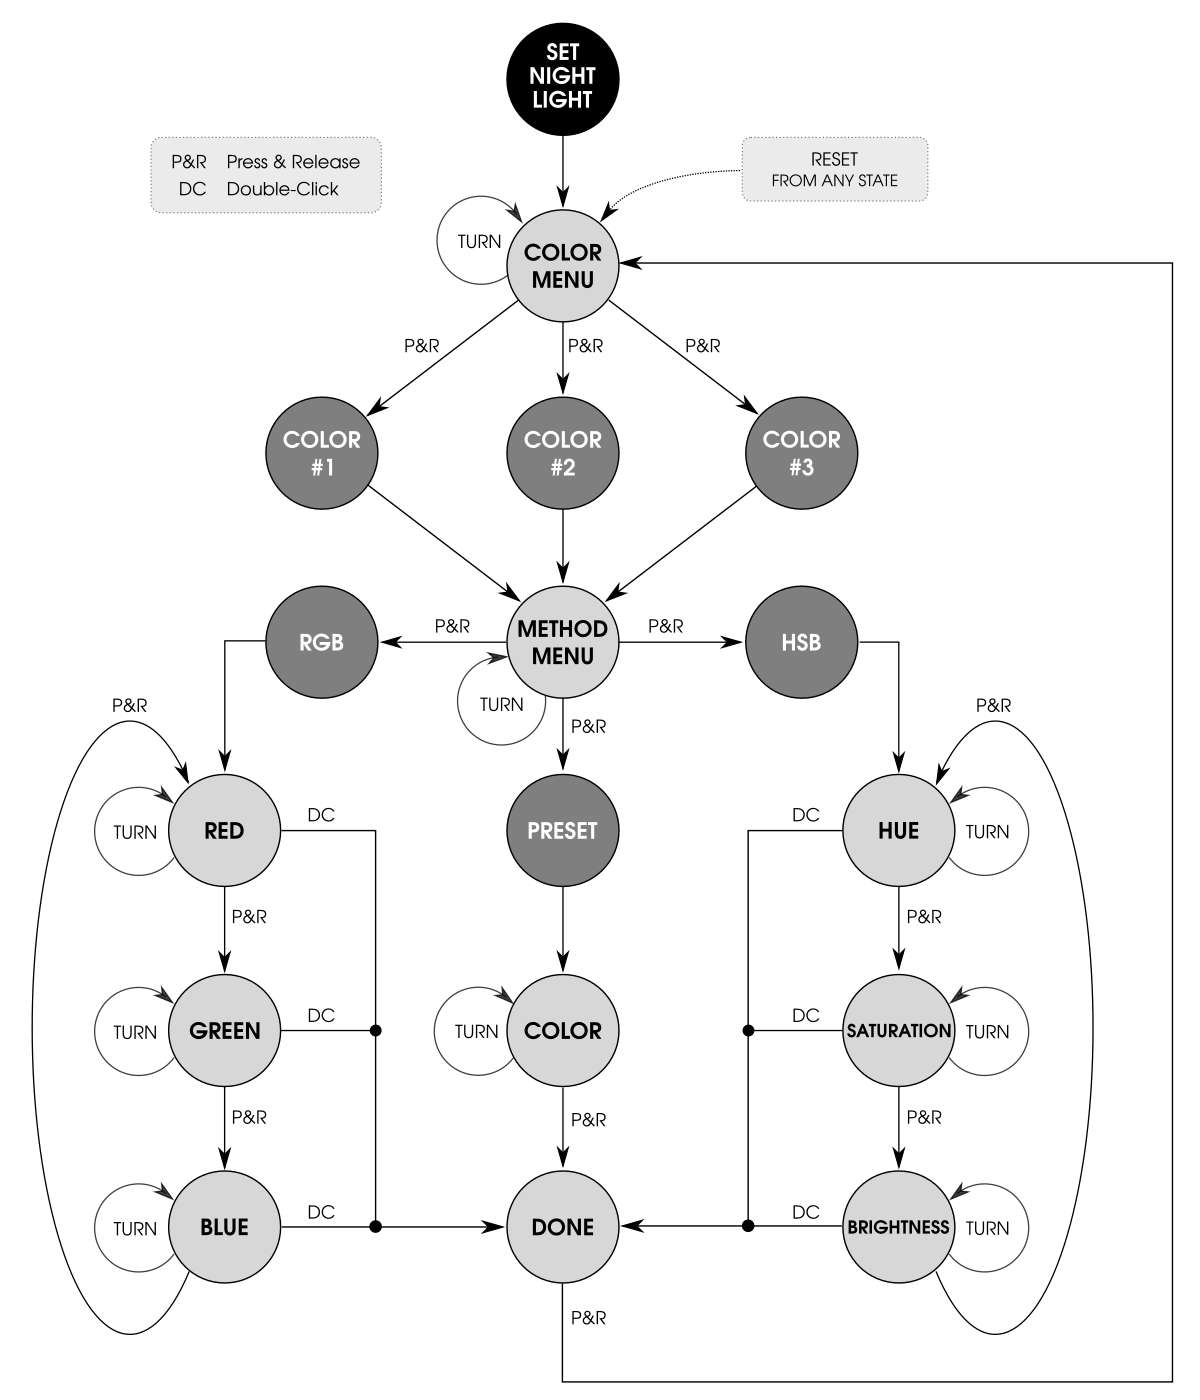
\includegraphics{images/set_night_light_state_diagram.png}
\caption{Set Night Light - State Diagram}
\end{figure}


%%%%%%%%%%%%%%%%%%%%%%%%%%%%%%%%%%%%%%%%%%%%%%%%%%%%%%%%%%%%%%%%%%%%%%%%%%%%%%%%
% Maintenance
%%%%%%%%%%%%%%%%%%%%%%%%%%%%%%%%%%%%%%%%%%%%%%%%%%%%%%%%%%%%%%%%%%%%%%%%%%%%%%%%
%%%%%%%%%%%%%%%%%%%%%%%%%%%%%%%%%%%%%%%%%%%%%%%%%%%%%%%%%%%%%%%%%%%%%%%%%%%%%%%%%
% Maintenance
%%%%%%%%%%%%%%%%%%%%%%%%%%%%%%%%%%%%%%%%%%%%%%%%%%%%%%%%%%%%%%%%%%%%%%%%%%%%%%%%%
\part{Maintenance} \label{Maintenance}

%%%%%%%%%%%%%%%%%%%%%%%%%%%%%%%%%%%%%%%%%%%%%%%%%%%%%%%%%%%%%%%%%%%%%%%%%%%%%%%%
% Cleaning
%%%%%%%%%%%%%%%%%%%%%%%%%%%%%%%%%%%%%%%%%%%%%%%%%%%%%%%%%%%%%%%%%%%%%%%%%%%%%%%%
\chapter{Cleaning} \label{Cleaning}

A dry or slightly damp rag, preferably microfiber, should be sufficient to get
fingerprints, dust and other crud off of the wood finish and \front{} front.

\par\bigskip

\danger{%
\textbf{\fontTGA{l}{ALCOHOL WILL RUIN THE FINISH} \raisebox{-0.5mm}{\huge !}}
\par\medskip
Do \textit{not} use alcohol or any cleaning solution containing alcohol.  It
will dissolve the shellac finish on the wood.  And to be safe, stay away from
chemical cleaning solutions altogether.}

\par\bigskip

Unless you are just giving it a quick, dry wipe-down, before cleaning:
\begin{enumerate}
  \item Switch the device \sOff{f} using the \hyperref[Power Switch]{\cPo{f}}.
  \item Unplug the \hyperref[Power Adapter]{\cPA{f}} from the
    \hyperref[USB Port]{\cPP{f}}.
\end{enumerate}

%%%%%%%%%%%%%%%%%%%%%%%%%%%%%%%%%%%%%%%%%%%%%%%%%%%%%%%%%%%%%%%%%%%%%%%%%%%%%%%%
% Disassembly
%%%%%%%%%%%%%%%%%%%%%%%%%%%%%%%%%%%%%%%%%%%%%%%%%%%%%%%%%%%%%%%%%%%%%%%%%%%%%%%%
\chapter{Disassembly} \label{Disassembly}

Disassembly should only be necessary once every several years to change the
\cCC{f}.  The \cMSD{f} should last for quite a while and should not need
replacement for many years.

%%%%%%%%%%%%%%%%%%%%%%%%%%%%%%%%%%%%%%%%%%%%%%%%%%%%%%%%%%%%%%%%%%%%%%%%%%%%%%%%
% Disassembly - Warnings
%%%%%%%%%%%%%%%%%%%%%%%%%%%%%%%%%%%%%%%%%%%%%%%%%%%%%%%%%%%%%%%%%%%%%%%%%%%%%%%%
\section{Warnings}

Please read and heed these warnings.  The device can be damaged if you do not.

\danger{Be extra careful when removing the screws.  This can't be stressed
enough.  Righty-tighty, lefty-loosey.  If you right-tighty when you should be
lefty-looseying, the screw \textit{\bfseries will strip} the threads in the
wood.}

\warning{When removing the screws take note of which screws came out of which
holes.  When initially tapping the holes, threads may have been stripped in one
or more of the holes requiring a deeper hole and a longer screw.}

\danger{Take care when lifting the \cTo{f} off.  The wires attaching the \cTS{f}
and \cCC{f} to the \cMi{f} are attached from the \cTo{f} to the circuit board on
the \cBa{f}.  The wires are long enough to take it off, turn it over and set it
on top of the open enclosure.  But the fit may be tight and it may not simply
come off, and pulling it off too abruptly may result in an upward force
proportional to the frictional force that was making it difficult to pull off in
the first place resulting in the wires getting torn from their connections.}

\danger{Be extra careful when reassembling.  As soon as you feel \textit{any}
pressure when turning a screw - \textit{\bfseries stop}.  If you continue, the
threads in the wood \textit{\bfseries will be stripped} and the screw will no
longer hold.}

\danger{When reassembling, do \textit{not} rely on the screws pulling the
enclosure together.  Make sure all pieces are tight and flush \textit{before}
tightening the screws.}

\danger{\textbf{\fontTGA{l}{DO NOT USE POWER TOOLS} \raisebox{-0.5mm}{\huge !}}}

%%%%%%%%%%%%%%%%%%%%%%%%%%%%%%%%%%%%%%%%%%%%%%%%%%%%%%%%%%%%%%%%%%%%%%%%%%%%%%%%
% Disassembly - Tools
%%%%%%%%%%%%%%%%%%%%%%%%%%%%%%%%%%%%%%%%%%%%%%%%%%%%%%%%%%%%%%%%%%%%%%%%%%%%%%%%
\section{Tools}

Only one tool is required - a \mono{3/32"} Hex Driver.  However, it is
recommended that you have handy pencil and paper to keep track of which holes
the screws came out of.

\begin{table}[H]
\ers{1}
\centering
\begin{tabu} { X[1,r,m] | X[6,l,m] }
  \thrule
  \thbi{Quantity} & \thbi{Item} \\ \mrule
  1 & \mono{3/32"} Hex Driver, T-handle or Key \\ \drule{2}
  1 & Pen or pencil \\ \drule{2}
  1 & Piece of paper \\
  \bhrule
\end{tabu}
\end{table}

%%%%%%%%%%%%%%%%%%%%%%%%%%%%%%%%%%%%%%%%%%%%%%%%%%%%%%%%%%%%%%%%%%%%%%%%%%%%%%%%
% Disassembly - Top Removal
%%%%%%%%%%%%%%%%%%%%%%%%%%%%%%%%%%%%%%%%%%%%%%%%%%%%%%%%%%%%%%%%%%%%%%%%%%%%%%%%
\section{Top Removal} \label{Top Removal}

To remove the \cTo{f}, you will need to remove the \num{4} screws that attach
the \cSi{f} to the \cTo{f}.  The order of removal is unimportant.  The \cTo{f}
will then be turned, flipped and placed on top of the enclosure.

\warning{Do the following before proceeding:
\begin{enumerate}
  \item Switch the device \sOff{f} using the \hyperref[Power Switch]{\cPo{f}}.
  \item Unplug the \hyperref[Power Adapter]{\cPA{f}} from the
    \hyperref[USB Port]{\cPP{f}}.
\end{enumerate}}

%%%%%%%%%%%%%%%%%%%%%%%%%%%%%%%%%%%%%%%%%%%%%%%%%%%%%%%%%%%%%%%%%%%%%%%%%%%%%%%%
% Disassembly - Top Removal - Removing the Screws
%%%%%%%%%%%%%%%%%%%%%%%%%%%%%%%%%%%%%%%%%%%%%%%%%%%%%%%%%%%%%%%%%%%%%%%%%%%%%%%%
\subsection{Removing the Screws} \label{Removing the Screws}

The screws used are technically machine screws which are generally used with
metals, however the wood used for the enclosure is sufficiently dense. Machine
screws are used so that the device can be easily taken apart and put back
together - though care must be taken when doing so.

\par\medskip

Utilizing machine screws as opposed to self-tapping wood screws involves a
different process.  First a hole is drilled, much like a pilot hole for a
self-tapping wood screw, but instead of using a screw driver to drive the screw
in, a tap and tap driver is used to create the threads in the hole.

\par\medskip

Despite the wood being very dense, it is very easy to strip the threads if
overtightned - either when loosening and turning the wrong way or when
tightening.  So go slow, very slow, and as soon as you feel
\textit{\bfseries any resistance, stop turning}.

\steps{Removing Screws}{%
\begin{enumerate}
  \item Orient the enclosure so that you are \textit{facing} the screw you
    will be loosening.
  \item Insert the \mono{3/32"} Hex Driver into the head of the screw.
  \item \textit{Slowly} turn \textit{counter-clockwise} until the screw is
    \textit{completely} loosened and pull it out.

  \begin{figure}[H]
  \centering
    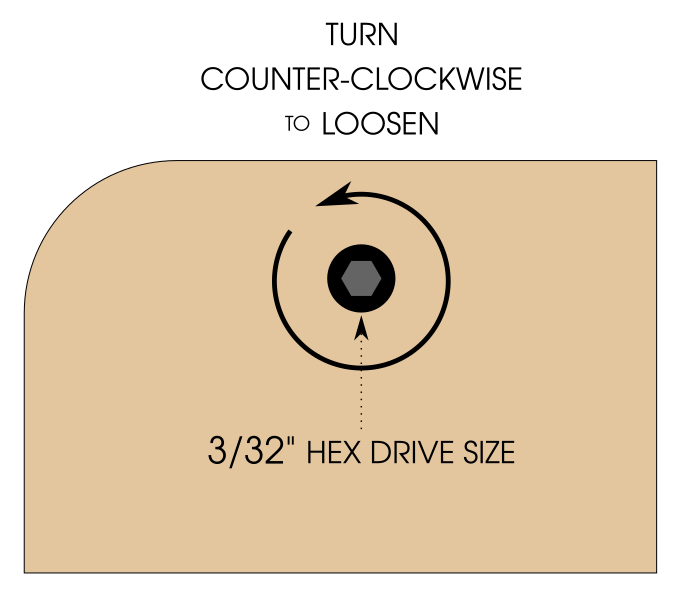
\includegraphics{images/disassembly_loosen.png}
  %\caption{Disassembly - Loosen Screws}
  \end{figure}

  \item Make a note with pencil and paper of the hole the screw came out of and
    place the screw next to or on top of it.
  \item Repeat the above steps for all screws to be removed.
\end{enumerate}}

\info{If removing the \cMSD{f}, in addition to removing the \num{4} screws
attaching the \cSi{f} to the \cTo{f}, you may need to remove the \num{2} screws
attaching the \cLS{f} to the \cBo{f}.}

%%%%%%%%%%%%%%%%%%%%%%%%%%%%%%%%%%%%%%%%%%%%%%%%%%%%%%%%%%%%%%%%%%%%%%%%%%%%%%%%
% Disassembly - Top Removal - Top Placement
%%%%%%%%%%%%%%%%%%%%%%%%%%%%%%%%%%%%%%%%%%%%%%%%%%%%%%%%%%%%%%%%%%%%%%%%%%%%%%%%
\subsection{Top Placement}

After removing the screws, you will lift the \cTo{f}, turn it over and place
it on top of the enclosure, sitting perpendicular to its attached orientation.

\steps{Top Placement}{%
\begin{enumerate}
  \item \textit{Slowly} pull the \cTo{f} up.  If there is resistance,
    \textit{gently} rock the \cTo{f} from side to side to loosen it until it
    easily detaches.
  \item Lift it \textit{no more} than about \mono{1"} above the enclosure - just
    high enough to be able to turn it perpendicular to the way it is oriented.

  \begin{figure}[H]
  \centering
    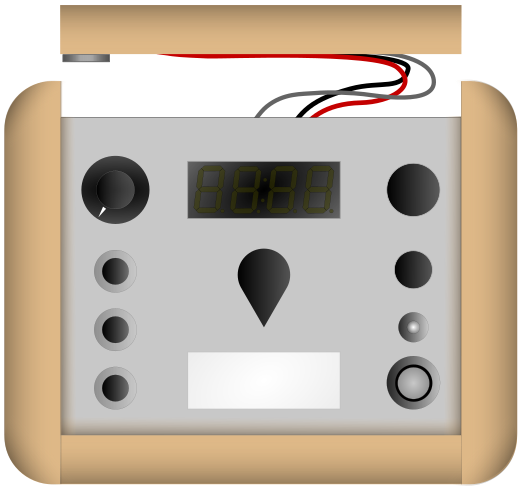
\includegraphics{images/disassembly_01.png}
  \end{figure}

  \item Facing front and looking down, turn the \cTo{f}
    \textit{counter-clockwise} until it is perpendicular to its attached
    orientation.

  \begin{figure}[H]
  \centering
    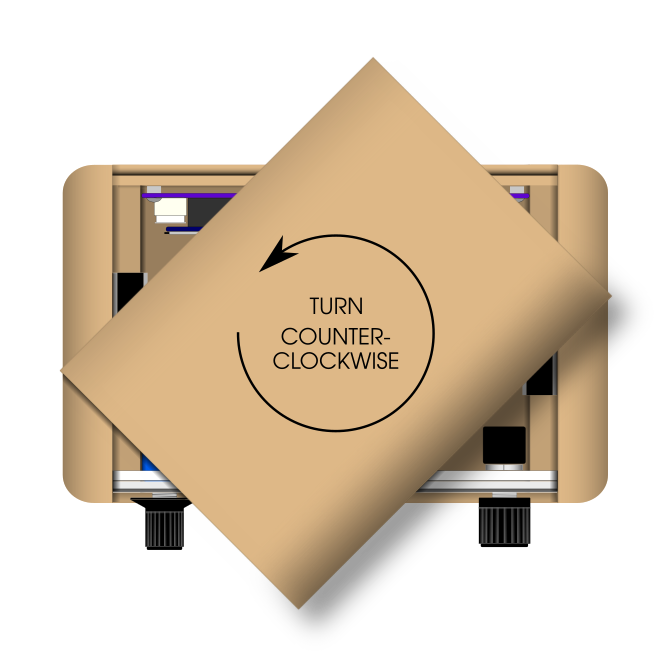
\includegraphics{images/disassembly_02.png}
  \end{figure}

  \item Facing front, flip the \cTo{f} \textit{clockwise}.

  \begin{figure}[H]
  \centering
    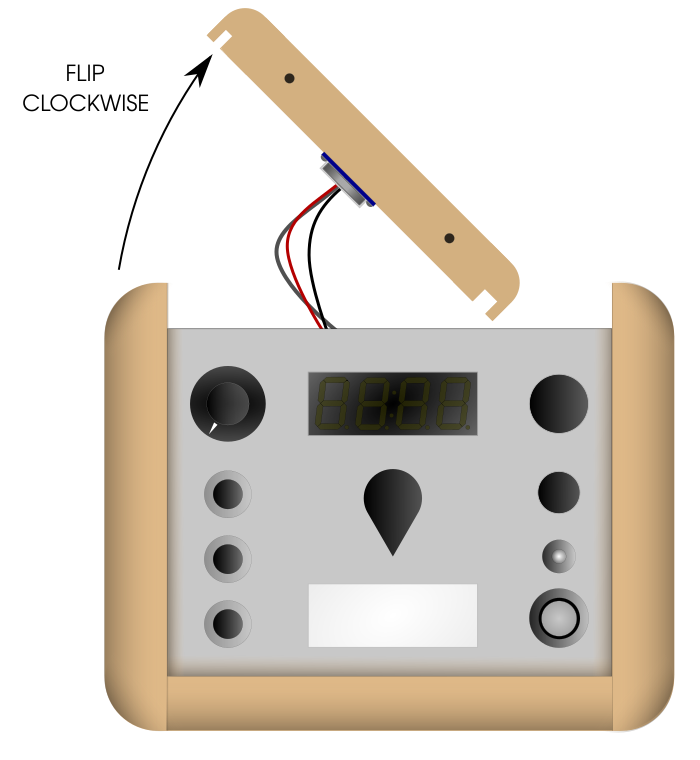
\includegraphics{images/disassembly_03.png}
  \end{figure}

  \item \textit{Gently} place it on top of the enclosure.

  \begin{figure}[H]
  \centering
    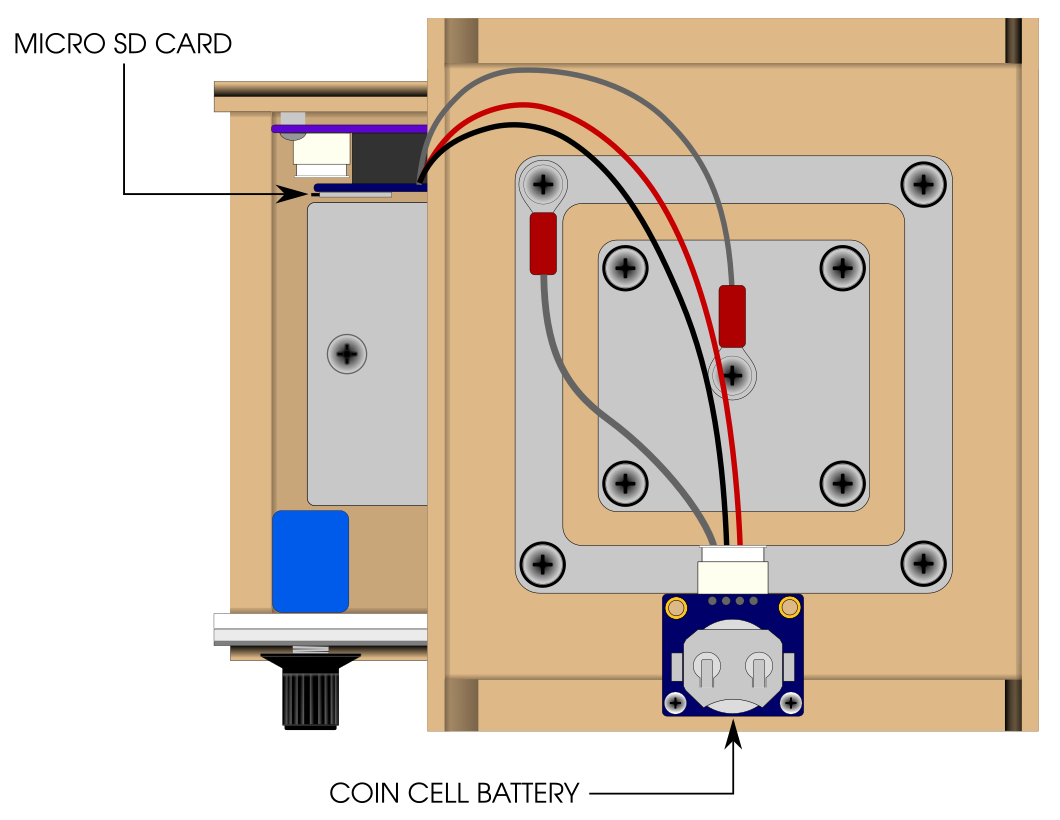
\includegraphics{images/disassembly_04.png}
  \end{figure}

\end{enumerate}}

%%%%%%%%%%%%%%%%%%%%%%%%%%%%%%%%%%%%%%%%%%%%%%%%%%%%%%%%%%%%%%%%%%%%%%%%%%%%%%%%
% Disassembly - Reassembly
%%%%%%%%%%%%%%%%%%%%%%%%%%%%%%%%%%%%%%%%%%%%%%%%%%%%%%%%%%%%%%%%%%%%%%%%%%%%%%%%
\section{Reassembly} \label{Reassembly}

Place the \cTo{f} and possibly the \cLS{f}, if it was necessary to remove to
get to the \cMSD{f}, back in place.  Make sure all wires are \textit{within} the
enclosure so that they are not crimped when placing the pieces back together and
that all pieces are tight and flush before putting the screws back in and
tightening.

\par\medskip

Again, go slow, very slow, when tightening the screws and as soon as you feel
\textit{\bfseries any resistance, stop turning}.

\steps{Tightening Screws}{%
\begin{enumerate}
  \item Make sure the \cTo{f} and \cSi{f} are tight and flush.
  \item Orient the enclosure so that you are \textit{facing} the screw you
    will be tightening.
  \item Insert the screw into the hole - make sure it is the same screw that
    came out of the hole.
  \item Insert the \mono{3/32"} Hex Driver into the head of the screw.
  \item \textit{Slowly} turn \textit{clockwise}.  As soon as you feel
    \textit{any resistance}, \textit{\bfseries stop} turning.

  \begin{figure}[H]
  \centering
    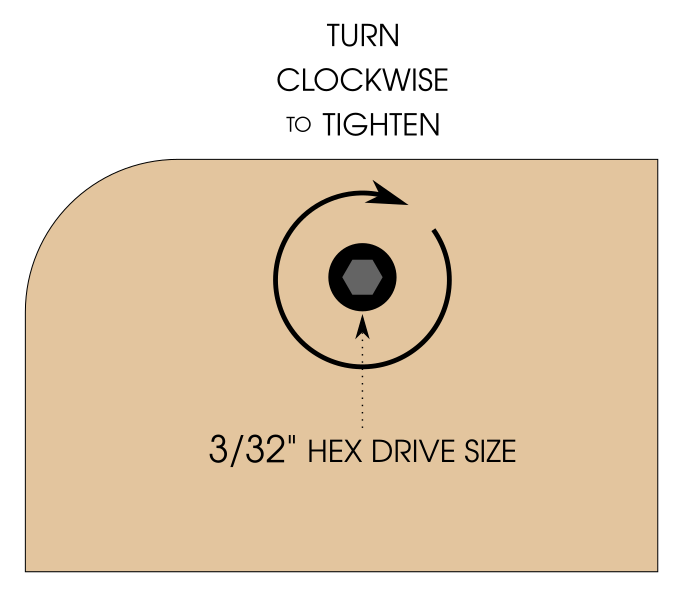
\includegraphics{images/disassembly_tighten.png}
  %\caption{Reassembly - Tighten Screws}
  \end{figure}

  \item Repeat the above steps for all removed screws.
\end{enumerate}}

%%%%%%%%%%%%%%%%%%%%%%%%%%%%%%%%%%%%%%%%%%%%%%%%%%%%%%%%%%%%%%%%%%%%%%%%%%%%%%%%
% Replacing the Coin Cell Battery
%%%%%%%%%%%%%%%%%%%%%%%%%%%%%%%%%%%%%%%%%%%%%%%%%%%%%%%%%%%%%%%%%%%%%%%%%%%%%%%%
\chapter{Replacing the Coin Cell Battery} \label{Replacing Battery}

Replacing the \hyperref[Coin Cell Battery]{\cCC{f}} shouldn't be necessary for
several years.  It is a \num{CR2032} and is located just underneath the \cTo{f}
on the \textit{left} side.  To access the battery, the \cTo{f} needs to be
removed - refer to the \hyperref[Disassembly]{Disassembly} section for
instructions.

%%%%%%%%%%%%%%%%%%%%%%%%%%%%%%%%%%%%%%%%%%%%%%%%%%%%%%%%%%%%%%%%%%%%%%%%%%%%%%%%
% Replacing the Coin Cell Battery - Parts
%%%%%%%%%%%%%%%%%%%%%%%%%%%%%%%%%%%%%%%%%%%%%%%%%%%%%%%%%%%%%%%%%%%%%%%%%%%%%%%%
\section{Parts}

One \mono{CR2032} coin cell battery is necessary.

\begin{table}[H]
\ers{1}
\centering
\begin{tabu} { X[1,r,m] | X[6,l,m] }
  \thrule
  \thbi{Quantity} & \thbi{Part} \\ \mrule
  1 & \mono{CR2032} (\mono{3\thinspace V}) Coin Cell Battery \\
  \bhrule
\end{tabu}
\end{table}

%%%%%%%%%%%%%%%%%%%%%%%%%%%%%%%%%%%%%%%%%%%%%%%%%%%%%%%%%%%%%%%%%%%%%%%%%%%%%%%%
% Replacing the Coin Cell Battery - Removal
%%%%%%%%%%%%%%%%%%%%%%%%%%%%%%%%%%%%%%%%%%%%%%%%%%%%%%%%%%%%%%%%%%%%%%%%%%%%%%%%
\section{Removal}

To remove the \cCC{f}, simply push it from within the bounds of the \cTo{f}
towards the outside.

\begin{figure}[H]
\centering
  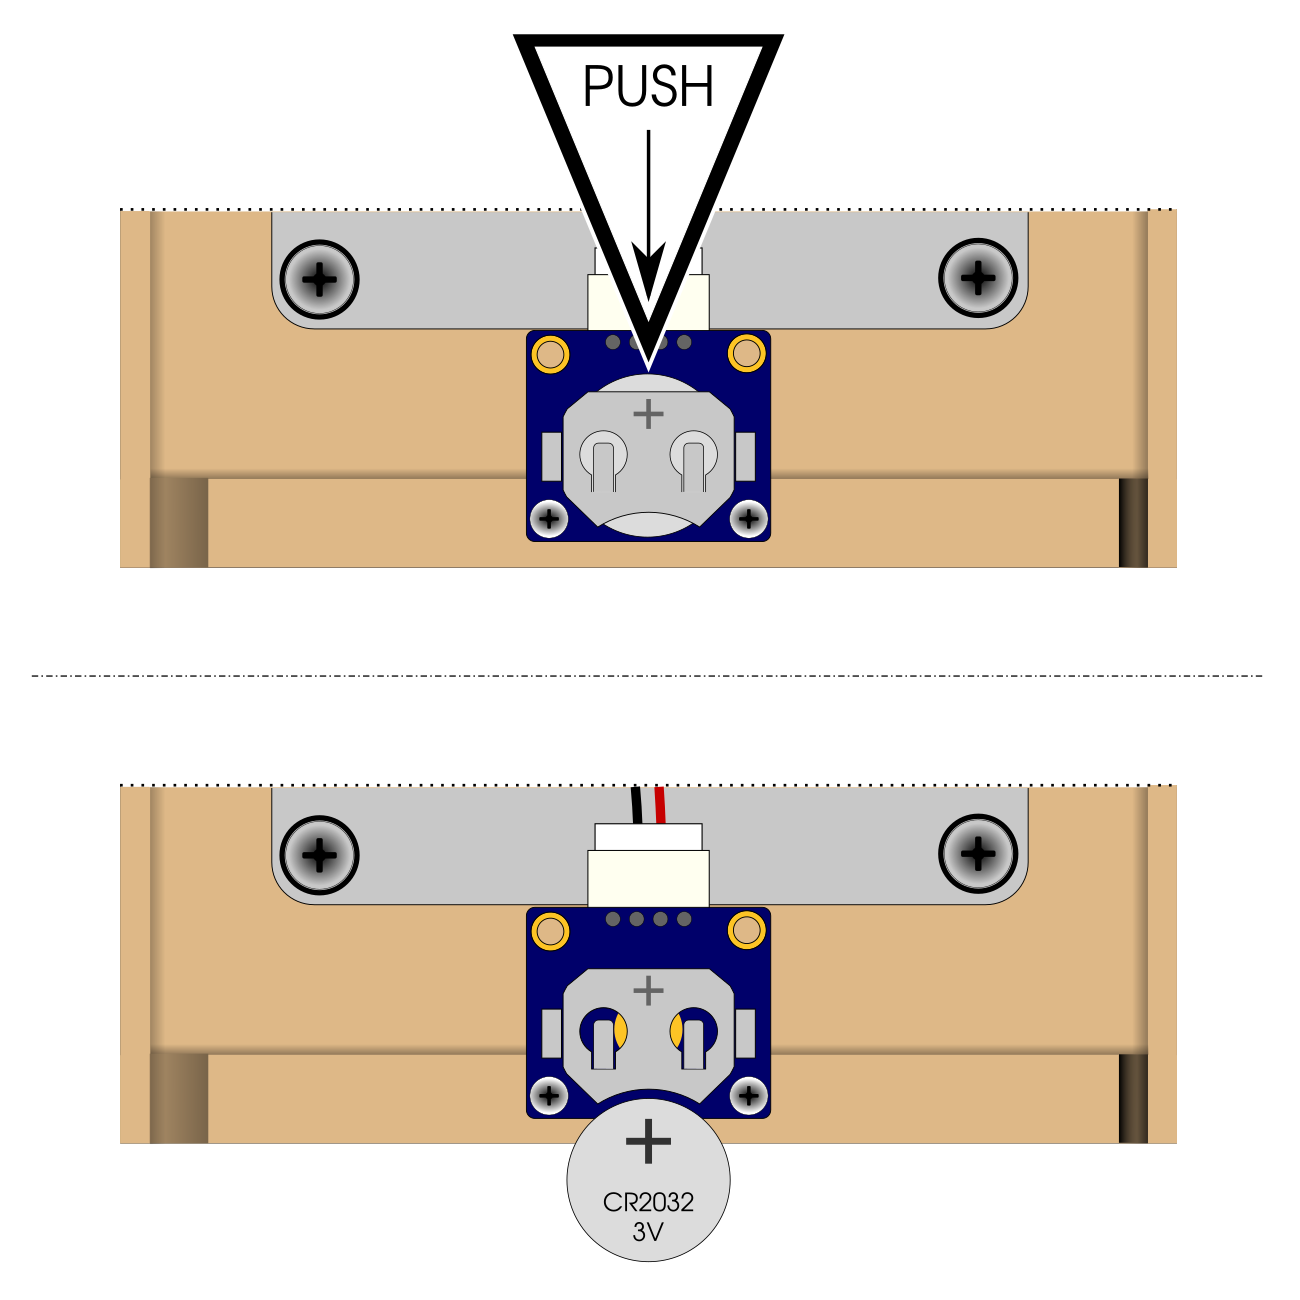
\includegraphics{images/coin_cell_battery.png}
\caption{Removing the Coin Cell Battery}
\end{figure}

%%%%%%%%%%%%%%%%%%%%%%%%%%%%%%%%%%%%%%%%%%%%%%%%%%%%%%%%%%%%%%%%%%%%%%%%%%%%%%%%
% Replacing the Coin Cell Battery - Insertion
%%%%%%%%%%%%%%%%%%%%%%%%%%%%%%%%%%%%%%%%%%%%%%%%%%%%%%%%%%%%%%%%%%%%%%%%%%%%%%%%
\section{Insertion} \label{SD Insertion}

\danger{When inserting the new battery, orientation is critical.  If the
polarity is reversed, damage may occur.}

Before inserting the new battery, make sure the
\begin{tikzpicture}[baseline=-4]
  \draw[fill=black!20] (0,0) circle [radius=0.4] node[anchor=center] {\textbf{\Large{$+$}}};
\end{tikzpicture}
or positive side of the battery is \textit{facing up}.  After verifying this,
simply push it in the way it came out.

%%%%%%%%%%%%%%%%%%%%%%%%%%%%%%%%%%%%%%%%%%%%%%%%%%%%%%%%%%%%%%%%%%%%%%%%%%%%%%%%
% Removing the Micro SD Card
%%%%%%%%%%%%%%%%%%%%%%%%%%%%%%%%%%%%%%%%%%%%%%%%%%%%%%%%%%%%%%%%%%%%%%%%%%%%%%%%
\chapter{Removing the Micro SD Card} \label{Removing SD Card}

%Though it's possible and relatively easy to do, the device was not conceived
%to add and remove songs from the \cMSD{f}.

The \cMSD{f} is held in place by a spring clip attached to a part on the circuit
board.  Removal involves pushing the card inward until you hear a
\textit{click}, then releasing.  The card will be partially pushed out by the
spring clip.  You can then pull the card out the rest of the way.  To put the
card back in, push until you hear a \textit{click} and it will catch into place.
Verify that it is in place by gently pulling on it - it should \textit{not} pull
out.

\par\medskip

Before the \cMSD{f} can be removed, the enclosure needs to be partially
disassembled - refer to \hyperref[Disassembly]{Disassembly} for instructions.

\info{You may need to detach the \cLS{f} to get to the card.  If so remove the
\num{2} screws that attach the \cLS{f} to the \cBo{f} in addition to the \num{4}
that attach the \cSi{f} to the \cTo{f} -
see \hyperref[Removing the Screws]{Removing the screws} in the
\hyperref[Top Removal]{Top Removal} section.}

\begin{figure}[H]
\centering
  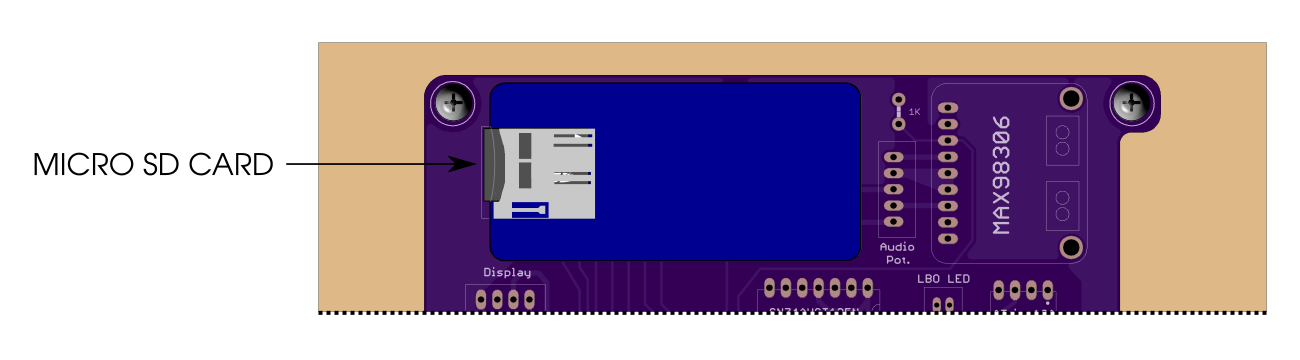
\includegraphics{images/micro_sd_card.png}
\caption{Micro SD Card - Location}
\end{figure}

%%%%%%%%%%%%%%%%%%%%%%%%%%%%%%%%%%%%%%%%%%%%%%%%%%%%%%%%%%%%%%%%%%%%%%%%%%%%%%%%
% Removing the Micro SD Card - Removal
%%%%%%%%%%%%%%%%%%%%%%%%%%%%%%%%%%%%%%%%%%%%%%%%%%%%%%%%%%%%%%%%%%%%%%%%%%%%%%%%
\pagebreak
\section{Removal} \label{SD Removal}

\steps{Micro SD Card Removal}{%
\begin{enumerate}
  \item Push the \cMSD{f} inward until you hear a \textit{click}.
    \begin{figure}[H]
    \centering
      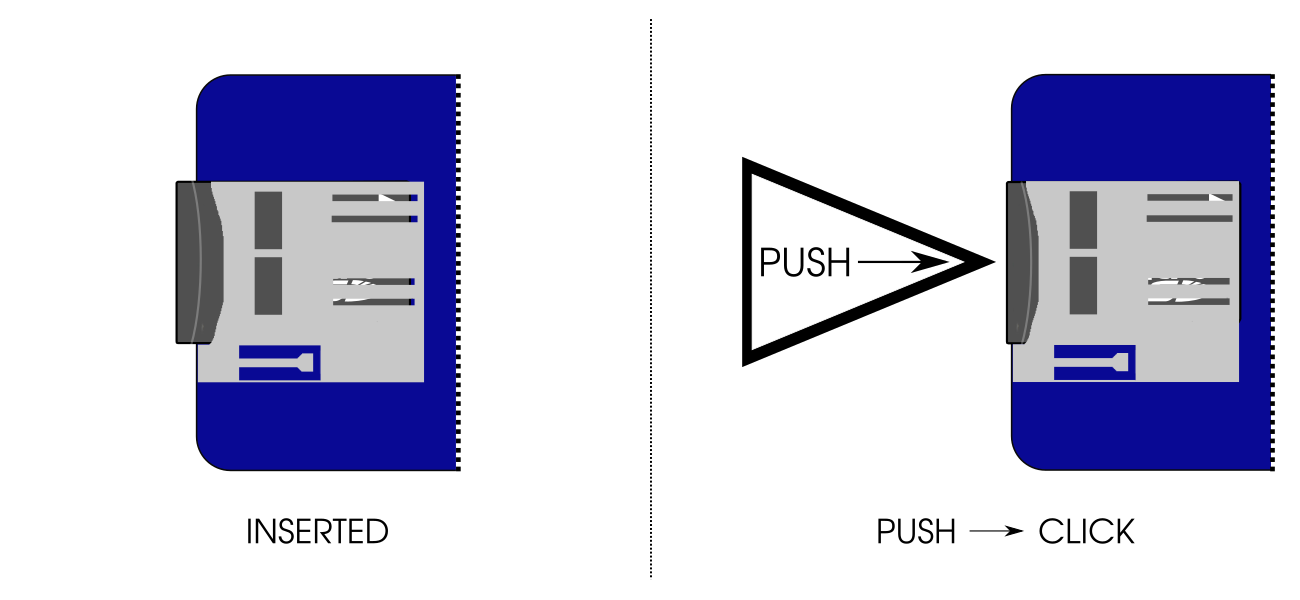
\includegraphics{images/micro_sd_card_removal_01.png}
    \end{figure}
    \par\bigskip
  \item Release and the card will be partially pushed out.
    \begin{figure}[H]
    \centering
      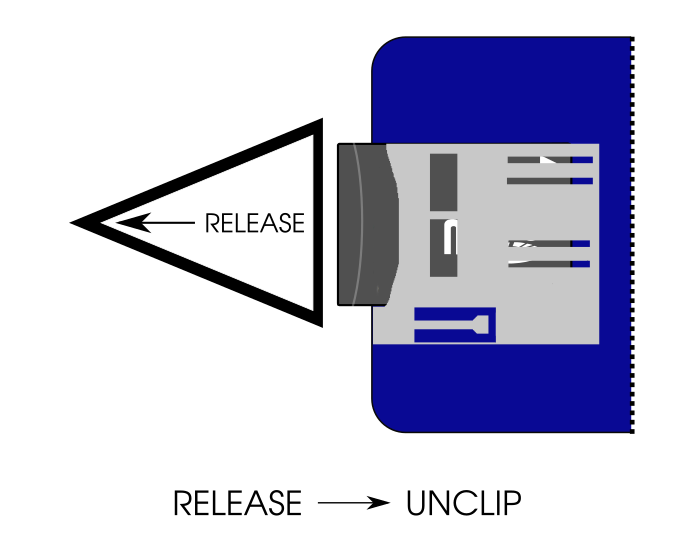
\includegraphics{images/micro_sd_card_removal_02.png}
    \end{figure}
    \par\bigskip
  \pagebreak
  \item Pull the card out the rest of the way.
    \begin{figure}[H]
    \centering
      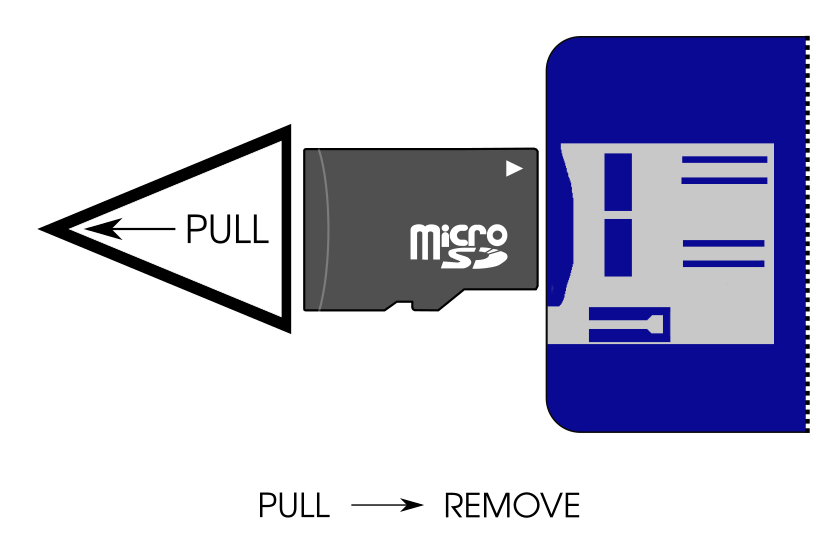
\includegraphics{images/micro_sd_card_removal_03.png}
    \end{figure}
\end{enumerate}}

%%%%%%%%%%%%%%%%%%%%%%%%%%%%%%%%%%%%%%%%%%%%%%%%%%%%%%%%%%%%%%%%%%%%%%%%%%%%%%%%
% Removing the Micro SD Card - Insertion
%%%%%%%%%%%%%%%%%%%%%%%%%%%%%%%%%%%%%%%%%%%%%%%%%%%%%%%%%%%%%%%%%%%%%%%%%%%%%%%%
\section{Insertion}

\steps{Micro SD Card Insertion}{%
\begin{enumerate}
  \item Push the \cMSD{f} inward until you hear a \textit{click}.
    \begin{figure}[H]
    \centering
      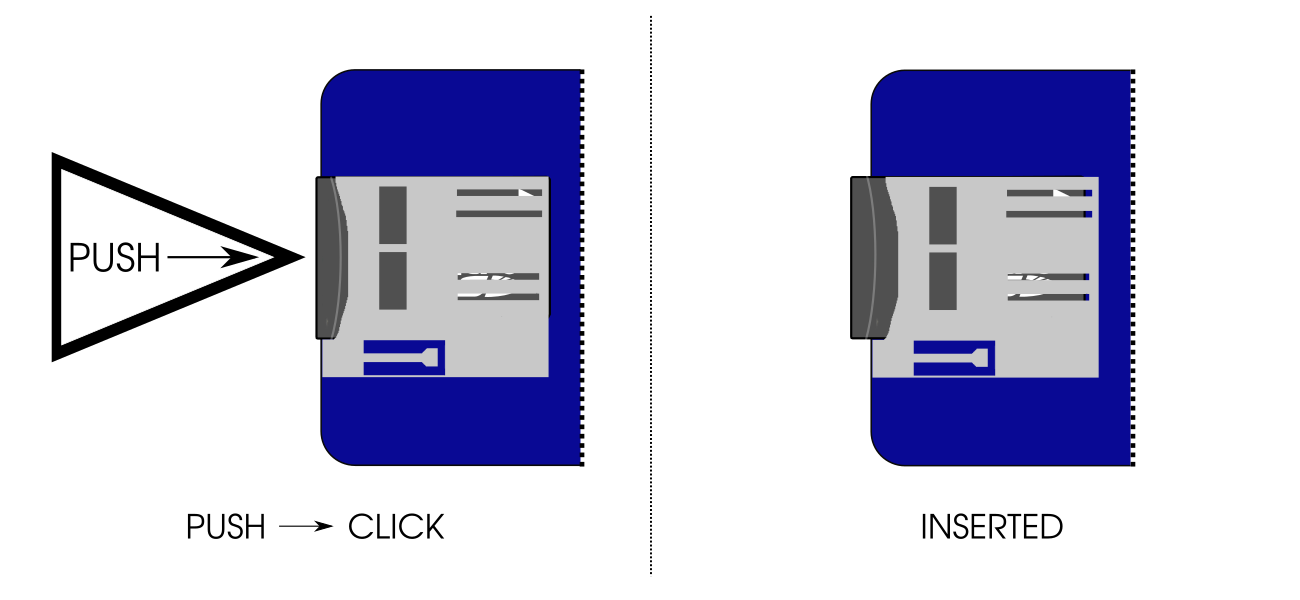
\includegraphics{images/micro_sd_card_insertion.png}
    \end{figure}
\end{enumerate}}

\iffalse
% Adding USB capability deprecates the following section which requires
% removing the microSD card in order to add and remove songs.  However,
% do not remove it in case USB capability is not compiled in.
 
%%%%%%%%%%%%%%%%%%%%%%%%%%%%%%%%%%%%%%%%%%%%%%%%%%%%%%%%%%%%%%%%%%%%%%%%%%%%%%%%
% Removing the Micro SD Card - Adding / Removing Songs
%%%%%%%%%%%%%%%%%%%%%%%%%%%%%%%%%%%%%%%%%%%%%%%%%%%%%%%%%%%%%%%%%%%%%%%%%%%%%%%%
\pagebreak
\section{Adding / Removing Songs} \label{Add Songs}

Disassembly is primarily meant for maintenance and changing the \cCC{f}
and should \textit{not} be done often.  Unfortunately the only way to
add / remove songs from the \cMSD{f} is to partially disassemble the enclosure
- see \hyperref[Disassembly]{Disassembly} for instructions.

\par\medskip

There are a number of ways to add files to the \cMSD{f}.  It will be assumed
that a desktop or laptop computer with a windowed environment is being used
such as a Mac or Windows.

%%%%%%%%%%%%%%%%%%%%%%%%%%%%%%%%%%%%%%%%%%%%%%%%%%%%%%%%%%%%%%%%%%%%%%%%%%%%%%%%
% Removing the Micro SD Card - Adding / Removing Songs - Preparation
%%%%%%%%%%%%%%%%%%%%%%%%%%%%%%%%%%%%%%%%%%%%%%%%%%%%%%%%%%%%%%%%%%%%%%%%%%%%%%%%
\subsection{Preparation}

Preparation involves partially disassembling the enclosure, removing the
\cMSD{f} from the holder on the circuit board and attaching the card to a
computer.

\steps{Preparation}{%
\begin{enumerate}
  \item Partially disassemble the enclosure - refer to
    \hyperref[Disassembly]{Disassembly} for instructions.
  \item Remove the \cMSD{f} - refer to \hyperref[SD Removal]{Removal} for
    instructions.
  \item Insert the card into the computer.  There are a couple of ways this
    may be accomplished.
    \begin{itemize}
      \item If your computer has a built-in \cMSD{f} reader, you should be
        able to use that.
      \item Use a USB card reader.\footnote{ One that I have used without issue
        is \mono{Transcend RDF5}.}  After inserting the card into the reader,
        insert the reader into a USB port on the computer.
    \end{itemize}
  \item The card should be recognized as a disk volume on the computer.  The
    card that comes pre-installed is named \mono{MUSIC}.  Open a window that
    shows the contents of the disk.
\end{enumerate}}

%%%%%%%%%%%%%%%%%%%%%%%%%%%%%%%%%%%%%%%%%%%%%%%%%%%%%%%%%%%%%%%%%%%%%%%%%%%%%%%%
% Removing the Micro SD Card - Adding / Removing Songs - Adding Files
%%%%%%%%%%%%%%%%%%%%%%%%%%%%%%%%%%%%%%%%%%%%%%%%%%%%%%%%%%%%%%%%%%%%%%%%%%%%%%%%
\subsection{Adding Songs} \label{Adding Songs}

Adding songs involves copying \mono{MP3} or \mono{M4A} music files that are on
a computer to the \cMSD{f}.

\warning{The files \textit{must} be \mono{MPEG-2 Audio Layer III} (\mono{MP3})
or \mono{MPEG-4 Audio}\footnote{ Used primarily by iTunes.} (\mono{M4A}) files
and they \textit{must} have an \mono{.mp3} or \mono{.m4a} file extension.
Files that are \textit{not} \mono{MP3} or \mono{M4A} and that do \textit{not}
have either of the two file extensions in the file name will \textit{not} work.}

\steps{Adding Songs}{%
\begin{enumerate}
  \item Open another window that has the songs you want to add.
  \item Drag and drop the \mono{MP3} and/or \mono{M4A} files you want to add
    onto the \cMSD{f} volume.
    \par\medskip
    Note that the disk has no concept of sorting and the order in which the
    songs are ``sorted'' on the disk is the order in which they are added to
    the disk.  If you want the songs to be played in a specific order,
    add them \textit{one at a time} to the \cMSD{f}.
\end{enumerate}}

%%%%%%%%%%%%%%%%%%%%%%%%%%%%%%%%%%%%%%%%%%%%%%%%%%%%%%%%%%%%%%%%%%%%%%%%%%%%%%%%
% Removing the Micro SD Card - Adding / Removing Songs - Removing Files
%%%%%%%%%%%%%%%%%%%%%%%%%%%%%%%%%%%%%%%%%%%%%%%%%%%%%%%%%%%%%%%%%%%%%%%%%%%%%%%%
\subsection{Removing Songs}

Removing songs simply involves deleting the files from the \cMSD{f}.

\steps{Removing Songs}{%
\begin{enumerate}
  \item Delete or ``Move to Trash'' the files you want removed from the
    \cMSD{f} volume.
\end{enumerate}}

%%%%%%%%%%%%%%%%%%%%%%%%%%%%%%%%%%%%%%%%%%%%%%%%%%%%%%%%%%%%%%%%%%%%%%%%%%%%%%%%
% Removing the Micro SD Card - Adding / Removing Songs - Finishing
%%%%%%%%%%%%%%%%%%%%%%%%%%%%%%%%%%%%%%%%%%%%%%%%%%%%%%%%%%%%%%%%%%%%%%%%%%%%%%%%
\subsection{Finishing}

Finishing involves ejecting then physically removing the \cMSD{f} from the
computer, putting it back in the holder on the circuit board and closing up the
enclosure.

\steps{Finishing}{%
\begin{enumerate}
  \item Safely remove or eject the \cMSD{f}. This is \textit{not} physical
    removal but tells the computer to finish any possible pending
    operations, such as writes to the disk, \textit{before} physical removal.
  \item Physically remove the \cMSD{f} from the computer.
  \item Reinsert the \cMSD{f} back into the holder on the circuit board -
    refer to \hyperref[SD Insertion]{Insertion} for instructions.
  \item Reassemble the enclosure - refer to \hyperref[Reassembly]{Reassembly}
    for instructions.
\end{enumerate}}
% Adding USB capability deprecates the above section which requires
% removing the microSD card in order to add and remove songs.  However,
% do not remove it in case USB capability is not compiled in.
\fi

%%%%%%%%%%%%%%%%%%%%%%%%%%%%%%%%%%%%%%%%%%%%%%%%%%%%%%%%%%%%%%%%%%%%%%%%%%%%%%%%
% Removing the Micro SD Card - Replace SD Card
%%%%%%%%%%%%%%%%%%%%%%%%%%%%%%%%%%%%%%%%%%%%%%%%%%%%%%%%%%%%%%%%%%%%%%%%%%%%%%%%
\pagebreak
\section{Replacement} \label{Replace SD Card}

The \cMSD{f} may eventually fail and need to be replaced.  This section will
only focus on formatting the new card.  See the
\hyperref[Disassembly]{Disassembly} section and the preceding sections for
removing the card from the enclosure.

\par\medskip

The new card must meet these requirements.

\begin{itemize}
  \item The card \textit{must} have at least a \num{90} \mono{MB/sec} read
    speed, \textit{and}
  \item The card \textit{must} be formatted with the \mono{FAT32} filesystem
    using \num{512} bytes per sector.
\end{itemize}

\warning{If the read speed of the card is less than \num{90} \mono{MB/sec}, the
audio may stutter and not play correctly.}

\danger{If the card is not formatted with the \mono{FAT32} filesystem using
\num{512} bytes per sector, the device will \textit{not} be able to read the
card.}

%%%%%%%%%%%%%%%%%%%%%%%%%%%%%%%%%%%%%%%%%%%%%%%%%%%%%%%%%%%%%%%%%%%%%%%%%%%%%%%%
% Removing the Micro SD Card - Replace SD Card - Parts
%%%%%%%%%%%%%%%%%%%%%%%%%%%%%%%%%%%%%%%%%%%%%%%%%%%%%%%%%%%%%%%%%%%%%%%%%%%%%%%%
\subsection{Parts}

One Micro SD Card with at least a \num{90} \mono{MB/sec} read speed specification
is needed.

\begin{table}[H]
\ers{1}
\centering
\begin{tabu} { X[1,r,m] | X[6,l,m] }
  \thrule
  \thbi{Quantity} & \thbi{Part} \\ \mrule
  1 & Micro SD Card w/ \num{90} \mono{MB/sec} or more Read Speed \\
  \bhrule
\end{tabu}
\end{table}

A Micro SD Card is distinguished from a normal SD card and the Mini SD Card in
that it is the smallest of the three.

\begin{figure}[H]
\centering
  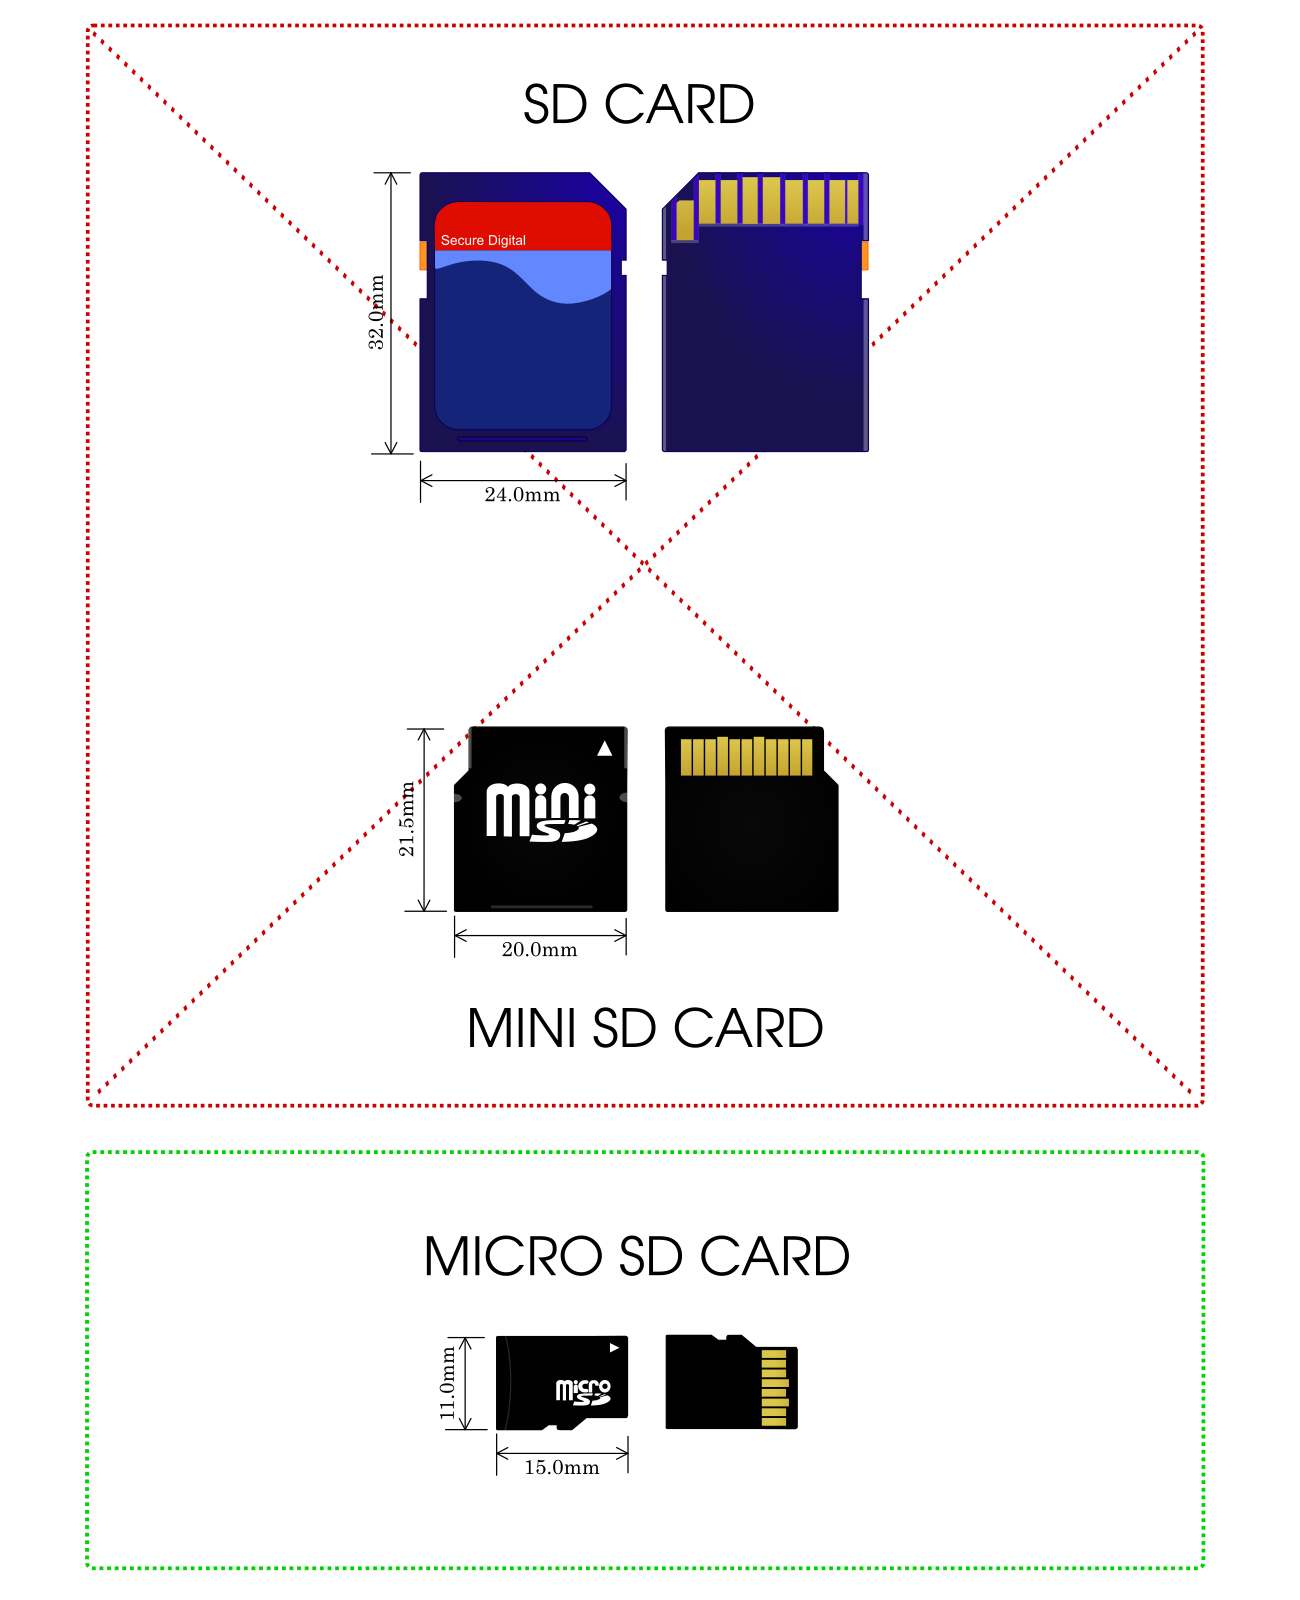
\includegraphics{images/sd_cards.png}
\caption{SD Cards}
\end{figure}

%%%%%%%%%%%%%%%%%%%%%%%%%%%%%%%%%%%%%%%%%%%%%%%%%%%%%%%%%%%%%%%%%%%%%%%%%%%%%%%%
% Removing the Micro SD Card - Replace SD Card - Formatting
%%%%%%%%%%%%%%%%%%%%%%%%%%%%%%%%%%%%%%%%%%%%%%%%%%%%%%%%%%%%%%%%%%%%%%%%%%%%%%%%
\subsection{Formatting}

It is recommended that the
\href{https://www.sdcard.org/downloads/formatter\_4/}{SD Memory Card Formatter}
application be used to format the card.  It is provided for free by the
\href{https://www.sdcard.org/index.html}{SD Association}.  The following will
assume use of this application.

\steps{Download \& Open}{%
\begin{enumerate}
  \item Download the \textit{SD Memory Card Formatter} application from
    \url{https://www.sdcard.org/downloads/formatter\_4/}.  It is available
    for both Windows and Mac so make sure you choose the appropriate download
    for your operating system.
  \item Insert the new \cMSD{f} into the computer.
  \item Open the \textit{SD Memory Card Formatter} application.
\end{enumerate}}

\begin{figure}[H]
\centering
  \includegraphics{images/sd_formatter.png}
\caption{Micro SD Card - SD Memory Card Formatter}
\end{figure}

The window is partitioned into \num{4} sections which will correspond to the
next steps.  Make sure when selecting the card in the first step, that you
select the card you just inserted.  If you select a different card, all of
its contents will be erased.

\danger{Selecting the wrong card will result in erasing the contents
of that card.}

\begin{figure}[H]
\centering
  \includegraphics{images/sd_formatter_steps.png}
\caption{Micro SD Card - Formatting}
\end{figure}

\steps{Format}{%
\begin{enumerate}
  \item \textbf{Select Card} \newline
    Select the card you just inserted from the drop-down menu at the top.  If
    there is more than one choice, make sure you choose the correct card.
  \item \textbf{Select Format Option} \newline
    Leave this alone.
  \item \textbf{Specify Name of Card} \newline
    You can name this anything you like.
  \item \textbf{Click Format button} \newline
    Click on the \cCol{white}{black}{Format}\thinspace button in the lower right.
    Formatting should not take long and when it's finished you should see some
    \textit{blue} text underneath the option indicating success.
\end{enumerate}}

\begin{figure}[H]
\centering
  \includegraphics{images/sd_formatter_success.png}
\caption{Micro SD Card - Formatting Success}
\end{figure}

You can either install the card back in the device or add music directly to the
card while it is out of the device.  Adding songs now will likely be
significantly faster than adding them when the card is in the device, so if
there is a sizeable amount of songs you want to add, it is advisable to add them
now.  See \hyperref[Adding Songs]{Adding Songs} in the \hyperref[USB]{\mUsb{f}}
section.


%%%%%%%%%%%%%%%%%%%%%%%%%%%%%%%%%%%%%%%%%%%%%%%%%%%%%%%%%%%%%%%%%%%%%%%%%%%%%%%%
% Troubleshooting
%%%%%%%%%%%%%%%%%%%%%%%%%%%%%%%%%%%%%%%%%%%%%%%%%%%%%%%%%%%%%%%%%%%%%%%%%%%%%%%%
%%%%%%%%%%%%%%%%%%%%%%%%%%%%%%%%%%%%%%%%%%%%%%%%%%%%%%%%%%%%%%%%%%%%%%%%%%%%%%%%
% Troubleshooting
%%%%%%%%%%%%%%%%%%%%%%%%%%%%%%%%%%%%%%%%%%%%%%%%%%%%%%%%%%%%%%%%%%%%%%%%%%%%%%%%
\part{Troubleshooting} \label{Troubleshooting}

%%%%%%%%%%%%%%%%%%%%%%%%%%%%%%%%%%%%%%%%%%%%%%%%%%%%%%%%%%%%%%%%%%%%%%%%%%%%%%%%
% Common Issues
%%%%%%%%%%%%%%%%%%%%%%%%%%%%%%%%%%%%%%%%%%%%%%%%%%%%%%%%%%%%%%%%%%%%%%%%%%%%%%%%
\chapter{Common Issues} \label{Common Issues}

The following table lists common issues, their severity and possible
resolutions.

\ers{5}
\begin{longtabu} { X[5,l,m] | X[2,c,m] | X[7,l,m] }
  \thrule

  \thbi{Problem} & \thbi{Severity} & \thbi{Solution} \\ \mdrule

  Speakers pop when turning the \mAu{f} on.
    & \sNormal{sym}
    & Turn the \cVo{f} down before turning the \mAu{f} on. \\ \mrule

  The \cDi{f} shows remnants when switched \sOn{f}.
    & \sNormal{sym}
    & The \cDi{f} is getting power initially before it can display what
      it should.  Nothing to be done. \\ \mrule

  The \cLB{f} flickers.
    & \sNormal{sym}
    & \parbox{\linewidth}{Try turning the \cVo{f} down if the \mAu{f}
      is playing and recharge.  See
      \hyperref[Low Battery Indicator]{Low Battery Indicator} and
      \hyperref[Powering and Recharging]{Powering \& Recharging}.} \\ \mrule

  You see \symD{OFF!} displayed but didn't do anything.
    & \sNormal{sym}
    & The \mAl{f} was turned off due to \textit{Wake Time} exceeded or
      \textit{Total Alarm Time} exceeded. \\ \mrule

  \multirow{2}{5cm}[-1.5mm]{The device becomes unresponsive and seems frozen.}
    & \multirow{2}{*}[-1.5mm]{\sMedium{sym}}
    & Switch the device \sOff{f} then back \sOn{f} using the
      \hyperref[Power Switch]{\cPo{f}}. \\
    & & \parbox{\linewidth}
      {\footnotesize This is a bug that I have been unable to reproduce and
       therefore unable to resolve which occurred twice during four months of
       usage.} \strut \\ \mrule

  \pagebreak
  \mrule

  \multirow{3}{*}[-14mm]{\parbox{\linewidth}{You try to play a track and hear nothing.}}
    & \sLow{sym}
    & Try turning the \cVo{f} up. \\ \dcrule{2}{3}
  & \sMedium{sym}
    & \parbox{\linewidth}{\par\bigskip There may be a file that for some reason is
      unreadable.\footnote{ It could be that though the file has the correct extension,
      it isn't actually the type of file the extension would indicate.} Try
      picking another track.  If multiple tracks don't play then it may be a
      problem with the \cMSD{f} - see below. \par\bigskip} \\ \dcrule{2}{3}
  & \sHigh{sym}
    & The \cMSD{f} is formatted incorrectly or has failed.  See
    \hyperref[Removing SD Card]{Removing the Micro SD Card} for more
    information. \\ \mrule

  An error code and string are shown on the \cDi{f}.
    & \sHigh{sym}
    & See the \hyperref[Error Codes]{Errors} section. \\

  \bhrule
\caption{Troubleshooting Common Issues}
\end{longtabu}

%%%%%%%%%%%%%%%%%%%%%%%%%%%%%%%%%%%%%%%%%%%%%%%%%%%%%%%%%%%%%%%%%%%%%%%%%%%%%%%%
% Errors
%%%%%%%%%%%%%%%%%%%%%%%%%%%%%%%%%%%%%%%%%%%%%%%%%%%%%%%%%%%%%%%%%%%%%%%%%%%%%%%%
\chapter{Errors} \label{Error Codes}

Listed below are all of the possible errors that the device can recognize.  In
the event that you see one show up on the \cDi{f}, try the following.

\begin{itemize}
  \item \aTu{f} or \aPr{f} the \cEs{f} or \aTu{f} the \cRs{f} or fiddle with
    some other control on the \cFr{f} or \aTo{f} the \cTo{f} if the \cTS{f} is
    enabled.
\end{itemize}

If the error on the \cDi{f} doesn't go away or the problem continues to persist:

\begin{itemize}
  \item Switch the device \sOff{f} then back \sOn{f} using the \cPo{f}.
\end{itemize}

Again, if the error doesn't go away or the problem continues to persist, refer
to the following sections.

\info{If you are unable to resolve the problem or the device is unusable because
of the problem, please send the device back for repair.  Almost every part is
replaceable.}

\ers{3}
\begin{longtabu} { X[1,c,m] | X[1,c,m] | X[4,l,m] | }
  \thrule

  \thbi{Error Code} & \thbi{Error String} & \thbi{Description} \\ \mrule

  \sDl{!!!1}
    & \sDl{C.SEL.}
    & Problem with the \cRs{f}. \\ \mrule

  \sDl{!!!2}
    & \sDl{C.SEt.}
    & Problem with the \cEs{f}. \\ \mrule

  \sDl{!!!3}
    & \sDl{C.br.!}
    & Problem with the \cBr{f}. \\ \mrule

  \sDl{!!!4}
    & \sDl{C.PLA.}
    & Problem with \cPl{f} push-button. \\ \mrule

  \sDl{!!!5}
    & \sDl{C.nE.!}
    & Problem with \cNe{f} push-button. \\ \mrule

  \sDl{!!!6}
    & \sDl{C.PrE.}
    & Problem with \cPr{f} push-button. \\ \mrule

  \sDl{!!!7}
    & \sDl{BEEP}
    & Problem with the \cBe{f}. \\ \mrule

  \sDl{!!!8}
    & \sDl{dISP.}
    & Problem with the \cDi{f} - may not show. \\ \mrule

  \sDl{!!!9}
    & \sDl{LEdS}
    & Problem with the \cLi{f}. \\ \mrule

  \sDl{!!10}
    & \sDl{tUCH}
    & Problem with the \cTS{f}. \\ \mrule

  \sDl{!!11}
    & \sDl{FILE}
    & Problem with the \cMSD{f} or filesystem on the \cMSD{f}. \\ \mrule

  \sDl{!!12}
    & \sDl{Aud.!}
    & Problem with audio decoder or amplifier. \\ \mrule

  \sDl{!!13}
    & \sDl{PLAY}
    & The \mAu{f} is disabled. \\ \mrule

  \sDl{!!14}
    & \sDl{P.FIL.}
    & Problem obtaining audio files from the \cMSD{f}. \\ \mrule

  \sDl{!!15}
    & \sDl{P.OPE.}
    & Problem opening an audio file on the \cMSD{f}. \\ \mrule

  \sDl{!!16}
    & \sDl{P.Aud.}
    & Problem communicating with audio decoder or reading a file. \\ \mrule

  \sDl{!!17}
    & \sDl{T.PIt.}
    & Problem getting access to timer. \\

  \bhrule
\caption{Error Codes}
\end{longtabu}

\section{Hardware}

This class of error indicates a problem with the hardware.  There are a
few possibilities as to the cause:

\begin{enumerate}
  \item The named piece of hardware has failed.
  \item The microcontroller has failed.
  \item The \textit{connection} between the named piece of hardware and
    microcontroller has been severed.  This could be a due to a couple
    or reasons:
    \begin{itemize}
      \item A cable that connects the named piece of hardware to the
        circuit board is disconnected or severed, \textit{or}
      \item A solder connection or trace on the circuit board has gone bad.
    \end{itemize}
  \item The named piece of hardware is actually working which likely points to a
    bug in the software.
\end{enumerate}

It is also possible that a piece of hardware could be malfunctioning without
any error showing up on the \cDi{f}.

%%%%%%%%%%%%%%%%%%%%%%%%%%%%%%%%%%%%%%%%%%%%%%%%%%%%%%%%%%%%%%%%%%%%%%%%%%%%%%%%
% Controls
%%%%%%%%%%%%%%%%%%%%%%%%%%%%%%%%%%%%%%%%%%%%%%%%%%%%%%%%%%%%%%%%%%%%%%%%%%%%%%%%
\subsection{Controls}

If there is a problem with one of the controls, first check to see if the
cable connecting the control to the circuit board is disconnected or severed.
Refer to \hyperref[Disassembly]{Disassembly} for instructions on removing the
\cTo{f}.

%%%%%%%%%%%%%%%%%%%%%%%%%%%%%%%%%%%%%%%%%%%%%%%%%%%%%%%%%%%%%%%%%%%%%%%%%%%%%%%%
% Controls - Selector Dial
%%%%%%%%%%%%%%%%%%%%%%%%%%%%%%%%%%%%%%%%%%%%%%%%%%%%%%%%%%%%%%%%%%%%%%%%%%%%%%%%
\subsubsection{Selector Dial}

\sD{!!!1} \sD{C.SEL.}

\par\bigskip

The side of the cable that is connected to the \cRs{f} is soldered.  There
are \num{4} connections to the \cRs{f}.  If any one of these is disconnected
then the problem is likely one of connection and \textit{not} due to the
\cRs{f} itself being broken.

\par\medskip

The side of the cable that is connected to the circuit board is a very secure
connection, however, it is possible that a solder joint that connects the
female connector to the circuit board has failed.

%%%%%%%%%%%%%%%%%%%%%%%%%%%%%%%%%%%%%%%%%%%%%%%%%%%%%%%%%%%%%%%%%%%%%%%%%%%%%%%%
% Controls - Settings Knob
%%%%%%%%%%%%%%%%%%%%%%%%%%%%%%%%%%%%%%%%%%%%%%%%%%%%%%%%%%%%%%%%%%%%%%%%%%%%%%%%
\subsubsection{Settings Knob} \label{Errors - Settings Knob}

\sD{!!!2} \sD{C.SEt.}

\par\bigskip

The cable connecting the \cEs{f} is terminated with a connector that slides
over the pins of the \cEs{f}.  If this is disconnected, try reconnecting it.
The figure below shows how the cable should be oriented, with the
\textit{red} cable on the \textit{bottom}.

\begin{figure}[H]
\centering
  \includegraphics{images/rotary_encoder.png}
\caption{Settings Knob and Brightness Knob Cable Alignment} \label{fig:Encoder Cable}
\end{figure}

\par\medskip

The side of the cable that is connected to the circuit board is a very secure
connection, however, it is possible that a solder joint that connects the
female connector to the circuit board has failed.

\par\medskip

If the \cEs{f} responds to turning but \textit{not} to pressing, then the
problem may be due to the circuitry that does switch debouncing.

%%%%%%%%%%%%%%%%%%%%%%%%%%%%%%%%%%%%%%%%%%%%%%%%%%%%%%%%%%%%%%%%%%%%%%%%%%%%%%%%
% Controls - Brightness Knob
%%%%%%%%%%%%%%%%%%%%%%%%%%%%%%%%%%%%%%%%%%%%%%%%%%%%%%%%%%%%%%%%%%%%%%%%%%%%%%%%
\subsubsection{Brightness Knob}

\sD{!!!3} \sD{C.br.!}

\par\bigskip

The cable connecting the \cEs{f} is terminated with a connector that slides
over the pins of the \cEs{f}.  If this is disconnected, try reconnecting it.
See the \hyperref[fig:Encoder Cable]{Figure \ref*{fig:Encoder Cable}}
in \hyperref[Errors - Settings Knob]{Settings Knob} above for how the
cable should be aligned.

\par\medskip

The side of the cable that is connected to the circuit board is a very secure
connection, however, it is possible that a solder joint that connects the
female connector to the circuit board has failed.

%%%%%%%%%%%%%%%%%%%%%%%%%%%%%%%%%%%%%%%%%%%%%%%%%%%%%%%%%%%%%%%%%%%%%%%%%%%%%%%%
% Controls - Play | Pause | Stop
%%%%%%%%%%%%%%%%%%%%%%%%%%%%%%%%%%%%%%%%%%%%%%%%%%%%%%%%%%%%%%%%%%%%%%%%%%%%%%%%
\subsubsection{Play | Pause | Stop}

\sD{!!!4} \sD{C.PLA.}

\par\bigskip

The side of the cable that is connected to the \cPl{f} push-button is soldered.
There are \num{2} connections to the \cPl{f} push-button.  If any one of these
is disconnected then the problem is likely one of connection and \textit{not}
due to the \cPl{f} push-button itself being broken.

\par\medskip

The side of the cable that is connected to the circuit board is a very secure
connection, however, it is possible that a solder joint that connects the
female connector to the circuit board has failed.

\par\medskip

The problem may also be due to the circuitry that does switch debouncing.

%%%%%%%%%%%%%%%%%%%%%%%%%%%%%%%%%%%%%%%%%%%%%%%%%%%%%%%%%%%%%%%%%%%%%%%%%%%%%%%%
% Controls - Next
%%%%%%%%%%%%%%%%%%%%%%%%%%%%%%%%%%%%%%%%%%%%%%%%%%%%%%%%%%%%%%%%%%%%%%%%%%%%%%%%
\subsubsection{Next}

\sD{!!!5} \sD{C.nE.!}

\par\bigskip

The side of the cable that is connected to the \cNe{f} push-button is soldered.
There are \num{2} connections to the \cNe{f} push-button.  If any one of these
is disconnected then the problem is likely one of connection and \textit{not}
due to the \cNe{f} push-button itself being broken.

\par\medskip

The side of the cable that is connected to the circuit board is a very secure
connection, however, it is possible that a solder joint that connects the
female connector to the circuit board has failed.

\par\medskip

The problem may also be due to the circuitry that does switch debouncing.

%%%%%%%%%%%%%%%%%%%%%%%%%%%%%%%%%%%%%%%%%%%%%%%%%%%%%%%%%%%%%%%%%%%%%%%%%%%%%%%%
% Controls - Previous
%%%%%%%%%%%%%%%%%%%%%%%%%%%%%%%%%%%%%%%%%%%%%%%%%%%%%%%%%%%%%%%%%%%%%%%%%%%%%%%%
\subsubsection{Previous}

\sD{!!!6} \sD{C.PrE.}

\par\bigskip

The side of the cable that is connected to the \cPr{f} push-button is soldered.
There are \num{2} connections to the \cPr{f} push-button.  If any one of these
is disconnected then the problem is likely one of connection and \textit{not}
due to the \cPr{f} push-button itself being broken.

\par\medskip

The side of the cable that is connected to the circuit board is a very secure
connection, however, it is possible that a solder joint that connects the
female connector to the circuit board has failed.

\par\medskip

The problem may also be due to the circuitry that does switch debouncing.

%%%%%%%%%%%%%%%%%%%%%%%%%%%%%%%%%%%%%%%%%%%%%%%%%%%%%%%%%%%%%%%%%%%%%%%%%%%%%%%%
% Beeper
%%%%%%%%%%%%%%%%%%%%%%%%%%%%%%%%%%%%%%%%%%%%%%%%%%%%%%%%%%%%%%%%%%%%%%%%%%%%%%%%
\subsection{Beeper}

\sD{!!!7} \sD{BEEP}

\par\bigskip

The \cBe{f} is soldered directly to the circuit board.  If it is loose then
it's a problem of connection, otherwise it has failed.

%%%%%%%%%%%%%%%%%%%%%%%%%%%%%%%%%%%%%%%%%%%%%%%%%%%%%%%%%%%%%%%%%%%%%%%%%%%%%%%%
% Screens
%%%%%%%%%%%%%%%%%%%%%%%%%%%%%%%%%%%%%%%%%%%%%%%%%%%%%%%%%%%%%%%%%%%%%%%%%%%%%%%%
\subsection{Screens}

%%%%%%%%%%%%%%%%%%%%%%%%%%%%%%%%%%%%%%%%%%%%%%%%%%%%%%%%%%%%%%%%%%%%%%%%%%%%%%%%
% Screens - Display
%%%%%%%%%%%%%%%%%%%%%%%%%%%%%%%%%%%%%%%%%%%%%%%%%%%%%%%%%%%%%%%%%%%%%%%%%%%%%%%%
\subsubsection{Display}

\sD{!!!8} \sD{dISP.}

\par\bigskip

The \cDi{f} is actually working, at least in part, if you see this error.
It indicates a problem with the \textbf{I$^2$C} communication bus between the
\cDi{f} and the microcontroller.

\par\medskip

The cable connection to both the \cDi{f} and circuit board is are very
secure connections, however, it is possible that a solder joint that connects
the female connector to one or both has failed.

%%%%%%%%%%%%%%%%%%%%%%%%%%%%%%%%%%%%%%%%%%%%%%%%%%%%%%%%%%%%%%%%%%%%%%%%%%%%%%%%
% Screens - Lighting
%%%%%%%%%%%%%%%%%%%%%%%%%%%%%%%%%%%%%%%%%%%%%%%%%%%%%%%%%%%%%%%%%%%%%%%%%%%%%%%%
\subsubsection{Lighting}

\sD{!!!9} \sD{LEdS}

\par\bigskip

There are \num{2} rows of \num{8} LEDs in each row that make up the \cLi{f}.
Each row or strip is soldered to a small circuit board.  These connections
may be the problem for the failure.

\par\medskip

The cable connection to both the \cLi{f} and circuit board is are very
secure connections, however, it is possible that a solder joint that connects
the female connector to one or both has failed.

%%%%%%%%%%%%%%%%%%%%%%%%%%%%%%%%%%%%%%%%%%%%%%%%%%%%%%%%%%%%%%%%%%%%%%%%%%%%%%%%
% Touch Sensor
%%%%%%%%%%%%%%%%%%%%%%%%%%%%%%%%%%%%%%%%%%%%%%%%%%%%%%%%%%%%%%%%%%%%%%%%%%%%%%%%
\subsection{Touch Sensor}

\sD{!!10} \sD{tUCH}

\par\bigskip

There is a wire connecting the \cTS{f} to the microcontroller.  The terminal
connecting to the \cTS{f} is a ring terminal held in place by a screw.  Make
sure this is tight.

\par\medskip

Otherwise, the cable may be severed.

%%%%%%%%%%%%%%%%%%%%%%%%%%%%%%%%%%%%%%%%%%%%%%%%%%%%%%%%%%%%%%%%%%%%%%%%%%%%%%%%
% Filesystem or Micro SD Card
%%%%%%%%%%%%%%%%%%%%%%%%%%%%%%%%%%%%%%%%%%%%%%%%%%%%%%%%%%%%%%%%%%%%%%%%%%%%%%%%
\subsection{Filesystem or Micro SD Card}

\sD{!!11} \sD{FILE}

\par\bigskip

This could mean that either:

\begin{enumerate}
  \item The filesystem on the \cMSD{f} is not formatted as \mono{FAT32} with
    \num{512} bytes / sector, \textit{or}
  \item The filesystem is corrupted and/or the \cMSD{f} is bad.
\end{enumerate}

If you have just replaced the \cMSD{f}, it may mean that it was formatted
incorrectly.  If you haven't replaced the \cMSD{f}, then it will likely need
replacing.  Refer to \hyperref[Removing SD Card]{Removing the Micro SD Card}
for instructions.

%%%%%%%%%%%%%%%%%%%%%%%%%%%%%%%%%%%%%%%%%%%%%%%%%%%%%%%%%%%%%%%%%%%%%%%%%%%%%%%%
% Audio Decoder or Amplifier
%%%%%%%%%%%%%%%%%%%%%%%%%%%%%%%%%%%%%%%%%%%%%%%%%%%%%%%%%%%%%%%%%%%%%%%%%%%%%%%%
\subsection{Audio Decoder or Amplifier}

\sD{!!12} \sD{Aud.!}

\par\bigskip

This likely means that the audio decoder or amplifier has failed.

%%%%%%%%%%%%%%%%%%%%%%%%%%%%%%%%%%%%%%%%%%%%%%%%%%%%%%%%%%%%%%%%%%%%%%%%%%%%%%%%
% Audio
%%%%%%%%%%%%%%%%%%%%%%%%%%%%%%%%%%%%%%%%%%%%%%%%%%%%%%%%%%%%%%%%%%%%%%%%%%%%%%%%
\section{Audio}

These errors may or may not be recoverable and may or may not be hardware
issues.

%%%%%%%%%%%%%%%%%%%%%%%%%%%%%%%%%%%%%%%%%%%%%%%%%%%%%%%%%%%%%%%%%%%%%%%%%%%%%%%%
% Audio - Disabled
%%%%%%%%%%%%%%%%%%%%%%%%%%%%%%%%%%%%%%%%%%%%%%%%%%%%%%%%%%%%%%%%%%%%%%%%%%%%%%%%
\subsection{Audio Disabled}

\sD{!!13} \sD{PLAY}

\par\bigskip

This error indicates that the \mAu{f} has been \textit{disabled} due to one of
the following:

\begin{table}[H]
\ers{0.1}
\centering
\begin{tabu}{c}
  \symD{!!11} \symD{FILE} \\
  \symD{!!12} \symD{Aud.!} \\
  \symD{!!14} \symD{P.FIL.} \\
  \symD{!!15} \symD{P.OPE.} \\
  \symD{!!16} \symD{P.Aud.} \\
\end{tabu}
\end{table}

You will see one of the above errors \textit{first}, then this error indicating
that the \mAu{f} has been disabled and is unusable.

%%%%%%%%%%%%%%%%%%%%%%%%%%%%%%%%%%%%%%%%%%%%%%%%%%%%%%%%%%%%%%%%%%%%%%%%%%%%%%%%
% Audio - Files
%%%%%%%%%%%%%%%%%%%%%%%%%%%%%%%%%%%%%%%%%%%%%%%%%%%%%%%%%%%%%%%%%%%%%%%%%%%%%%%%
\subsection{Audio Files}

\par\bigskip

\begin{table}[H]
\ers{3.0}
\begin{tabu}{X[1,c,m] X[4,l,m]}
  \mrule
  \sD{!!14} \sD{P.FIL.}
    & There is a problem obtaining the audio files from the \cMSD{f}. \\ \drule{2}
  \sD{!!15} \sD{P.OPE.}
    & There is a problem opening an audio file that is on the the \cMSD{f}. \\ \drule{2}
  \sD{!!16} \sD{P.Aud.}
    & There is a problem communicating with the audio decoder or a problem
      reading an audio file that is on the the \cMSD{f}. \\
  \mrule
\end{tabu}
\end{table}

These are likely due to one of the following:

\begin{enumerate}
  \item The \cMSD{f} is not formatted correctly or is failing.
  \item There is a problem with the audio decoder.
\end{enumerate}

If you have just replaced the \cMSD{f}, it may mean that it was formatted
incorrectly.  If you haven't replaced the \cMSD{f}, then try replacing it.
Refer to \hyperref[Removing SD Card]{Removing the Micro SD Card} for
instructions.

\par\medskip

If the above doesn't solve the problem, then it likely means that the audio
decoder has failed.

%%%%%%%%%%%%%%%%%%%%%%%%%%%%%%%%%%%%%%%%%%%%%%%%%%%%%%%%%%%%%%%%%%%%%%%%%%%%%%%%
% Timer
%%%%%%%%%%%%%%%%%%%%%%%%%%%%%%%%%%%%%%%%%%%%%%%%%%%%%%%%%%%%%%%%%%%%%%%%%%%%%%%%
\section{Timer}

\sD{!!17} \sD{T.PIt.}

\par\bigskip

This error indicates that a timer could not be acquired.  It should
never happen and indicates a bug in the software.



%%%%%%%%%%%%%%%%%%%%%%%%%%%%%%%%%%%%%%%%%%%%%%%%%%%%%%%%%%%%%%%%%%%%%%%%%%%%%%%%
% Appendix
%%%%%%%%%%%%%%%%%%%%%%%%%%%%%%%%%%%%%%%%%%%%%%%%%%%%%%%%%%%%%%%%%%%%%%%%%%%%%%%%
\part*{Appendix}
%\appendix
%\appendixpage
%\addappheadtotoc

%%%%%%%%%%%%%%%%%%%%%%%%%%%%%%%%%%%%%%%%%%%%%%%%%%%%%%%%%%%%%%%%%%%%%%%%%%%%%%%%
% Hexadecimal
%%%%%%%%%%%%%%%%%%%%%%%%%%%%%%%%%%%%%%%%%%%%%%%%%%%%%%%%%%%%%%%%%%%%%%%%%%%%%%%%
\renewcommand{\thechapter}{A}
\chapter{Hexadecimal} \label{Hexadecimal}

Hexadecimal\footnote{Browse \href{https://en.wikipedia.org/wiki/Hexadecimal}{here}
for a more detailed explanation.} is a base \num{16} numeral system.  It is
composed of \num{16} symbols as opposed to decimal (base \num{10}) which is
composed of \num{10}. The symbols \mono{0-9} in hexadecimal are equivalent to
the same in decimal.  The values \mono{10-15} in hexadecimal are represented by
the letters \mono{A}, \mono{B}, \mono{C}, \mono{D}, \mono{E} and \mono{F} (or
alternatively lower case \mono{a}, \mono{b}, \mono{c}, \mono{d}, \mono{e} and
\mono{f}).

\begin{table}[H]
  \begin{tabu}{ X[3,l,m] X[1,c,m] X[1,c,m] X[1,c,m] X[1,c,m] X[1,c,m] X[1,c,m] }
    \thrule
    \multicolumn{7}{c}{\thb{Hexadecimal Letter Symbols}} \\ \mdrule

    \thbi{Symbol}
      & \mono{A}
      & \mono{B}
      & \mono{C}
      & \mono{D}
      & \mono{E}
      & \mono{F}
    \\ \mrule
    \thbi{Decimal Equivalent}
      & \num{10}
      & \num{11}
      & \num{12}
      & \num{13}
      & \num{14}
      & \num{15}
    \\ \mrule
    \thbi{Display}
      & \sDls{A}
      & \sDls{b}
      & \sDls{C}
      & \sDls{d}
      & \sDls{E}
      & \sDls{F}
    \\ \mrule
  \end{tabu}
\end{table}

Some settings use hexadecimal since the \cDi{f} is limited to four digits
and a larger number can be represented using fewer digits in hexadecimal. The
maximum decimal number that can be represented with \num{4} digits is
\num{9999} whereas the maximum hexadecimal is \num{65535}.  There are also
cases where \num{2} digits are used during configuration - in this case the
maximum is \num{99} for decimal and \num{255} for hexadecimal.

\begin{table}[H]
  \centering
  \begin{tabu}{ X[11,l,m] X[9,r,m] X[9,r,m] X[9,r,m] X[9,r,m] }
    \thrule
    \multicolumn{5}{c}{\thb{Maximum Values per Number of Digits}} \\ \mdrule
    \textit{Number of Digits} & \num{1} & \num{2} & \num{3} & \num{4} \\ \mrule
    \textit{Decimal} & \num{9} & \num{99} & \num{999} & \num{9999} \\ \drule{5}
    \textit{Hexadecimal} & \mono{F} = \num{15} & \mono{FF} = \num{255}
      & \mono{FFF} = \num{4095} & \mono{FFFF} = \num{65535} \\
    \bhrule
  \end{tabu}
  \caption{Maximum Decimal and Hexadecimal Values per Number of Digits}
\end{table}

To determine the value of a number, you can multiply the digit by the base to
the power of the digit position minus 1 and add up the results.

\begin{equation}
  \sum_{n=1}^{Digits} Digit[n] \times Base^{n-1}
\end{equation}

\par\medskip

In decimal you have the 1's ($10^{0}$), 10's ($10^{1}$), 100's ($10^{2}$),
1000's ($10^{3}$), 10000's ($10^{4}$), etc. columns or digit positions, and
in hexadecimal you have 1's ($16^{0}$), 16's ($16^{1}$), 256's ($16^{2}$),
4096's ($16^{3}$), etc. columns / digit positions.  Take for example, the
decimal number \num{25341$_{10}$}.\footnote{A subscript attached to a number is used
to denote the base of that number.} The hexadecimal equivalent is
\num{62FD$_{16}$} and can be converted to decimal.

\begin{table}[H]
  \centering
  \begin{tabu}{ X[1,c,m] | X[2,r,m] | X[3,r,m] | X[3,r,m] | X[2,r,m] }
    \thrule
    \multicolumn{5}{c}{\thb{Hexadecimal \num{62FD$_{16}$}
      $\longrightarrow$ Decimal \num{25341$_{10}$}}} \\
    \mrule
    $n$ & $Digit[n]$ & $Base^{n-1}$ & $Digit[n] \times Base^{n-1}$ & Result \\
    \mrule
    1 & D $=$ 13 & $16^{1-1} = 16^{0} = 1$ & $13 \times 1$ & 13 \\ \drule{5}
    2 & F $=$ 15 & $16^{2-1} = 16^{1} = 16$ & $15 \times 16$ & 240 \\ \drule{5}
    3 & 2 & $16^{3-1} = 16^{2} = 256$ & $2 \times 256$ & 512 \\ \drule{5}
    4 & 6 & $16^{4-1} = 16^{3} = 4096$ & $6 \times 4096$ & 24576 \\
    \mrule
    \multicolumn{4}{r|}{\thi{Total}} & 25341 \\
    \bhrule
  \end{tabu}
\end{table}

The number \num{25341$_{10}$} can only be shown on the \cDi{f} using hexadecimal
notation and will look like the following.

\begin{center}
  \sDl{62FD}
\end{center}

%%%%%%%%%%%%%%%%%%%%%%%%%%%%%%%%%%%%%%%%%%%%%%%%%%%%%%%%%%%%%%%%%%%%%%%%%%%%%%%%
% Display Numbers & Letters
%%%%%%%%%%%%%%%%%%%%%%%%%%%%%%%%%%%%%%%%%%%%%%%%%%%%%%%%%%%%%%%%%%%%%%%%%%%%%%%%
\renewcommand{\thechapter}{B}
\chapter{Display Numbers \& Letters} \label{Display Digits}

%%%%%%%%%%%%%%%%%%%%%%%%%%%%%%%%%%%%%%%%%%%%%%%%%%%%%%%%%%%%%%%%%%%%%%%%%%%%%%%%
% Display Numbers & Letters - Numbers
%%%%%%%%%%%%%%%%%%%%%%%%%%%%%%%%%%%%%%%%%%%%%%%%%%%%%%%%%%%%%%%%%%%%%%%%%%%%%%%%
\section{Numbers}

\ers{3}
\begin{longtabu}{ X[1,c,m] X[1,c,m] X[1,c,m] }
  \thrule

  \thbi{Number} & \thbi{Decimal} & \thbi{Hexadecimal} \\ \mrule

  \Large\num{0} & \sDls{0} & \sDls{0} \\ \drule{3}
  \Large\num{1} & \sDls{1} & \sDls{1} \\ \drule{3}
  \Large\num{2} & \sDls{2} & \sDls{2} \\ \drule{3}
  \Large\num{3} & \sDls{3} & \sDls{3} \\ \drule{3}
  \Large\num{4} & \sDls{4} & \sDls{4} \\ \drule{3}
  \Large\num{5} & \sDls{5} & \sDls{5} \\ \drule{3}
  \Large\num{6} & \sDls{6} & \sDls{6} \\ \drule{3}
  \Large\num{7} & \sDls{7} & \sDls{7} \\ \drule{3}
  \Large\num{8} & \sDls{8} & \sDls{8} \\ \drule{3}
  \Large\num{9} & \sDls{9} & \sDls{9} \\ \drule{3}
  \Large\num{10} & --- & \sDls{A} \\ \drule{3}
  \Large\num{11} & --- & \sDls{b} \\ \drule{3}
  \Large\num{12} & --- & \sDls{C} \\ \drule{3}
  \Large\num{13} & --- & \sDls{d} \\ \drule{3}
  \Large\num{14} & --- & \sDls{E} \\ \drule{3}
  \Large\num{15} & --- & \sDls{F} \\

  \bhrule
  \caption{Number Display Representations}
\end{longtabu}

\par\bigskip
\par\bigskip
\par\bigskip

%%%%%%%%%%%%%%%%%%%%%%%%%%%%%%%%%%%%%%%%%%%%%%%%%%%%%%%%%%%%%%%%%%%%%%%%%%%%%%%%
% Display Numbers & Letters - Letters
%%%%%%%%%%%%%%%%%%%%%%%%%%%%%%%%%%%%%%%%%%%%%%%%%%%%%%%%%%%%%%%%%%%%%%%%%%%%%%%%
\section{Letters}

\begin{longtabu}{ X[1,c,m] X[1,c,m] X[1,c,m] }
  \thrule

  \thbi{Letter} & \thbi{Upper Case} & \thbi{Lower Case} \\ \mrule

  \large\mono{A} / \large\mono{a} & \sDls{A} & --- \\ \drule{3}
  \large\mono{B} / \large\mono{b} & --- & \sDls{b} \\ \drule{3}
  \large\mono{C} / \large\mono{c} & \sDls{C} & \sDls{c} \\ \drule{3}
  \large\mono{D} / \large\mono{d} & --- & \sDls{d} \\ \drule{3}
  \large\mono{E} / \large\mono{e} & \sDls{E} & --- \\ \drule{3}
  \large\mono{F} / \large\mono{f} & \sDls{F} & --- \\ \drule{3}
  \large\mono{G} / \large\mono{g} & --- & \sDls{g} \\ \drule{3}
  \large\mono{H} / \large\mono{h} & \sDls{H} & \sDls{h} \\ \drule{3}
  \large\mono{I} / \large\mono{i} & \sDls{I} & \sDls{i} \\ \drule{3}
  \large\mono{J} / \large\mono{j} & \sDls{J} & --- \\ \drule{3}
  \large\mono{K} / \large\mono{k} & --- & --- \\ \drule{3}
  \large\mono{L} / \large\mono{l} & \sDls{L} & \sDls{l} \\ \drule{3}
  \large\mono{M} / \large\mono{m} & --- & --- \\ \drule{3}
  \large\mono{N} / \large\mono{n} & --- & \sDls{n} \\ \drule{3}
  \large\mono{O} / \large\mono{o} & \sDls{O} & \sDls{o} \\ \drule{3}
  \large\mono{P} / \large\mono{p} & \sDls{P} & --- \\ \drule{3}
  \large\mono{Q} / \large\mono{q} & --- & --- \\ \drule{3}
  \large\mono{R} / \large\mono{r} & --- & \sDls{r} \\ \drule{3}
  \large\mono{S} / \large\mono{s} & \sDls{S} & --- \\ \drule{3}
  \large\mono{T} / \large\mono{t} & --- & \sDls{t} \\ \drule{3}
  \large\mono{U} / \large\mono{u} & \sDls{U} & \sDls{u} \\ \drule{3}
  \large\mono{V} / \large\mono{v} & --- & --- \\ \drule{3}
  \large\mono{W} / \large\mono{w} & --- & --- \\ \drule{3}
  \large\mono{X} / \large\mono{x} & --- & --- \\ \drule{3}
  \large\mono{Y} / \large\mono{y} & --- & \sDls{y} \\ \drule{3}
  \large\mono{Z} / \large\mono{z} & --- & --- \\

  \bhrule
  \caption{Letter Display Representations}
\end{longtabu}

%%%%%%%%%%%%%%%%%%%%%%%%%%%%%%%%%%%%%%%%%%%%%%%%%%%%%%%%%%%%%%%%%%%%%%%%%%%%%%%%
% Parts & Materials
%%%%%%%%%%%%%%%%%%%%%%%%%%%%%%%%%%%%%%%%%%%%%%%%%%%%%%%%%%%%%%%%%%%%%%%%%%%%%%%%
\renewcommand{\thechapter}{C}
\chapter{Parts \& Materials}

Two tables are listed below, the first organized by \textit{type} and the
second by \textit{application}.

%%%%%%%%%%%%%%%%%%%%%%%%%%%%%%%%%%%%%%%%%%%%%%%%%%%%%%%%%%%%%%%%%%%%%%%%%%%%%%%%
% Parts & Materials - Type
%%%%%%%%%%%%%%%%%%%%%%%%%%%%%%%%%%%%%%%%%%%%%%%%%%%%%%%%%%%%%%%%%%%%%%%%%%%%%%%%
\section{By Type}

\tiny
\ers{1}
\begin{longtabu}{X[1,c,m] X[6,c,m] X[9,l,m]}
  \thrule
  \textit{\bfseries\normalsize Qty} & \textit{\bfseries\normalsize Part} & \textit{\bfseries\normalsize Description} \\ \mrule

  1 & OSH Park - CTP Main & Main circuit board \\
  1 & OSH Park - CTP Potentiometer & Potentiometer circuit board \\
  1 & OSH Park - CTP NeoPixels & NeoPixel circuit board \\
  1 & OSH Park - CTP USB & USB circuit board \\ \mrule

  1 & Teensy 3.2 & Teensy 3.2 USB Development Board, 72MHz Cortex-M4 (96MHz Overclock) - FreeScale MK20DX256VLH7 \\
  1 & Adafruit 2465 & PowerBoost 1000 Charger - Rechargeable 5V Lipo USB Boost @ 1A - 1000C \\
  1 & Adafruit 1381 & VS1053 Codec + MicroSD Breakout - MP3/WAV/MIDI/OGG Play + Record - v4 \\
  1 & Adafruit 987 & Stereo 3.7W Class D Audio Amplifier - MAX98306 \\
  2 & Adafruit 1426 & NeoPixel Stick 8 x 5050 RGB LED with Integrated Drivers \\
  1 & Adafruit 1002 & White 0.56" 4-Digit 7-Segment Display w/ I2C Backpack \\
  1 & Adafruit 757 & 4-Channel I2C Bi-directional Logic Level Converter - BSS138 \\
  1 & Adafruit 1870 & 20mm Coin Cell Breakout Board (CR2032) \\ \mrule

  1 & Atmel ATtiny13A-PU & ATtiny13A 8-bit AVR RISC Microcontroller \\
  1 & Texas Instruments SN74AHCT125N & Quad Bus Buffer Gate, 3-State Output, 4 Circuit, 4.5V-5.5V \\
  1 & Texas Instruments SN74AHC14N & Hex Schmitt-Trigger Inverter 6 Circuit 2V-5.5V \\ \mrule

  2 & CUI Inc. GF0876 & 8$\Omega$ 2W 99dB Speaker \\
  1 & Mallory Sonalert PB-12N23P-03Q & Magnetic Buzzer 85dBA, 2.3kHz, 3VDC, 30mA, 12mm \\ \mrule

  1 & Citizen Finedevice Co Ltd CFS-20632768HZFB & Crystal 32.768kHz 12.5pF, $\pm$5ppm Tolerance \\
  1 & Adafruit 297 & Super Bright Red 5mm LED \\
  1 & Murata Electronics BNX002-01 & EMI Filter 50V 10A 1MHz to 1GHz \\
  4 & Murata RDE5C1H103J1P1H03B & Multilayer Ceramic Capacitor 10nF 50V $\pm$5\% C0G(NP0) \\
  3 & Kemet C324C104J5R5TA & Multilayer Ceramic Capacitor 0.1uF 50V $\pm$5\% X7R \\
  4 & Fairchild 1N4148 & Diode 100V 4A \\
  1 & Multicomp MF25 330R & Metal Film Resistor 330$\Omega$ 250mW $\pm$1\% \\
  1 & Multicomp MF25 1K & Metal Film Resistor 1k$\Omega$ 250mW $\pm$1\% \\
  8 & Multicomp MF25 200K & Metal Film Resistor 200k$\Omega$ 250mW $\pm$1\% \\ \mrule

  1 & Adafruit 1995 & 5V (5.25V) 2.4A Switching Power Supply w/ 20AWG MicroUSB Cable \\
  1 & Adafruit 353 & Lithium Ion Battery Pack - 3.7V 6600mAh \\
  1 & CR2032 & CR2032 Lithium Coin Cell Battery \\ \mrule

  1 & Grayhill 44A90-01-1-03N & Rotary Switch, Solder Lug, 90°, 1 Deck, 1 Pole/Deck, 3 Positions/Pole, Non-Shorting \\
  1 & Bourns EM14A1D-C24-L032S & Rotary Encoder w/ Switch, Optical, Incremental, 32 PPR, 32 Detent, 2 Channel, Quadrature \\
  1 & Bourns EM14A0D-C24-L064S & Rotary Encoder w/ Switch, Optical, Incremental, 64 PPR, No Detent, 2 Channel, Quadrature \\
  1 & Bourns 91A2A-B28-D15/D15L & Potentiometer, Dual Gang, 10k$\Omega$, CW Audio C-P $\pm$20\%, Plastic Single Slotted 1/4" Wide, 7/8" Long Shaft \\
  3 & E-Switch RP3502MABLK & SPST NO Momentary OFF-(ON) 1.5A Solder Pin \\
  1 & Adafruit 917 & Rugged Metal On/Off Switch with White LED Ring, 16mm, 3-6V \\
  1 & Amphenol MUSB-K152-30 & USB Micro-AB Connector 1.8A \\ \mrule

  1 & Grayhill 11K5028-KMNB & Dial, 0.71" Dia. 1.09" Long, 0.25" dia. shaft, Nylon, Metal Insert w/ Set Screws \\
  1 & Grayhill 11K5014-KMNB & Knob, 0.7" Dia., 0.25" dia. shaft, Nylon, Metal Insert w/ Set Screws \\
  1 & Grayhill 11K5029-KMNB & Knob, 0.5" Dia., 0.25" dia. shaft, Nylon, Metal Insert w/ Set Screws \\
  1 & Grayhill 11K5015-KMNB & Knob, 0.5" Dia. 0.894" Dia. Sleeve, 0.25" dia. shaft, Nylon, Metal Insert w/ Set Screws \\ \mrule

  2 & Bourns H-290-1 & Ribbon Cable, 6 Position 28 AWG, Molex Mini Mi II Female (54596-0610) \\
  1 & 3M 8125/06 100 & 6 Conductor 0.1"/2.54mm Pitch 24AWG 7x32 Stranded Tinned Copper PVC Insulation Unshielded 300V \\
  1 & 3M 3811/10 300 & 10 Conductor 0.05"/1.27mm Pitch 26AWG 7x34 Stranded Tinned Copper PVC Insulation Unshielded 300V \\
  2 & Belden 8442 060100 & 2 Conductor 22AWG 7x30 Stranded Tinned Copper PVC Insulation Unshielded 300V \\
  1 & Alpha Wire 3050 BK005 & Black 1 Conductor 24AWG 7x32 Stranded Tinned Copper PVC Insulation 300V \\
  1 & Alpha Wire 3050 RD005 & Red 1 Conductor 24AWG 7x32 Stranded Tinned Copper PVC Insulation 300V \\
  1 & Consolidated 818 & 1 Conductor 22 AWG 7x30 Stranded Tinned Copper PVC Insulation 300V \\ \mrule

  5 & Adafruit 598 & 36-pin 0.1" Female Header \\
  2 & 3M 11-8-NB & Ring Terminal, Nylon Insulated, 18-22AWG, No. 8 Screw \\
  1 & Molex 55454-0670 & Mini Mi II - Right Angle \\
  1 & Molex 55447-0670 & Mini Mi II - Straight \\
  4 & JST PHR-2 & Housing PH 2mm 2 Position \\
  4 & JST B2B-PH-K-S(LF)(SN) & Header PH Top 2mm 2 Position \\
  8 & JST SPH-002T-P0.5L & Terminal PH Crimp 24-28AWG \\
  2 & JST XHP-2 & Housing XH 2.5mm 2 Position \\
  1 & JST B2B-XH-A(LF)(SN) & Header XH Top 2.5mm 2 Position \\
  1 & JST S2B-XH-A(LF)(SN) & Header XH Side 2.5mm 2 Position \\
  2 & JST XHP-3 & Housing XH 2.5mm 3 Position \\
  2 & JST B3B-XH-A(LF)(SN) & Header XH Top 2.5mm 3 Position \\
  5 & JST XHP-4 & Housing XH 2.5mm 4 Position \\
  4 & JST B4B-XH-A(LF)(SN) & Header XH Top 2.5mm 4 Position \\
  1 & JST S4B-XH-A(LF)(SN) & Housing XH Side 2.5mm 4 Position \\
  2 & JST XHP-5 & Housing XH 2.5mm 5 Position \\
  2 & JST B5B-XH-A(LF)(SN) & Header XH Top 2.5mm 5 Position \\
  40 & JST SXH-001T-P0.6 & Terminal Crimp XH 22-28AWG \\ \mrule

  1 & McMaster-Carr 89015K155 & 6061 Aluminum 6" x 24" x 0.032" \\
  1 & McMaster-Carr 89015K181 & 6061 Aluminum 2" x 24" x 0.063" \\
  1 & McMaster-Carr 8739K96 & White Delrin 5" x 12" x 1/8" \\
  1 & McMaster-Carr 8560K275 & Clear Cast Acrylic 6" x 12" x 1/8" \\
  1 & McMaster-Carr 8662K16 & Delrin Black 1' x 4" x 1/8" \\
  1 & Cook Woods - \wood{} & 6" x 48" x 7/8" \\
  2 & eBay - macgyver2258 - 130701086245 & Perforated 304 Stainless Steel 1/32" hole, 24 Gauge \\ \mrule

  1 & Liberon Shellac Flakes & Blonde Dewaxed Shellac Flakes 250g \\
  1 & Behlen B650-2816 & Behkol Solvent - Denatured Alcohol Blend \\
  1 & McMaster-Carr 7719T16 & Gray Primer Rust-Oleum Industrial Choice Multi-Purpose Spray Paint \\
  1 & McMaster-Carr 7719T11 & Black Gloss Rust-Oleum Industrial Choice Multi-Purpose Spray Paint \\ \mrule

  8 & McMaster-Carr 91251A113 & Black-Oxide Alloy Steel Socket Head Screw, 4-40 Thread Size, 3/4" Long \\
  4 & McMaster-Carr 92510A030 & Aluminum Unthreaded Spacer, 1/4" OD, 5/32" Long, No. 4 Screw \\
  4 & McMaster-Carr 90107A005 & 316 Stainless Steel Washer, Number 4 Screw Size, 0.125" ID, 0.312" OD \\
  4 & McMaster-Carr 93705A112 & 18-8 Stainless Steel Thread-Locking Socket Head Screw, 1/4" Long, 2-56 Thread \\
  4 & McMaster-Carr 91780A020 & Aluminum Female Threaded Hex Standoff, 1/8" Hex, 3/16" Long, 0-80 Thread \\
  4 & McMaster-Carr 92146A510 & 18-8 Stainless Steel Split Lock Washer, Number 0 Screw Size, 0.062" ID, 0.137" OD \\
  6 & McMaster-Carr 92147A410 & 316 Stainless Steel Split Lock Washer, Number 2 Screw Size, 0.094" ID, 0.172" OD \\
  2 & McMaster-Carr 93705A112 & 18-8 Stainless Steel Thread-Locking Socket Head Screw, 1/4" Long, 2-56 Thread \\
  6 & McMaster-Carr 91780A030 & Aluminum Female Threaded Hex Standoff, 1/8" Hex, 7/16" Long, 2-56 Thread \\
  4 & McMaster-Carr 93705A112 & 18-8 Stainless Steel Thread-Locking Socket Head Screw, 1/4" Long, 2-56 Thread \\
  1 & Adafruit 2177 & 5mm Chromed Metal Wide Convex Bevel LED Holder \\
  1 & McMaster-Carr 1376N23 & Multipurpose Neoprene Rubber Strip w/ Adhesive Back, 1/16" Thick, 50A Durometer, 2"x36" \\
  2 & McMaster-Carr 94115K338 & Water-Resistant Neoprene O-Ring, Number 338, 3/16 width \\

  \bhrule
\caption{Parts \& Materials by Type}
\end{longtabu}

%%%%%%%%%%%%%%%%%%%%%%%%%%%%%%%%%%%%%%%%%%%%%%%%%%%%%%%%%%%%%%%%%%%%%%%%%%%%%%%%
% Parts & Materials - Application
%%%%%%%%%%%%%%%%%%%%%%%%%%%%%%%%%%%%%%%%%%%%%%%%%%%%%%%%%%%%%%%%%%%%%%%%%%%%%%%%
\pagebreak
\section{By Application}

\tiny
\ers{1.5}
\begin{longtabu}{X[3,c,m] X[1,c,m] X[3,c,m] X[5,l,m]}
  \thrule
  \textit{\bfseries\normalsize Application} & \textit{\bfseries\normalsize Qty} & \textit{\bfseries\normalsize Part} & \textit{\bfseries\normalsize Description} \\ \mrule

  \multirow{9}{*}{\cEn{ss}} & 1 & McMaster-Carr 89015K155 & 6061 Aluminum 5.5" x 4.5" x 0.032" \\
  & 1 & McMaster-Carr 8739K96 & White Delrin 5.5" x 4.5" x 1/8" \\
  & 1 & McMaster-Carr 8560K275 & Clear Cast Acrylic 5.5" x 4.5" x 1/8" \\
  & 2 & Cook Woods - \wood{} & Sides - 4.5" x 5.5" x 3/4" \\
  & 2 & Cook Woods - \wood{} & Top \& Bottom - 4.5" x 5.25" x 3/4" \\
  & 1 & Cook Woods - \wood{} & Back - 4.5" x 5.5" x 1/4" \\
  & 1 & Liberon Shellac Flakes & Blonde Dewaxed Shellac Flakes 250g \\
  & 1 & Behlen B650-2816 & Behkol Solvent - Denatured Alcohol Blend \\
  & 8 & McMaster-Carr 91251A113 & Black-Oxide Alloy Steel Socket Head Screw, 4-40 Thread Size, 3/4" Long \\ \mrule

  \multirow{3}{*}{\cCB{ss}} & 1 & OSH Park - CTP Main & Main circuit board \\
  & 4 & McMaster-Carr 92510A030 & Aluminum Unthreaded Spacer, 1/4" OD, 5/32" Long, No. 4 Screw \\
  & 4 & McMaster-Carr 90107A005 & 316 Stainless Steel Washer, Number 4 Screw Size, 0.125" ID, 0.312" OD \\ \mrule

  \multirow{3}{*}{\cMi{ss}} & 1 & Teensy 3.2 & Teensy 3.2 USB Development Board, 72MHz Cortex-M4 (96MHz Overclock) - FreeScale MK20DX256VLH7 \\
  & 1 & Citizen Finedevice Co Ltd CFS-20632768HZFB & Crystal 32.768kHz 12.5pF, $\pm$5ppm Tolerance \\
  & 1 & Adafruit 598 & 36-pin 0.1" Female Header \\ \mrule

  \multirow{6}{*}{\cRs{ss}} & 1 & Grayhill 44A90-01-1-03N & Rotary Switch, Solder Lug, 90°, 1 Deck, 1 Pole/Deck, 3 Positions/Pole, Non-Shorting \\
  & 1 & Grayhill 11K5028-KMNB & Dial, 0.71" Dia. 1.09" Long, 0.25" dia. shaft, Nylon, Metal Insert w/ Set Screws \\
  & 1 & 3M 8125/06 100 & 4 of 6 Conductor 0.1"/2.54mm Pitch 24AWG 7x32 Stranded Tinned Copper PVC Insulation Unshielded 300V \\
  & 1 & JST XHP-4 & Housing XH 2.5mm 4 Position \\
  & 1 & JST B4B-XH-A(LF)(SN) & Header XH Top 2.5mm 4 Position \\
  & 4 & JST SXH-001T-P0.6 & Terminal Crimp XH 22-28AWG \\ \mrule

  \multirow{4}{*}{\cEs{ss}} & 1 & Bourns EM14A1D-C24-L032S & Rotary Encoder w/ Switch, Optical, Incremental, 32 PPR, 32 Detent, 2 Channel, Quadrature \\
  & 1 & Grayhill 11K5014-KMNB & Knob, 0.7" Dia., 0.25" dia. shaft, Nylon, Metal Insert w/ Set Screws \\
  & 1 & Bourns H-290-1 & Ribbon Cable, 6 Position 28 AWG, Molex Mini Mi II Female (54596-0610) \\
  & 1 & Molex 55454-0670 & Mini Mi II - Right Angle \\ \mrule

  \multirow{4}{*}{\cBr{ss}} & 1 & Bourns EM14A0D-C24-L064S & Rotary Encoder w/ Switch, Optical, Incremental, 64 PPR, No Detent, 2 Channel, Quadrature \\
  & 1 & Grayhill 11K5029-KMNB & Knob, 0.5" Dia., 0.25" dia. shaft, Nylon, Metal Insert w/ Set Screws \\
  & 1 & Bourns H-290-1 & Ribbon Cable, 6 Position 28 AWG, Molex Mini Mi II Female (54596-0610) \\
  & 1 & Molex 55447-0670 & Mini Mi II - Straight \\ \mrule

  \multirow{7}{*}{\cVo{ss}} & 1 & Bourns 91A2A-B28-D15/D15L & Potentiometer, Dual Gang, 10k$\Omega$, CW Audio C-P $\pm$20\%, Plastic Single Slotted 1/4" Wide, 7/8" Long Shaft \\
  & 1 & OSH Park - CTP Potentiometer & Potentiometer circuit board \\
  & 1 & Grayhill 11K5015-KMNB & Knob, 0.5" Dia. 0.894" Dia. Sleeve, 0.25" dia. shaft, Nylon, Metal Insert w/ Set Screws \\
  & 1 & 3M 8125/06 100 & 5 of 6 Conductor 0.1"/2.54mm Pitch 24AWG 7x32 Stranded Tinned Copper PVC Insulation Unshielded 300V \\
  & 2 & JST XHP-5 & Housing XH 2.5mm 5 Position \\
  & 2 & JST B5B-XH-A(LF)(SN) & Header XH Top 2.5mm 5 Position \\
  & 10 & JST SXH-001T-P0.6 & Terminal Crimp XH 22-28AWG \\ \mrule

  \multirow{2}{*}{\cAD{ss}} & 1 & Adafruit 1381 & VS1053 Codec + MicroSD Breakout - MP3/WAV/MIDI/OGG Play + Record - v4 \\
  & 1 & Adafruit 598 & 36-pin 0.1" Female Header \\ \mrule

  \multirow{5}{*}{\cAm{ss}} & 1 & Adafruit 987 & Stereo 3.7W Class D Audio Amplifier - MAX98306 \\
  & 1 & Adafruit 598 & 36-pin 0.1" Female Header \\
  & 1 & Multicomp MF25 1K & Metal Film Resistor 1k$\Omega$ 250mW $\pm$1\% \\
  & 2 & McMaster-Carr 91780A030 & Aluminum Female Threaded Hex Standoff, 1/8" Hex, 7/16" Long, 2-56 Thread \\
  & 4 & McMaster-Carr 93705A112 & 18-8 Stainless Steel Thread-Locking Socket Head Screw, 1/4" Long, 2-56 Thread \\ \mrule

  \multirow{6}{*}{\cSp{ss}} & 2 & CUI Inc. GF0876 & 8$\Omega$ 2W 99dB Speaker \\
  & 2 & Belden 8442 060100 & 2 Conductor 22AWG 7x30 Stranded Tinned Copper PVC Insulation Unshielded 300V \\
  & 2 & McMaster-Carr 94115K338 & Water-Resistant Neoprene O-Ring, Number 338, 3/16 width \\
  & 2 & eBay - macgyver2258 - 130701086245 & Perforated 304 Stainless Steel 1/32" hole, 24 Gauge \\
  & 1 & McMaster-Carr 7719T16 & Gray Primer Rust-Oleum Industrial Choice Multi-Purpose Spray Paint \\
  & 1 & McMaster-Carr 7719T11 & Black Gloss Rust-Oleum Industrial Choice Multi-Purpose Spray Paint \\ \mrule

  \multirow{5}{*}{\cPl{ss}} & 1 & E-Switch RP3502MABLK & SPST NO Momentary OFF-(ON) 1.5A Solder Pin \\
  & 1 & 3M 3811/10 300 & 2 of 10 Conductor 0.05"/1.27mm Pitch 26AWG 7x34 Stranded Tinned Copper PVC Insulation Unshielded 300V \\
  & 1 & JST PHR-2 & Housing PH 2mm 2 Position \\
  & 1 & JST B2B-PH-K-S(LF)(SN) & Header PH Top 2mm 2 Position \\
  & 2 & JST SPH-002T-P0.5L & Terminal PH Crimp 24-28AWG \\ \mrule

  \multirow{5}{*}{\cNe{ss}} & 1 & E-Switch RP3502MABLK & SPST NO Momentary OFF-(ON) 1.5A Solder Pin \\
  & 1 & 3M 3811/10 300 & 2 of 10 Conductor 0.05"/1.27mm Pitch 26AWG 7x34 Stranded Tinned Copper PVC Insulation Unshielded 300V \\
  & 1 & JST PHR-2 & Housing 2mm 2 Position \\
  & 1 & JST B2B-PH-K-S(LF)(SN) & Header Top 2mm 2 Position \\
  & 2 & JST SPH-002T-P0.5L & Terminal PH Crimp 24-28AWG \\ \mrule

  \multirow{5}{*}{\cPr{ss}} & 1 & E-Switch RP3502MABLK & SPST NO Momentary OFF-(ON) 1.5A Solder Pin \\
  & 1 & 3M 3811/10 300 & 2 of 10 Conductor 0.05"/1.27mm Pitch 26AWG 7x34 Stranded Tinned Copper PVC Insulation Unshielded 300V \\
  & 1 & JST PHR-2 & Housing 2mm 2 Position \\
  & 1 & JST B2B-PH-K-S(LF)(SN) & Header Top 2mm 2 Position \\
  & 2 & JST SPH-002T-P0.5L & Terminal PH Crimp 24-28AWG \\ \mrule

  \multirow{9}{*}{\cDi{ss}} & 1 & Adafruit 1002 & White 0.56" 4-Digit 7-Segment Display w/ I2C Backpack \\
  & 1 & Adafruit 757 & 4-Channel I2C Bi-directional Logic Level Converter - BSS138 \\
  & 1 & Adafruit 598 & 36-pin 0.1" Female Header \\
  & 1 & 3M 8125/06 100 & 4 of 6 Conductor 0.1"/2.54mm Pitch 24AWG 7x32 Stranded Tinned Copper PVC Insulation Unshielded 300V \\
  & 2 & JST XHP-4 & Housing XH 2.5mm 4 Position \\
  & 2 & JST B4B-XH-A(LF)(SN) & Header XH Top 2.5mm 4 Position \\
  & 8 & JST SXH-001T-P0.6 & Terminal Crimp XH 22-28AWG \\
  & 4 & McMaster-Carr 91780A020 & Aluminum Female Threaded Hex Standoff, 1/8" Hex, 3/16" Long, 0-80 Thread \\
  & 4 & McMaster-Carr 92146A510 & 18-8 Stainless Steel Split Lock Washer, Number 0 Screw Size, 0.062" ID, 0.137" OD \\ \mrule

  \multirow{11}{*}{\cLi{ss}} & 2 & Adafruit 1426 & NeoPixel Stick 8 x 5050 RGB LED with Integrated Drivers \\
  & 1 & OSH Park - CTP NeoPixels & NeoPixel circuit board \\
  & 1 & Texas Instruments SN74AHCT125N & Quad Bus Buffer Gate, 3-State Output, 4 Circuit, 4.5V-5.5V \\
  & 1 & Kemet C324C104J5R5TA & Multilayer Ceramic Capacitor 0.1uF 50V $\pm$5\% X7R \\
  & 1 & 3M 8125/06 100 & 3 of 6 Conductor 0.1"/2.54mm Pitch 24AWG 7x32 Stranded Tinned Copper PVC Insulation Unshielded 300V \\
  & 2 & JST XHP-3 & Housing XH 2.5mm 3 Position \\
  & 2 & JST B3B-XH-A(LF)(SN) & Header XH Top 2.5mm 3 Position \\
  & 6 & JST SXH-001T-P0.6 & Terminal Crimp XH 22-28AWG \\
  & 1 & McMaster-Carr 8662K16 & Delrin Black 1' x 4" x 1/8" \\
  & 2 & McMaster-Carr 91780A030 & Aluminum Female Threaded Hex Standoff, 1/8" Hex, 7/16" Long, 2-56 Thread \\
  & 6 & McMaster-Carr 92147A410 & 316 Stainless Steel Split Lock Washer, Number 2 Screw Size, 0.094" ID, 0.172" OD \\ \mrule

  \multirow{5}{*}{\cPo{ss}} & 1 & Adafruit 917 & Rugged Metal On/Off Switch with White LED Ring, 16mm, 3-6V \\
  & 1 & 3M 8125/06 100 & 4 of 6 Conductor 0.1"/2.54mm Pitch 24AWG 7x32 Stranded Tinned Copper PVC Insulation Unshielded 300V \\
  & 1 & JST XHP-4 & Housing XH 2.5mm 4 Position \\
  & 1 & JST B4B-XH-A(LF)(SN) & Header XH Top 2.5mm 4 Position \\
  & 4 & JST SXH-001T-P0.6 & Terminal Crimp XH 22-28AWG \\ \mrule

  \multirow{8}{*}{\cPP{ss}} & 1 & Amphenol MUSB-K152-30 & USB Micro-AB Connector 1.8A \\
  & 1 & OSH Park - CTP USB & USB circuit board \\
  & 1 & 3M 8125/06 100 & 2 of 6 Conductor 0.1"/2.54mm Pitch 24AWG 7x32 Stranded Tinned Copper PVC Insulation Unshielded 300V \\
  & 2 & JST XHP-2 & Housing XH 2.5mm 2 Position \\
  & 1 & JST B2B-XH-A(LF)(SN) & Header XH Top 2.5mm 2 Position \\
  & 1 & JST S2B-XH-A(LF)(SN) & Header XH Side 2.5mm 2 Position \\
  & 4 & JST SXH-001T-P0.6 & Terminal Crimp XH 22-28AWG \\
  & 2 & McMaster-Carr 93705A112 & 18-8 Stainless Steel Thread-Locking Socket Head Screw, 1/4" Long, 2-56 Thread \\ \mrule

  \cPA{ss} & 1 & Adafruit 1995 & 5V (5.25V) 2.4A Switching Power Supply w/ 20AWG MicroUSB Cable \\ \mrule

  \multirow{3}{*}{\cRB{ss}} & 1 & Adafruit 353 & Lithium Ion Battery Pack - 3.7V 6600mAh \\
  & 1 & McMaster-Carr 1376N23 & Multipurpose Neoprene Rubber Strip w/ Adhesive Back, 1/16" Thick, 50A Durometer, 2"x36" \\
  & 1 & McMaster-Carr 89015K181 & 6061 Aluminum 2" x 3 3/4" x 1/16" \\ \mrule

  \multirow{5}{*}{\cPS{ss}} & 1 & Adafruit 2465 & PowerBoost 1000 Charger - Rechargeable 5V Lipo USB Boost @ 1A - 1000C \\
  & 1 & Adafruit 598 & 36-pin 0.1" Female Header \\
  & 1 & Murata Electronics BNX002-01 & EMI Filter 50V 10A 1MHz to 1GHz \\
  & 2 & McMaster-Carr 91780A030 & Aluminum Female Threaded Hex Standoff, 1/8" Hex, 7/16" Long, 2-56 Thread \\
  & 4 & McMaster-Carr 93705A112 & 18-8 Stainless Steel Thread-Locking Socket Head Screw, 1/4" Long, 2-56 Thread \\ \mrule

  \multirow{9}{*}{\cLB{ss}} & 1 & Adafruit 297 & Super Bright Red 5mm LED \\
  & 1 & Multicomp MF25 330R & Metal Film Resistor 330$\Omega$ 250mW $\pm$1\% \\
  & 1 & Adafruit 2177 & 5mm Chromed Metal Wide Convex Bevel LED Holder \\
  & 1 & 3M 3811/10 300 & 2 of 10 Conductor 0.05"/1.27mm Pitch 26AWG 7x34 Stranded Tinned Copper PVC Insulation Unshielded 300V \\
  & 1 & JST PHR-2 & Housing 2mm 2 Position \\
  & 1 & JST B2B-PH-K-S(LF)(SN) & Header Top 2mm 2 Position \\
  & 2 & JST SPH-002T-P0.5L & Terminal PH Crimp 24-28AWG \\
  & 1 & Atmel ATtiny13A-PU & ATtiny13A 8-bit AVR RISC Microcontroller \\
  & 1 & Kemet C324C104J5R5TA & Multilayer Ceramic Capacitor 0.1uF 50V $\pm$5\% X7R \\ \mrule

  \cBe{ss} & 1 & Mallory Sonalert PB-12N23P-03Q & Magnetic Buzzer 85dBA, 2.3kHz, 3VDC, 30mA, 12mm \\ \mrule

  \multirow{7}{*}{\cCC{ss}} & 1 & CR2032 & CR2032 Lithium Coin Cell Battery \\
  & 1 & Adafruit 1870 & 20mm Coin Cell Breakout Board (CR2032) \\
  & 1 & Alpha Wire 3050 BK005 & Black 1 Conductor 24AWG 7x32 Stranded Tinned Copper PVC Insulation 300V \\
  & 1 & Alpha Wire 3050 RD005 & Red 1 Conductor 24AWG 7x32 Stranded Tinned Copper PVC Insulation 300V \\
  & 1 & JST XHP-4 & Housing XH 2.5mm 4 Position \\
  & 1 & JST S4B-XH-A(LF)(SN) & Housing XH Side 2.5mm 4 Position \\
  & 4 & JST SXH-001T-P0.6 & Terminal Crimp XH 22-28AWG \\ \mrule

  \multirow{4}{*}{\cTS{ss}} & 1 & 6061 Aluminum & 2"x2", 0.032" Thick - Electrode \\
  & 1 & 6061 Aluminum & 3.25"x3.25", 0.032" Thick - Ground Ring \\
  & 1 & Consolidated 818 & 1 Conductor 22 AWG 7x30 Stranded Tinned Copper PVC Insulation 300V \\
  & 2 & 3M 11-8-NB & Ring Terminal, Nylon Insulated, 18-22AWG, No. 8 Screw \\ \mrule

  \multirow{5}{*}{\control{ss}{SWITCH DEBOUNCE}} & 1 & Texas Instruments SN74AHC14N & Hex Schmitt-Trigger Inverter 6 Circuit 2V-5.5V \\
  & 1 & Kemet C324C104J5R5TA & Multilayer Ceramic Capacitor 0.1uF 50V $\pm$5\% X7R \\
  & 4 & Murata RDE5C1H103J1P1H03B & Multilayer Ceramic Capacitor 10nF 50V $\pm$5\% C0G(NP0) \\
  & 4 & Fairchild 1N4148 & Diode 100V 4A \\
  & 8 & Multicomp MF25 200K & Metal Film Resistor 200k$\Omega$ 250mW $\pm$1\% \\

  \bhrule
\caption{Parts \& Materials by Application}
\end{longtabu}


\end{document}
